\documentclass[semifinal]{cpecmu}

%% This is a sample document demonstrating how to use the CPECMU
%% project template. If you are having trouble, see "cpecmu.pdf" for
%% documentation.

\projectNo{S007-2/66}
\acadyear{2024}

\titleTH{การพัฒนาซอฟต์แวร์ไมโครเซอร์วิสเชิงพาณิชย์ ณ บริษัท เอสซีบี เทคเอกซ์}
\titleEN{Commercial Microservices Software Development at SCB TechX}

\author{นายธนภัทร สมสิทธิ์}{Thanapat Somsit}{640610639}

\cpeadvisor{patiwet}
\cpecommittee{karn} % The compilation breaks if cpecommittees are removed
\cpecommittee{navadon}

%% Some possible packages to include:
\usepackage[final]{graphicx} % for including graphics

%% Add bookmarks and hyperlinks in the document.
\PassOptionsToPackage{hyphens}{url}
\usepackage[colorlinks=true,allcolors=Blue4,citecolor=red,linktoc=all]{hyperref}
\def\UrlLeft#1\UrlRight{$#1$}

%% Needed just by this example, but maybe not by most reports
\usepackage{afterpage} % for outputting
\usepackage{pdflscape} % for landscape figures and tables. 

\usepackage{tabularx}

\usepackage{float} % for table
\usepackage{multirow} % Add this package in the preamble

%% Some other useful packages. Look these up to find out how to use
%% them.
% \usepackage{natbib}    % for author-year citation styles
% \usepackage{txfonts}
% \usepackage{appendix}  % for appendices on a per-chapter basis
\usepackage{xtab}      % for tables that go over multiple pages
% \usepackage{subfigure} % for subfigures within a figure
% \usepackage{pstricks,pdftricks} % for access to special PostScript and PDF commands
% \usepackage{nomencl}   % if you have a list of abbreviations

\usepackage{pgfgantt} % for gantt chart

\usepackage{svg} % for svg

\usepackage{listings}
\usepackage{inconsolata}

\usepackage{pgf-pie}

\usepackage[final]{pdfpages}

% \usepackage{fontspec}
% \setmonofont{Consolas}

% \newfontfamily{\ttconsolas}{Consolas}

% \renewcommand{\ttdefault}{pcr}
% \newcommand{\listingsttfamily}{\fontfamily{inconsolata}\small}

\lstset{
  frame=tb,
  % language=GraphQL,
  aboveskip=3mm,
  belowskip=3mm,
  showstringspaces=false,
  columns=flexible,
  basicstyle={\small\ttfamily},
  numbers=none,
  breaklines=true,
  breakatwhitespace=true,
  tabsize=2
}

%% if you're having problems with overfull boxes, you may need to increase
%% the tolerance to 9999
% \tolerance=9999

% \bibliographystyle{plain}
% \bibliographystyle{IEEEbib}
\bibliographystyle{IEEEtran}

% \renewcommand{\topfraction}{0.85}
% \renewcommand{\textfraction}{0.1}
% \renewcommand{\floatpagefraction}{0.75}

%% Example for glossary entry
%% Need to use glossary option
%% See glossaries package for complete documentation.
\ifglossary
  \newglossaryentry{lorem ipsum}{
    name=lorem ipsum,
    description={derived from Latin dolorem ipsum, translated as ``pain itself''}
  }
\fi

%% Uncomment this command to preview only specified LaTeX file(s)
%% imported with \include command below.
%% Any other file imported via \include but not specified here will not
%% be previewed.
%% Useful if your report is large, as you might not want to build
%% the entire file when editing a certain part of your report.
% \includeonly{chapters/intro,chapters/background}

\begin{document}
\maketitle
\makesignature

\ifproject
\begin{abstractTH}
    ในรายงานนี้ ข้าพเจ้าได้สรุปประสบการณ์การปฏิบัติงานสหกิจศึกษา ณ บริษัท เอสซีบี เทคเอกซ์ จำกัด ซึ่งเป็นส่วนหนึ่งของหลักสูตรการศึกษาในระดับปริญญาตรี สาขาวิชาคอมพิวเตอร์ คณะวิศวกรรมศาสตร์ มหาวิทยาลัยเชียงใหม่ การปฏิบัติงานมุ่งเน้นไปที่การพัฒนาซอฟต์แวร์ในโครงการ xPlatform และการสนับสนุนงานในทีม Fast Easy ในฐานะวิศวกรซอฟต์แวร์
    
    นอกจากนี้ ข้าพเจ้ายังได้กล่าวถึงรางขอบเขตงานกระบวนวิชาสหกิจศึกษา (TOR) ซึ่งเป็นแนวทางสำคัญในการปฏิบัติงาน โดยมีวัตถุประสงค์เพื่อให้การฝึกงานเป็นไปตามมาตรฐานที่มหาวิทยาลัยกำหนด
    
    รายงานนี้จะนำเสนอรายละเอียดเกี่ยวกับประสบการณ์การทำงาน งานที่ได้รับมอบหมาย และผลลัพธ์ที่ได้จากการปฏิบัติงานในโครงการต่าง ๆ รวมถึงบทบาทของข้าพเจ้าในทีมพัฒนา ซึ่งจะช่วยให้ผู้ที่สนใจในสายงานนี้เข้าใจแนวทางและการดำเนินงานขององค์กรได้ดียิ่งขึ้น
\end{abstractTH}
    
    

% \begin{abstract}
%     The Screetner project (Street Scanner System for Urban Asset Management) is 
%     a project developed to facilitate the management of taxable billboards utilizing 
%     Object Detection technology. This is achieved through the use of a mobile application 
%     on handheld devices to capture image data, while simultaneously having a server to 
%     process the image data. Lastly, there is a web application to display reports derived 
%     from the captured data.
% \end{abstract}

\iffalse
\begin{dedication}
This document is dedicated to all Chiang Mai University students.

Dedication page is optional.
\end{dedication}
\fi % \iffalse

\begin{acknowledgments}
    การที่ข้าพเจ้าได้มาปฏิบัติงานสหกิจศึกษา ณ บริษัท เอสซีบี เทคเอกซ์ จำกัด ตั้งแต่วันที่ 4 เดือน มิถุนายน
     พ.ศ. 2567 ถึง วันที่ 25 เดือน ตุลาคม พ.ศ. 2567 ส่งผลให้ข้าพเจ้าได้รับ
    ความรู้และประสบการณ์ต่าง ๆ ที่มีค่ามากมาย สำหรับรายงานวิชาสหกิจศึกษาฉบับนี้ สำเร็จลงได้ด้วยดี
    จากความร่วมมือและสนับสนุนจากหลายฝ่าย ดังนี้
    \begin{enumerate}
        \item ศุภกร เนตรสุวรรณ ตำแหน่งวิศวกรซอฟต์แวร์ (นักศึกษาฝึกงาน)
        \item สิริวิมล สุขสุคนธ ตำแหน่งวิศวกรซอฟต์แวร์
        \item 
    \end{enumerate}
    และบุคคลท่านอื่น ๆ ที่ไม่ได้กล่าวนามทุกท่านที่ได้ให้คำแนะนำช่วยเหลือในการจัดทำรายงาน
    ข้าพเจ้าใคร่ขอขอบพระคุณผู้ที่มีส่วนเกี่ยวข้องทุกท่าน ที่มีส่วนร่วมในการให้ข้อมูล เป็นที่ปรึกษาใน
    การทำรายงานฉบับนี้จนเสร็จสมบูรณ์ ตลอดจนให้การดูแลและให้ความเข้าใจเกี่ยวกับชีวิตของการทำงาน
    จริง ข้าพเจ้าขอขอบคุณ ไว้ ณ ที่นี้

\acksign{2024}{10}{25}
\end{acknowledgments}%
\fi % \ifproject

\contentspage

\ifproject
\figurelistpage
\tablelistpage
\fi % \ifproject

% \abbrlist % this page is optional

% \symlist % this page is optional

% \preface % this section is optional


\pagestyle{empty}\cleardoublepage
\normalspacing \setcounter{page}{1} \pagenumbering{arabic} \pagestyle{cpecmu}

\chapter{\ifenglish Introduction\else บทนำ\fi}

\section{\ifenglish The Importance and Origin of the 
project\else ความสำคัญและที่มาของโครงงาน\fi}

\section{\ifenglish The Objective of the Study\else วัตถุประสงค์ของการศึกษา\fi}
\begin{enumerate}
    \item ได้ประยุกต์ใช้ทักษะการพัฒนาซอฟต์แวร์ที่ในศึกษาในมหาวิทยาลัยและแหล่งอื่น ๆ บนโครงงานที่อยู่ในอุตสาหกรรมซิฟต์แวร์จริง
    \item ได้ประสบการณ์ในการพัฒนาเว็บแอปพลิเคชันในอุตสาหกรรม
    \item ได้ศึกษาระบบการทำงานของการเป็นผู้พัฒนาซอฟต์แวร์ รวมไปถึงเทคโนโลยีและอุปกรณ์ต่าง ๆ ที่ช่วยในการพัฒนาซอฟต์แวร์
\end{enumerate}
\chapter{\ifenglish Assigned Work and Terms of Reference\else งานที่รับมอบหมายและรางขอบเขตงาน\fi}
please extend this


\section{\ifenglish Terms of Reference for Cooperative Education\else รางขอบเขตงานกระบวนวิชาสหกิจศึกษา \fi}
Starting salary: 30k baht. Increase once a year, based on the employee's performace.

\section{\ifenglish Assigned Work\else งานที่ได้รับมอบหมาย \fi}
% TODO: lengthen this
งานที่ได้รับมอบหมาย โดยส่วนใหญ่แล้วจะเป็นงานที่ได้ทำงานกับทีม xPlatform ซึ่งเป็นโปรเจคใหญ่ของบริษัท เอสซีบี เทคเอกซ์ ด้วยเช่นกัน โดยงานที่ได้รับมอบหมายจะสามารถแบ่งออกได้เป็น 4 งานหลักดังนี้

\subsection{\ifenglish xPlatform Change Runbook​ Feature\else ฟีเจอร์ xPlatfrom Change Runbook\fi}
% TODO: clarify this
ในขั้นตอนของการพัฒนาซอฟต์แวร์นั้น ถ้าหากว่าผู้พัฒนานั้นจำเป็นต้องการไปปรับเปลี่ยน configuration ของระบบต่าง ๆ ที่เกี่ยวข้องนั้น ผู้พัฒนาการจะไม่สิทธิในการที่จะไปปรับเปลี่ยนส่วนนั้นได้โดยตรง อย่างเช่น ขั้นตอนการ deploy แต่ละส่วนของระบบรวม การปรับเปลี่ยนสิทธิการเข้าถึงข้อมูล ซึ่งการเปลี่ยนแปลงเหล่านี้จะต้องไปแจ้งพนักงานในแผนกอื่น ๆ ที่มีสิทธิในการเข้าถึงเท่านั้นอย่างเช่น อย่างเช่น DevOps IT แผนกผู้บริหารฐานข้อมูล 

การทำงานแต่ละขั้นตอน จะมีชื่อเรียกว่า Activity รายงานขั้นตอนของการทำงานที่จะแจ้งแผนกต่าง ๆ นั้นจะมีชื่อว่า Runbook โดยที่ขั้นตอนดังกล่าวนี้โดยปกติจะทำรวมกับการเปลี่ยนแปลงเวอร์ชั่นของซอฟต์แวร์ที่จะเรียกว่า Change หรือที่มักจักเป็นที่รู้จักกันว่า Release โดยปกติแล้ว การขั้นตอนการเขียน Runbook นั้นจะลงเองด้วยมือ ซึ่งเป็นเรื่องที่ค่อนข้างเสียเวลามาก และสามารถเกิดข้อผิดพลาดขณะการเขียนได้ง่าย เราจึงได้สร้างฟีเจอร์ Change Runbook เพื่อช่วยให้นักพัฒนาซอฟต์แวร์สามารถรายงานขั้นตอนการทำงานได้สะดวกขึ้น

\[\text{add a blurred change runbook image here}\]

โดยที่ฟีเจอร์นี้จะมีความต้องการดังนี้
\begin{enumerate}
    \item ในแต่ละ Change จะมีอยู่หนึ่ง Runbook โดยที่ แต่ละ Runbook จะมีอยู่หลาย ๆ กลุ่มงาน (Activity Groups) แล้วแต่ละ Activity Groups จะมีอยู่หลาย ๆ Activities ในแต่ละ Activity จะต้องประกอบไปด้วยข้อมูล 
    \begin{enumerate}
        \item ชื่อ (Title)
        \item รายละเอียด (Description) 
        \item แท็ก (Hashtag)
        \item ผู้ที่รับผิดชอบ (Owner) (แผนกหรือพนังงานที่มีส่วนเกี่ยวข้องในการทำงาน)
        \item เวลาเริ่มต้นและเวลาสิ้นสุดของการทำงานขั้นตอนนั้น ๆ (Impl-start กับ Impl-end)
        \item Activities ที่จะต้องถูกทำงานเสร็จก่อน (Dependency)
        \item ประเภทของ Activity (Deploy กับ Rollback)
        \item สถานะการทำงาน (กำลังดำเนินอยู่ สำเร็จ ล่าช้า 10 นาที ล่าช้า 20 นาที และ ล่าช้าจนมีผลกระทบ)
        \item ความก้าวหน้าของงาน (0\% 20\% 40\% 60\% 80\% และ 100\%)
    \end{enumerate}
    ซึ่งจะมีแผนผังแสดงความสัมพันธ์ระว่าง Entity ดังนี้
    \[\text{insert ER diagram here}\]
    \item ผู้ที่จะสามารถเปลี่ยนแปลงข้อมูล (Update) หรือลบ (Delete) Activity ได้ จะเป็นผู้ที่สร้าง Activity นั้น ๆ หรือ Product Manager กับ Product Owner (PO \& PM)
    \item ในแต่ละ Activity จะสามารถเปลี่ยนแปลงสถานะการทำงานหรือความก้าวหน้าของงานได้ ซึ่งการทำเช่นนี้จะมีเรียกว่าการ Marking โดยที่ผู้ที่จะสามารถ Mark ได้จะเป็นเพียงแค่ผู้ที่มีหน้าที่รับผิดชอบ (Responsible people) หรือผู้ใช้ที่มีหน้าที่เป็น PO \& PM ซึ่งผู้ Mark จะสามารถระบุโน้ต หรือว่า Issue ที่เกี่ยวข้องกับการเปลี่ยนแปลงนั้นได้
    \item ในแต่ละ Activity จะสามารถแบ่งวิธีการหนดเวลาได้เป็น 2 รูปแบบ ได้แก่ Absolute กับ Relative โดยที่ 
    \begin{enumerate}
        \item Absolute Activity คือ Activity ที่ในขณะที่ถูก Create หรือ Update นั้น ผู้ใช้งานจะต้องระบุเวลาเริ่มต้นและเวลาจบของงาน โดยที่เวลาเริ่มต้นของ Activity ดังกล่าวต้องมาหลังเวลาจบของทุก ๆ Dependency (Time Constraint)
        \item Relative Activity คือ Activity ที่ในขณะที่ถูก Create หรือ Update นั้น ผู้ใช้จะระบุเพียงแค่ระยะการทำงานของ Activity นั้น ๆ โดยที่เวลาเริ่มต้นกับเวลาจบนั้นจะขึ้นอยู่กับ Time Constraint กล่าวคือ เวลาเริ่มต้นของ Activity นั้น ๆ จะเท่ากับ Time Constraint เสมอ ซึ่งหมายความว่าทุก ๆ Relative Activity จะจำเป็นต้องมีอย่างน้อย 1 Dependency
    \end{enumerate}
    \item ในการ Update Activity นั้น อาจเกิดกรณีทีี Activity นั้นเป็น Dependency ของ Activity ตัวอื่น ๆ ได้ ซึ่งเวลาการทำงานของ Activity ดังกล่าวนั้นจะจำเป็นต้องเปลี่ยนไปอัตโนมัติตามกฎดังนี้
    \begin{enumerate}
        \item หาก Time Constraint ของ Absolute Activity ถูกเลื่อนไปอยู่หลัง Activity นั้น เวลาในการทำงานของ Activity จะถูกเลื่อนตามไปอยู่หลัง Time Constraint โดยผู้ใช้สามารถเลือกที่จะ Bypass Absolute Activity เพื่อไม่ให้เวลาการทำงานของ Activity เปลี่ยนแปลง แต่จะทำให้ความเป็น Dependency ของ Activities ที่เสร็จหลังก่อนที่ Absolute Activity จะเริ่ม นั้นถูกยกเลิก 
        \item Relative Activity จะต้องเปลี่ยนเวลาใหม่ถ้าหาก Time Constraint เปลี่ยน
    \end{enumerate}
    \[\text{add update example here}\]
    \item ในการ Delete Activity นั้น ถ้าหากตัวท่ีกำลังถูกลบอยู่เป็น Dependency ตัวเดียวของ Required Activity  Activity นั้นจะถูกโปรโมทให้เป็น Absolute Activity แทน
    \[\text{add delete example here}\]
    \item ผู้ใช้สามารถดึงข้อมูล (Import) จากไฟล์ประเภท CSV ได้ % TODO: complete this
    \item ผู้ใช้สามารถดึงข้อมูลของ Issues จากเว็บไซต์ Jira ในการสร้าง​ Activity ได้ โดยที่ผู้ใช้งานจะสามารถคัดเลือกข้อมูล (Query) ได้อยู่สองวิธี
    \begin{enumerate}
        \item การ Query แบบ Basic: ผู้ใช้จะต้องระบุ โค้ดของโปรเจค Label ของ Issue และ ประเภทของ Issue
        \item การ Query ด้วย Jira Query Lanauge (JQL) ซึ่งเป็นภาษาที่ช่วยในการค้นหาข้อมูลใด ๆ ก็ตามภายในเว็บไซต์ของ Jira
    \end{enumerate}
    โดยที่วิธีการดึงข้อมูลนี้จะแตกต่างกันตาม Type ของ Field ที่กำลังถูกดึง นอกจากนี้ Activity ที่ถูกดึงมา จะสามารถลิงก์กลับไปบนหน้่าเว็บเพจของ Issue นั้น ๆ บน Jira ได้ด้วยเช่นกัน
    \[\text{example jira issue}\]
    \item การ Import จากแหล่งใดก็ตามจะได้ประเภทการกำหนดเวลาแบบ Absolute เสมอ เนื่องจากการ Import จะไม่สามารถระบุ Dependency ได้ ผู้ใช้จะสามารถเพิ่ม Dependency ด้วยการ Update ทีหลัง
    \item ผู้ใช้การจะสามารถส่งออกข้อมูล (Export) ของ Runbook ออกเป็นไฟล์ .xlsx ได้

\end{enumerate}

\subsection{\ifenglish Fast Easy Tasks\else งานร่วมกับทีม fast easy\fi}

\subsection{\ifenglish Keycloak user credentail data synchronisation\else งานการบันทึก credential ของผู้ใช้ลงซอฟต์แวร์ Keycloak\fi}

\subsection{TBA}

\chapter{\ifenglish Work Result\else ผลของการทำงาน\fi}

\section{สรุปผลการทำงานตามรางขอบเขตงาน}
ตลอดระยะเวลาการทำงานที่บริษัท เอสซีบี เทคเอกซ์ ข้าพเจ้าได้สะสม Story Points รวมทั้งหมด xx คะแนน ซึ่งมากกว่าข้อกำหนดขั้นต่ำที่ระบุในรางขอบเขตงานที่ 60 Story Points อย่างไรก็ตาม ข้าพเจ้าไม่ได้มีโอกาสทำโปรเจคให้กับทีม Fast Easy ตามที่คาดหวังไว้ เนื่องจากทั้งสองทีมเห็นตรงกันว่าการย้ายข้าพเจ้าไปทำงานในทีม Fast Easy อาจไม่เหมาะสมมากนัก เนื่องจากข้าพเจ้าและเพื่อนร่วมฝึกงานยังไม่มีประสบการณ์กับโค้ดเบสของทีมนั้นมากนัก ในขณะที่มีประสบการณ์ในการพัฒนาบนโปรเจค xPlatform มากพอที่จะเริ่มงานอื่น ๆ ได้เลย

อย่างไรก็ตาม ข้าพเจ้ายังคงได้ทำงานร่วมกับทีม Fast Easy ในระดับเล็กน้อย ส่วนงานที่เหลือจะเป็นงานย่อยขนาดกลางในทีม xPlatform ตามที่ได้ระบุไว้ในบทก่อนหน้า

\section{สัดส่วนการทำงาน}
Story Points ส่วนใหญ่จะอยู่ที่ฟีเจอร์ xPlatform Change Runbook ซึ่งมีคะแนนรวมถึง 41 Story Points เนื่องจากโครงการนี้เป็นโครงการใหญ่ตามที่กำหนดในรางขอบเขตงาน ในโครงการจะมีการแบ่งงานออกเป็นงานย่อย โดยเฉลี่ยแต่ละงานจะมีคะแนนประมาณ 3 Story Points ส่วนชิ้นงานขนาดปานกลางและขนาดเล็กที่เหลือจะสะสมคะแนนรวมกันได้ทั้งหมด xx Story Points\enskip รายละเอียดคะแนนความยากของแต่ละงานจะถูกบันทึกไว้ในภาคผนวก

\begin{table}[H]
    \centering
    \begin{tabular}{c||c|c}
        & \attr{Story Points} & \attr{อัตราส่วน} \\
        \hline\hline
        \attr{Change Runbook} & 41 & 41\% \\
        \attr{User Management} & 20 & 41\% \\
        \attr{Custom Library} & 20 & 41\% \\
        \attr{Documentation} & 20 & 41\% \\
        \attr{Database Configration} & 1 & 5\% \\
    \end{tabular}
    \caption{ตารางแสดงสัดส่วนของ Story Points}
    \label{tab:story-point-table}
\end{table}


\begin{figure} [H]
    \begin{center}
        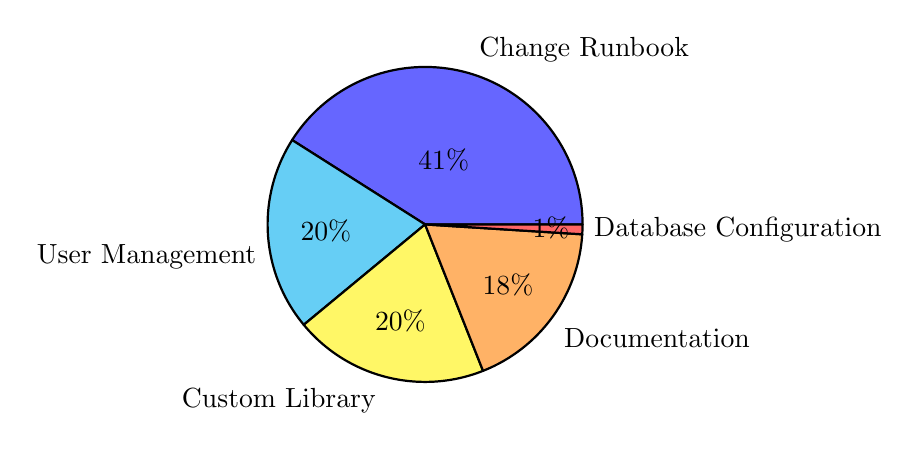
\begin{tikzpicture}
            \pie[radius=2]{41/Change Runbook,
                20/User Management,
                20/Custom Library,
                18/Documentation,
                1/Database Configuration
                }
        \end{tikzpicture}
    \end{center}
    \caption[แผนภูมิรูปวงกลมแสดงสัดส่วนของ Story Points]{แผนภูมิรูปวงกลมแสดงสัดส่วนของ Story Points}
    \label{fig:story-point-pie-chart}
\end{figure}

\section{ช่วงระยะเวลาการทำงาน}ข้าพเจ้าได้เริ่มต้นทำงานที่ฟีเจอร์ xPlatform เป็นระยะเวลาประมาณ 3 เดือน โดยในช่วงเวลาดังกล่าว ข้าพเจ้าได้ทำงานร่วมกับทีม Fast Easy เป็นระยะเวลา 1 สัปดาห์หลังจากเสร็จสิ้นโปรเจกต์แรก และในระยะเวลาที่เหลือข้าพเจ้าได้มีส่วนร่วมในการทำงานในโปรเจกต์ขนาดกลางกับทีม xPlatform ซึ่งจะได้แผนปฏิบัติงานสหกิจศึกษาดังนี้

\newcommand{\gantttitlevertical}[1]{\gantttitle{\rotatebox{90}{#1}}{1}}
\newcommand{\gantttitles}[2]{%
  \foreach \x in {#1} {%
    \gantttitle{\x}{#2}%
  }%
}
\newcommand{\blackcell}{
    \ganttbar[bar/.append style={fill opacity=1, pattern=crosshatch, pattern color=black},progress=100,inline=false]{}{16}{16}}

% link: https://tex.stackexchange.com/a/579761
\begin{table}[H]
    \centering
    \begin{ganttchart}[
        y unit title=0.5cm,
        y unit chart=0.6cm,
        x unit =0.6cm,
        % vgrid={draw=lightgray,line width=0.2pt},
        % hgrid={draw=lightgray,line width=0.2pt},
        vgrid,
        hgrid,
        title height=1,
        title/.style={fill=none, draw=black, line width=0.2pt},
        title label font=\footnotesize,
        bar/.style={fill=gray, fill opacity=0.5},
        bar height=1,
        bar top shift=0,
        progress label text={},
        group right shift=0,
        group height=.6,
        group peaks width={0.2},
        inline, 
        bar label node/.style={text width=2.75cm,
                               align=right,
                               anchor=east,
                               font=\small}
       ]{1}{16}
   
    \gantttitle{2024}{16}\\
                 
    \gantttitle{ก.ค.}{4} \gantttitle{ส.ค.}{4} \gantttitle{ก.ย.}{4} \gantttitle{ต.ค.}{4}\\

    \gantttitles{1,2,3,4,1,2,3,4,1,2,3,4,1,2,3,4}{1}\\
    
    \ganttbar[progress=100,inline=false]
        {Change Runbook}{1}{9}
    \ganttbar[progress=100,inline=false]
        {}{11}{11}
        \\
    \ganttbar[progress=100,inline=false]
        {DB Configuration}{10}{10}
        \\
    \ganttbar[progress=100,inline=false]
        {Documentation}{12}{12}
    \ganttbar[progress=100,inline=false]
        {}{13}{13}
        \\ 
    \ganttbar[progress=100,inline=false]
        {Custom Library}{12}{14} 
        \\
    \ganttbar[progress=100,inline=false]
        {User Management}{12}{12}
    \ganttbar[progress=100,inline=false]
        {}{14}{15} 
        \\
     \ganttbar[progress=100,inline=false]
        {Others}{10}{11} 
    \ganttbar[progress=100,inline=false]
        {}{13}{14} 

    \end{ganttchart}
    \caption{ตารางแผนปฏิบัติงานสหกิจศึกษา}
    \label{tab:work-timeline}
\end{table}

\bibliography{self-coop-report}

\ifproject
\normalspacing
\appendix
\newcommand{\includepdfwithfirstpagefit}[1]{
    \includegraphics[width=\textwidth, height=\textheight, keepaspectratio]{#1}
    \includepdf[pages=2-, fitpaper=true, nup=1x1, frame=false]{#1}
}

\newcommand{\includepdfwithonepage}[1]{
    \includegraphics[width=\textwidth, height=\textheight, keepaspectratio]{#1}
}

\chapter{เอกสารเกี่ยวข้อง}

TODO add 3-4

\section{วศ.สก.-06}
\includepdfwithfirstpagefit{resources/bureaucrats/coop6.pdf}

\section{วศ.สก.-10}
\includepdfwithfirstpagefit{resources/bureaucrats/coop10.pdf}

\section{วศ.สก.-11}
\includepdfwithonepage{resources/bureaucrats/coop11.pdf}

\section{หนังสือยินยอมให้เผยแพร่รายงานปฏิบัติงานสหกิจศึกษา}
\includepdfwithonepage{resources/bureaucrats/publish-consent.pdf}

\chapter{ตารางแสดงรายละเอียดการสะสม Story Points}
\section{ตารางแสดงรายละเอียดการสะสม Story Points ของ Change Runbook}
\begin{table}[H]
    \centering
    \begin{tabularx}{0.85\textwidth}{X|c}
        \attr{รายละเอียด} & \attr{Story Points} \\
        \hline\hline
        \textbf{Change Runbook} & \textbf{42} \\
        getActivity & 2 \\
        getActivityInfo & 1 \\
        searchActivity & 1 \\
        getRequiredActivity & 2 \\
        getUserActivityPermission &	1 \\
        getResponsibleUser & 1 \\
        getLatestActivityMark &	1 \\
        Initial database design & 1 \\
        Import Jira - getField & 3 \\
        Import Jira - getPreview & 1 \\
        Import Jira - activity & 5 \\
        Import CSV - getField & 1 \\
        Import CSV - getPreview & 1 \\
        Import CSV - activity & 2 \\
        Optimise getActivity with resolver facilitator & 2 \\
        Autogeneration on activity group and activity hashtag on create/update activity & 1 \\
        Autodeletion on activity group and activity hashtag on update/remove activity & 1 \\
        Improve on change runbook .xlsx export & 5 \\
        getLatestImplementationDateTimeTo & 1 \\
        Implement previewUpdateActivityAffect and previewRemoveActivityAffect & 5 \\
        Implement update and remove activity time shift & 2 \\
        Change update/remove activity validation & 2 \\
        \hline\hline
        \textbf{รวม} & 42
    \end{tabularx}
    \caption{ตารางแสดงรายละเอียดการสะสม Story Points ของ Change Runbook}
    \label{tab:story-point-table}
  \end{table}

  \section{ตารางแสดงรายละเอียดการสะสม Story Points อื่น ๆ}
  \begin{table}[H]
      \centering
      \begin{tabularx}{0.85\textwidth}{X|c}
          \attr{รายละเอียด} & \attr{Story Points} \\
          \hline\hline
          \textbf{User Management} & \textbf{1} \\
          TODO & 2351 \\
          TODO & 1954 \\
          \hline
          \textbf{Documentation} & \textbf{1} \\
          TODO & 2351 \\
          TODO & 1954 \\
          \hline
          \textbf{Custom Library} & \textbf{1} \\
          TODO & 2351 \\
          TODO & 1954 \\
          \hline
          \textbf{Others} & \textbf{1} \\
          TODO & 2351 \\
          TODO & 1954 \\
          \hline\hline
          \textbf{รวม} & TODO
      \end{tabularx}
      \caption{ตารางแสดงรายละเอียดการสะสม Story Points อื่น ๆ }
      \label{tab:story-point-table-others}
    \end{table}

\chapter{การใช้งานซอฟต์แวร์}

\section{การใช้งานฟีเจอร์ Change Runbook}
\subsection{การสร้าง Activity}
\begin{center}
    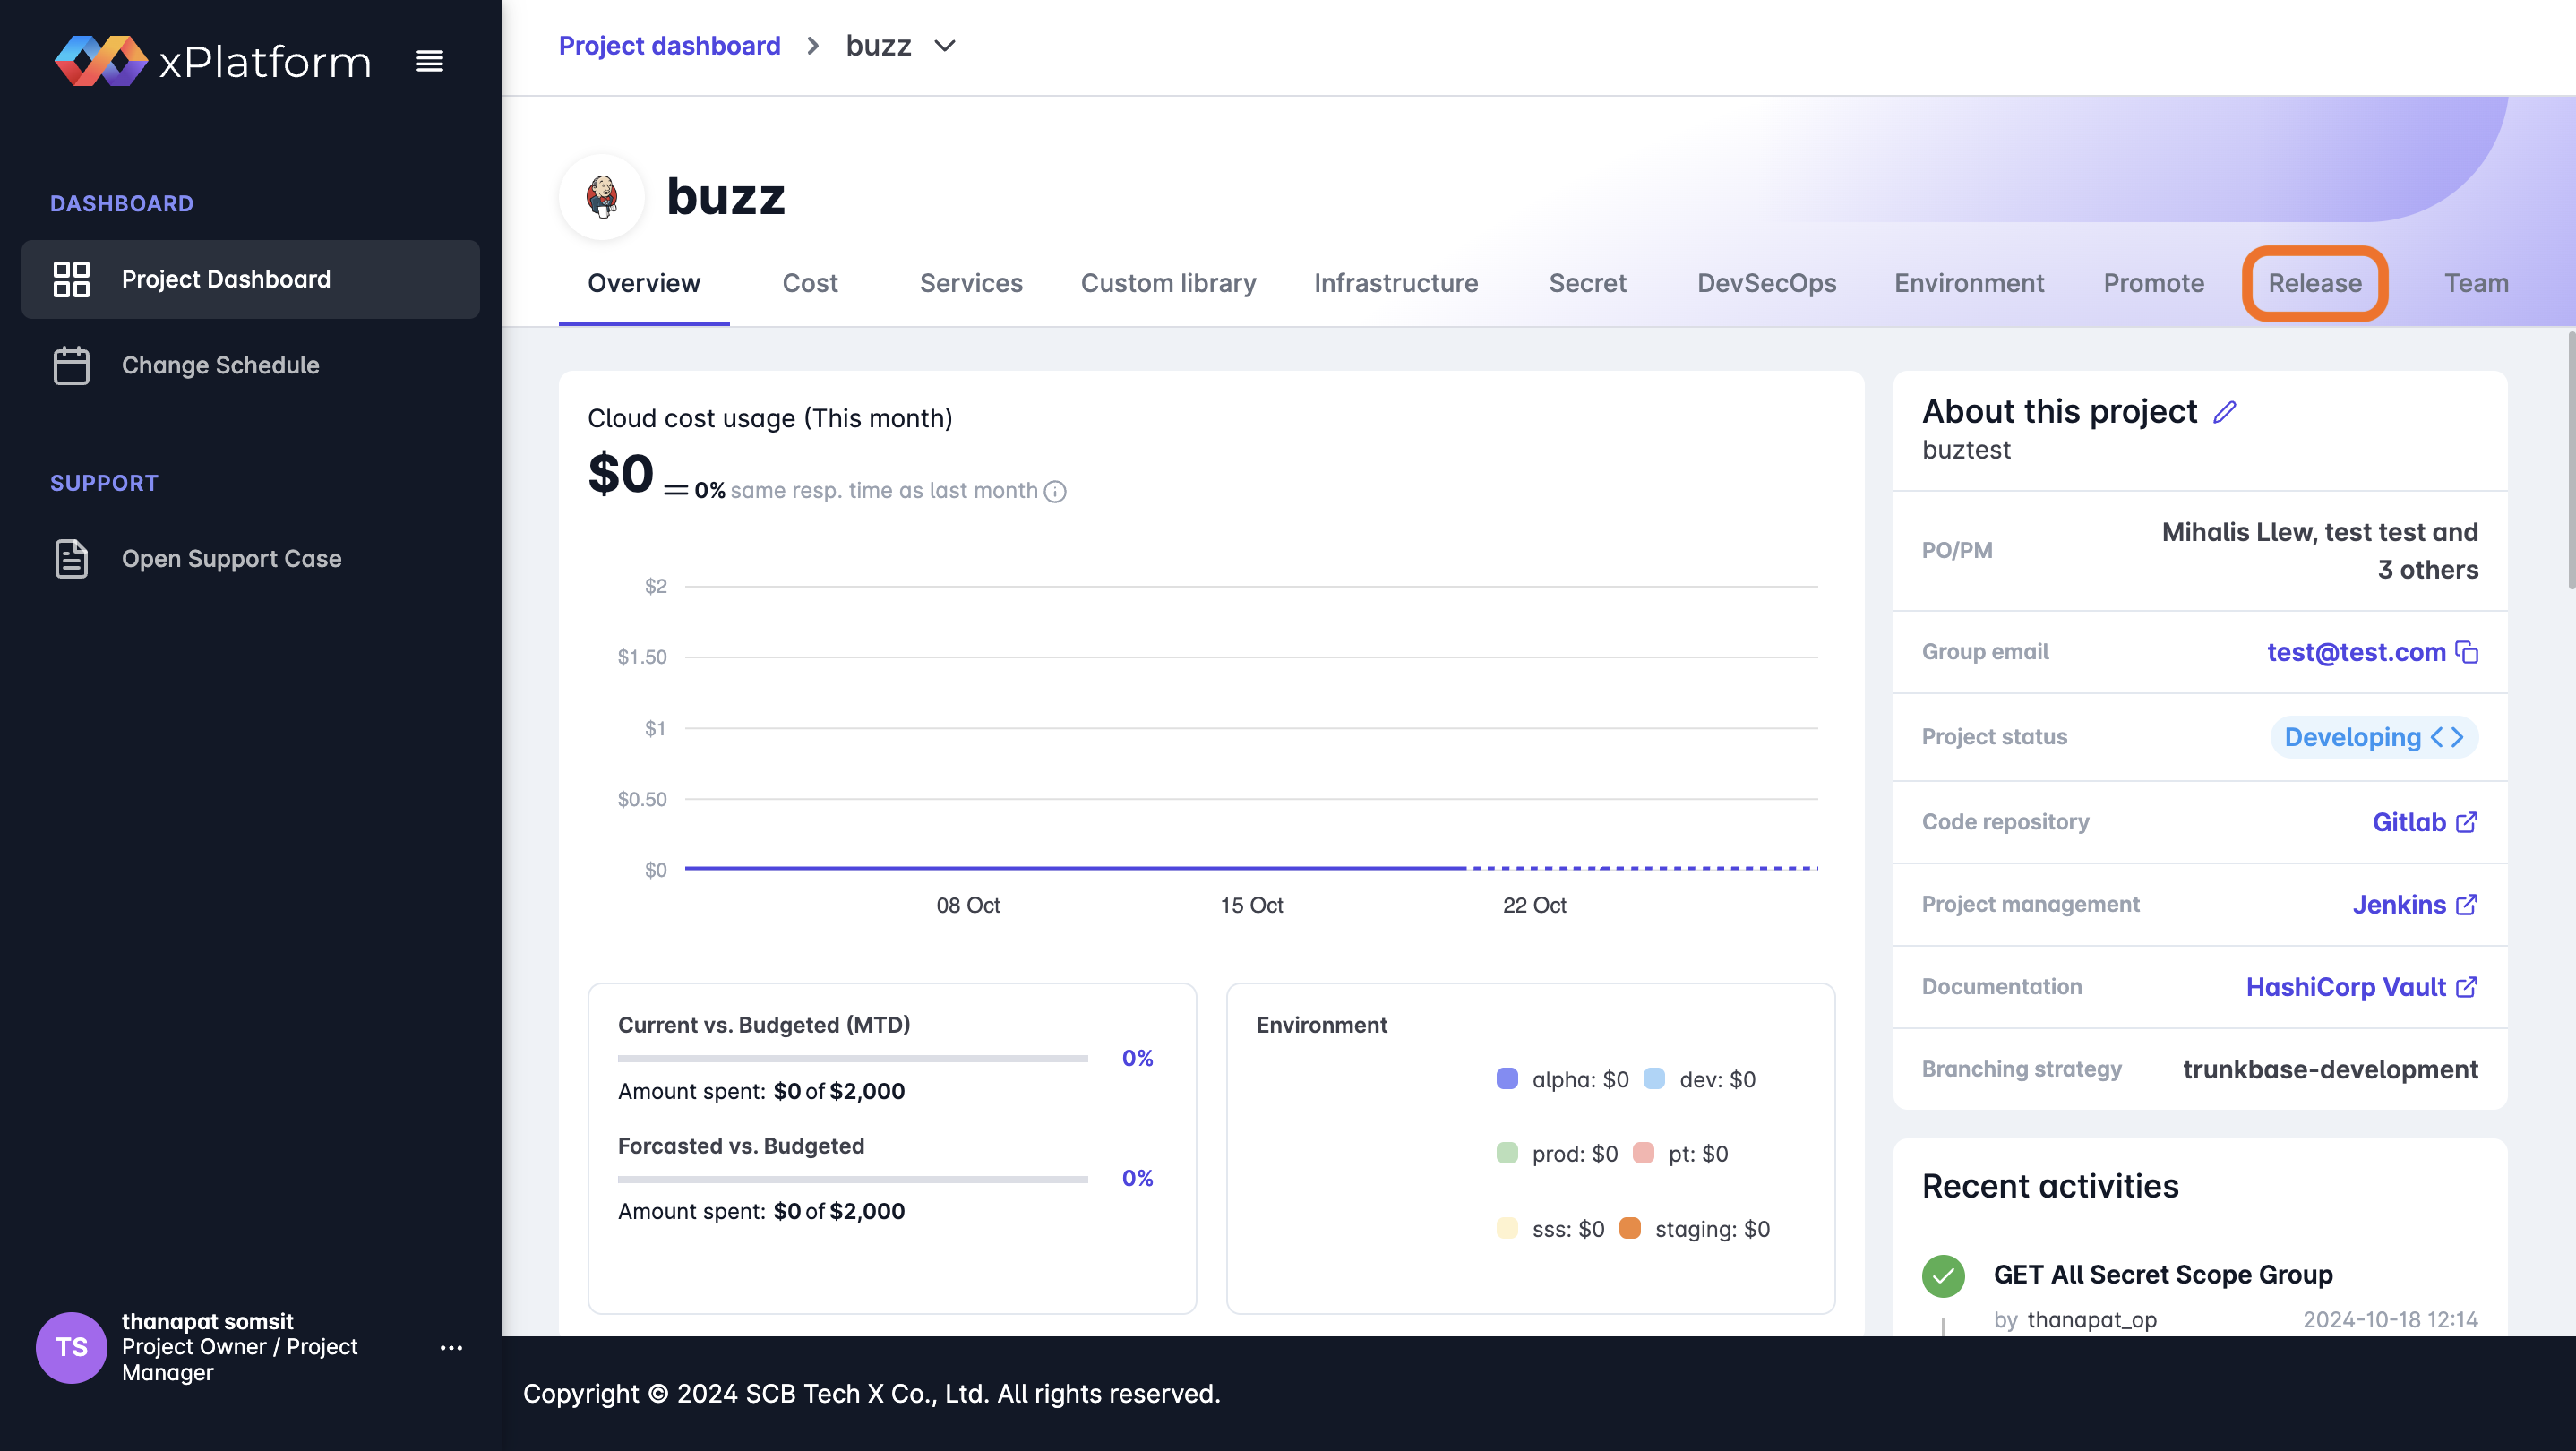
\includegraphics[width=\linewidth]{resources/pages/change-runbook/create-activity/1.png}

    \vspace{1in}

    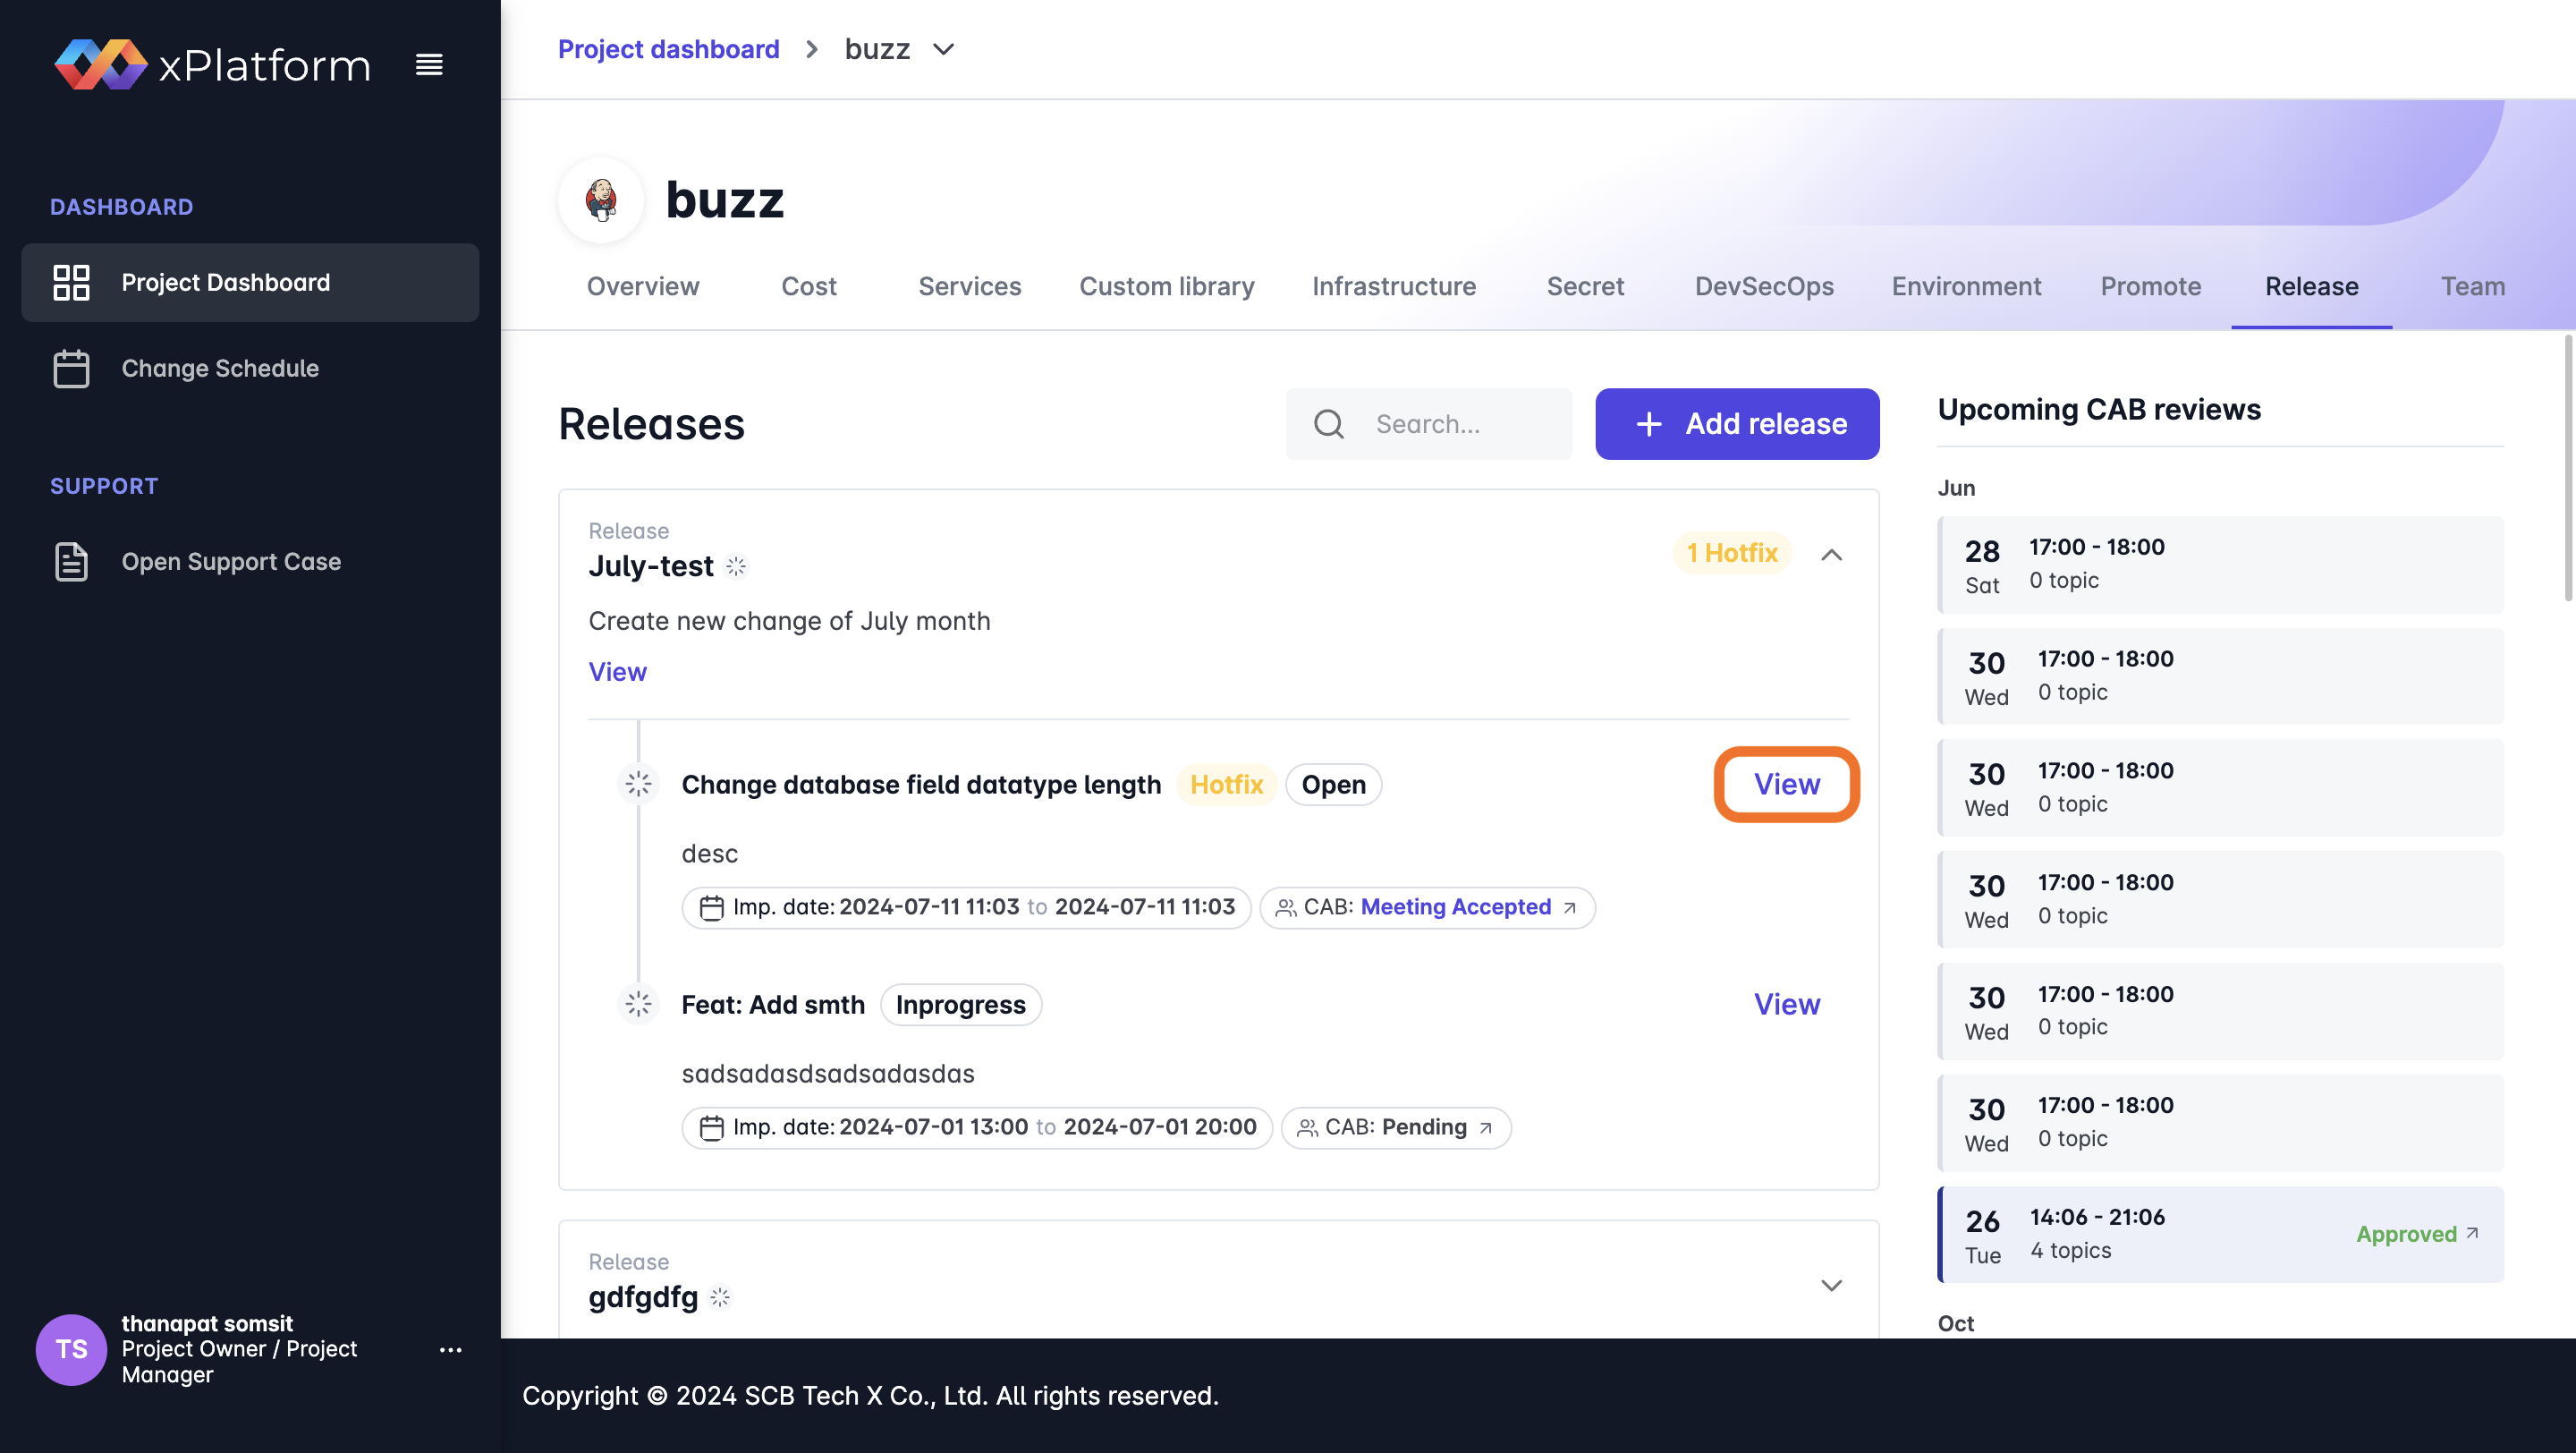
\includegraphics[width=\linewidth]{resources/pages/change-runbook/create-activity/2.png}
\end{center}
\begin{center}
    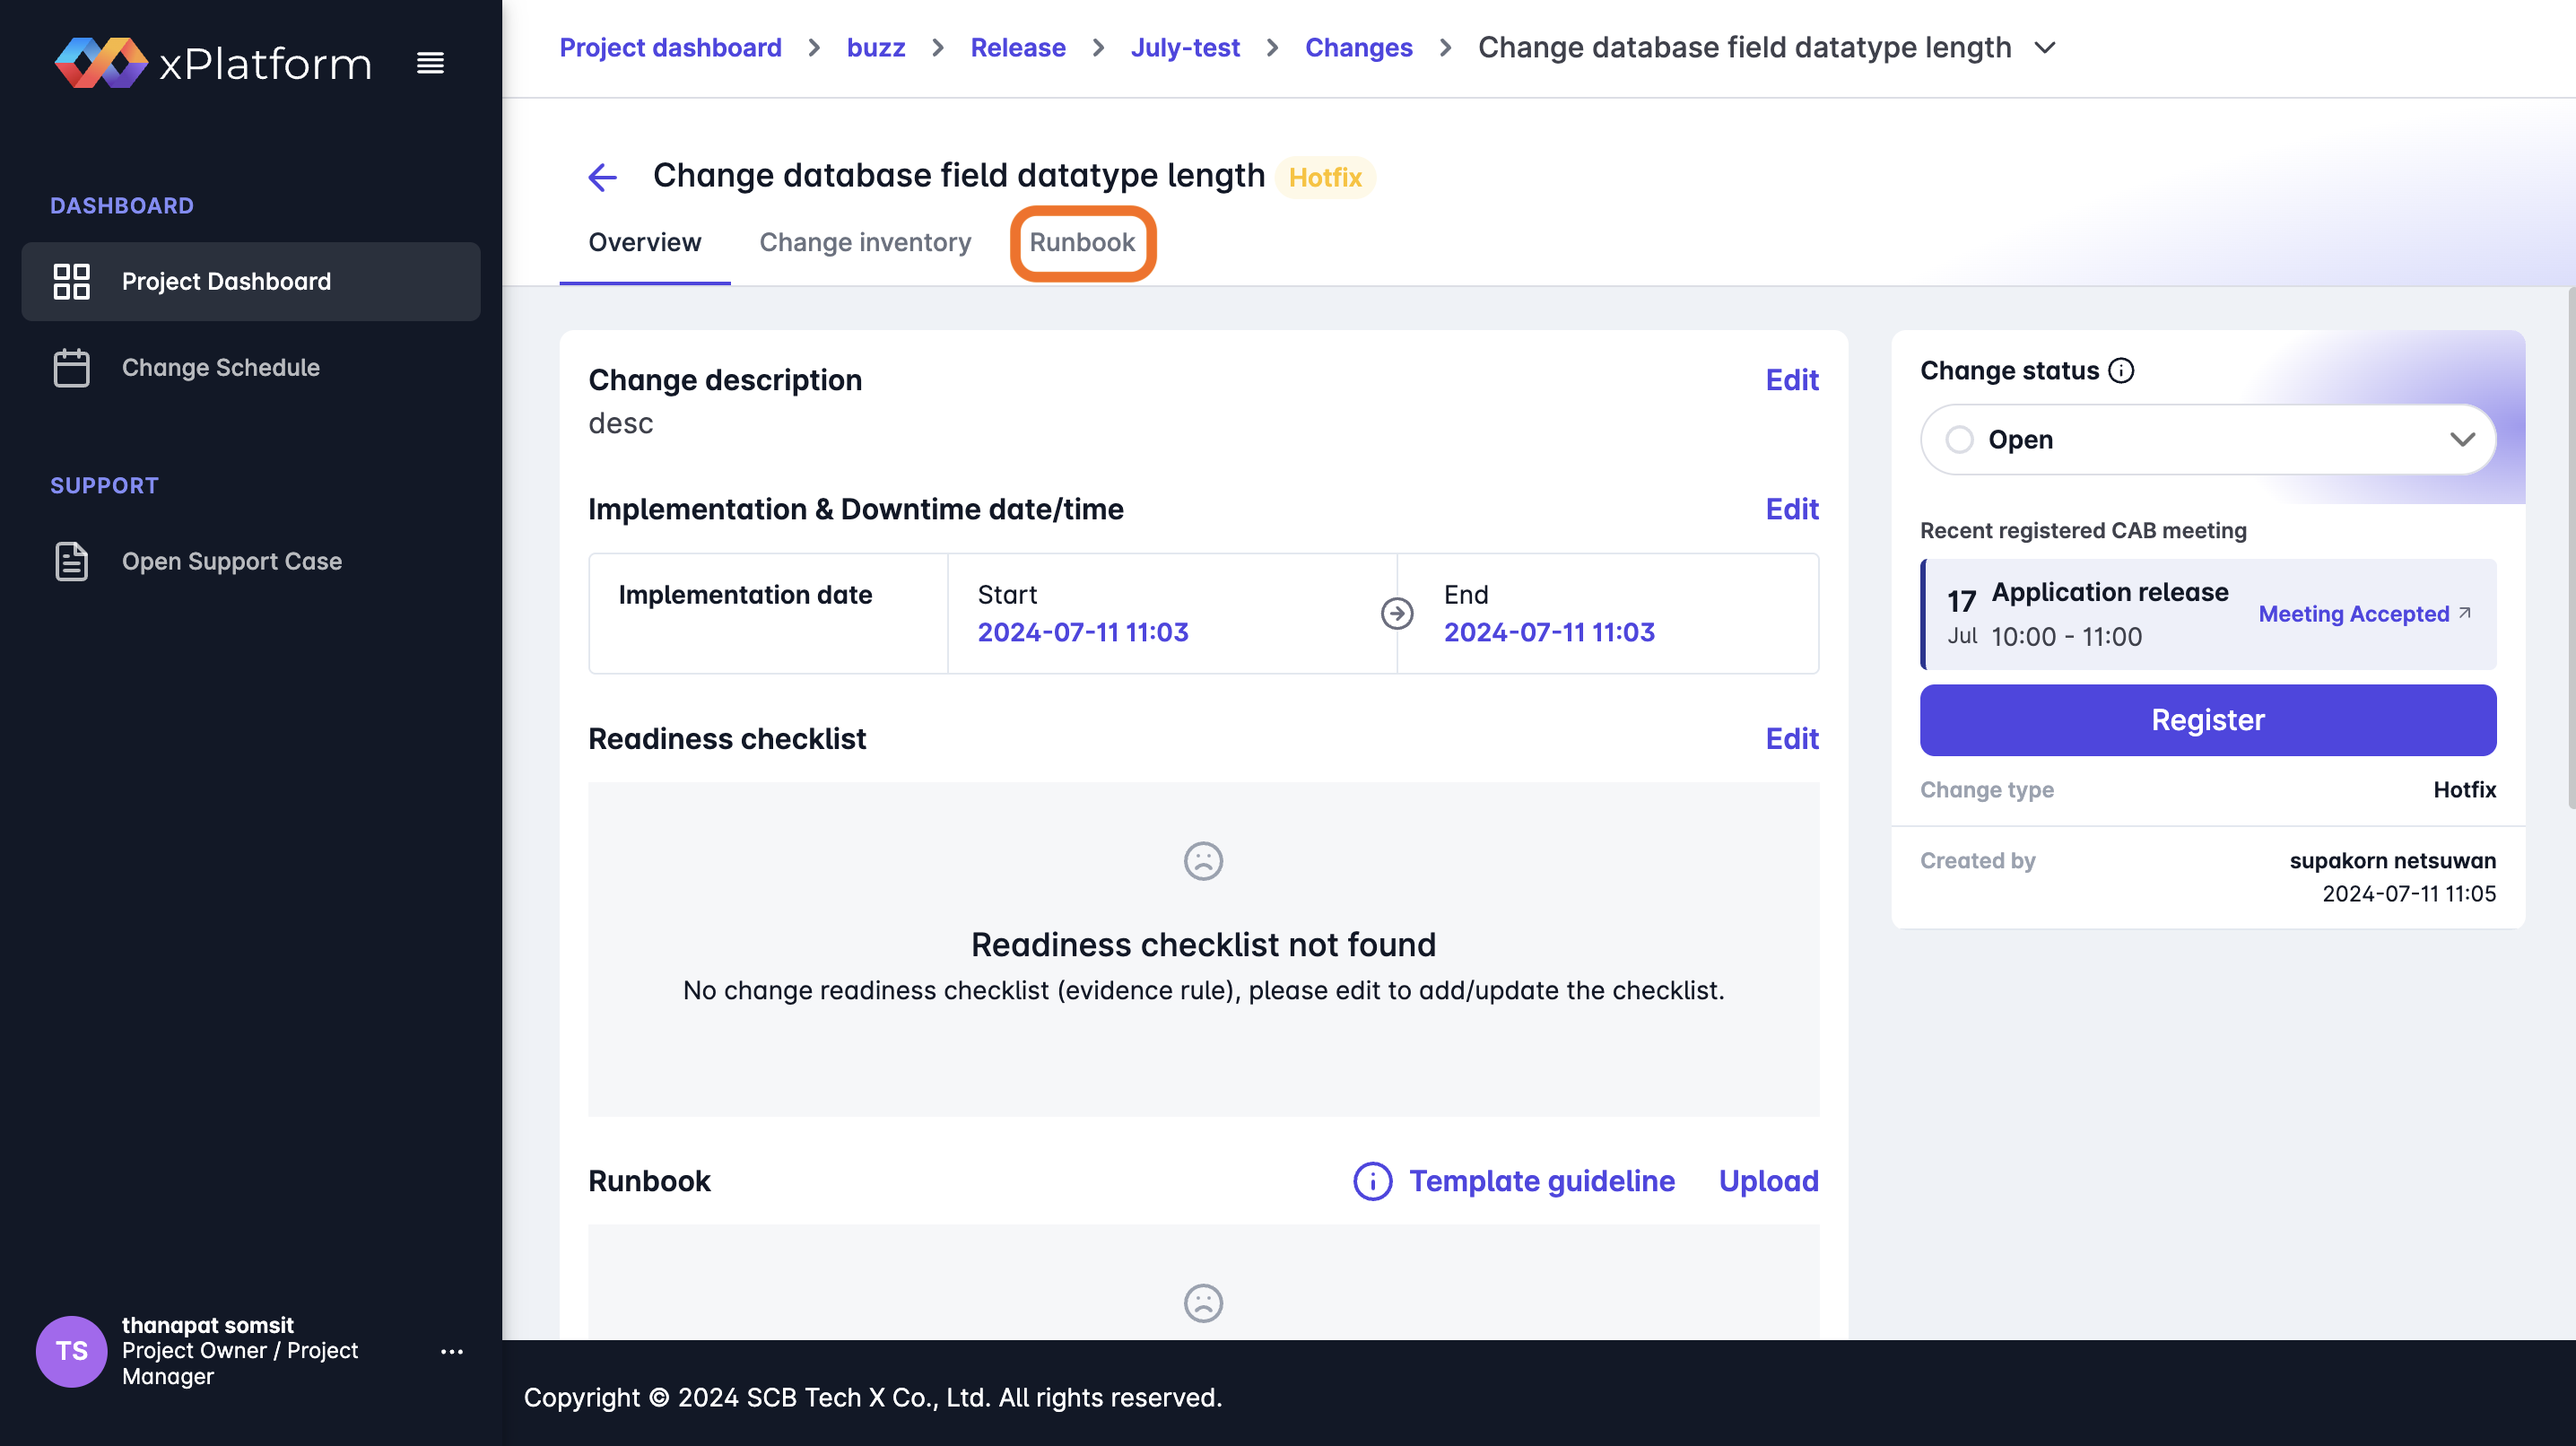
\includegraphics[width=\linewidth]{resources/pages/change-runbook/create-activity/3.png}

    \vspace{1in}

    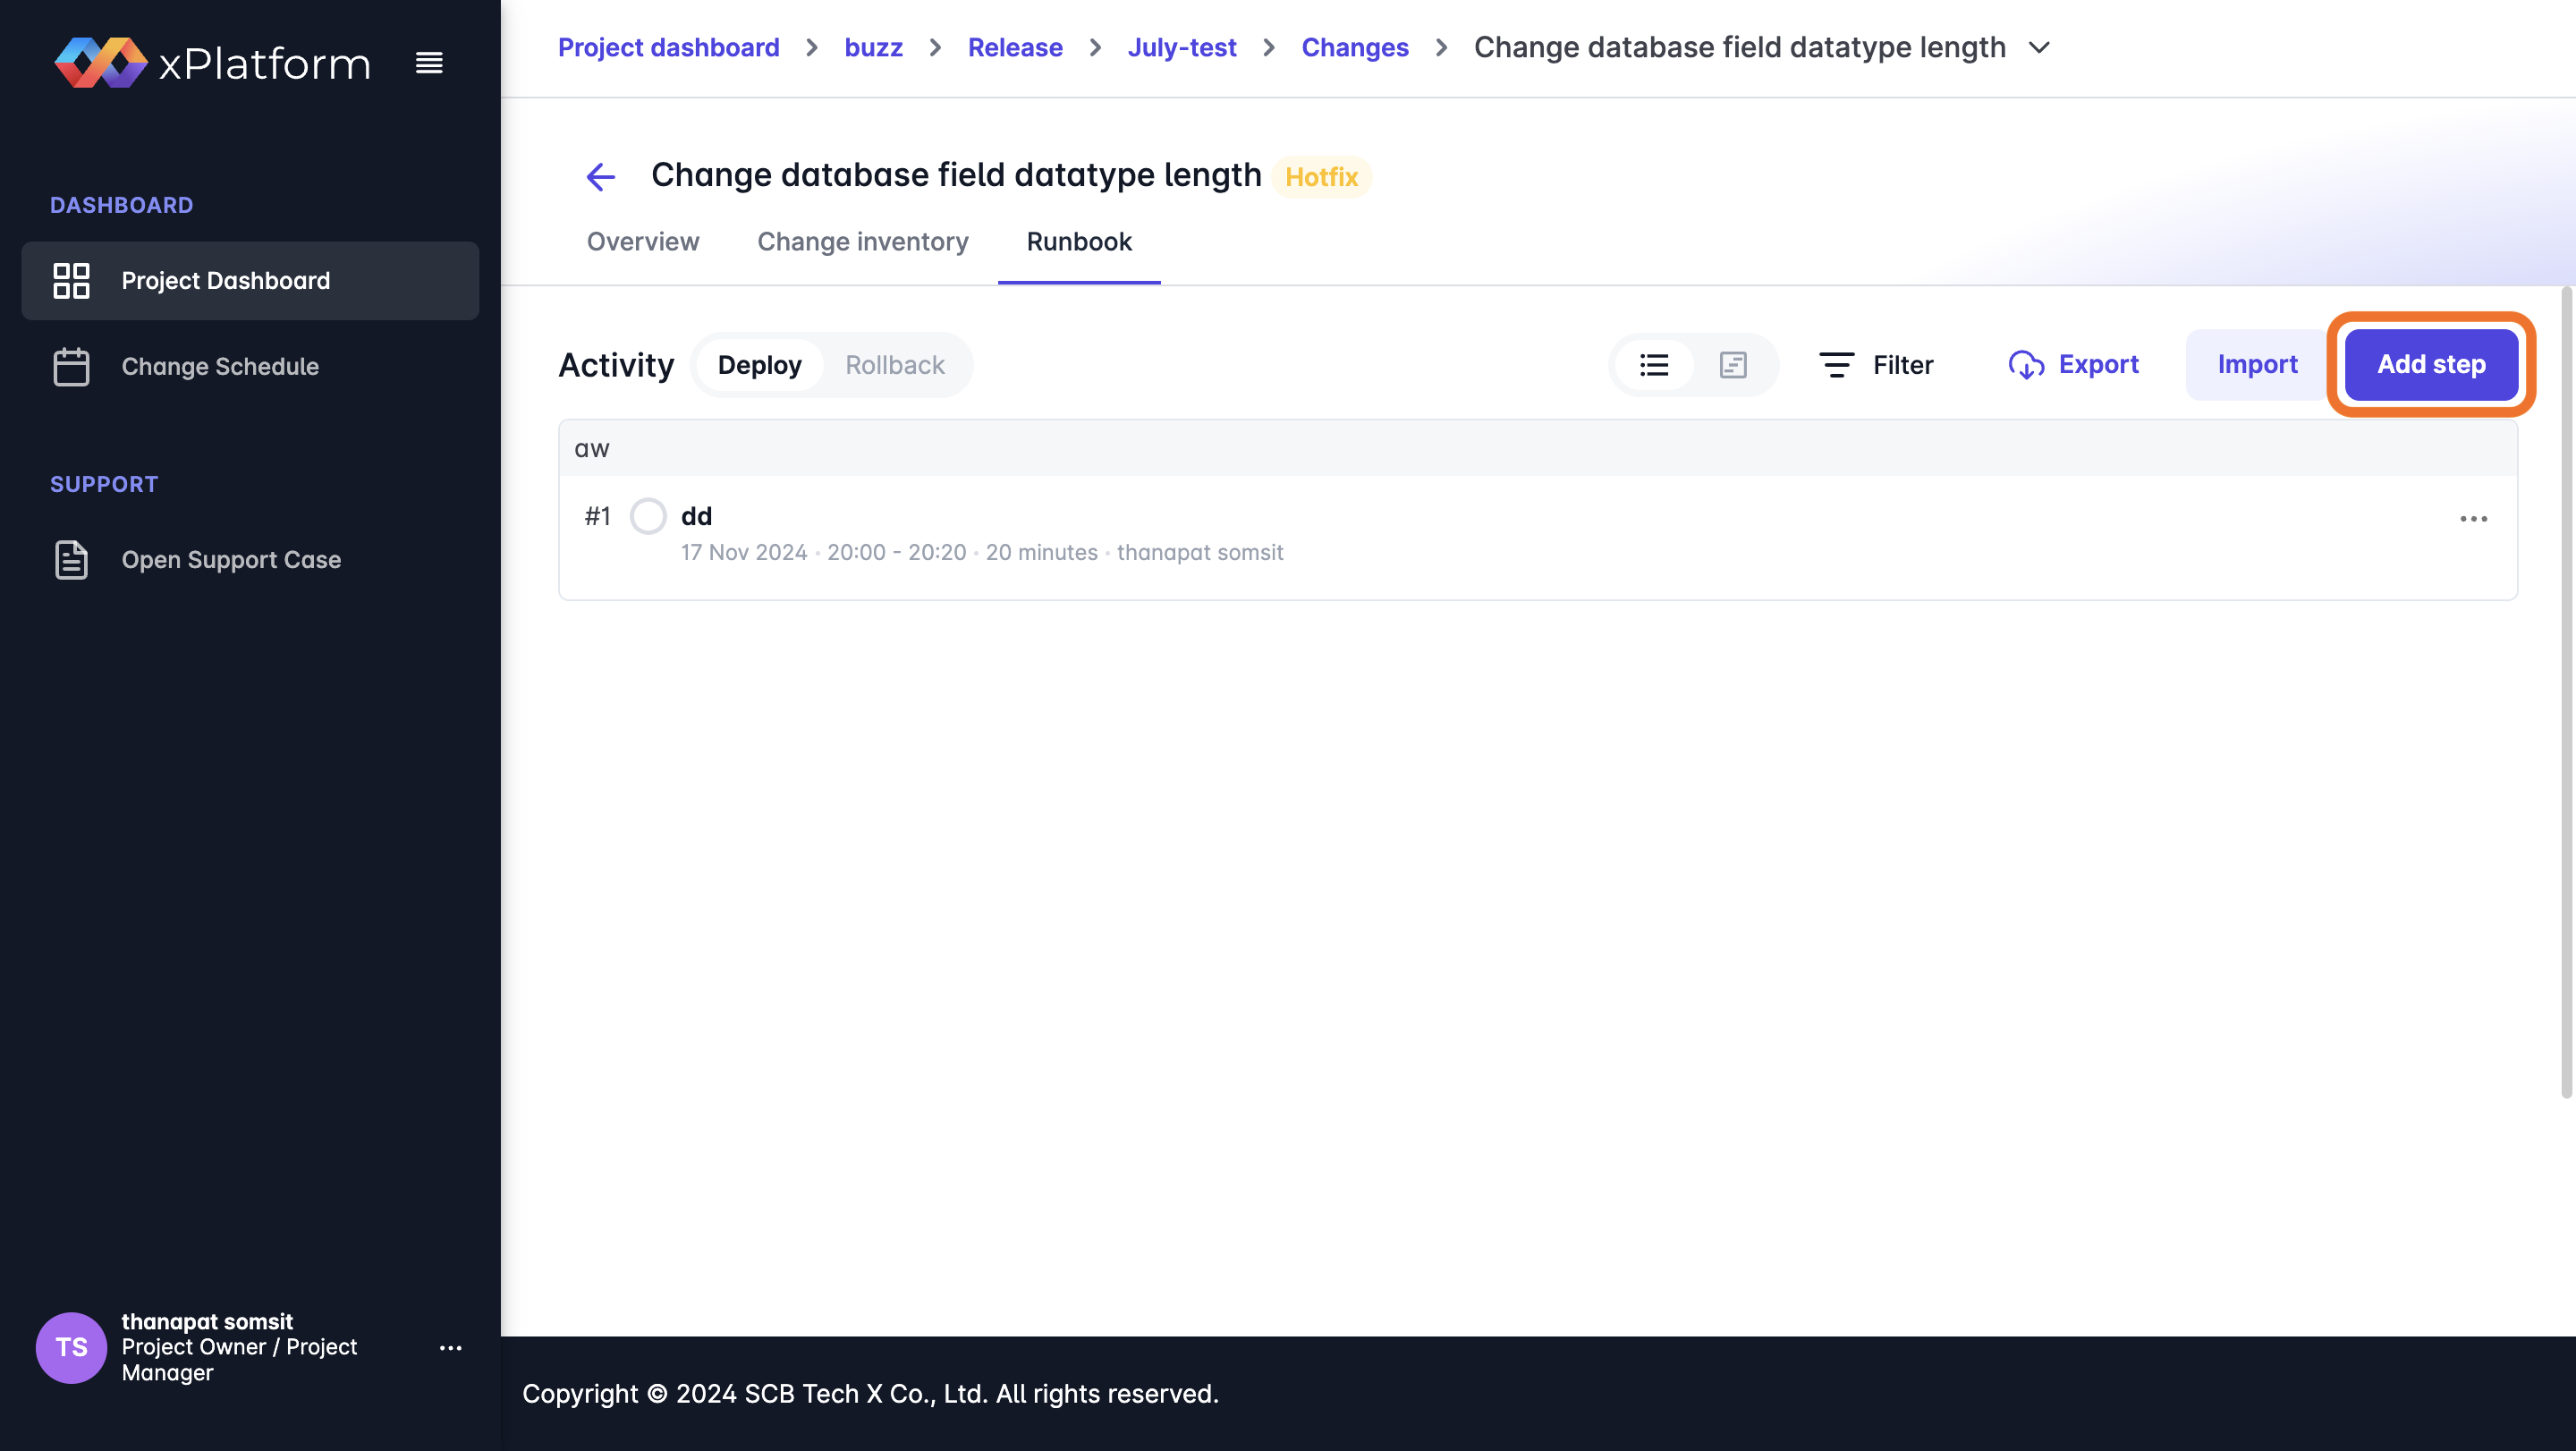
\includegraphics[width=\linewidth]{resources/pages/change-runbook/create-activity/4.png}
\end{center}

\begin{figure}[H]
    \begin{center}
        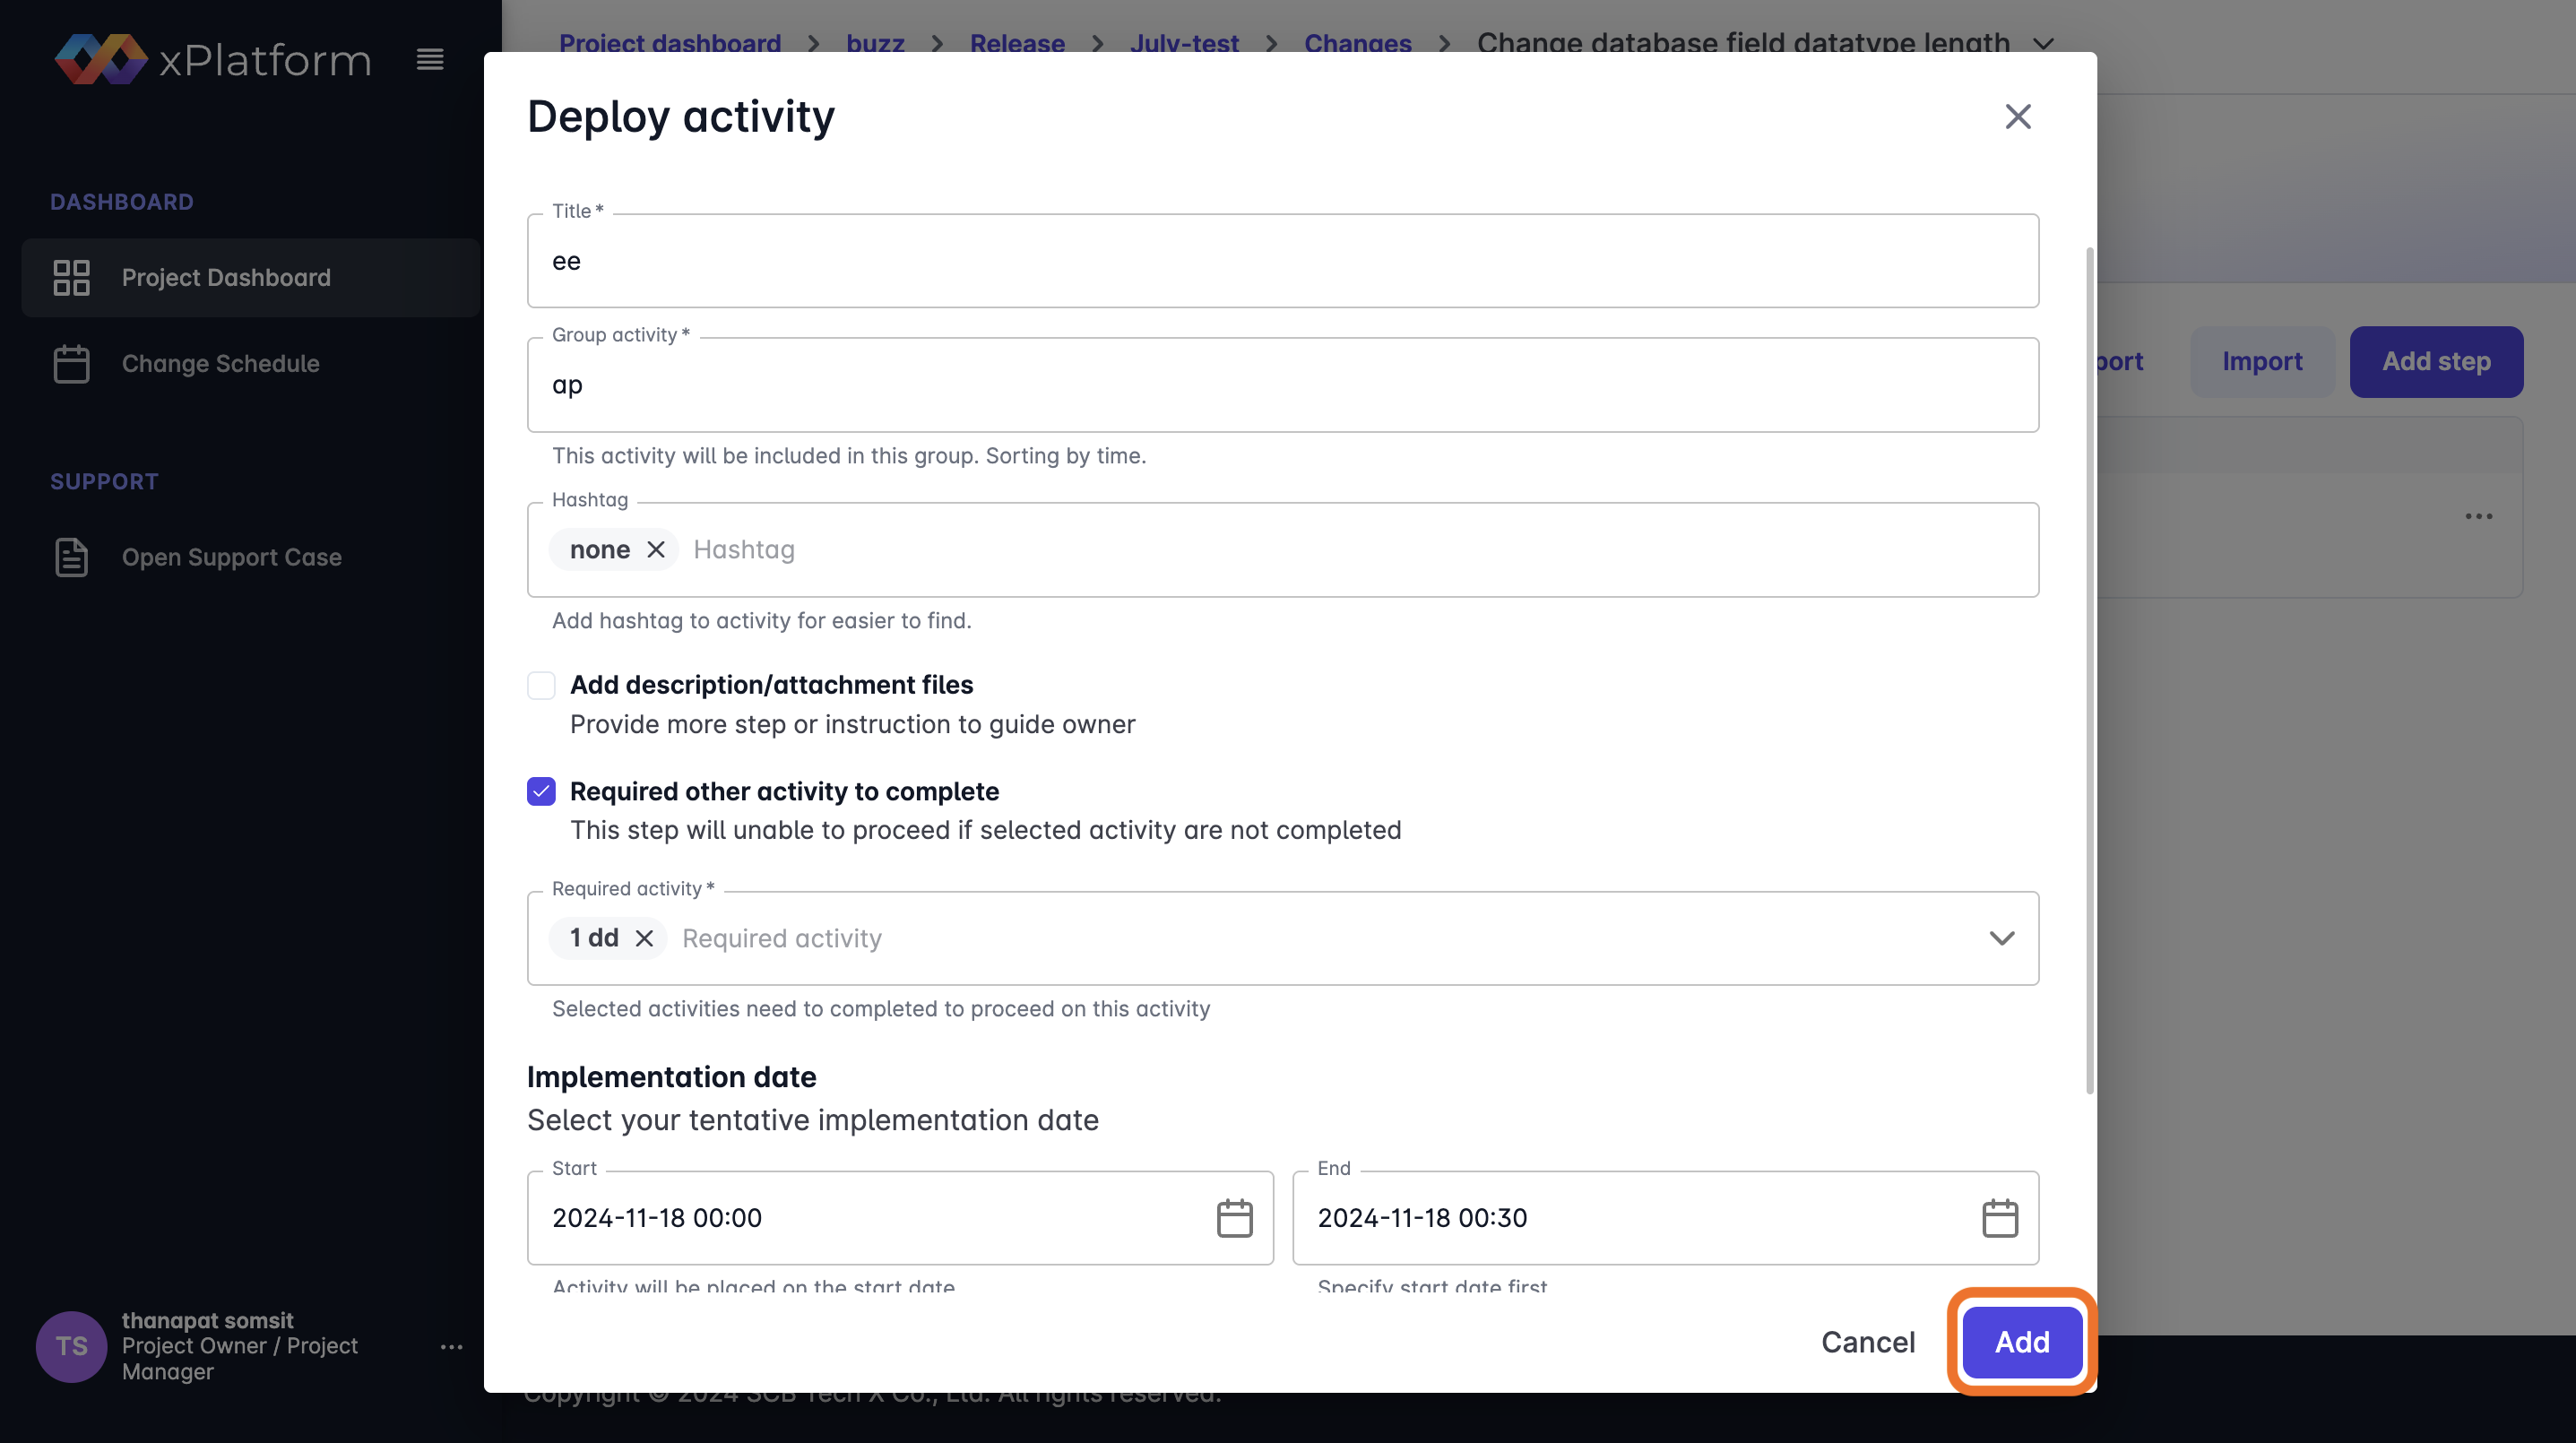
\includegraphics[width=\linewidth]{resources/pages/change-runbook/create-activity/5.png}
    
        \vspace{1in}
    
        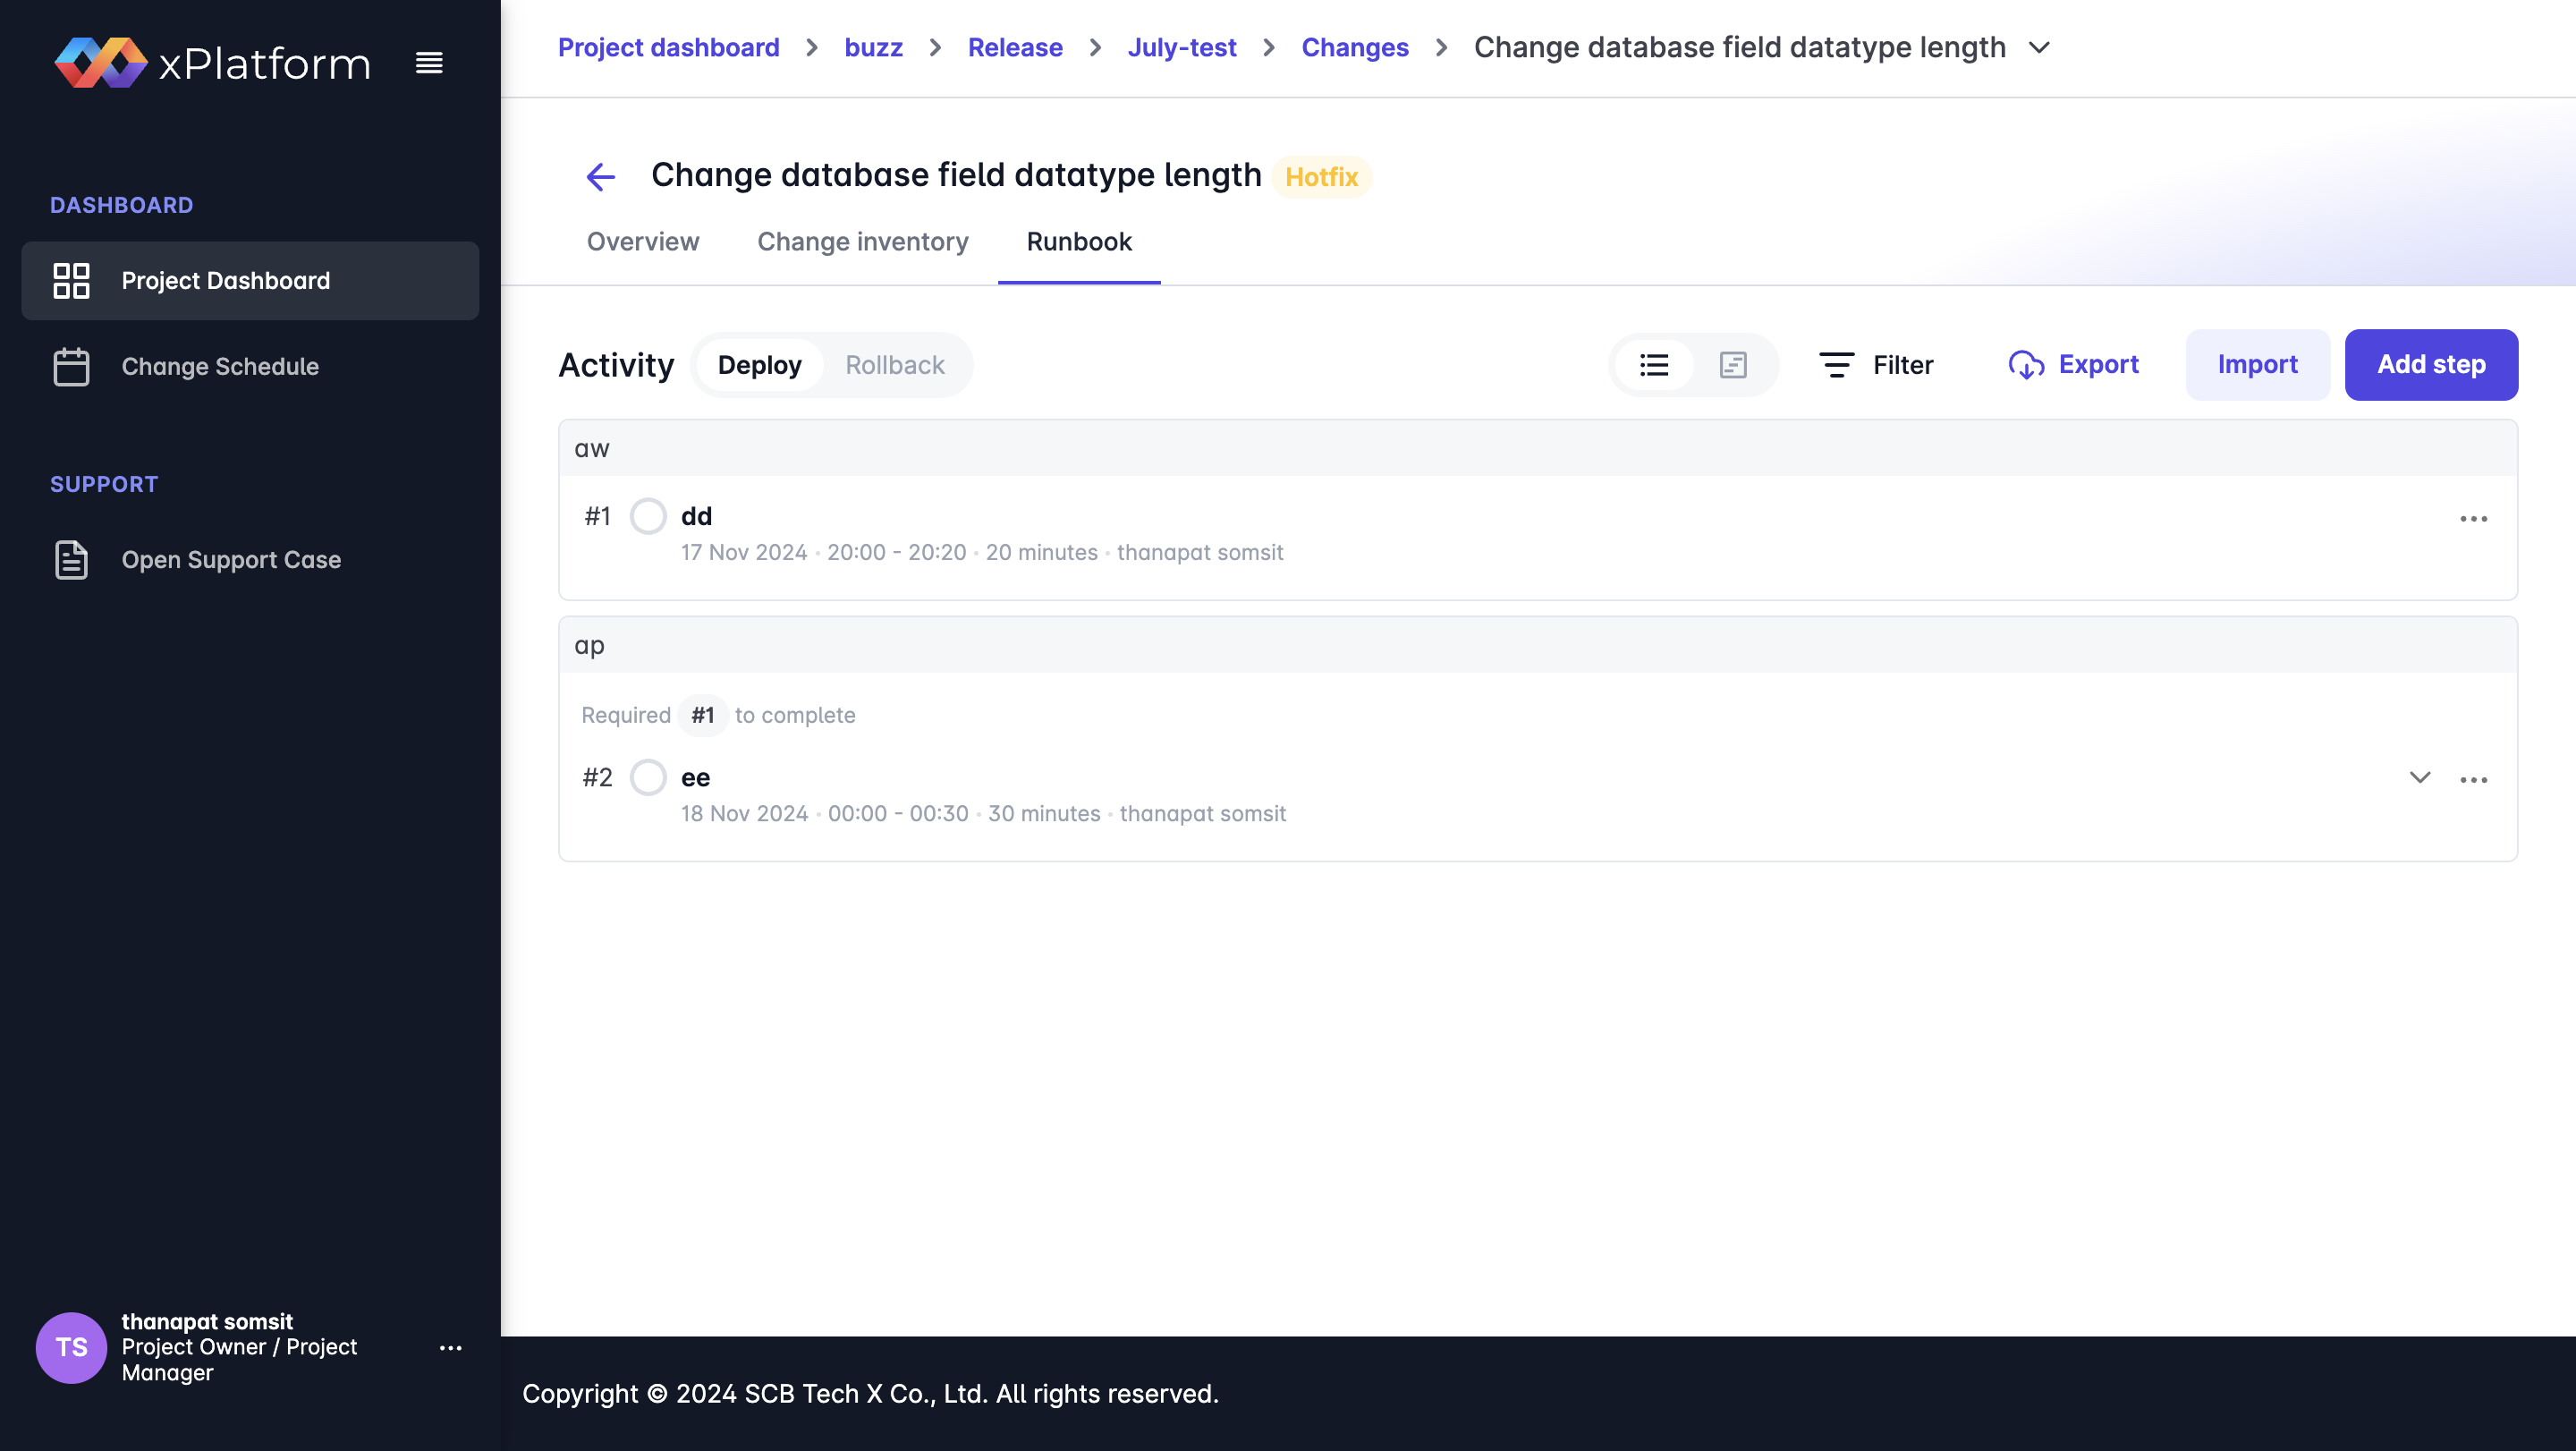
\includegraphics[width=\linewidth]{resources/pages/change-runbook/create-activity/6.png}
    \end{center}
    \caption[การสร้าง Activity]{การสร้าง Activity}
  \label{fig:create-activity}
\end{figure}

\newpage
\subsection{การเปลี่ยนแปลง Activity}
\begin{center}
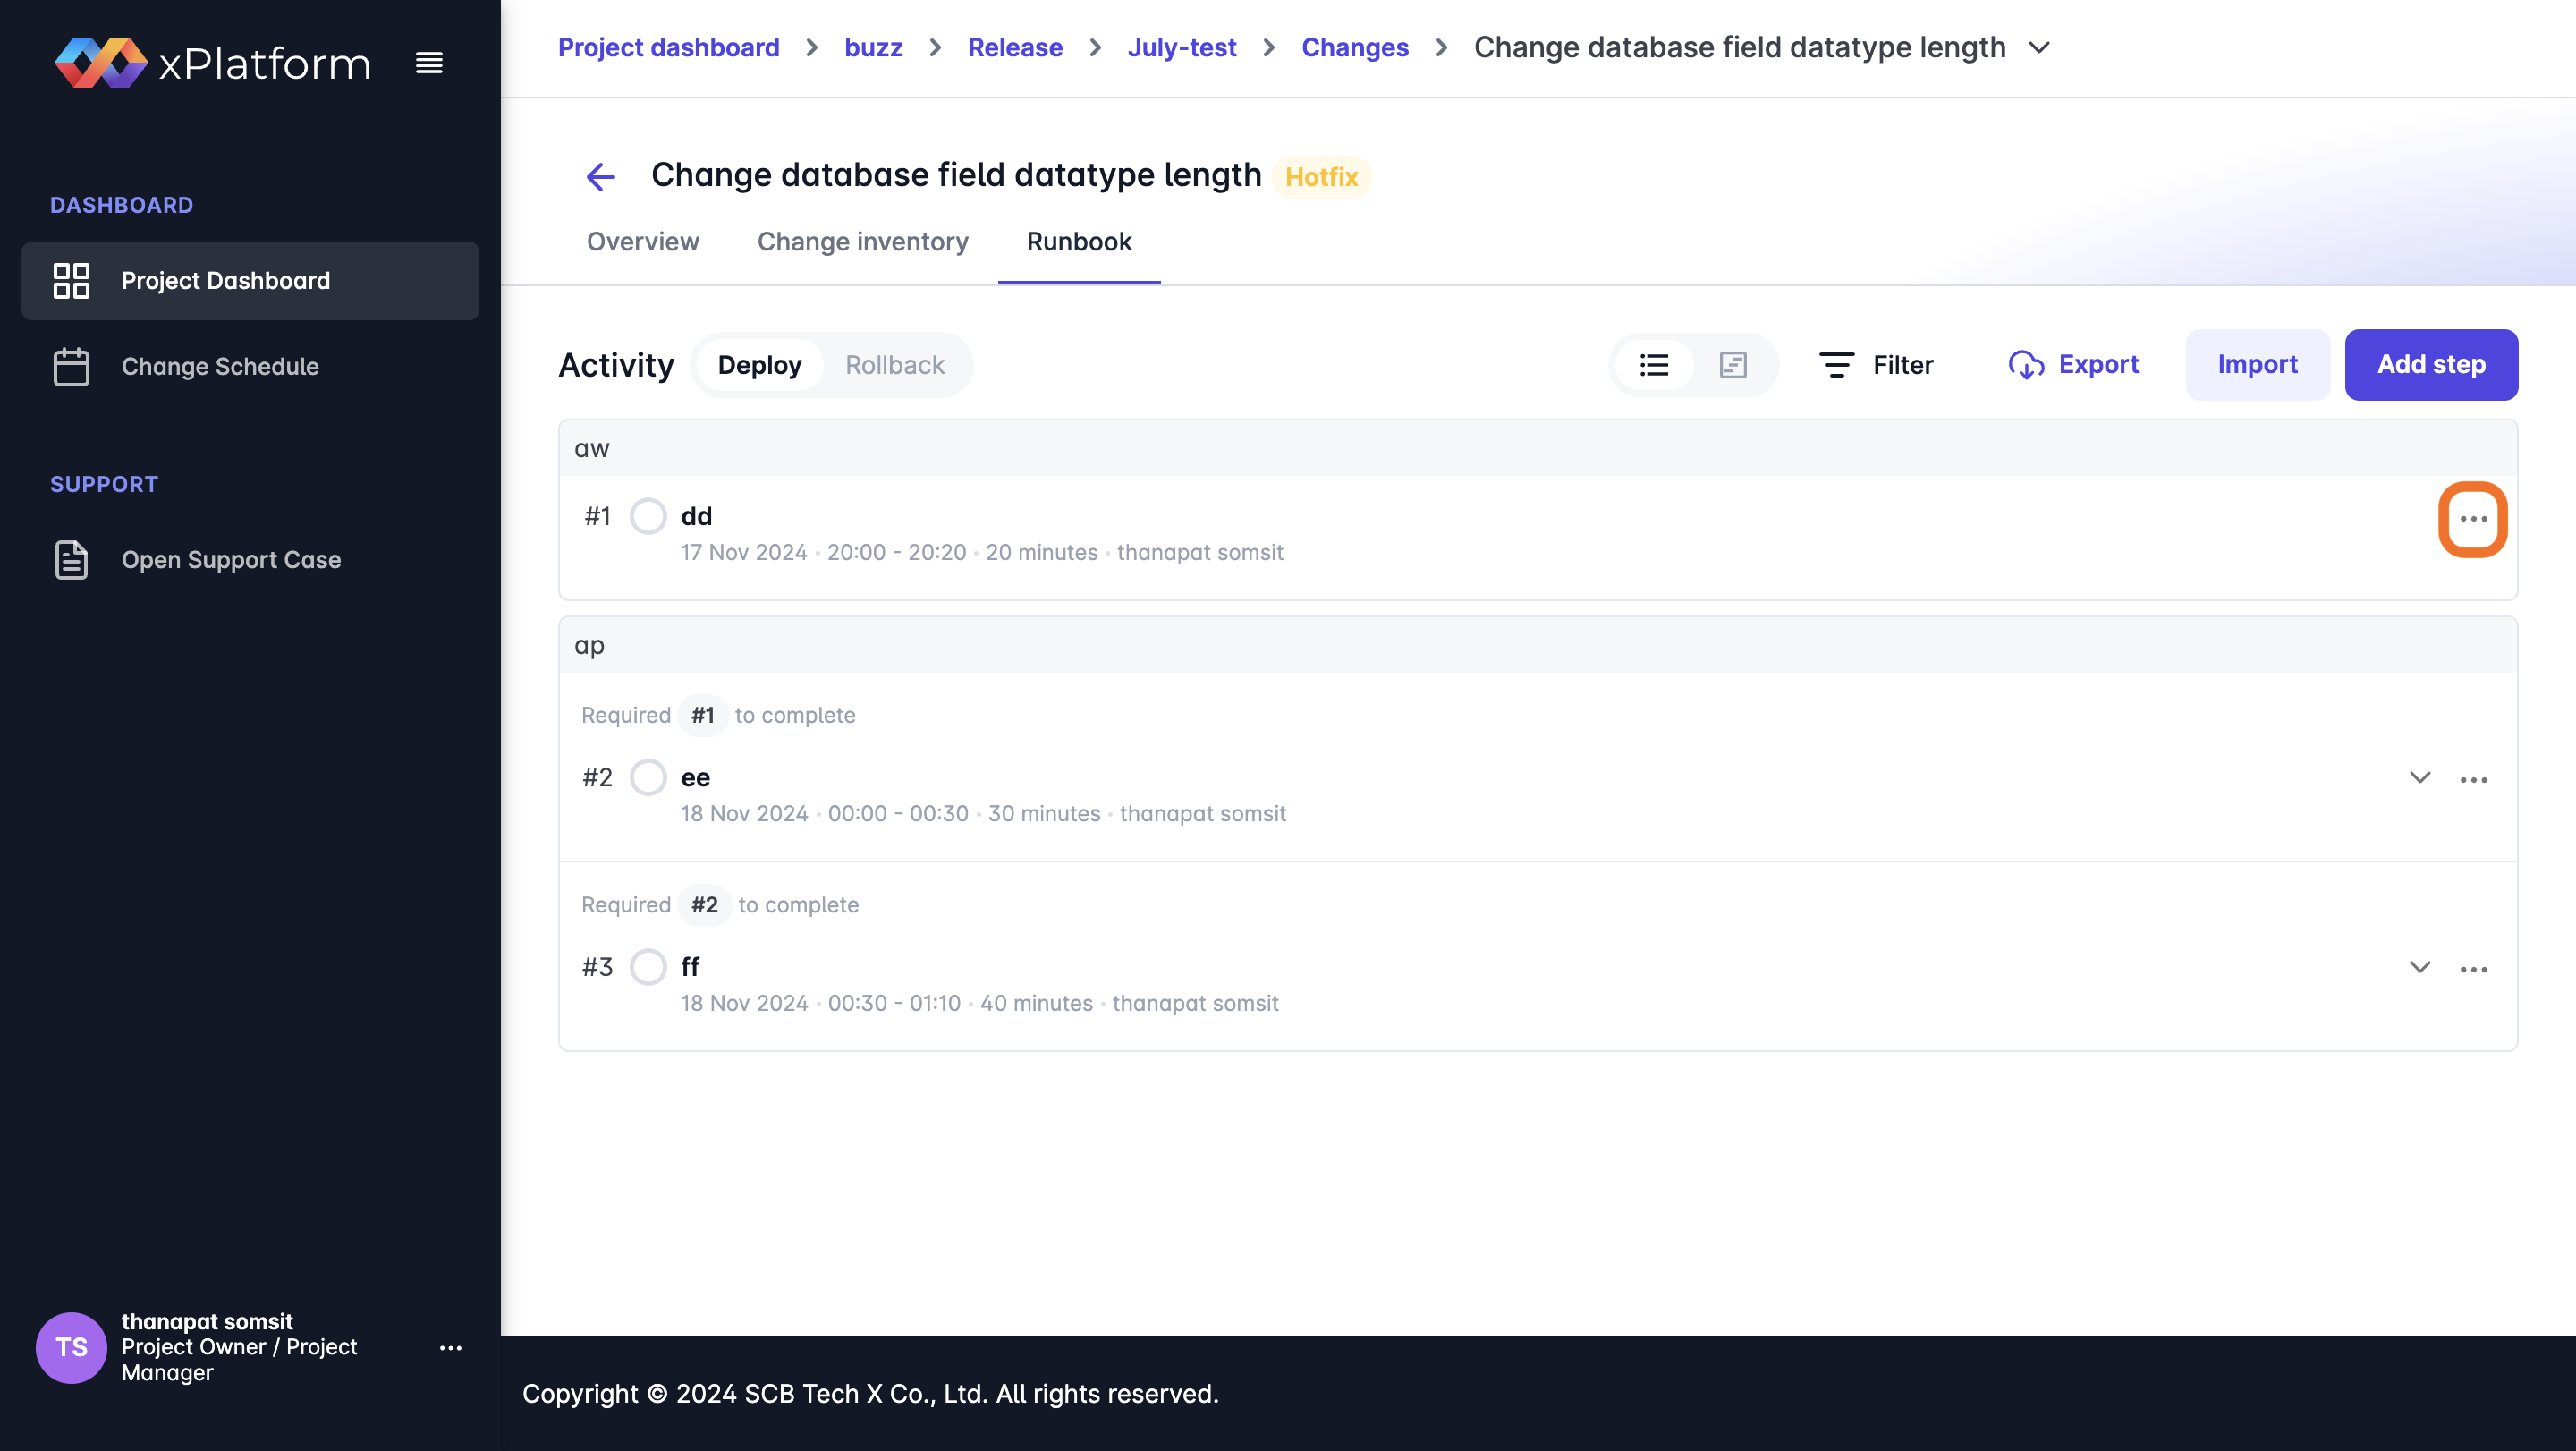
\includegraphics[width=\linewidth]{resources/pages/change-runbook/update-activity/7.png}

\vspace{1in}

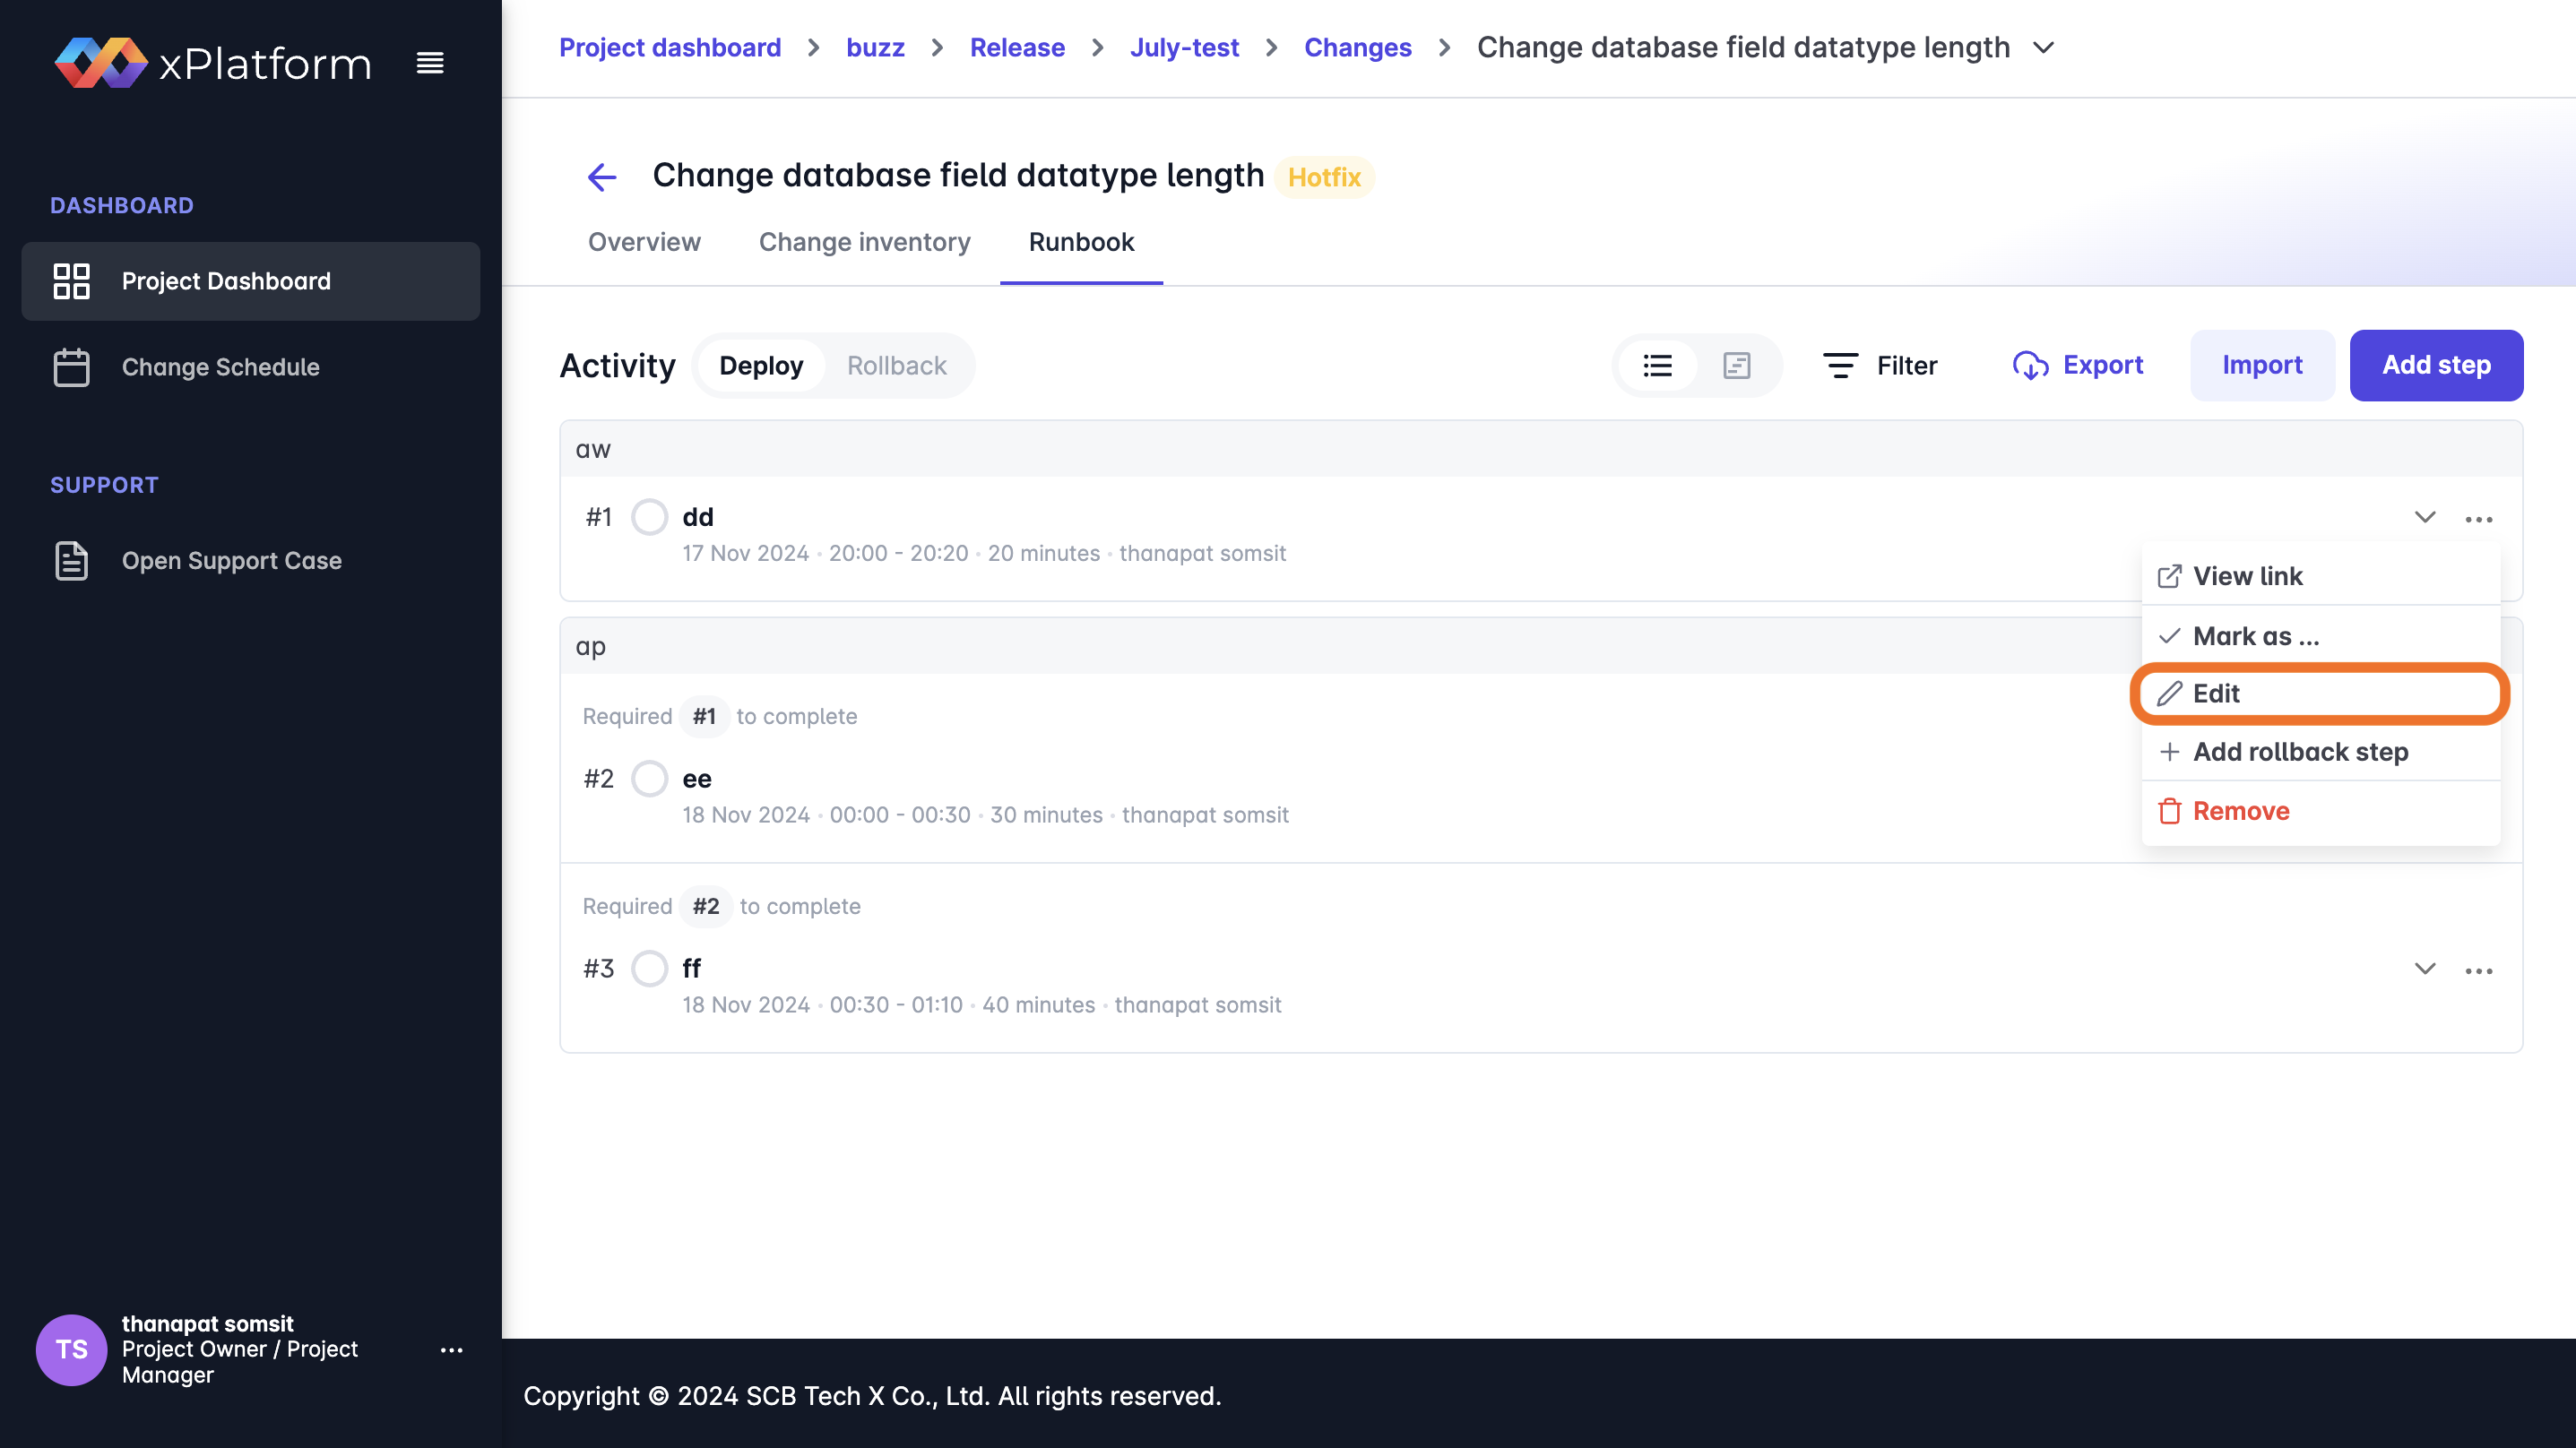
\includegraphics[width=\linewidth]{resources/pages/change-runbook/update-activity/8.png}
\end{center}

\begin{figure}[H]
\begin{center}
    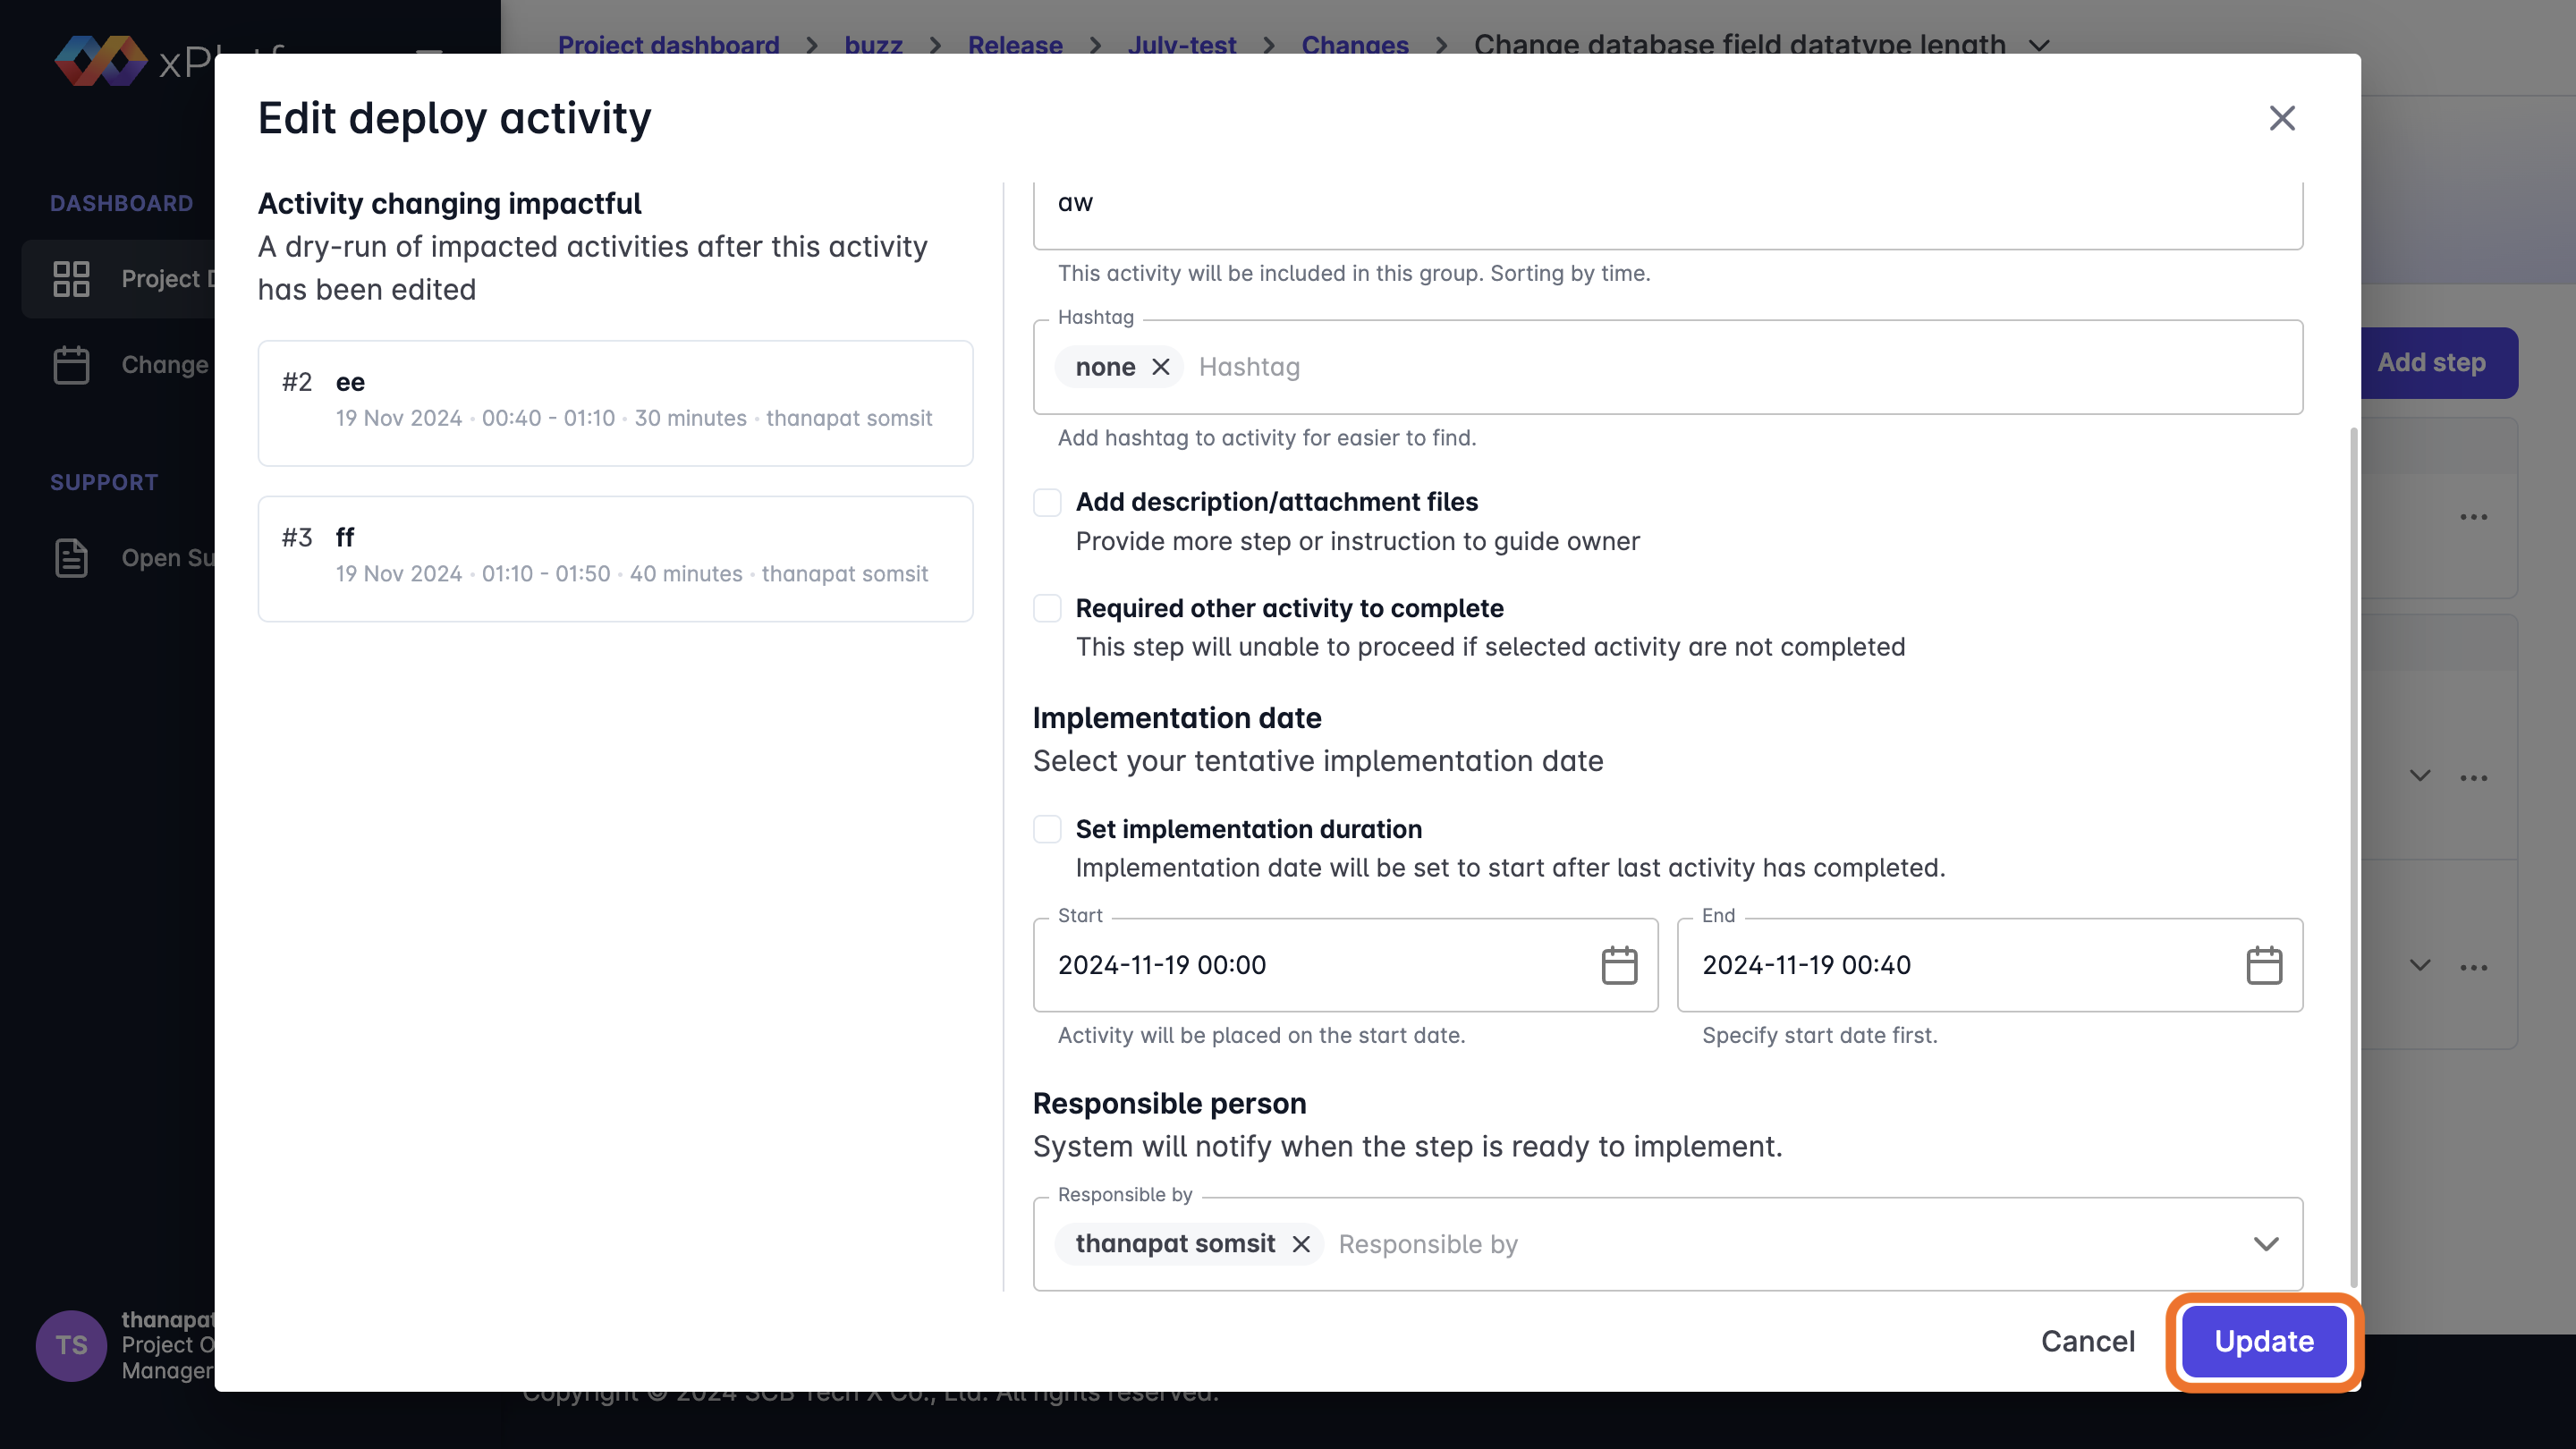
\includegraphics[width=\linewidth]{resources/pages/change-runbook/update-activity/9.png}

    \vspace{1in}

    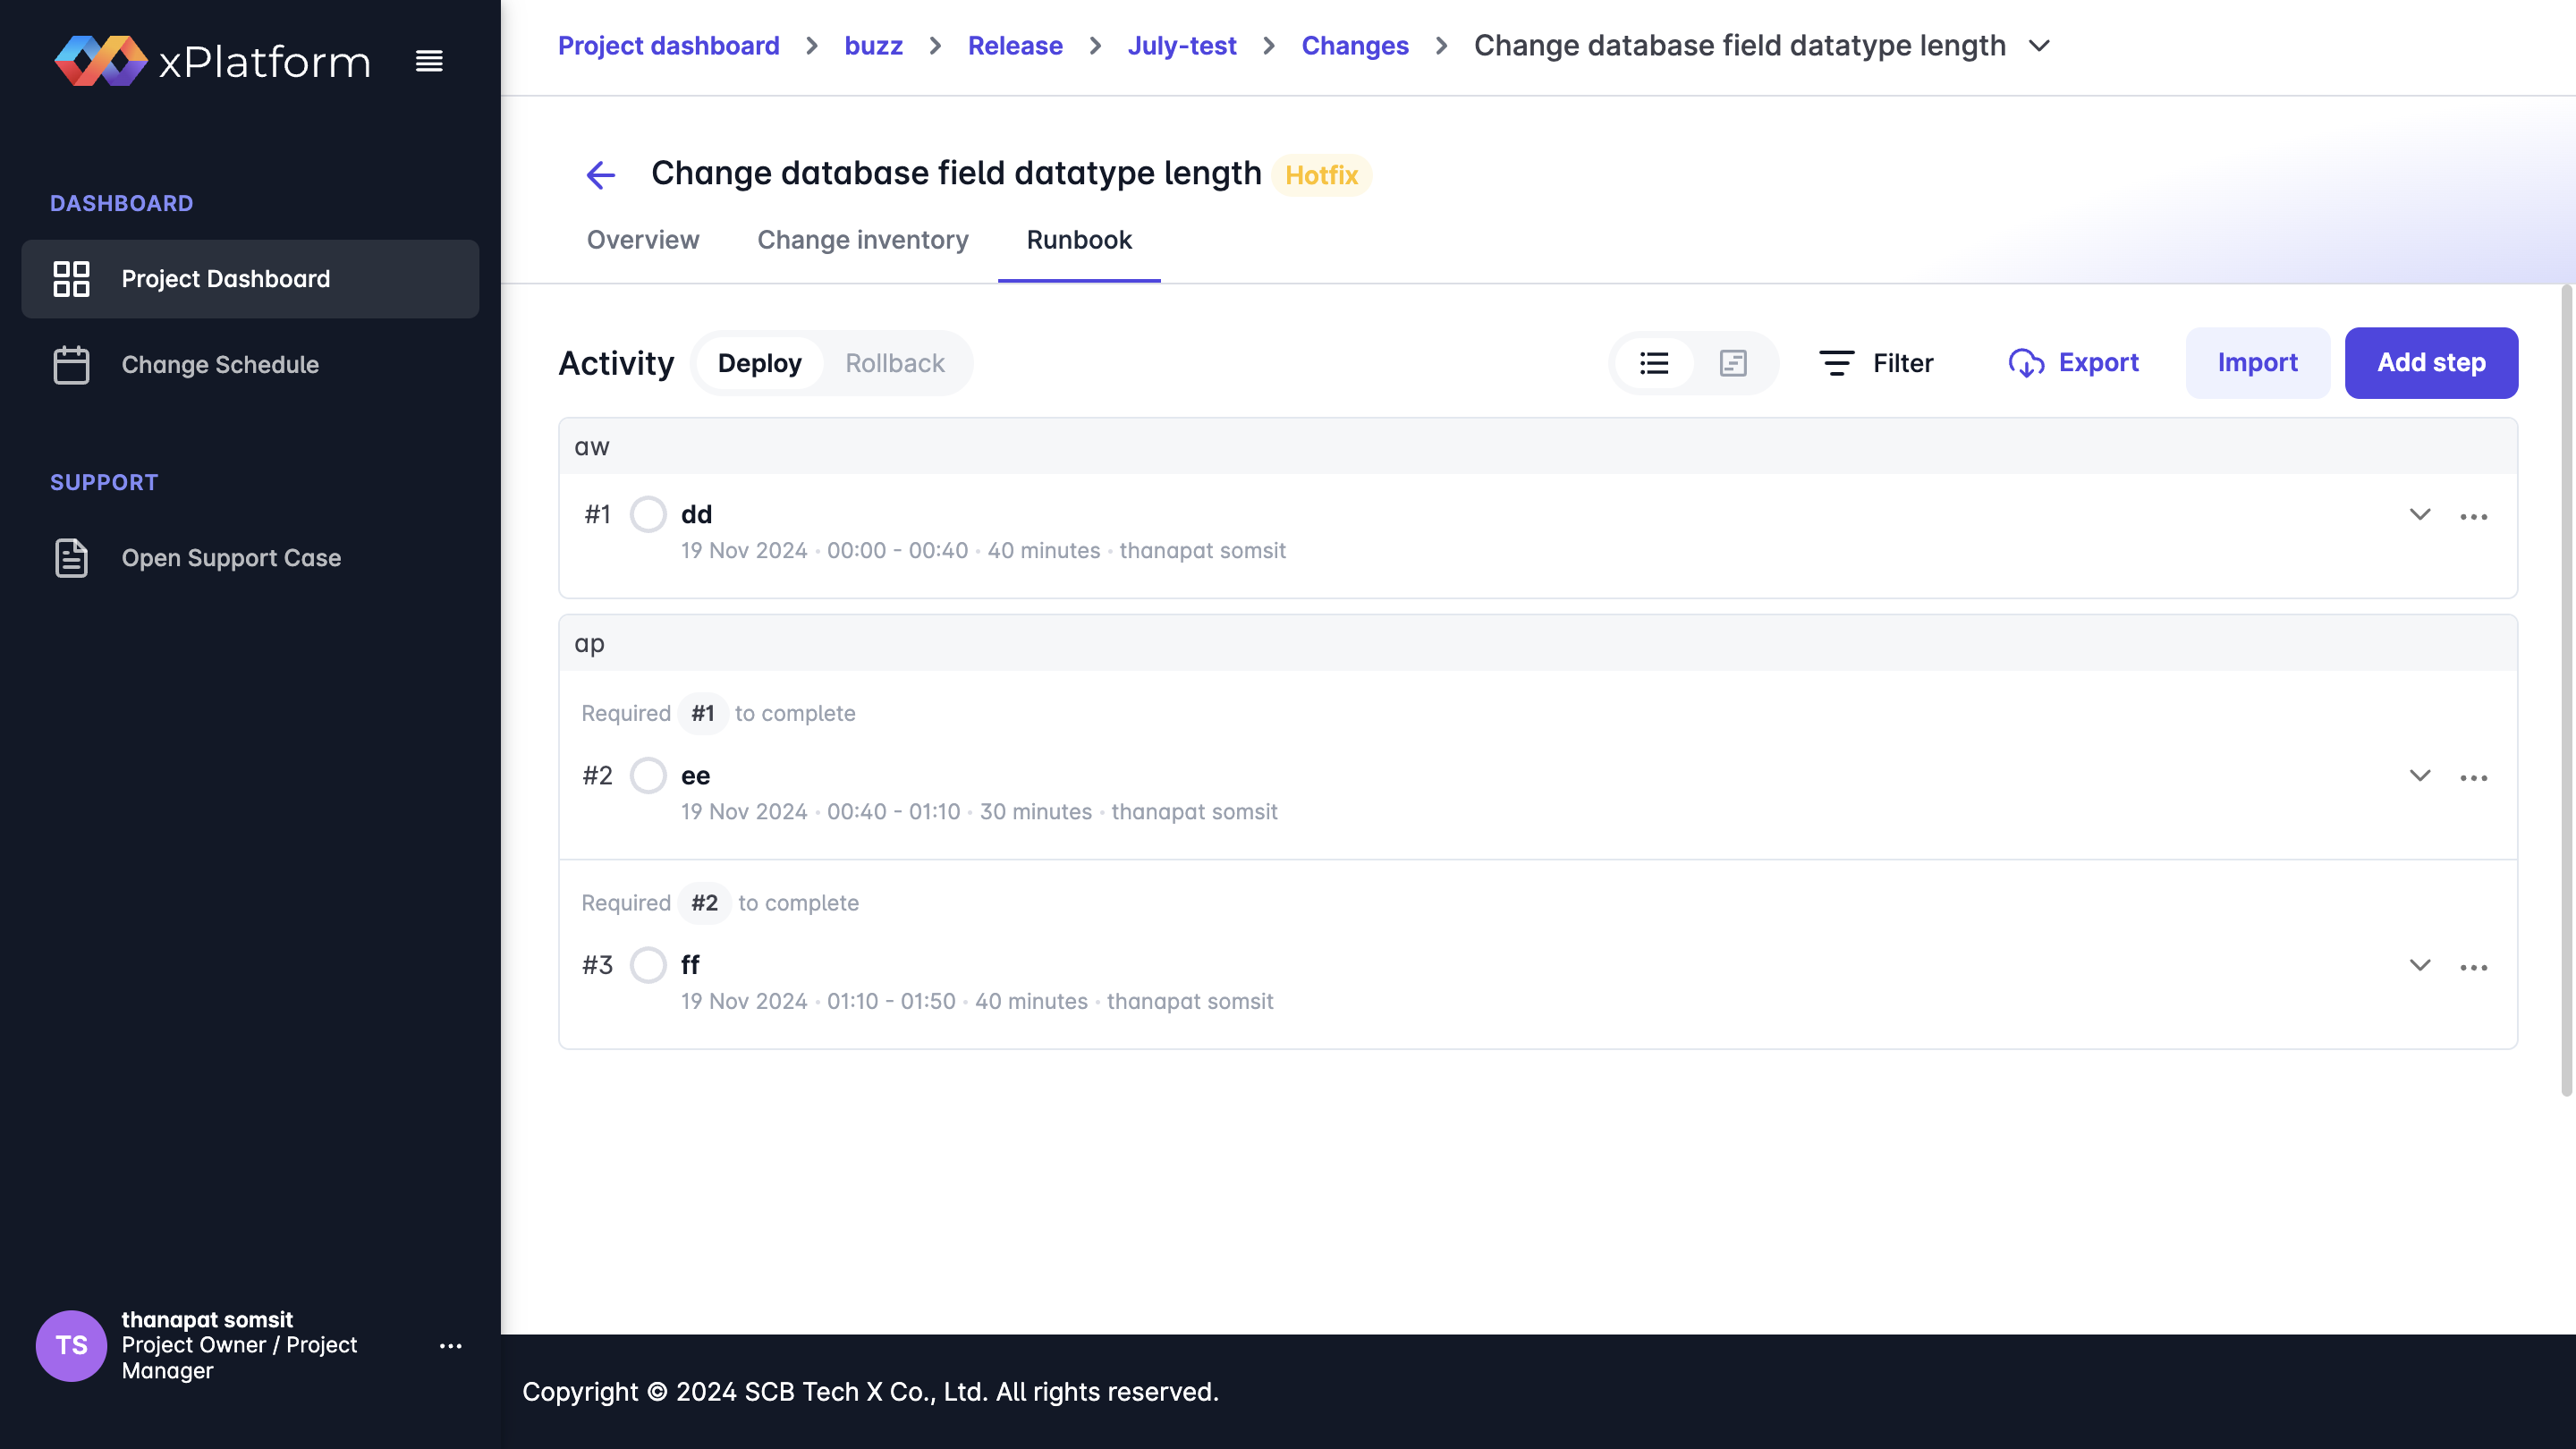
\includegraphics[width=\linewidth]{resources/pages/change-runbook/update-activity/10.png}
\end{center}
\caption[การเปลี่ยนแปลง Activity]{การเปลี่ยนแปลง Activity}
\label{fig:update-activity}
\end{figure}

\newpage
\subsection{การลบ Activity}
\begin{center}
    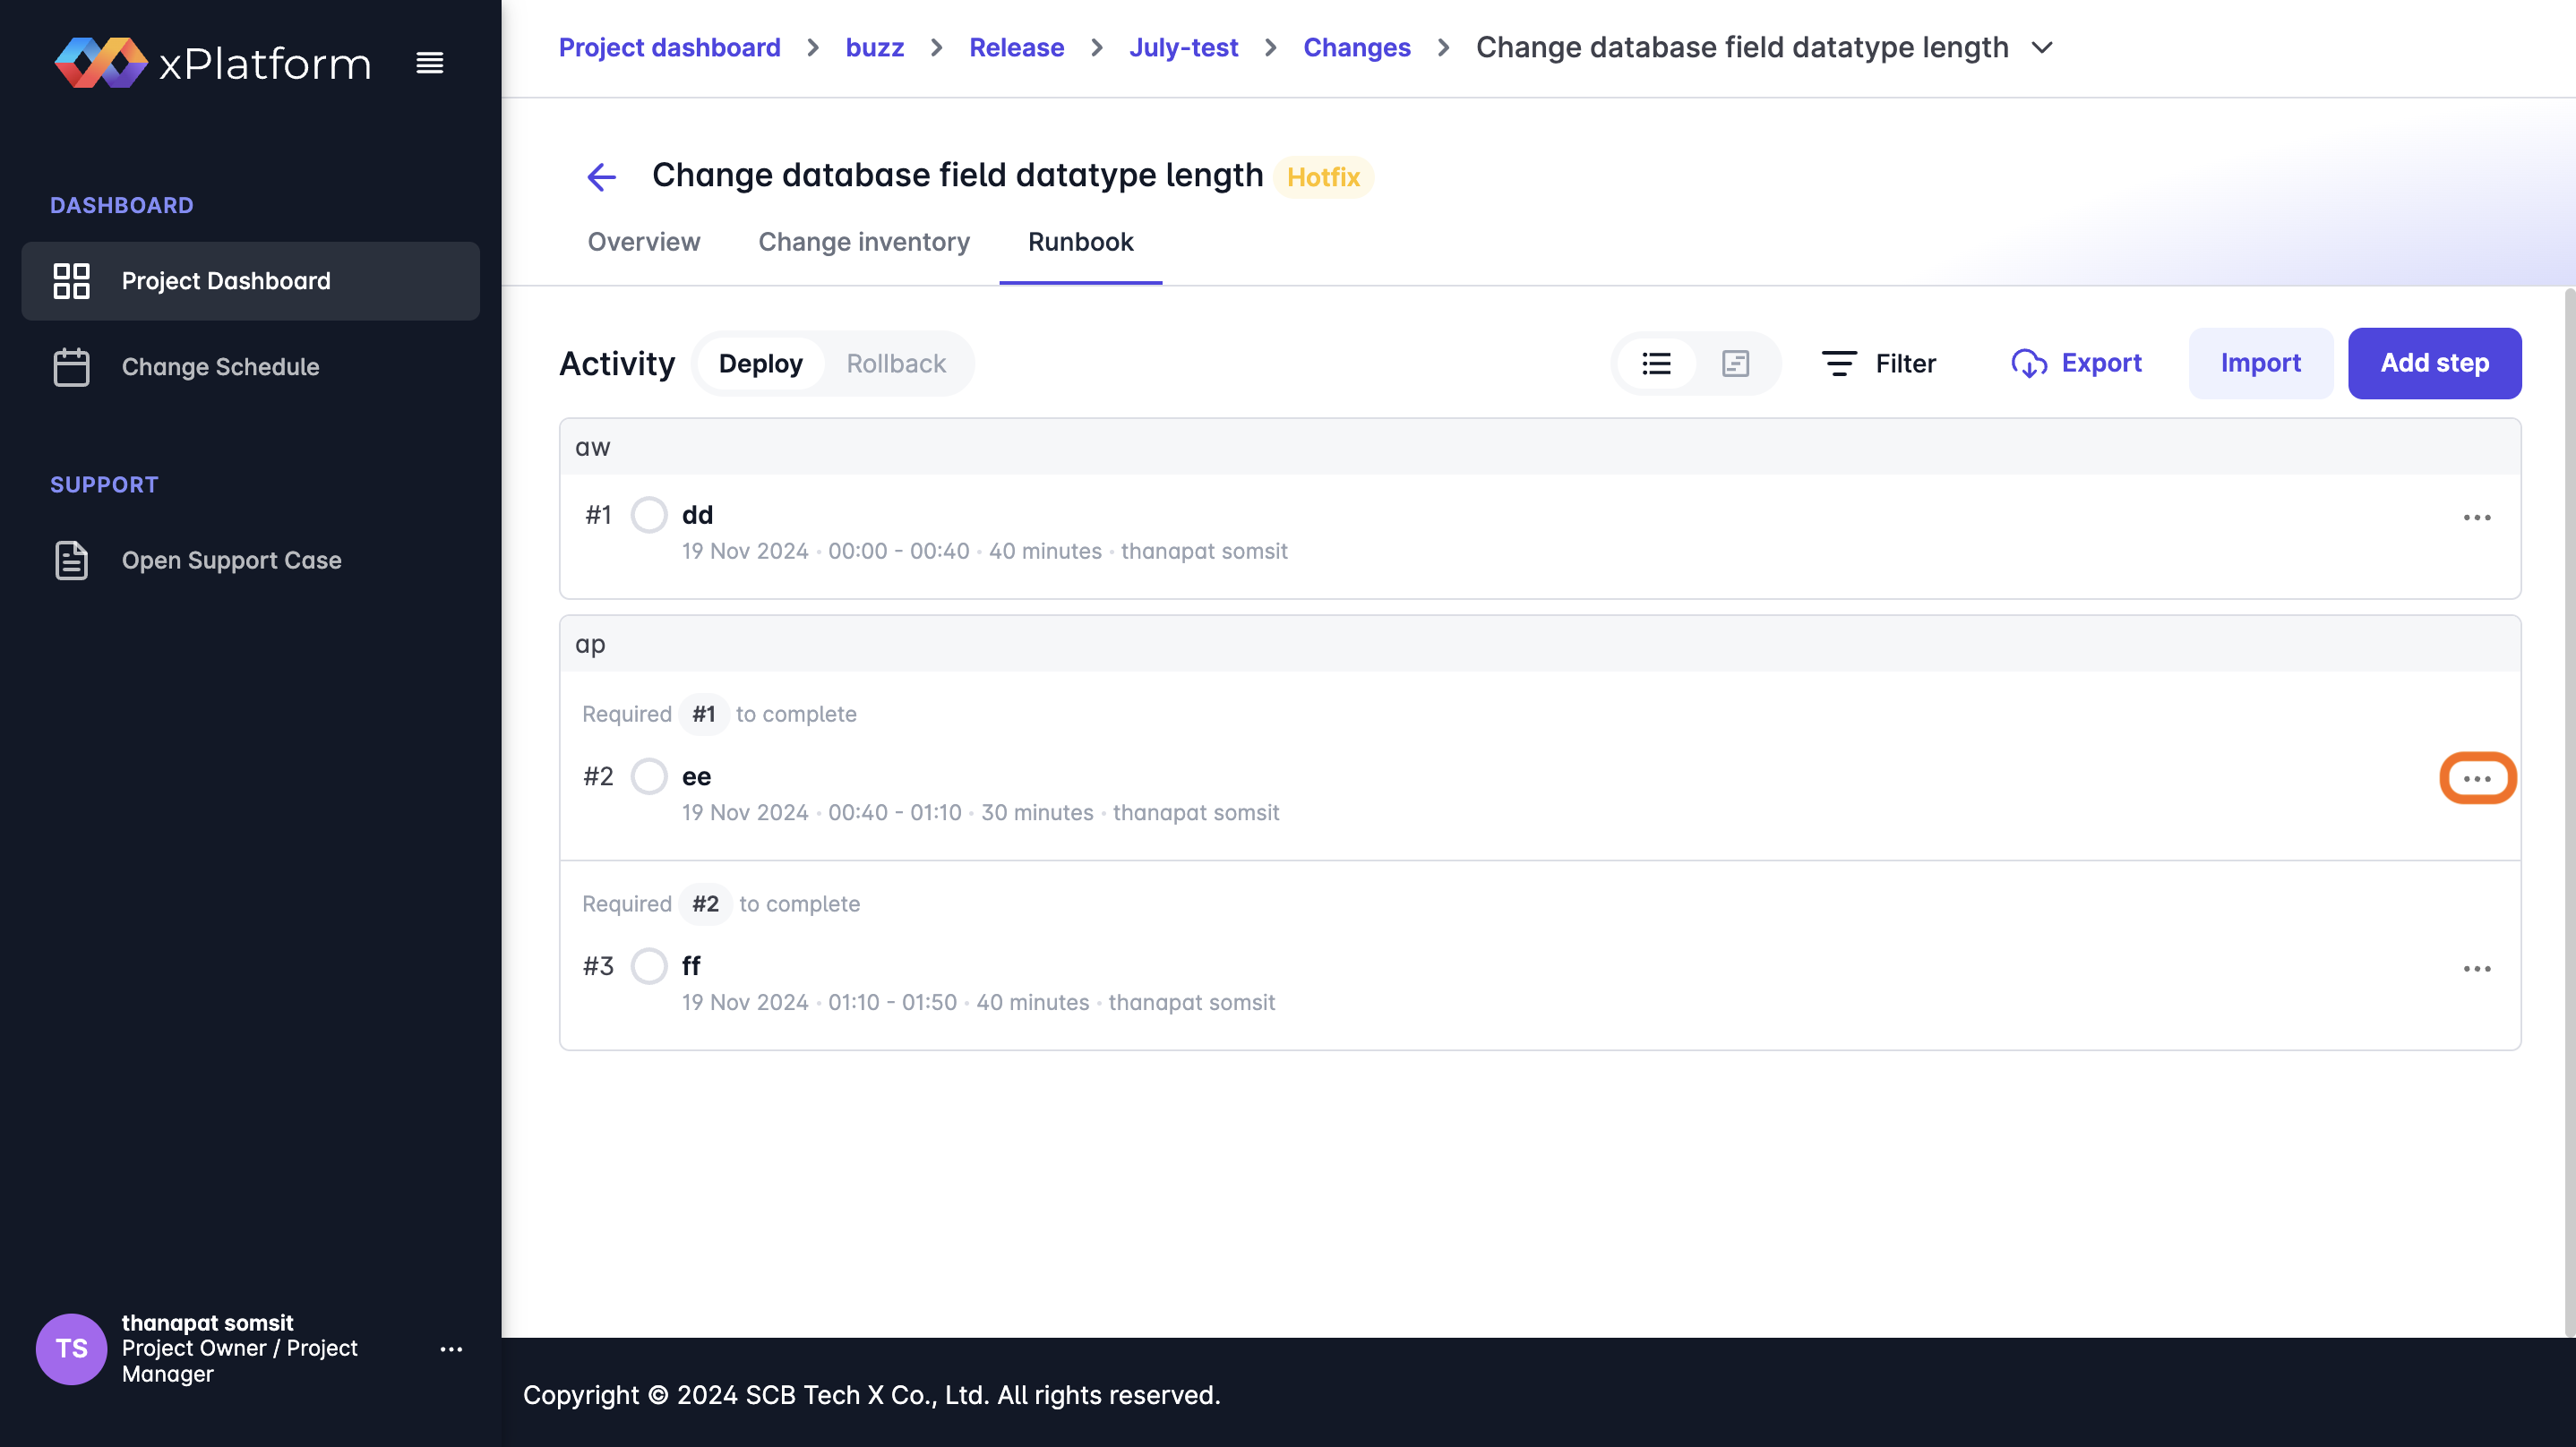
\includegraphics[width=\linewidth]{resources/pages/change-runbook/delete-activity/41.png}
    
    \vspace{1in}
    
    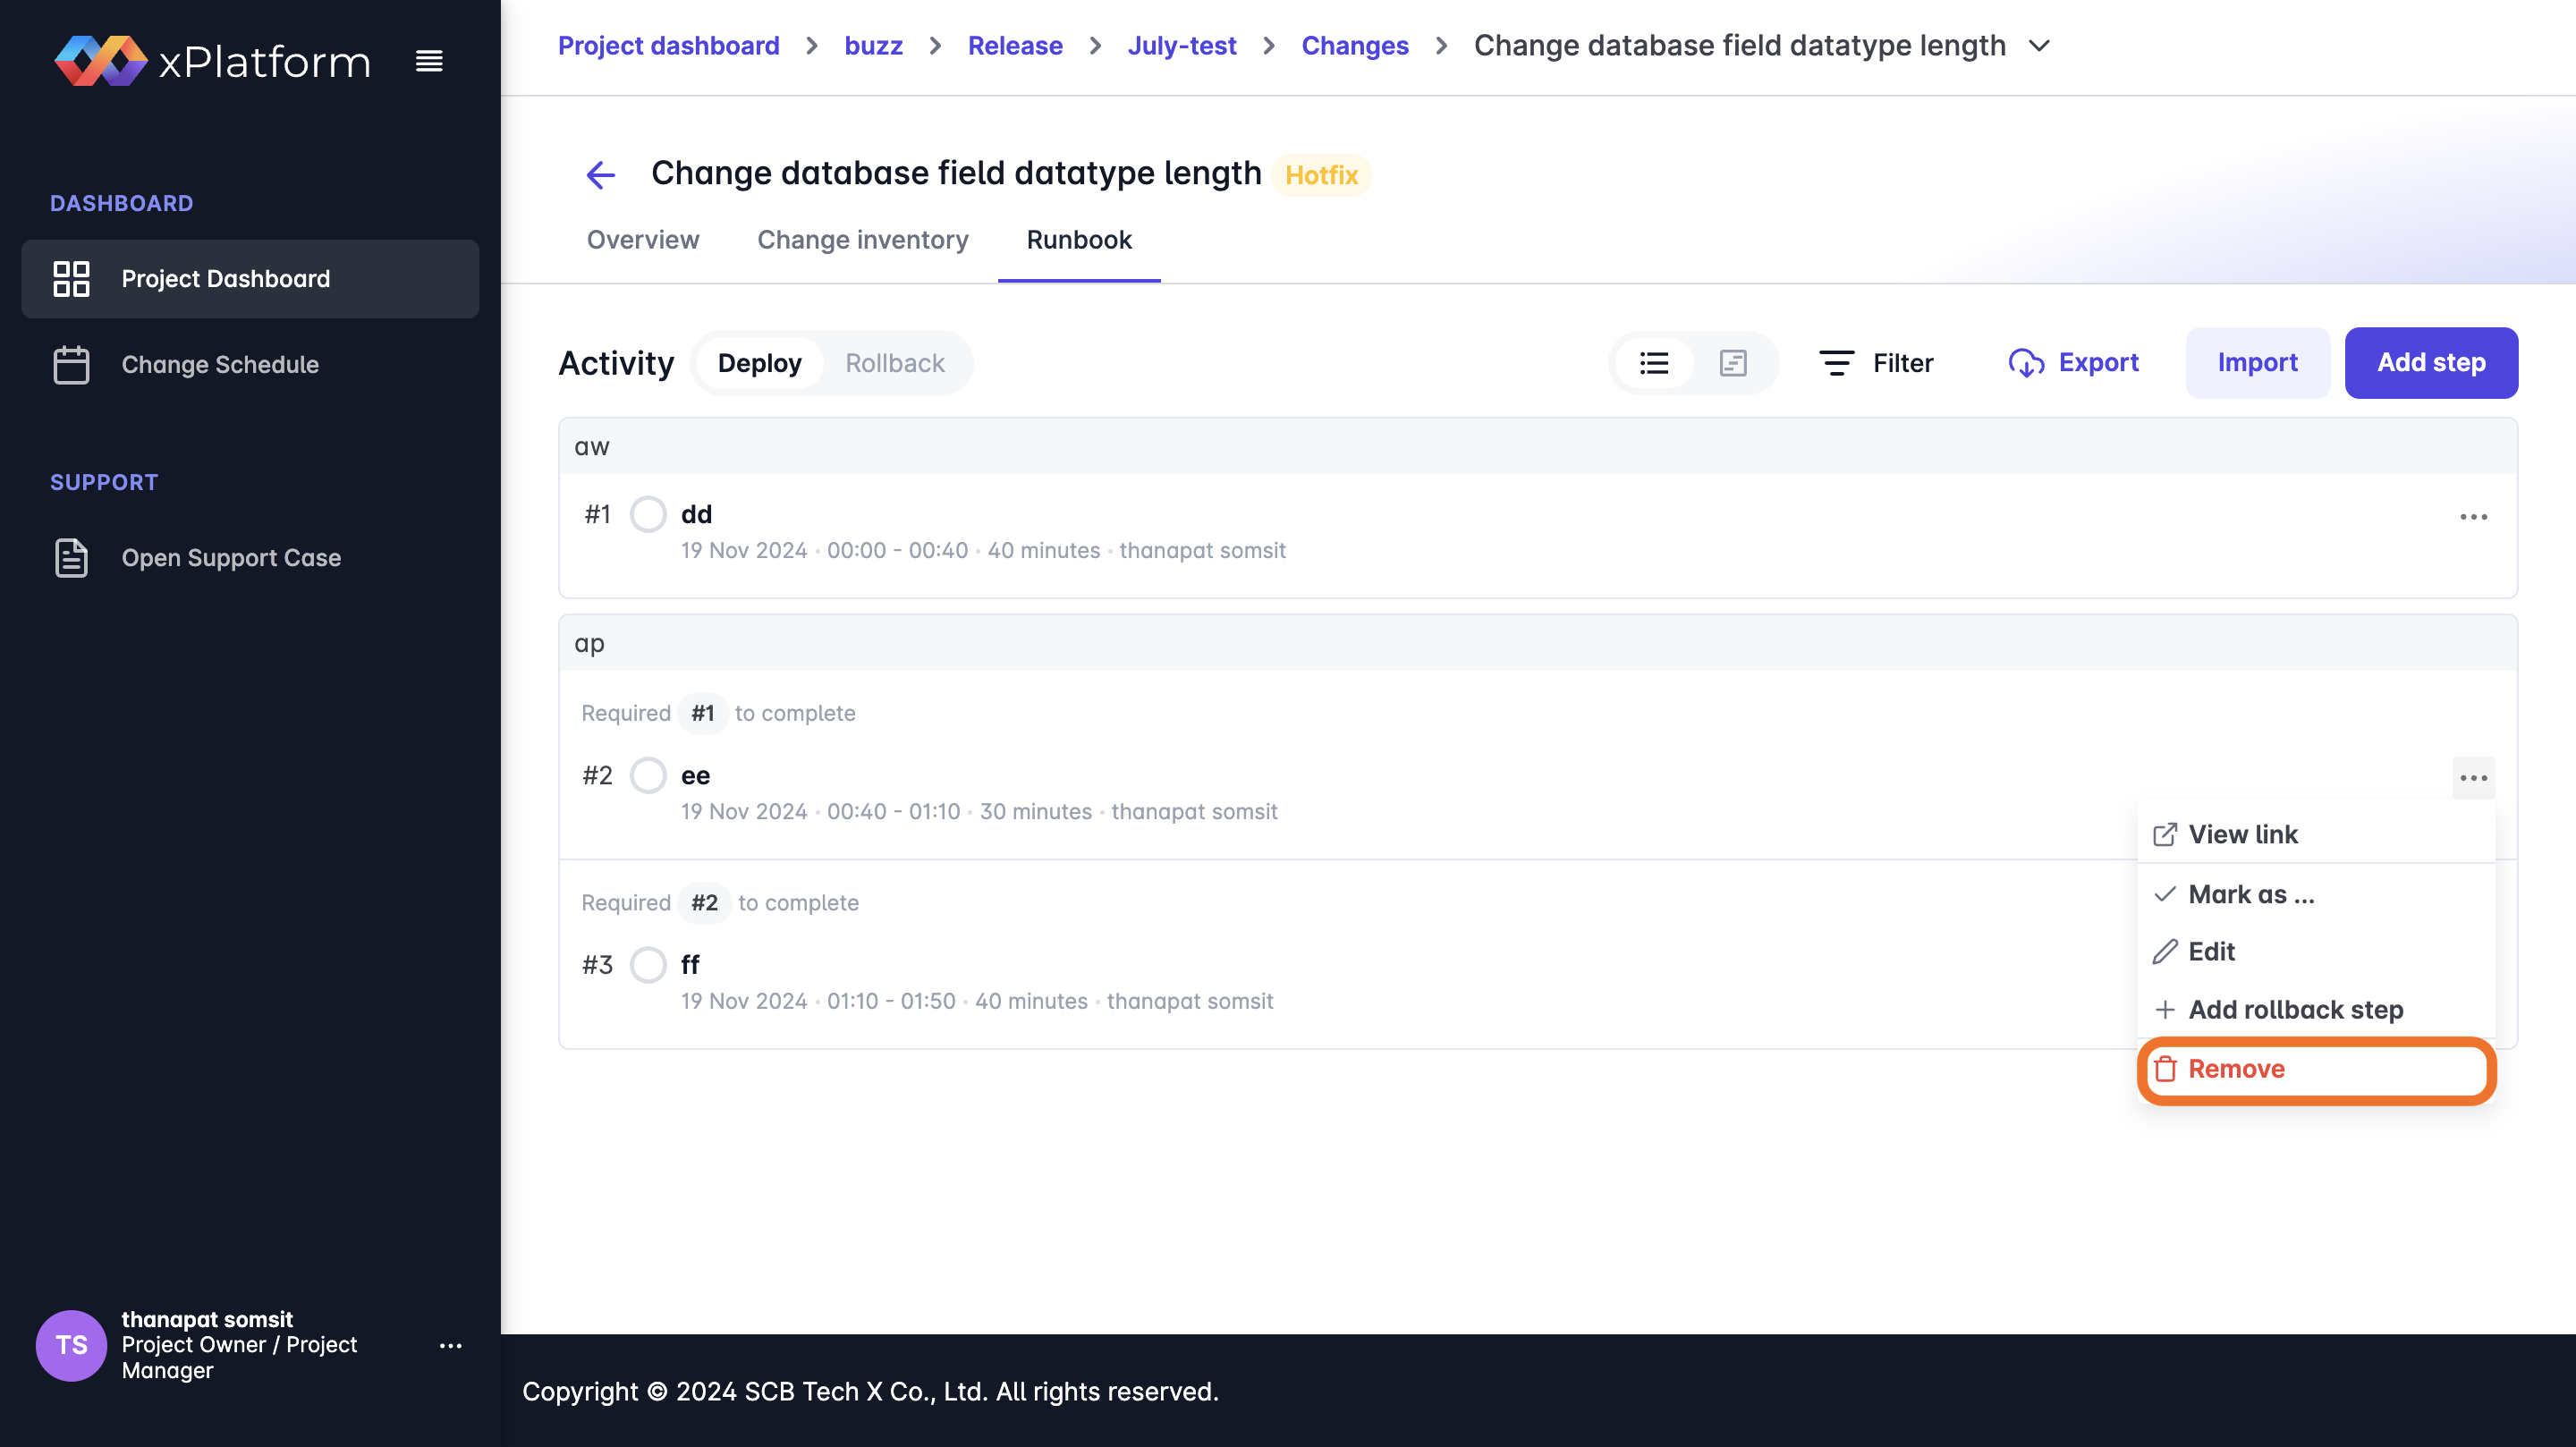
\includegraphics[width=\linewidth]{resources/pages/change-runbook/delete-activity/42.png}
\end{center}
    
\begin{figure}[H]
\begin{center}
    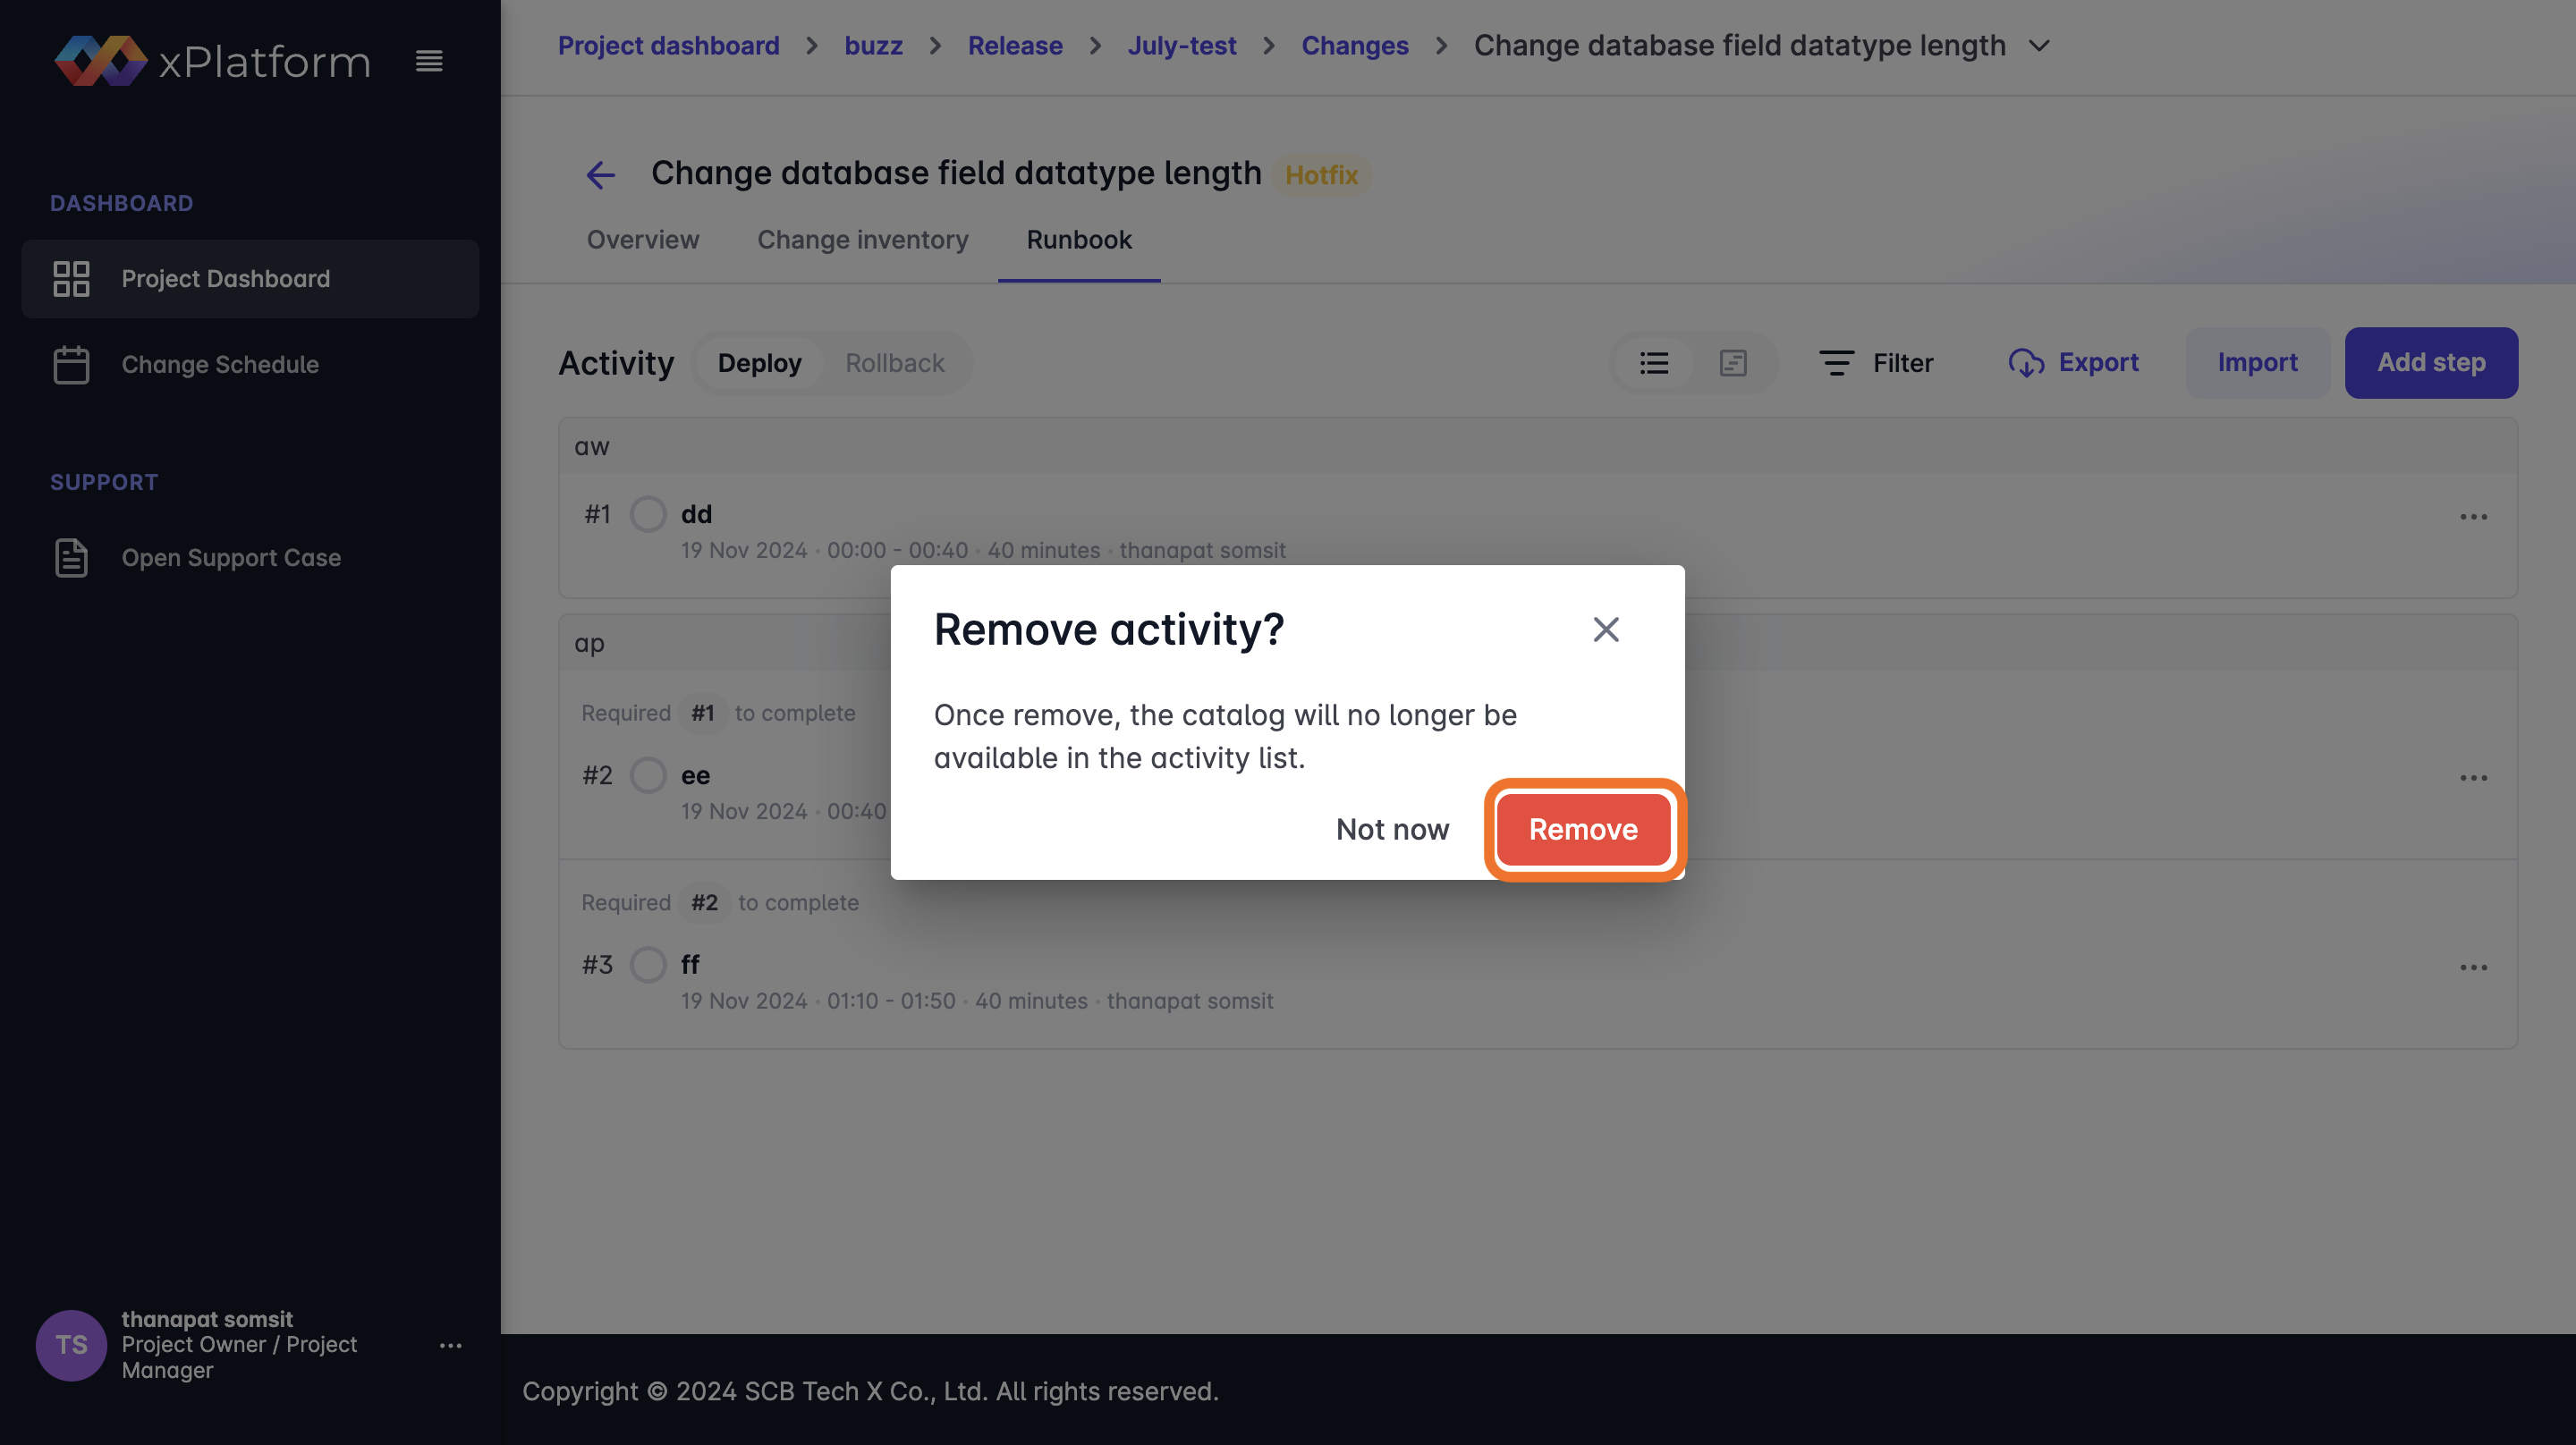
\includegraphics[width=\linewidth]{resources/pages/change-runbook/delete-activity/43.png}

    \vspace{1in}

    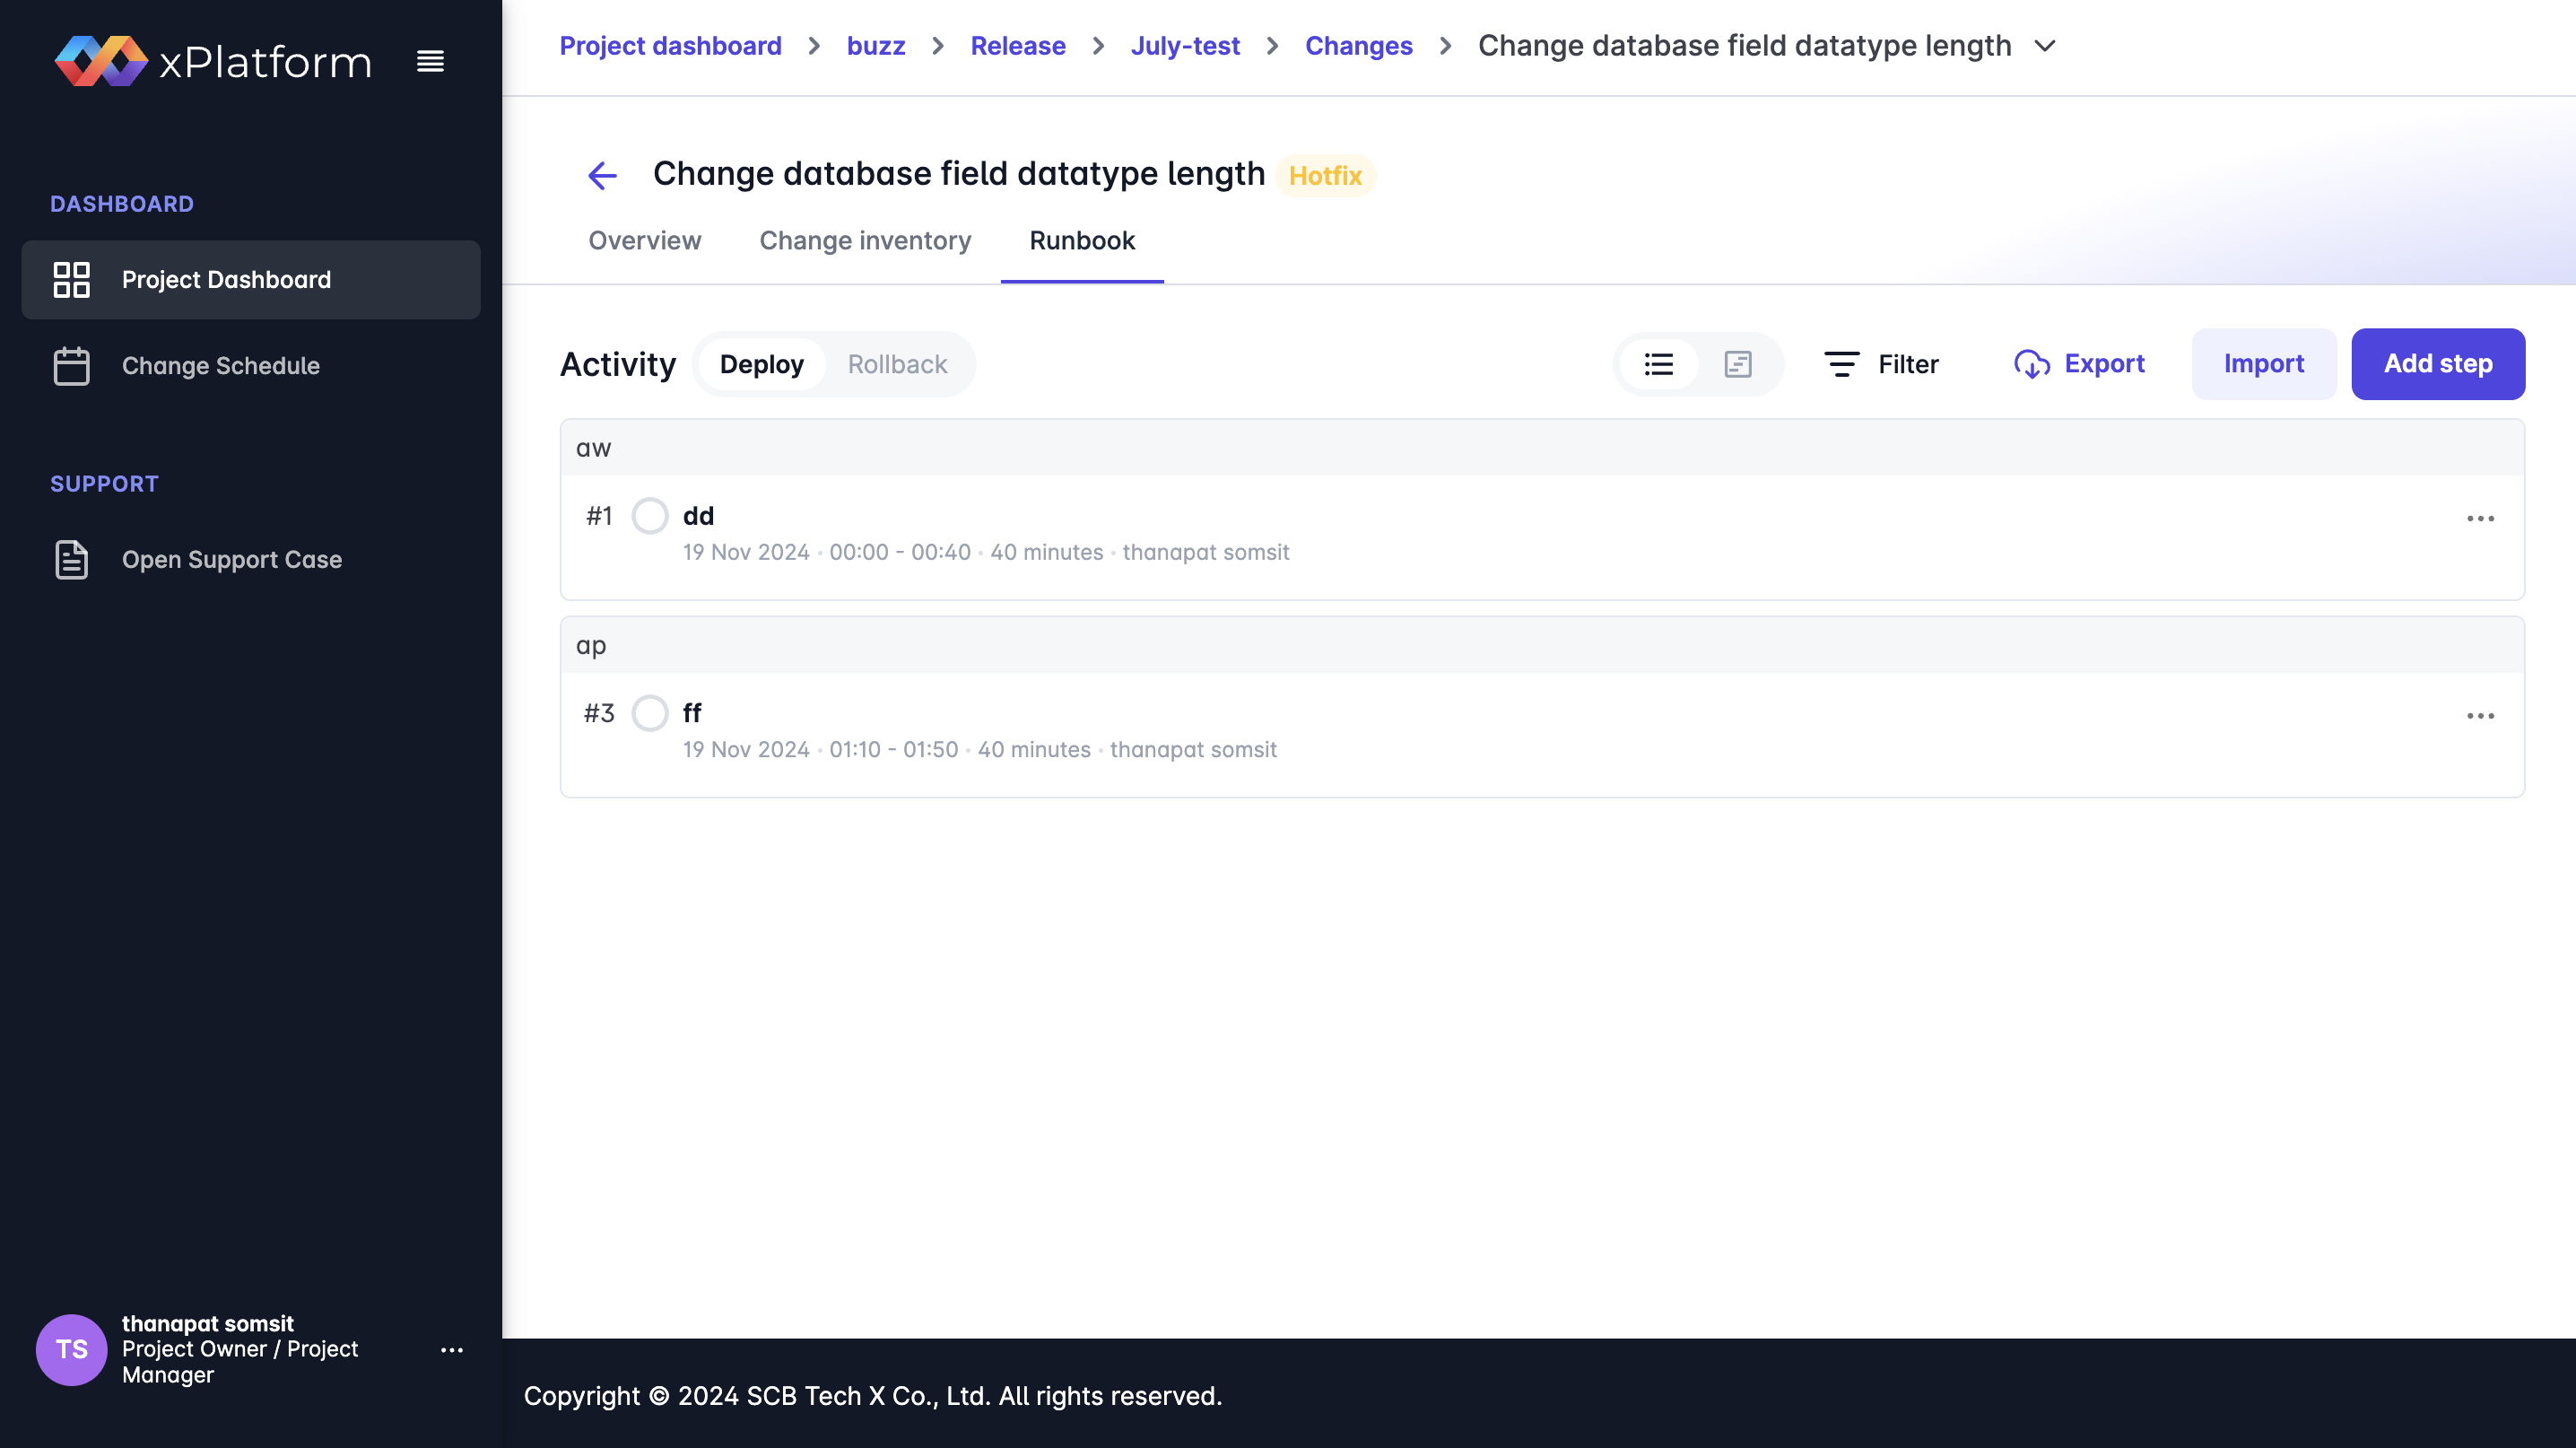
\includegraphics[width=\linewidth]{resources/pages/change-runbook/delete-activity/44.png}
\end{center}
\caption[การลบ Activity]{การลบ Activity}
\label{fig:delete-activity}
\end{figure}

\newpage
\subsection{การ Mark Activity}
\begin{center}
    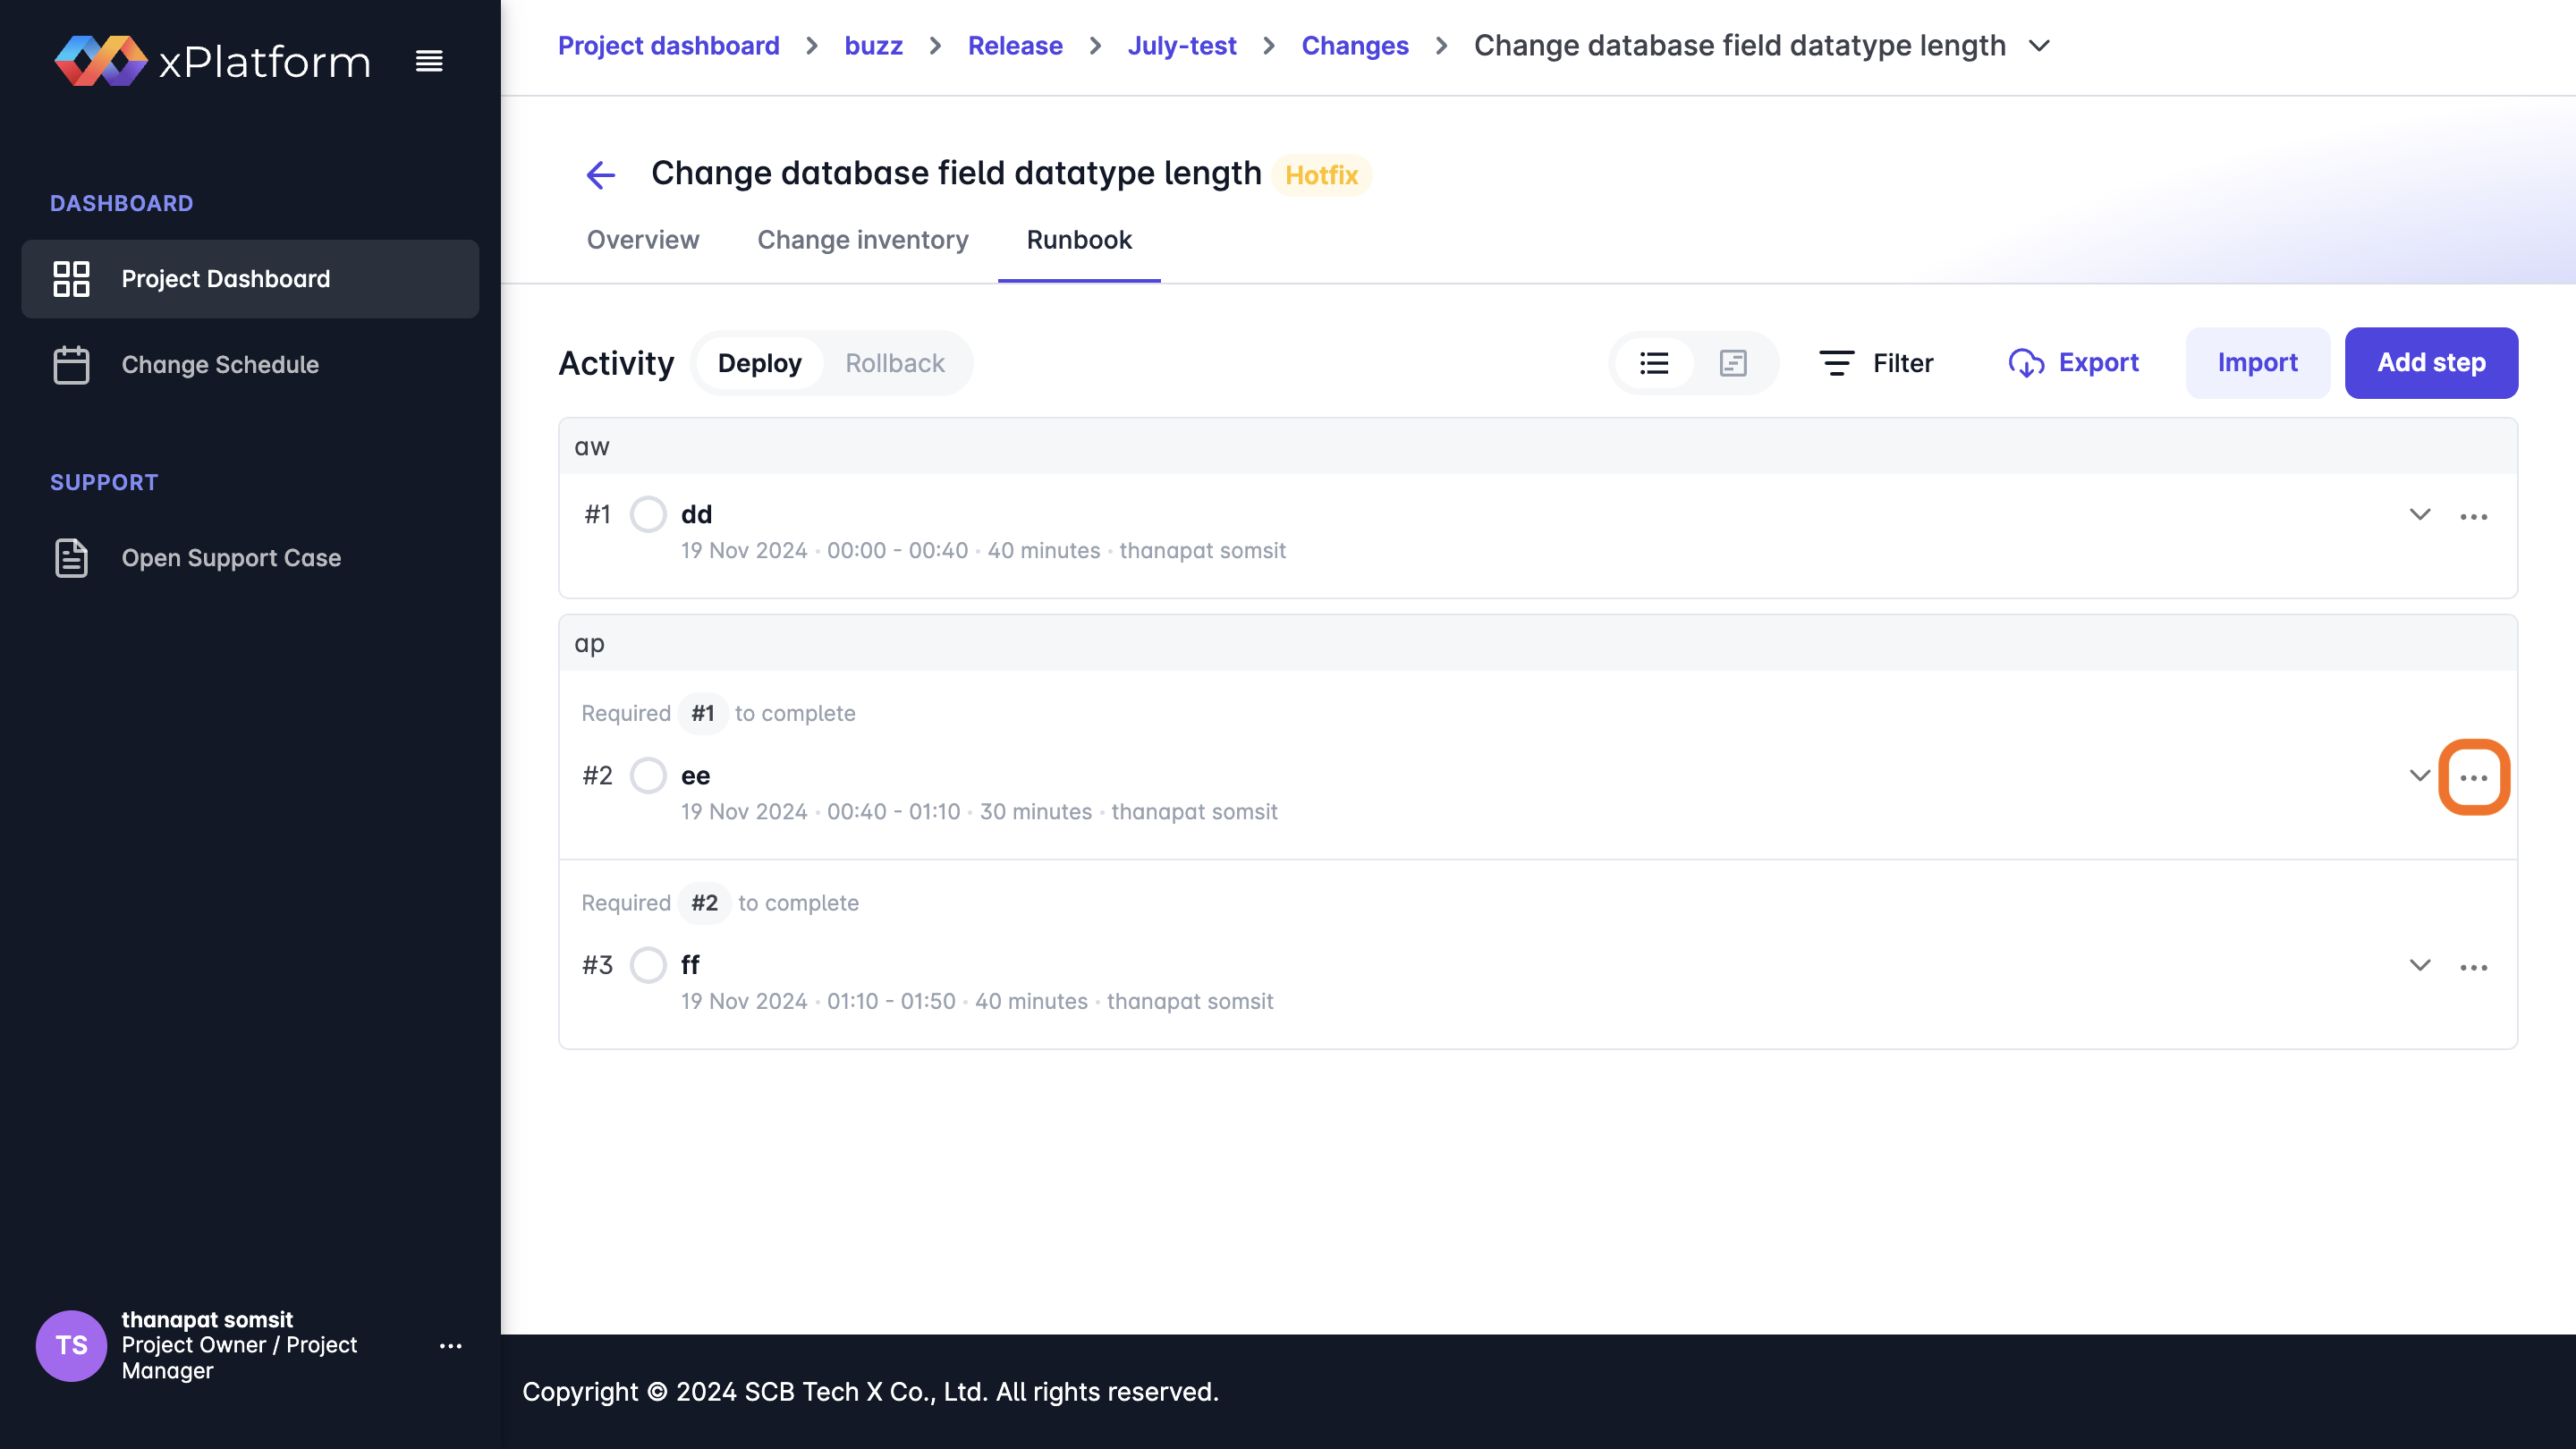
\includegraphics[width=\linewidth]{resources/pages/change-runbook/mark-activity/13.png}
    
    \vspace{1in}
    
    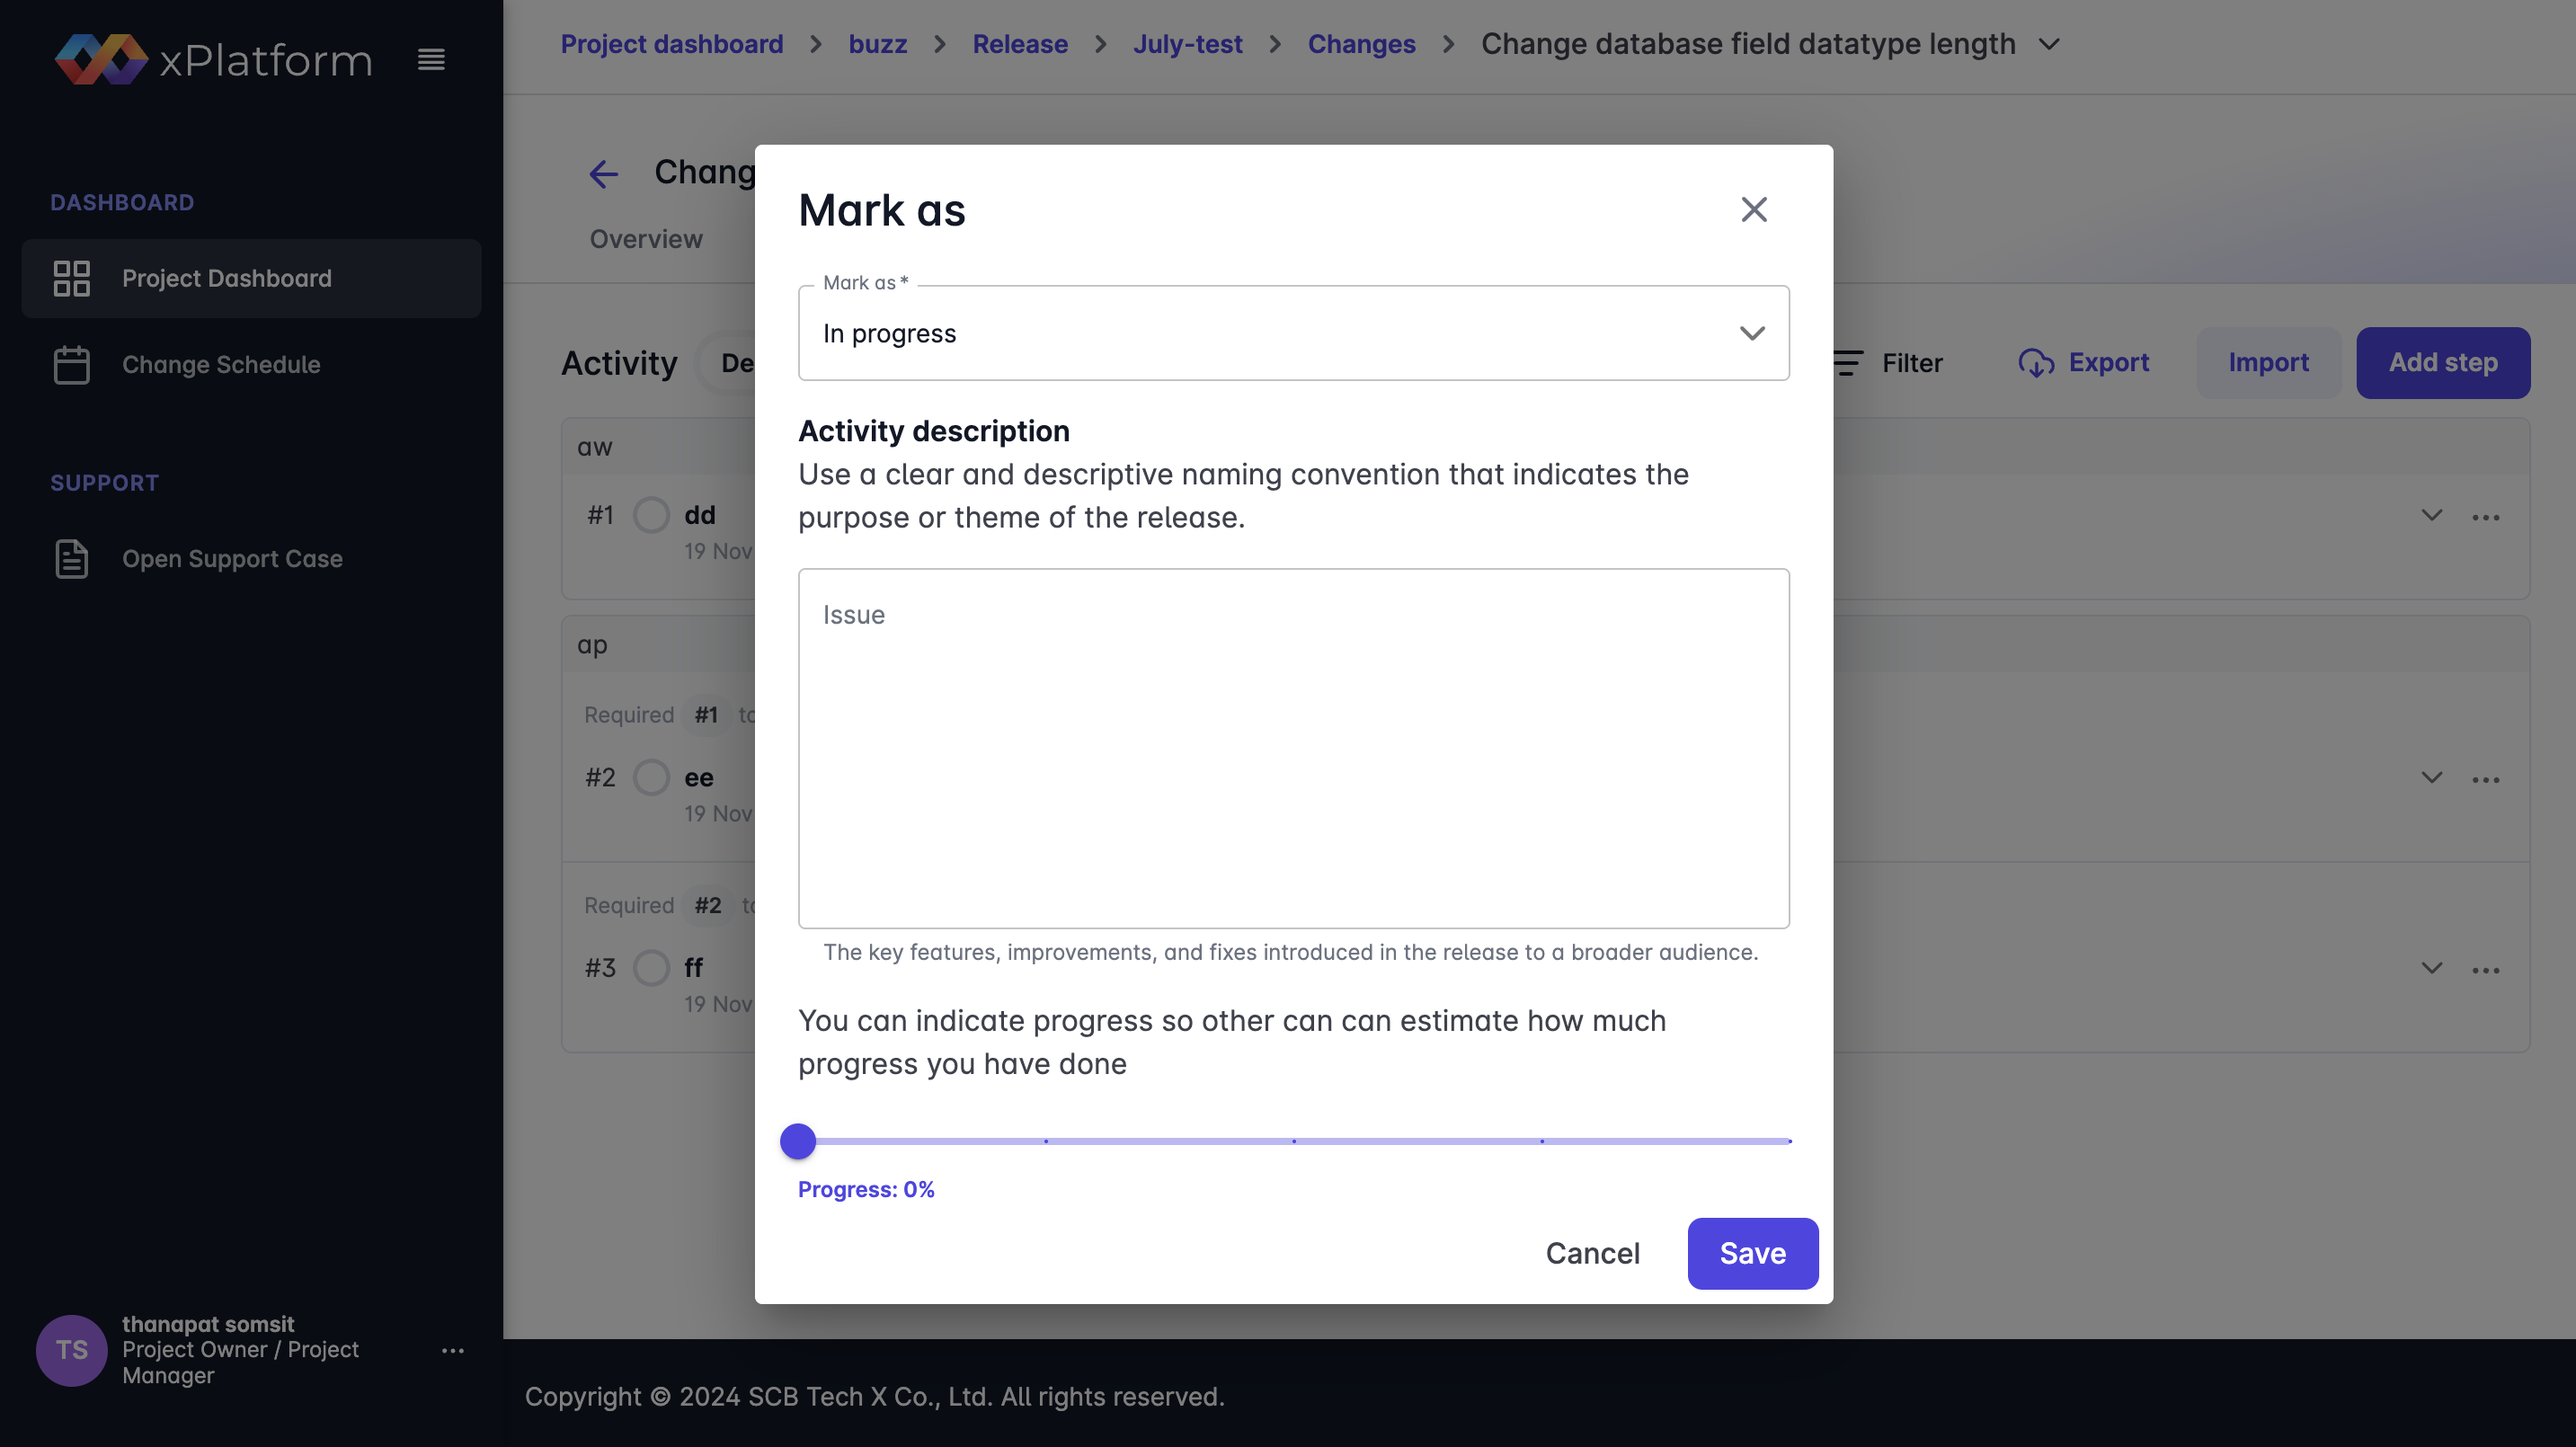
\includegraphics[width=\linewidth]{resources/pages/change-runbook/mark-activity/14.png}
\end{center}
    
\begin{figure}[H]
\begin{center}
    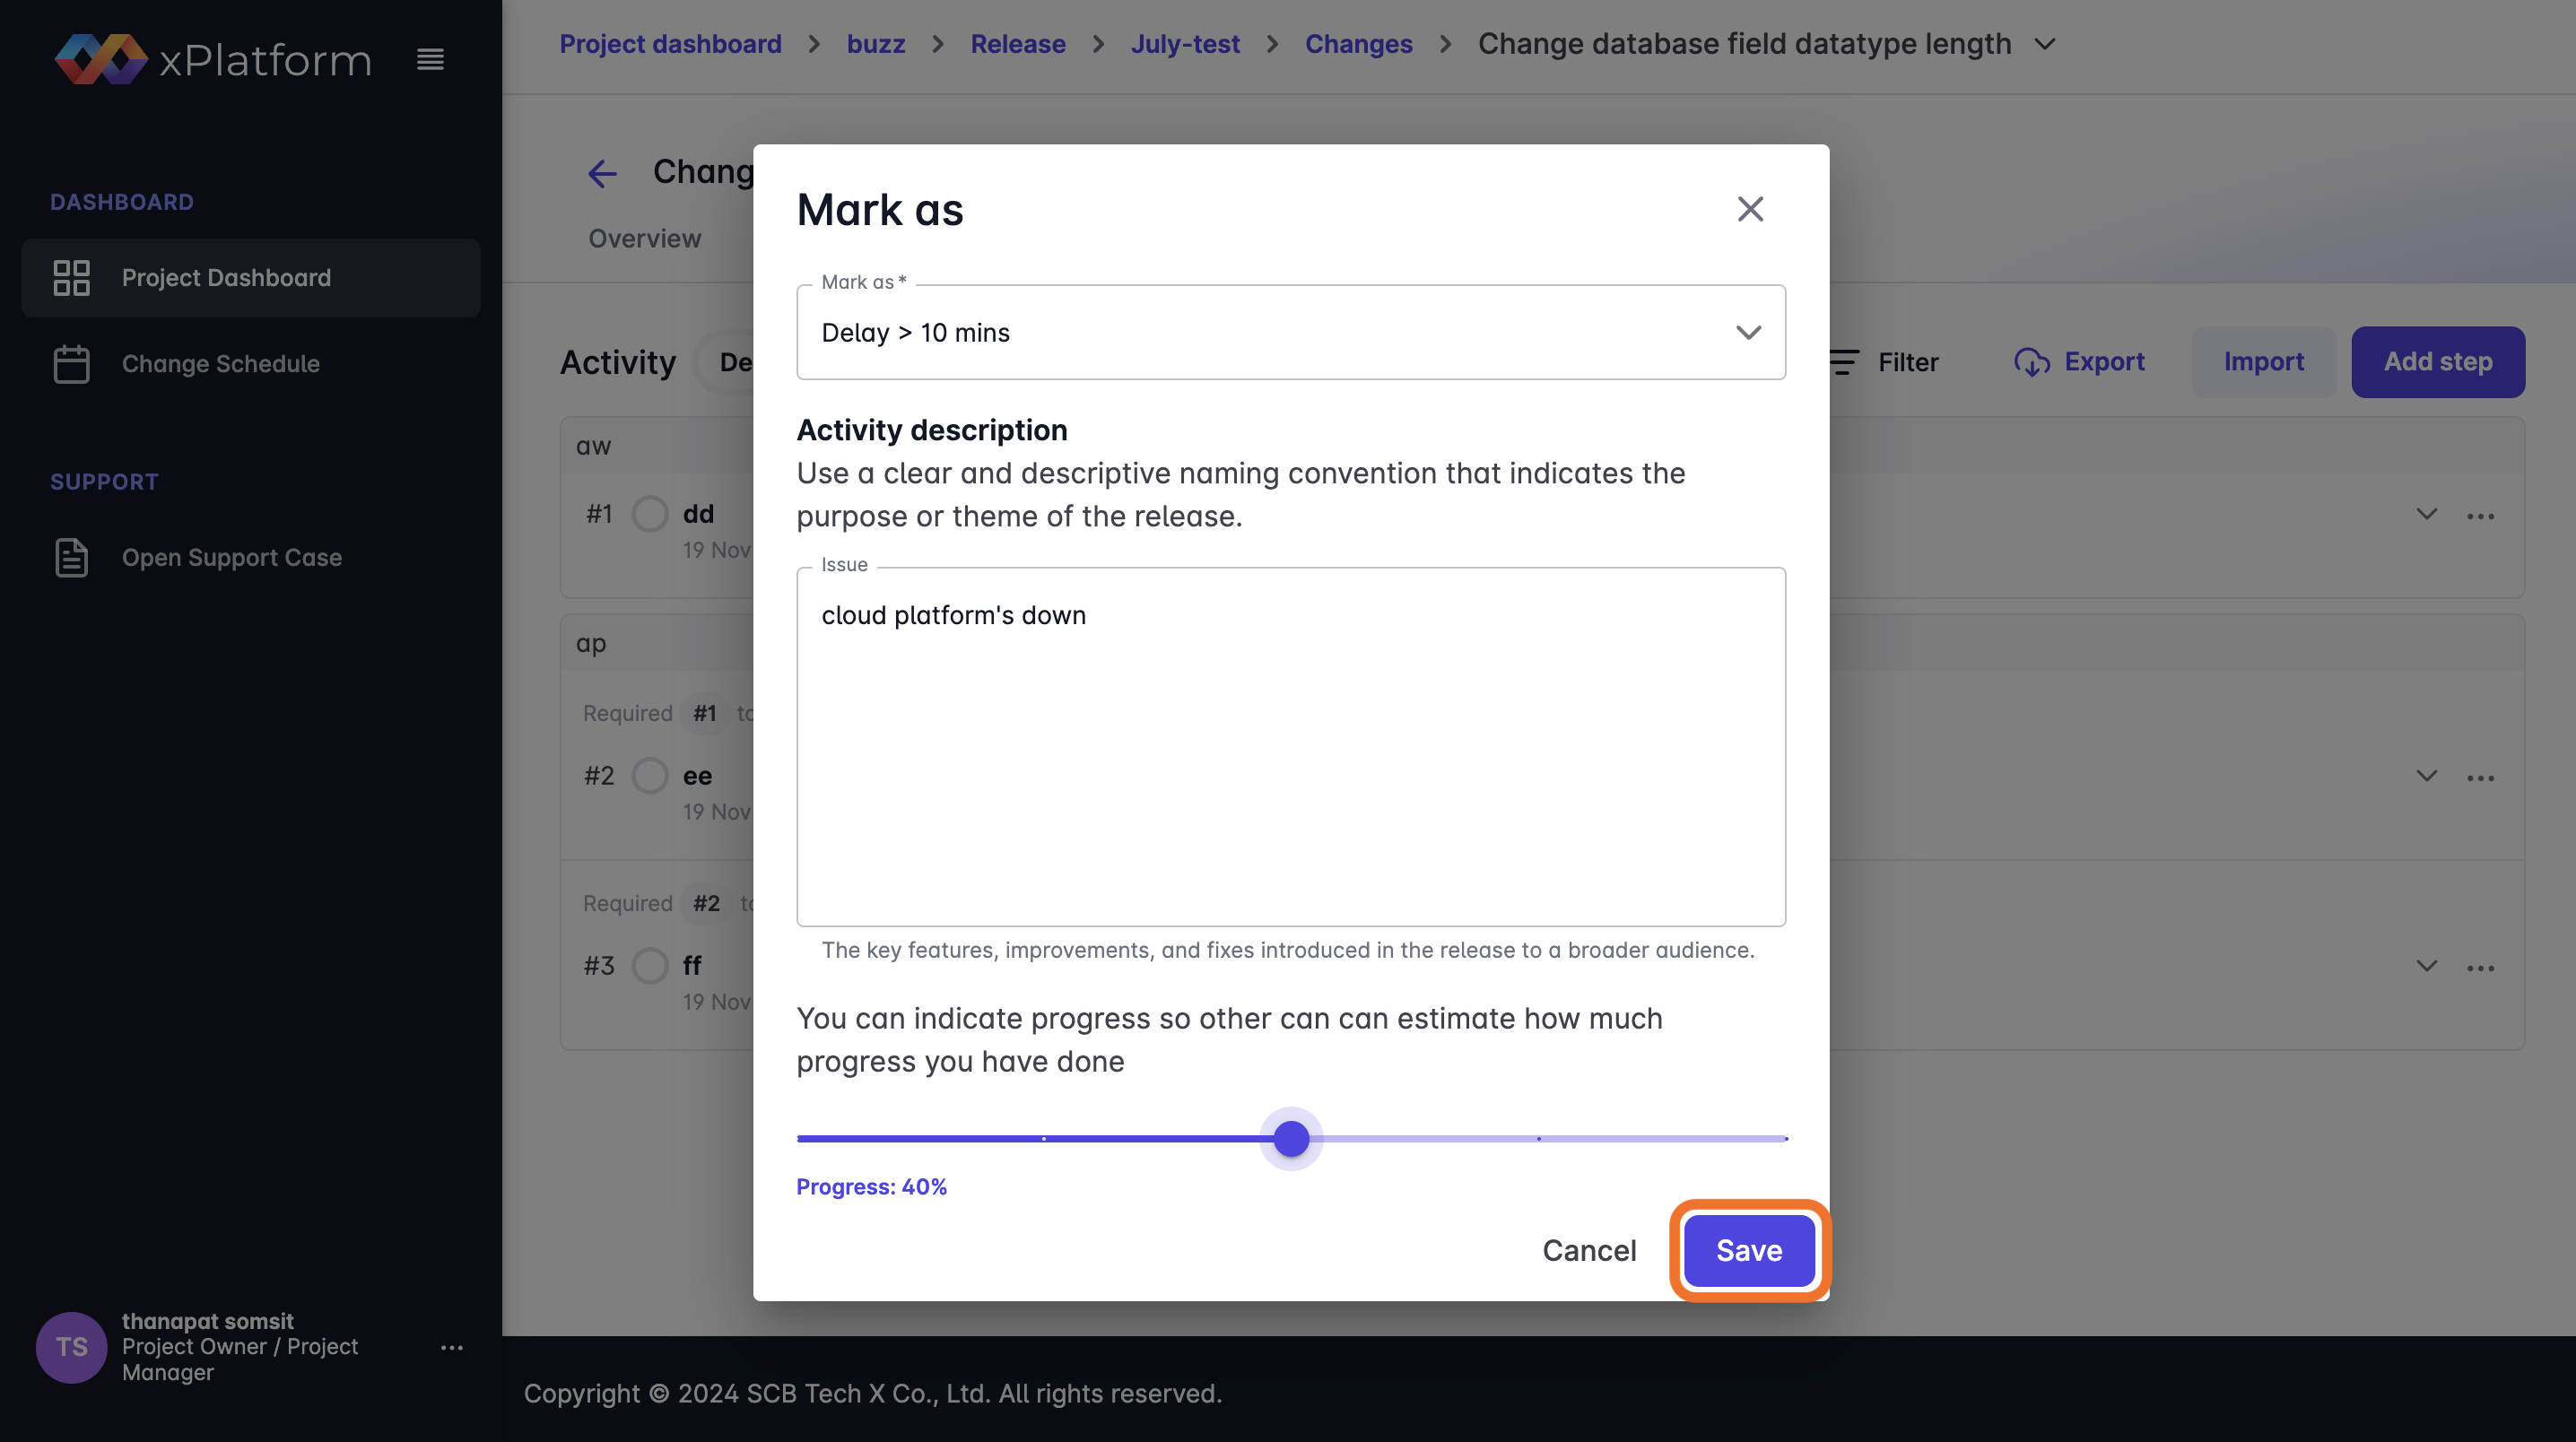
\includegraphics[width=\linewidth]{resources/pages/change-runbook/mark-activity/15.png}

    \vspace{1in}

    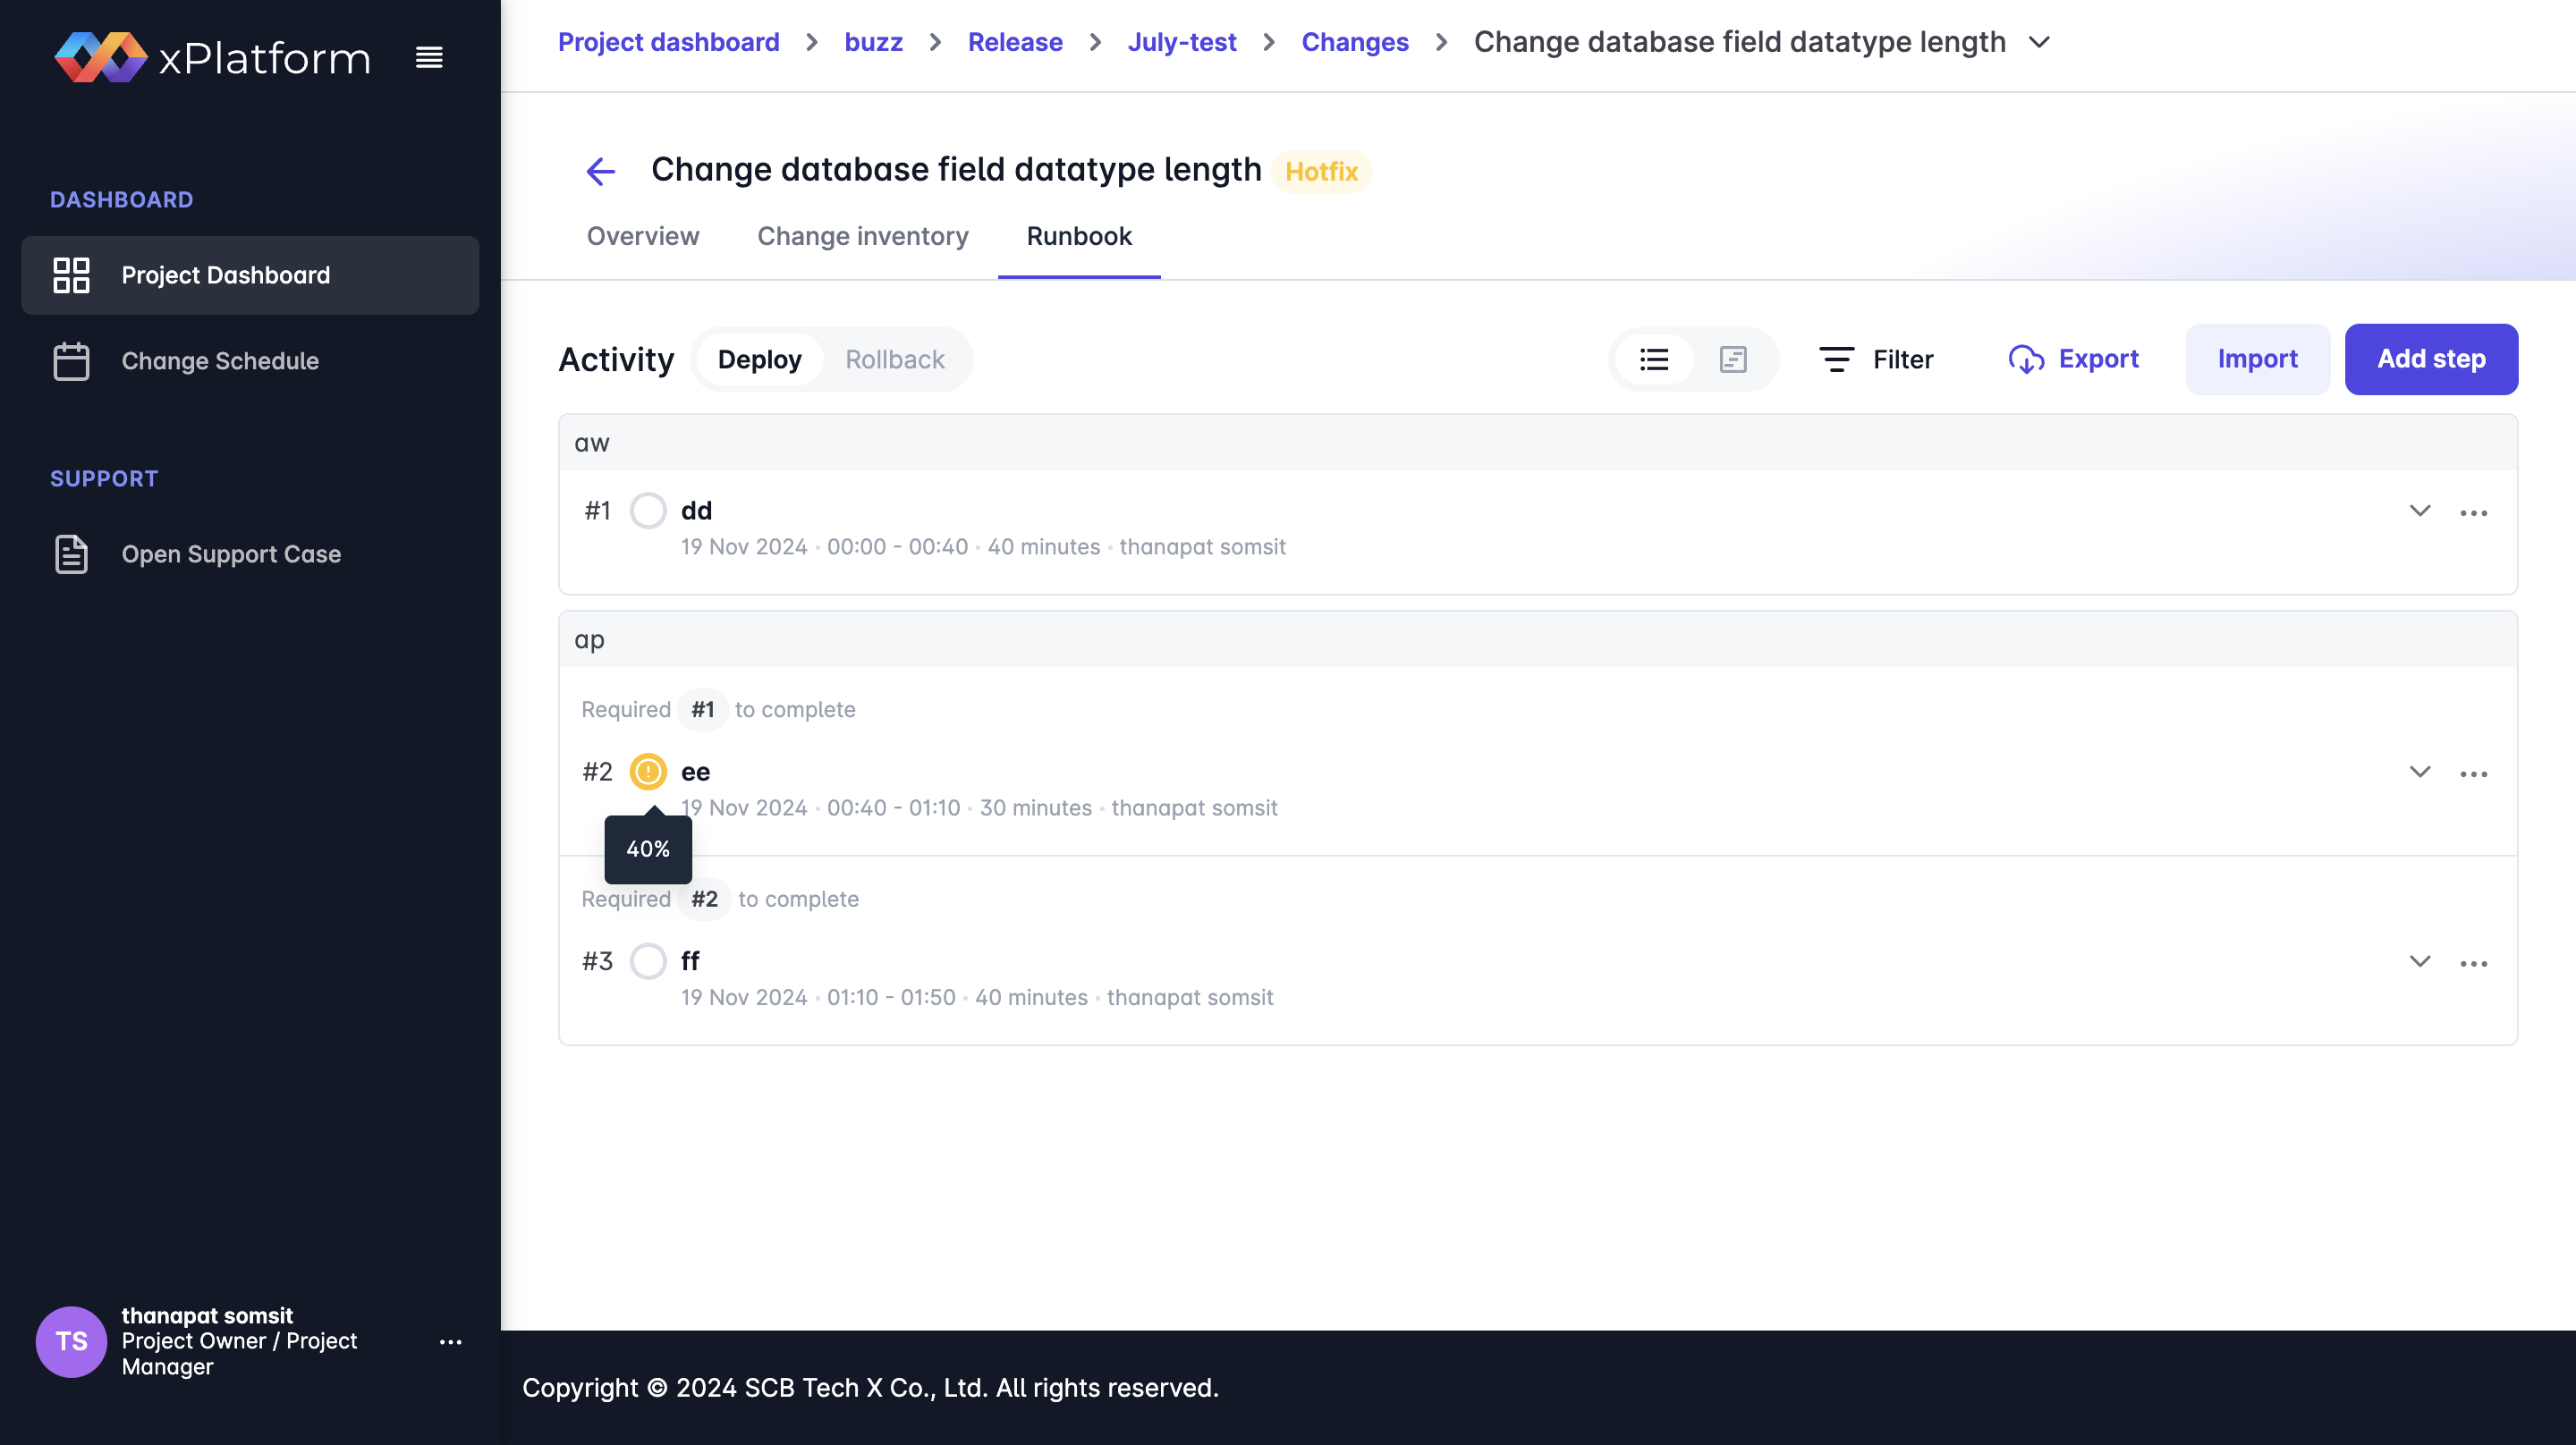
\includegraphics[width=\linewidth]{resources/pages/change-runbook/mark-activity/16.png}
\end{center}
\caption[การ Mark Activity]{การ Mark Activity}
\label{fig:mark-activity}
\end{figure}

\newpage
\subsection{การดึงข้อมูลจาก Jira}
\begin{center}
    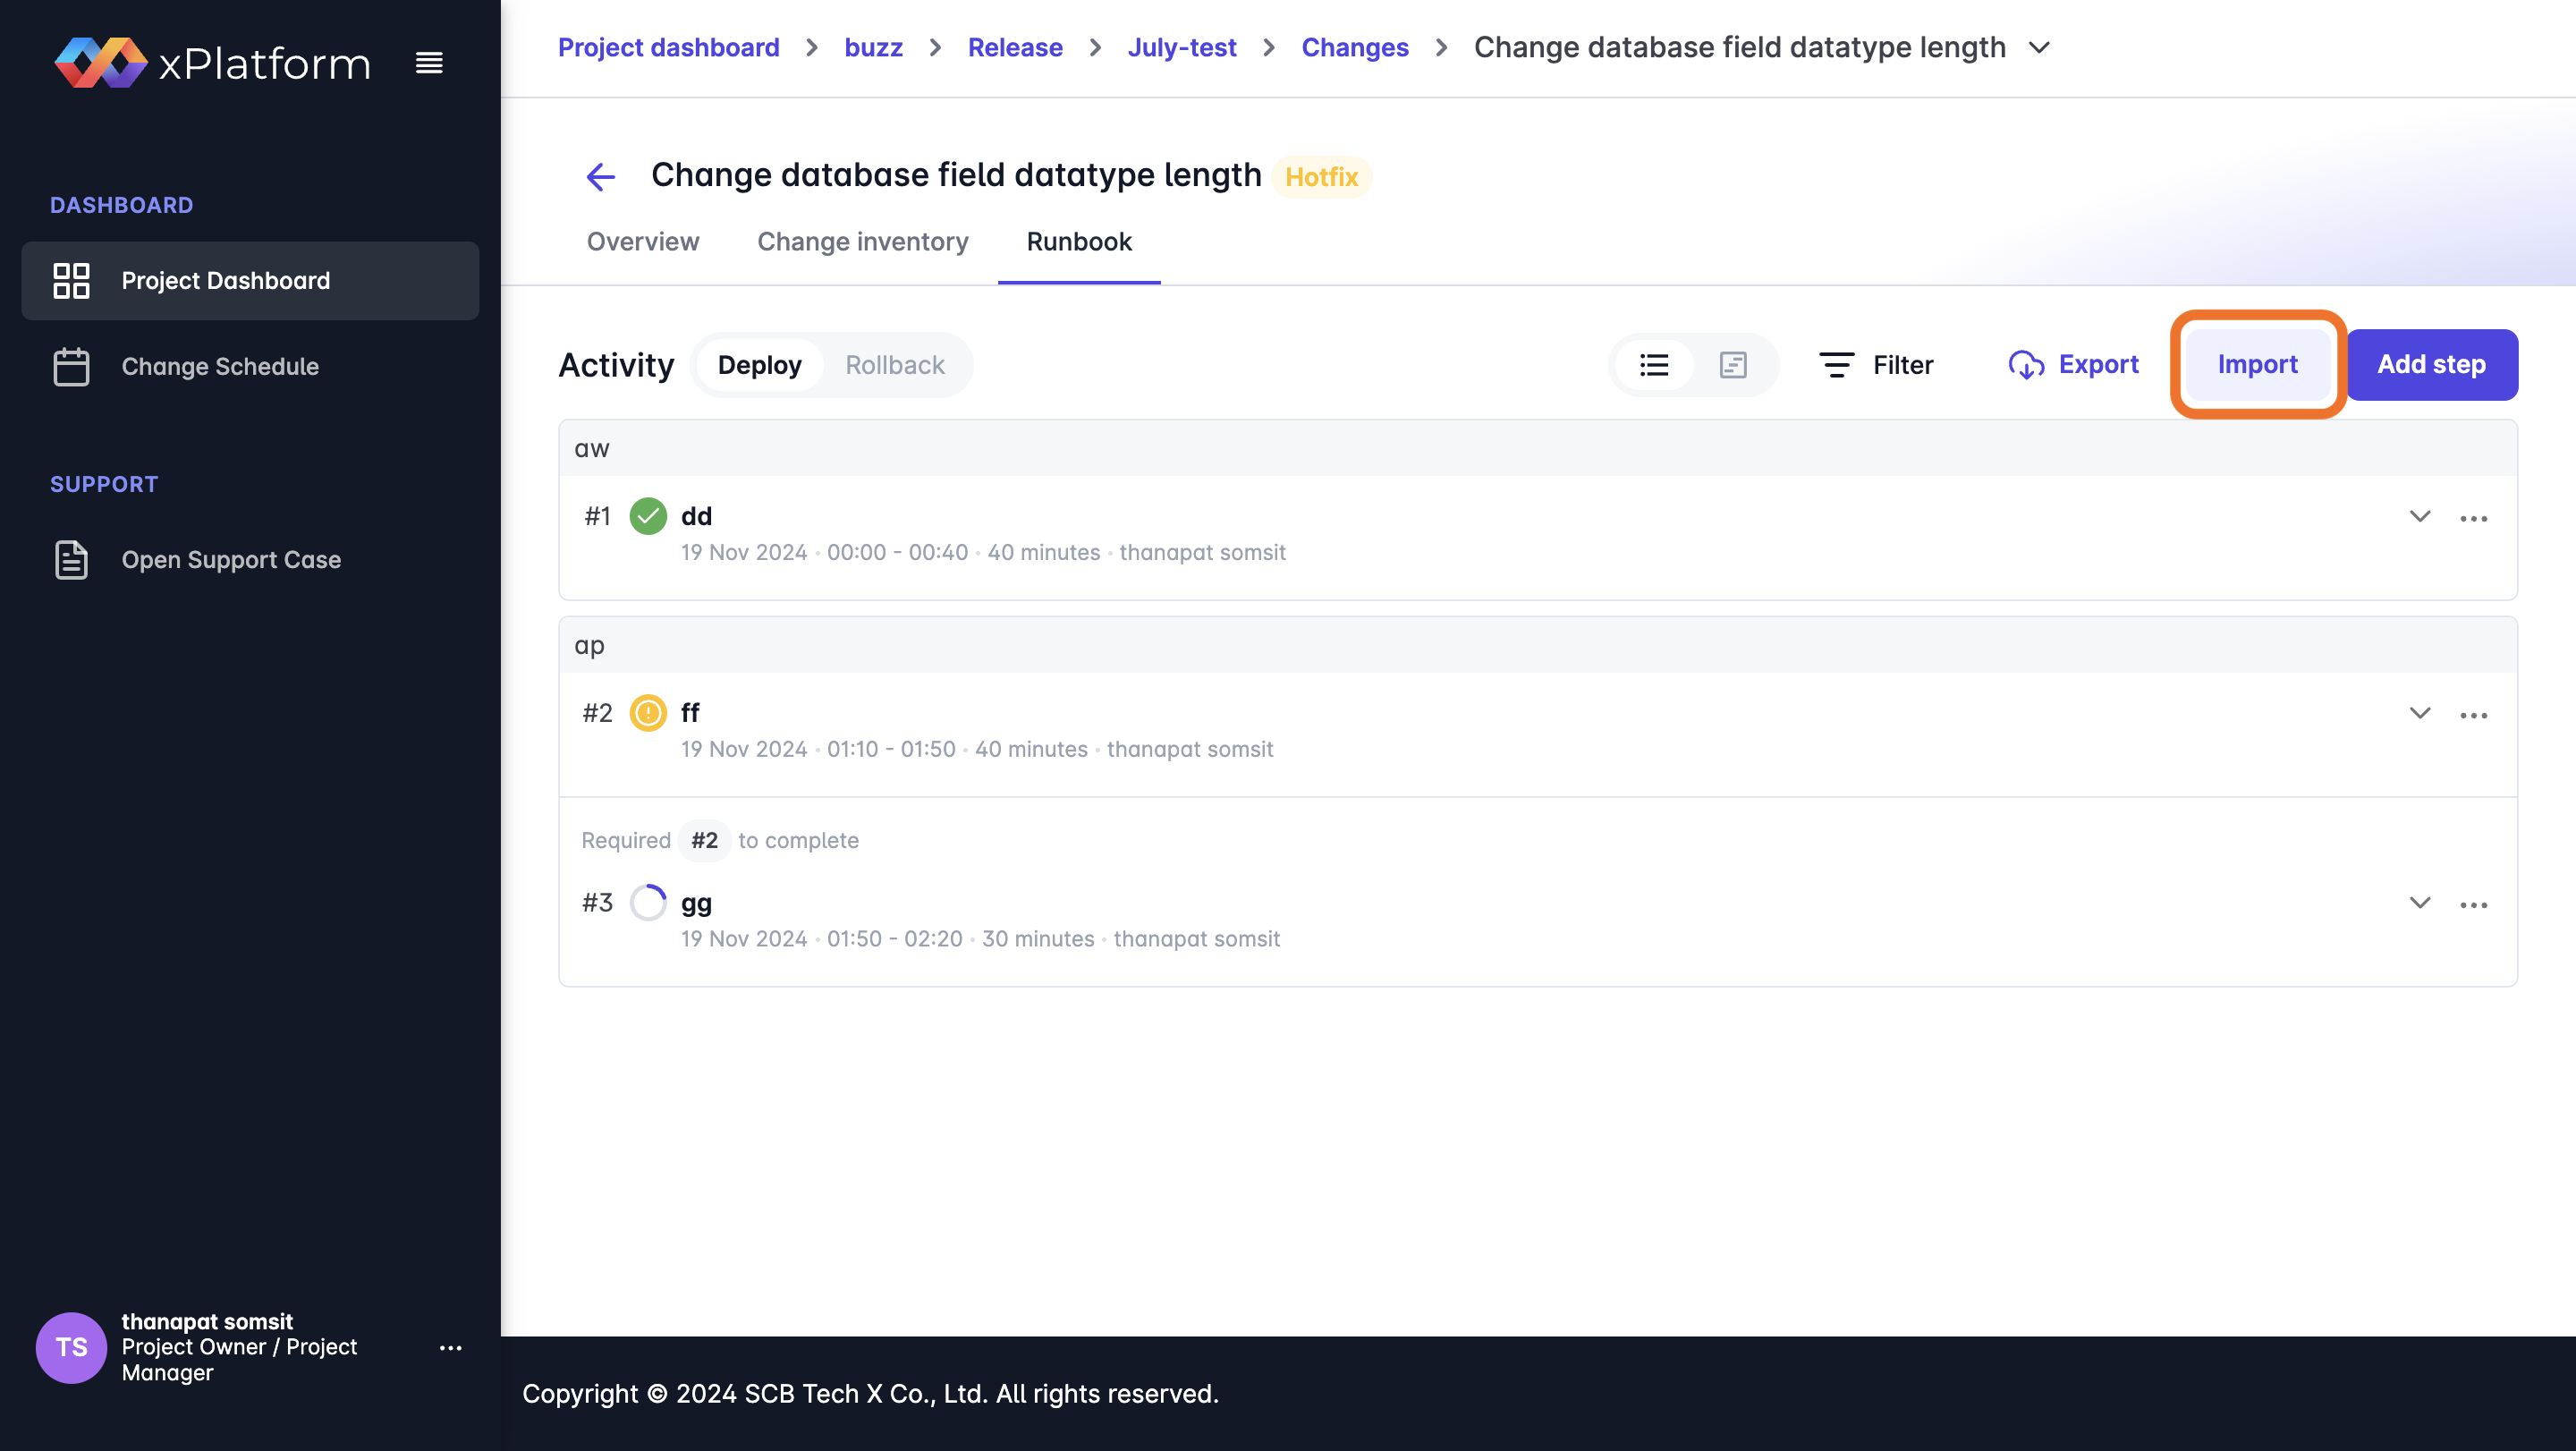
\includegraphics[width=\linewidth]{resources/pages/change-runbook/import-jira/22.png}

    \vspace{1in}

    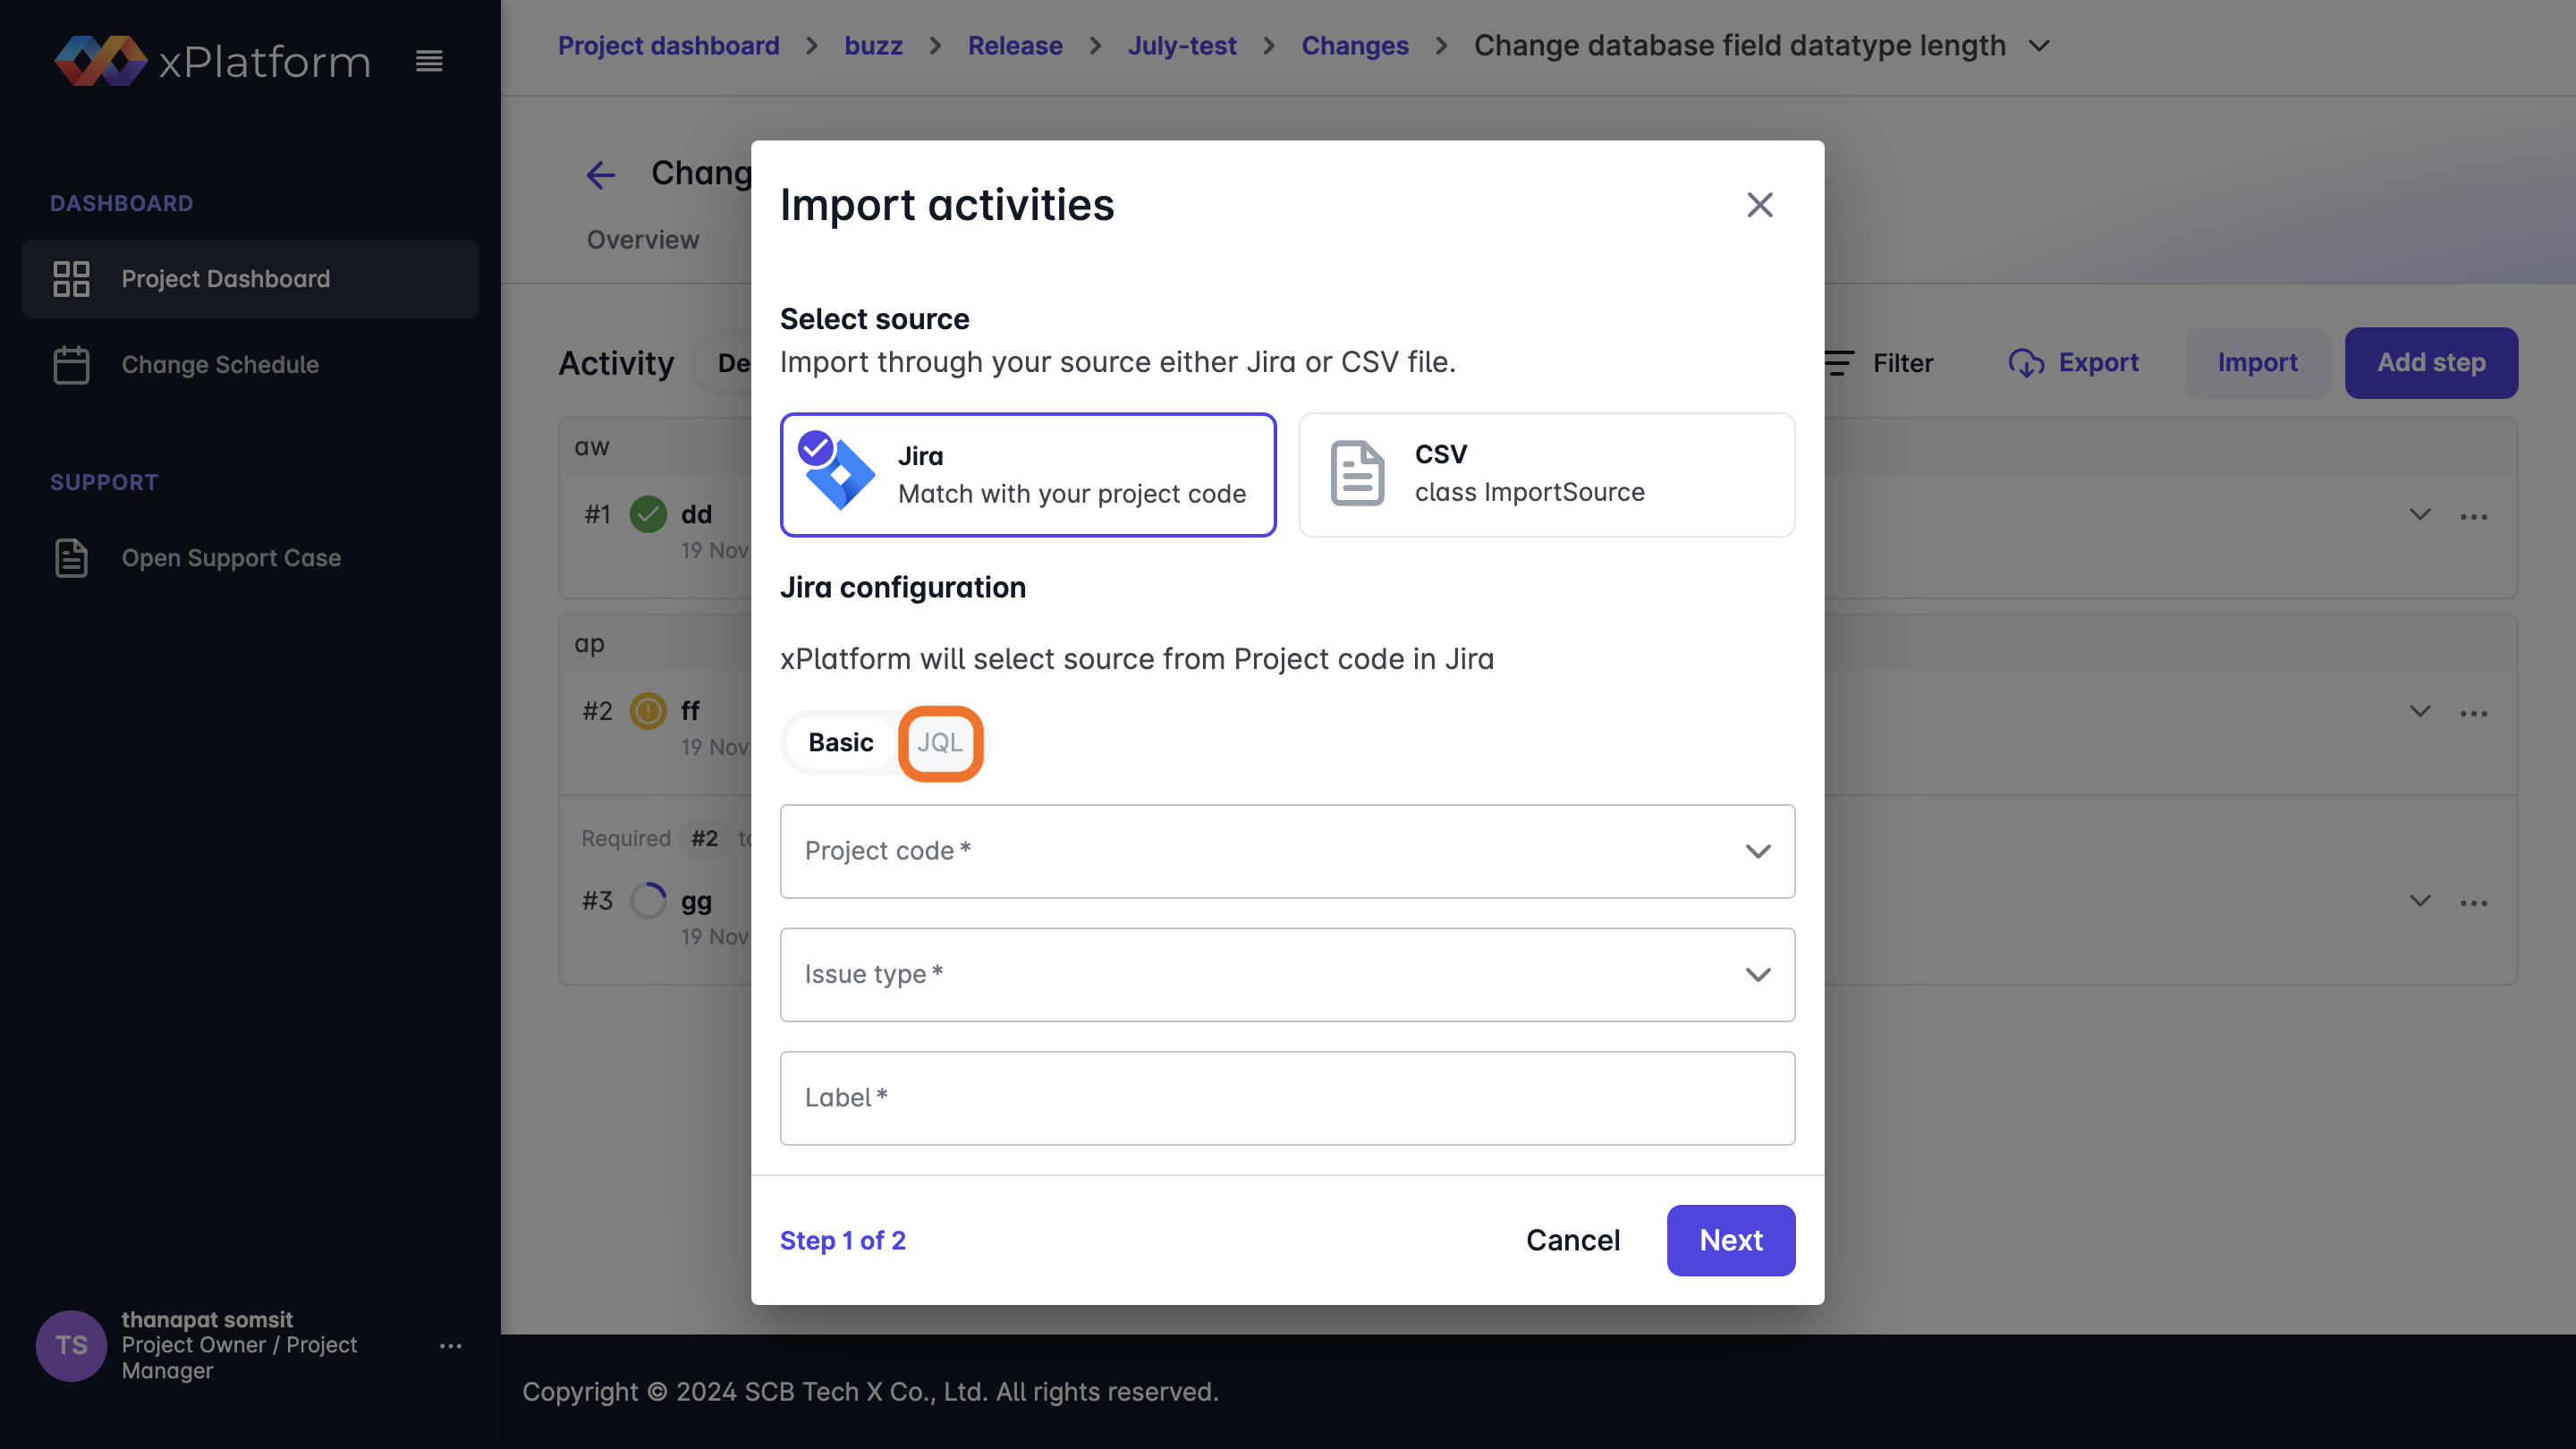
\includegraphics[width=\linewidth]{resources/pages/change-runbook/import-jira/23.png}
\end{center}
\begin{center}
    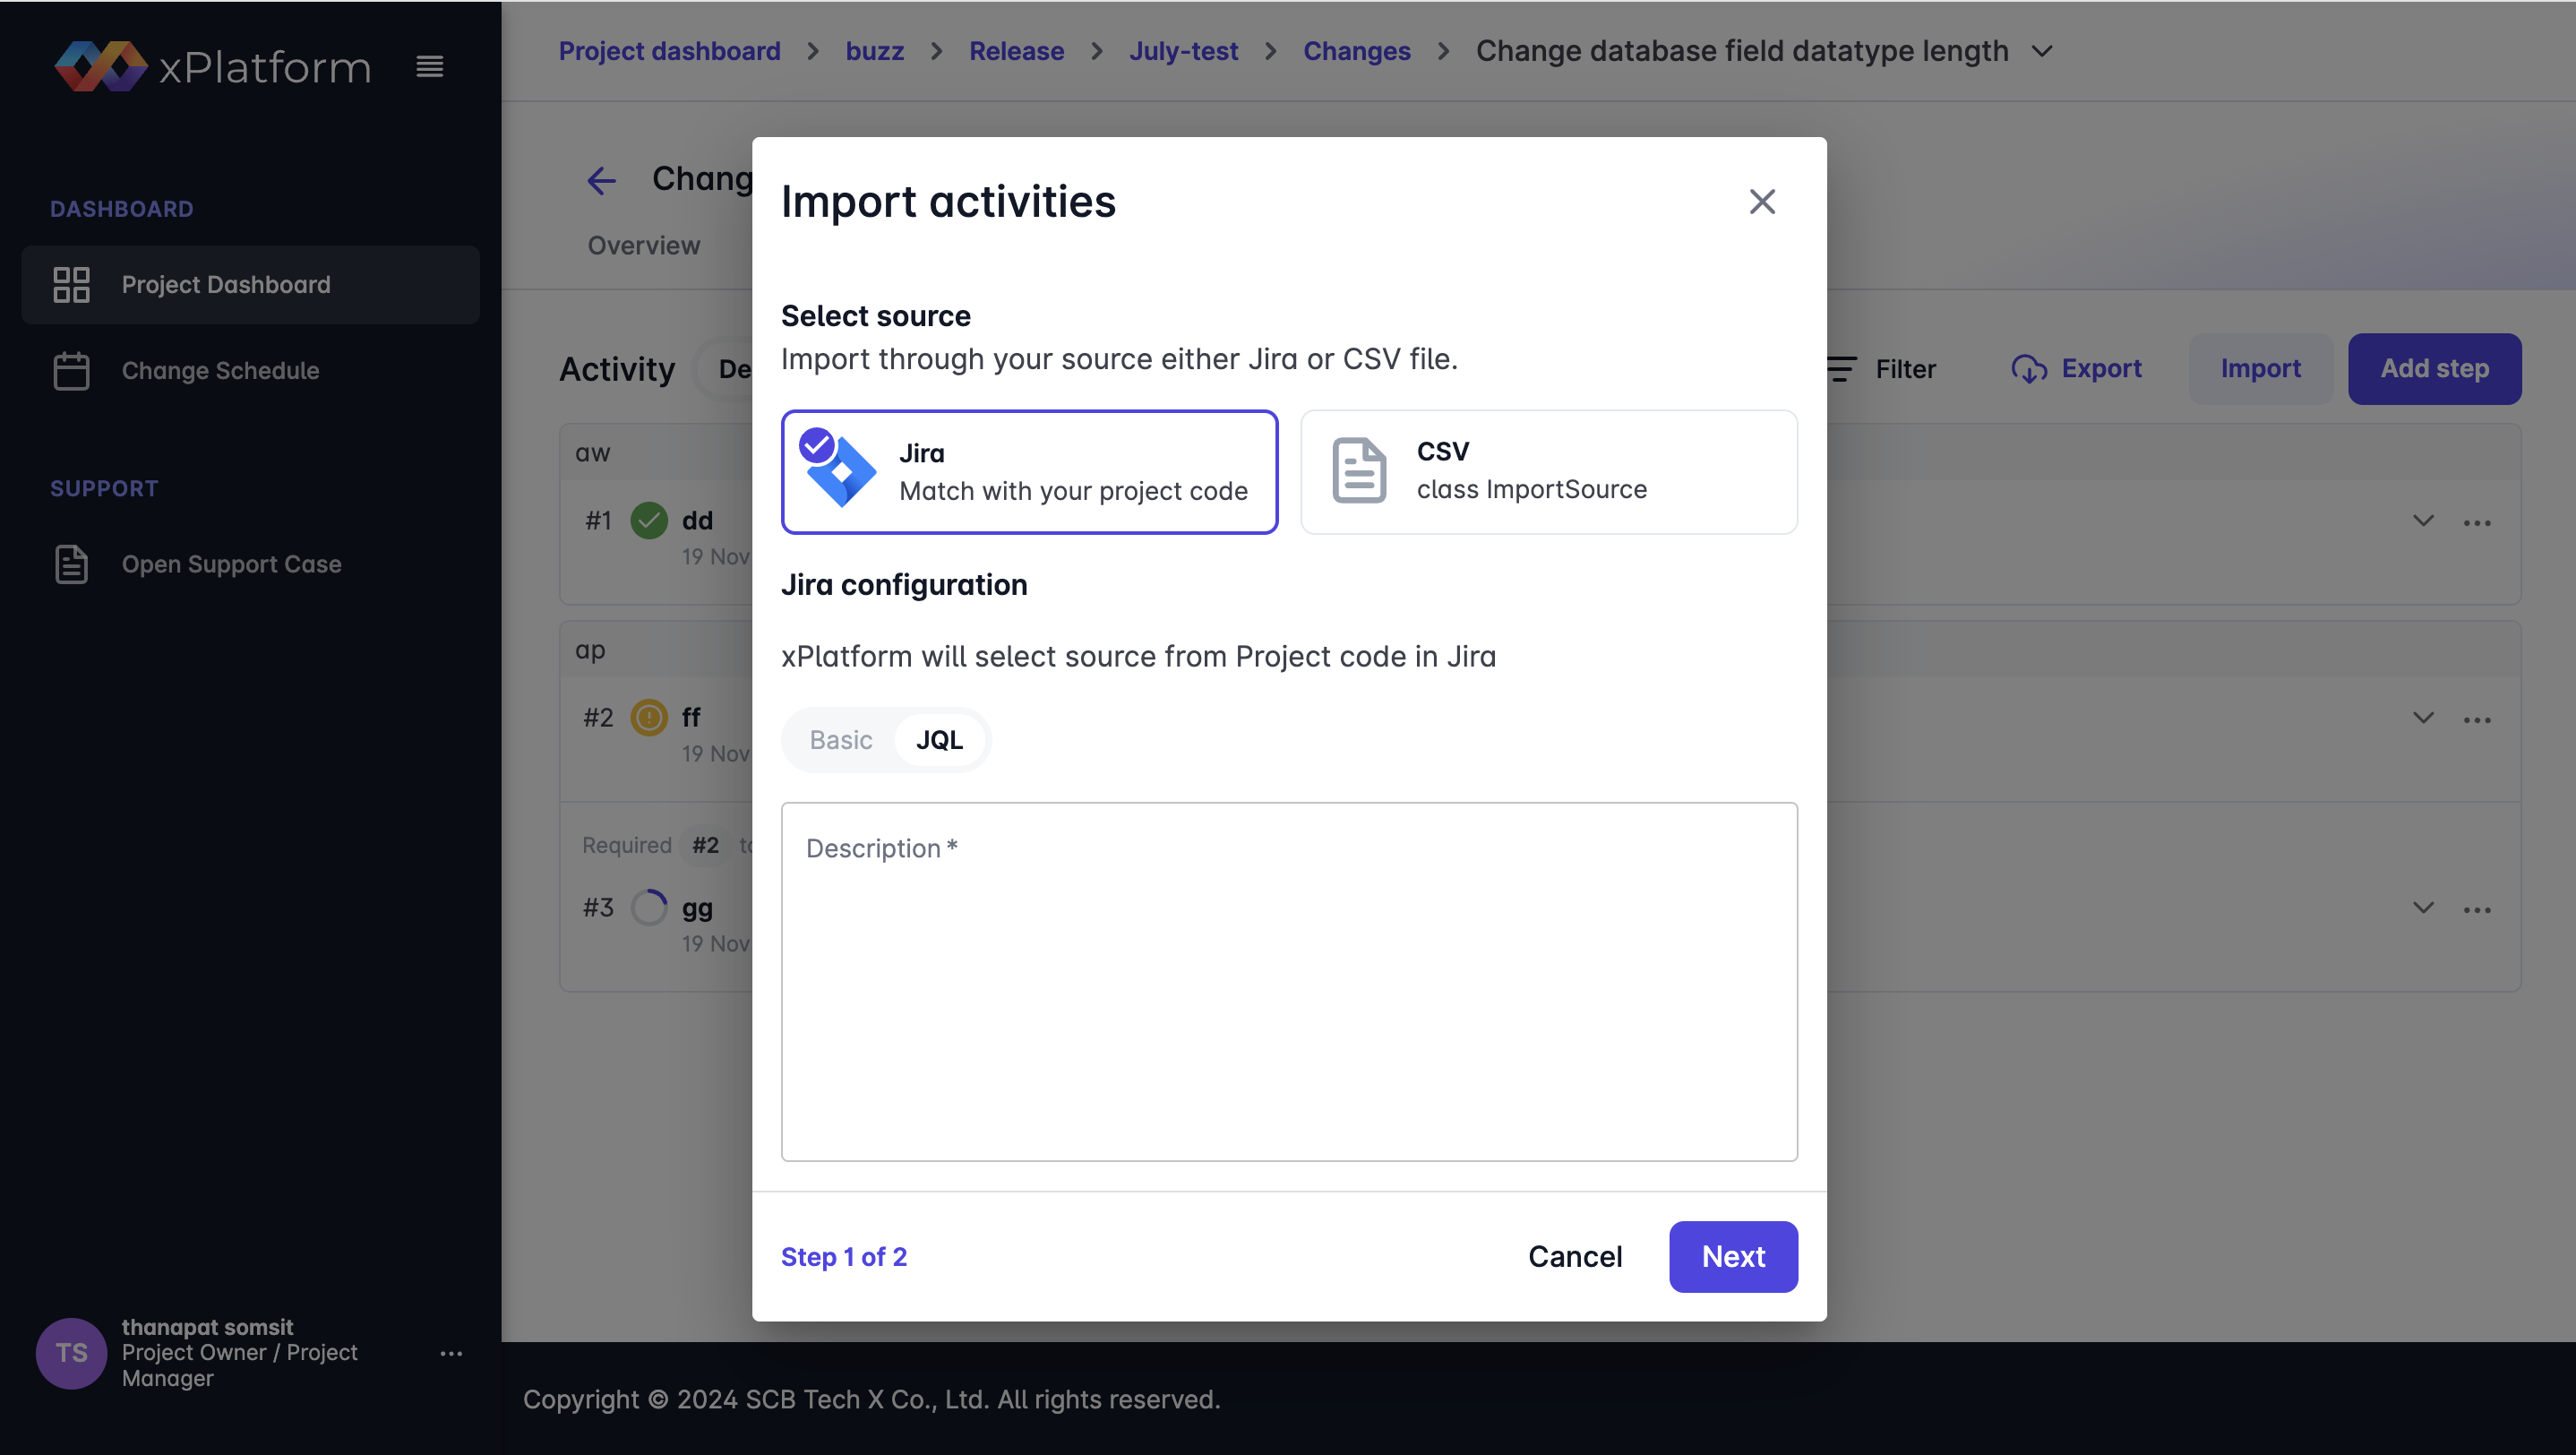
\includegraphics[width=\linewidth]{resources/pages/change-runbook/import-jira/24.png}

    \vspace{1in}

    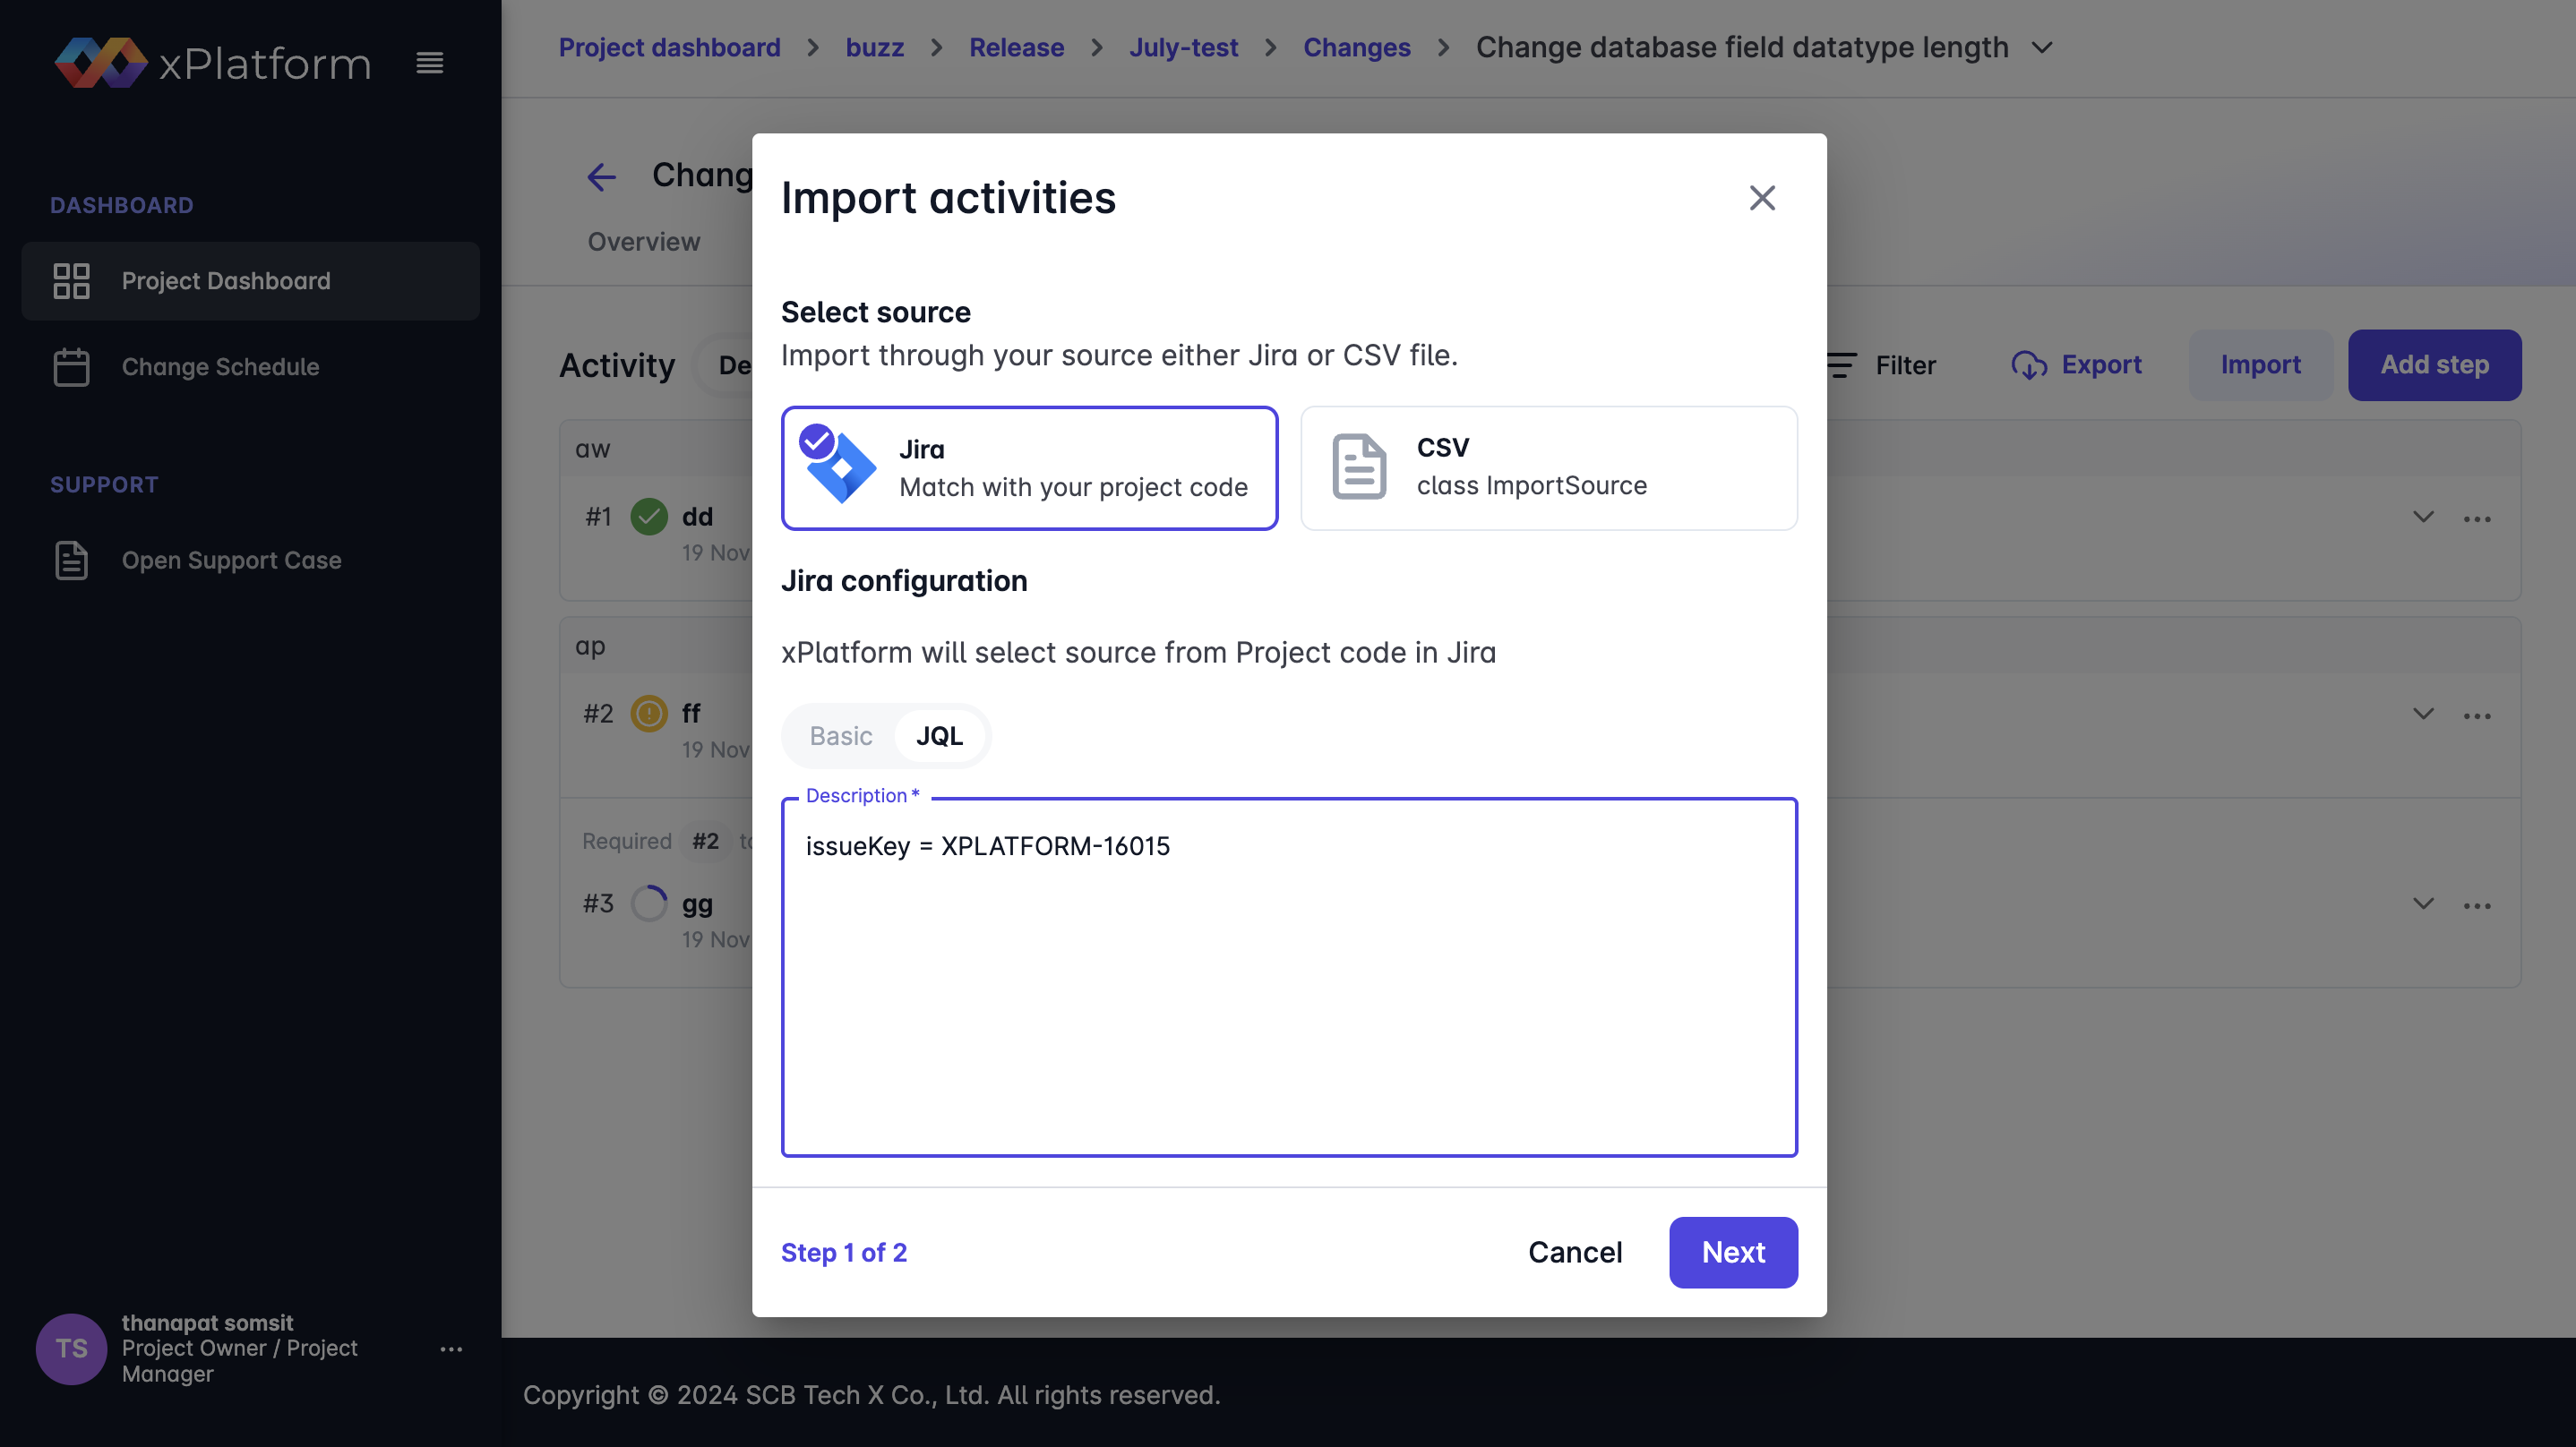
\includegraphics[width=\linewidth]{resources/pages/change-runbook/import-jira/25.png}
\end{center}
\begin{center}
    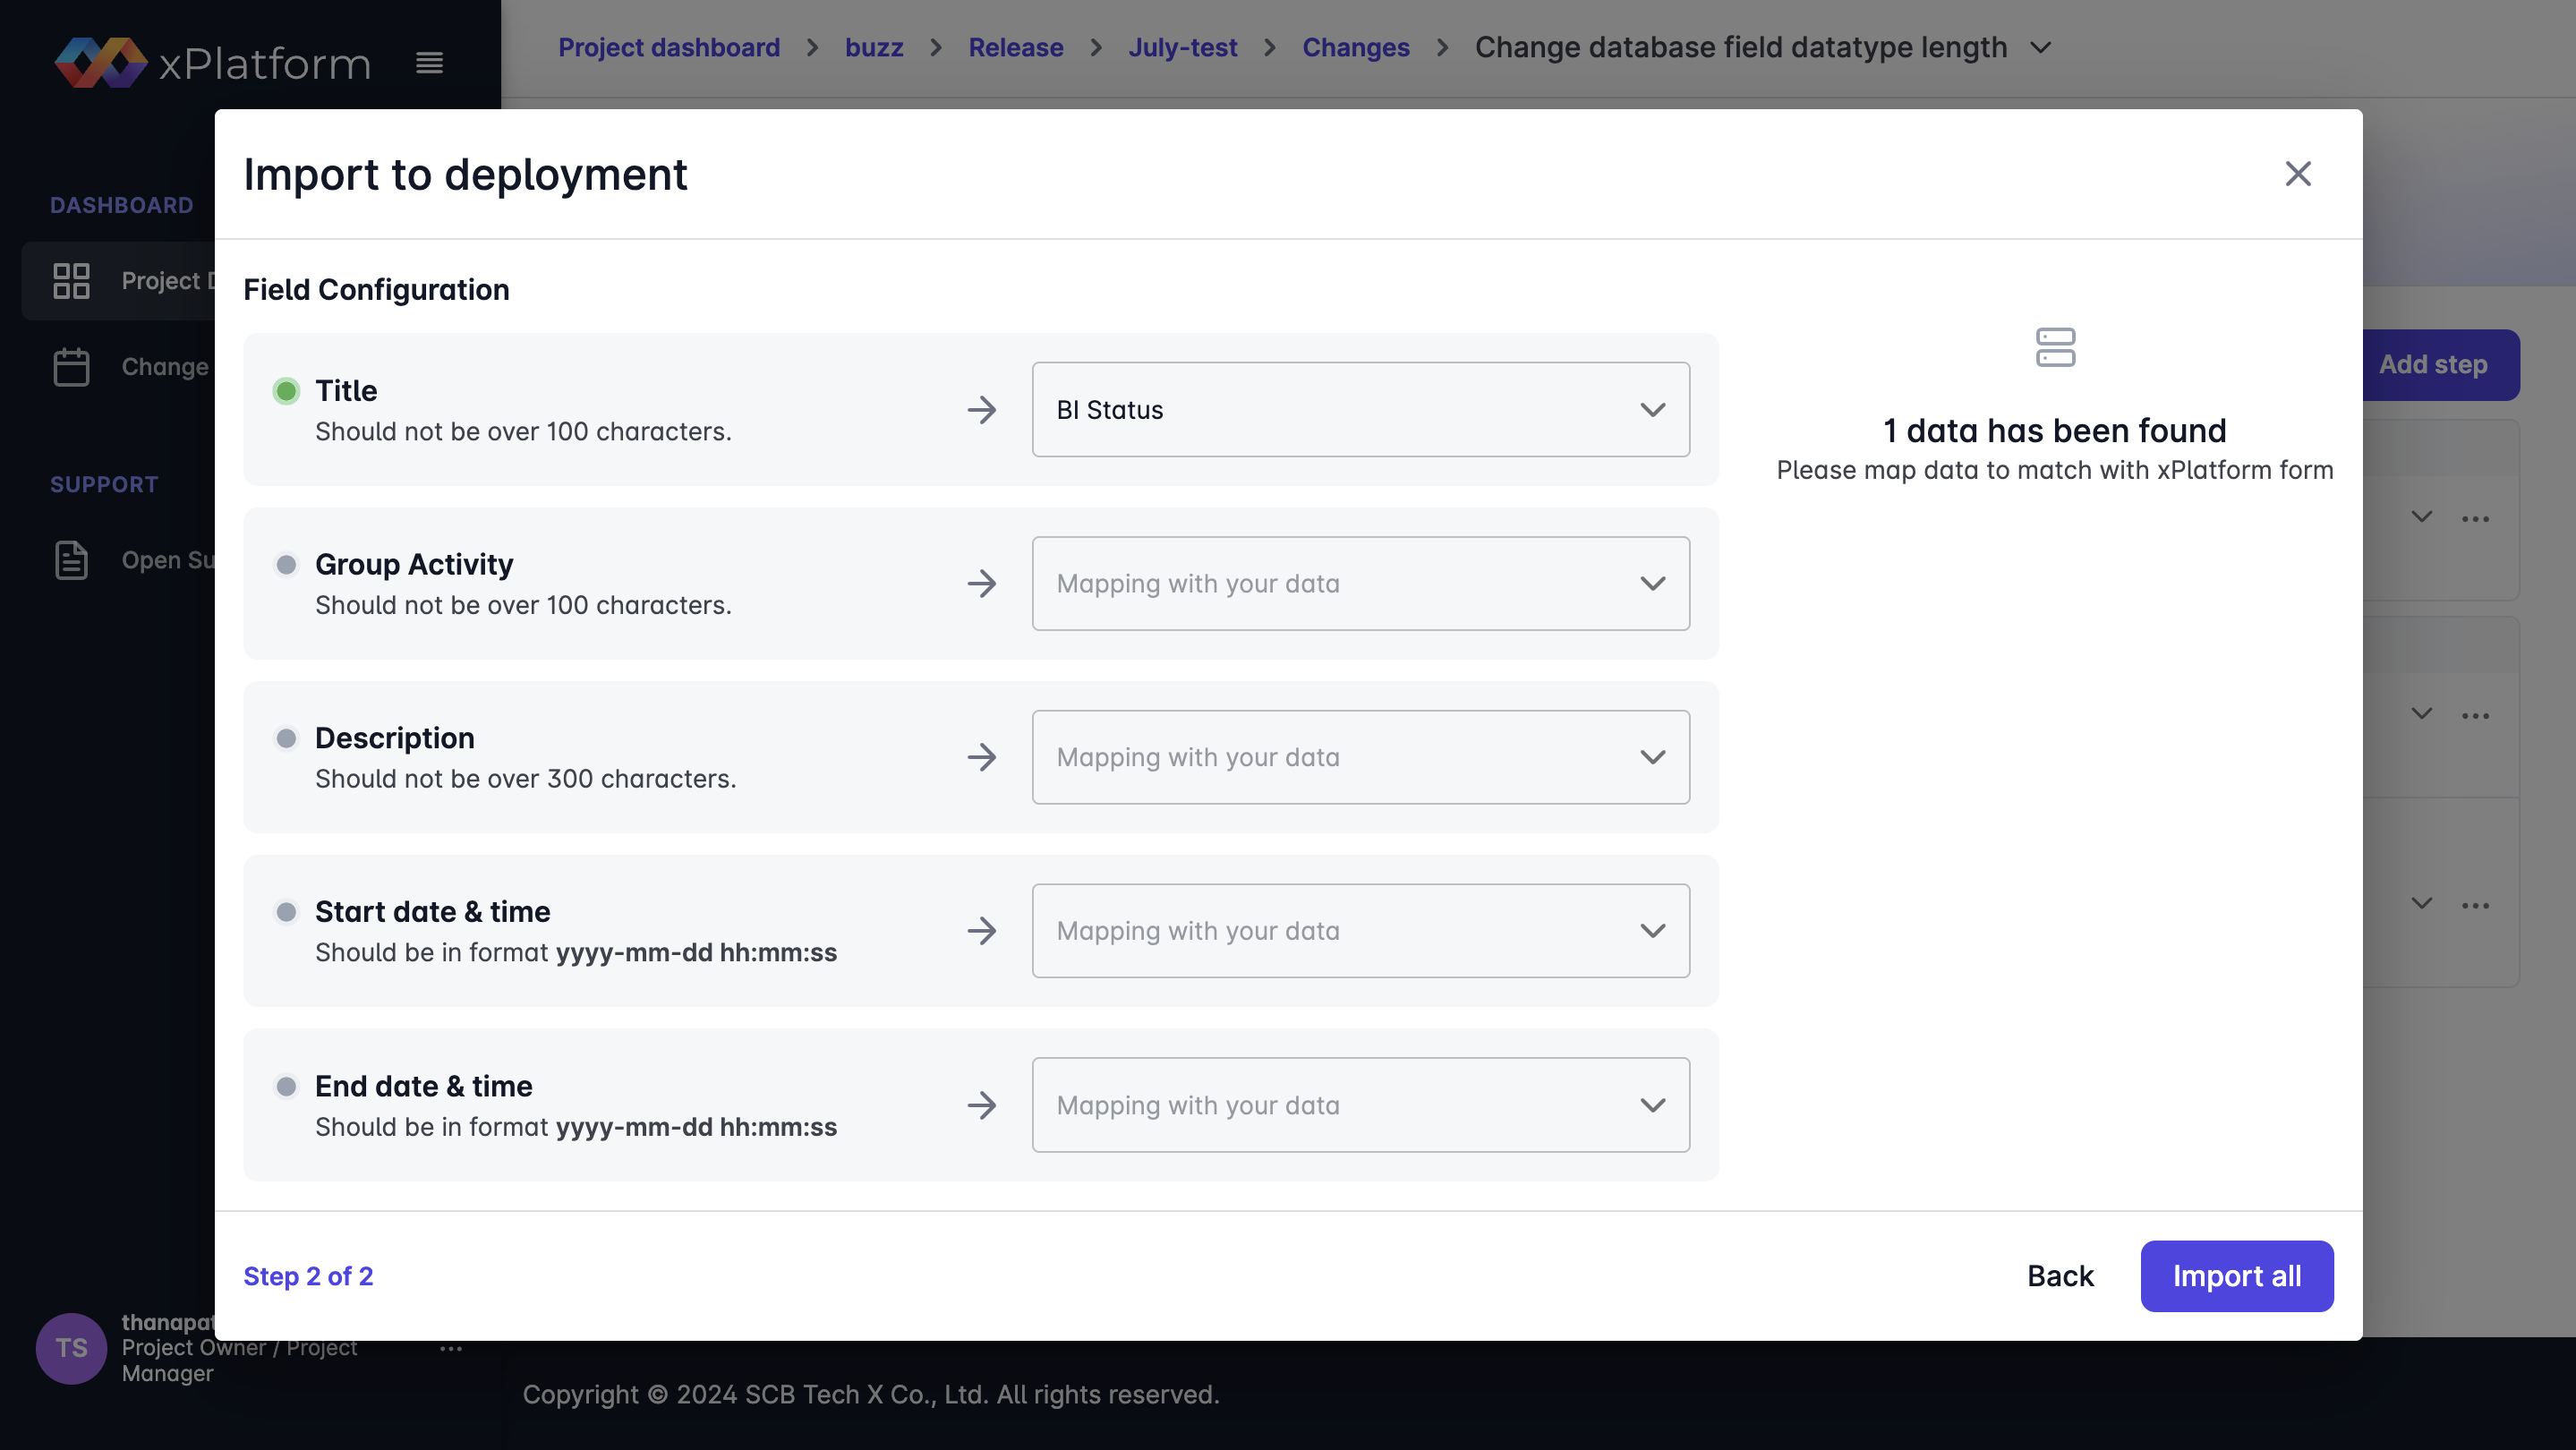
\includegraphics[width=\linewidth]{resources/pages/change-runbook/import-jira/26.png}

    \vspace{1in}

    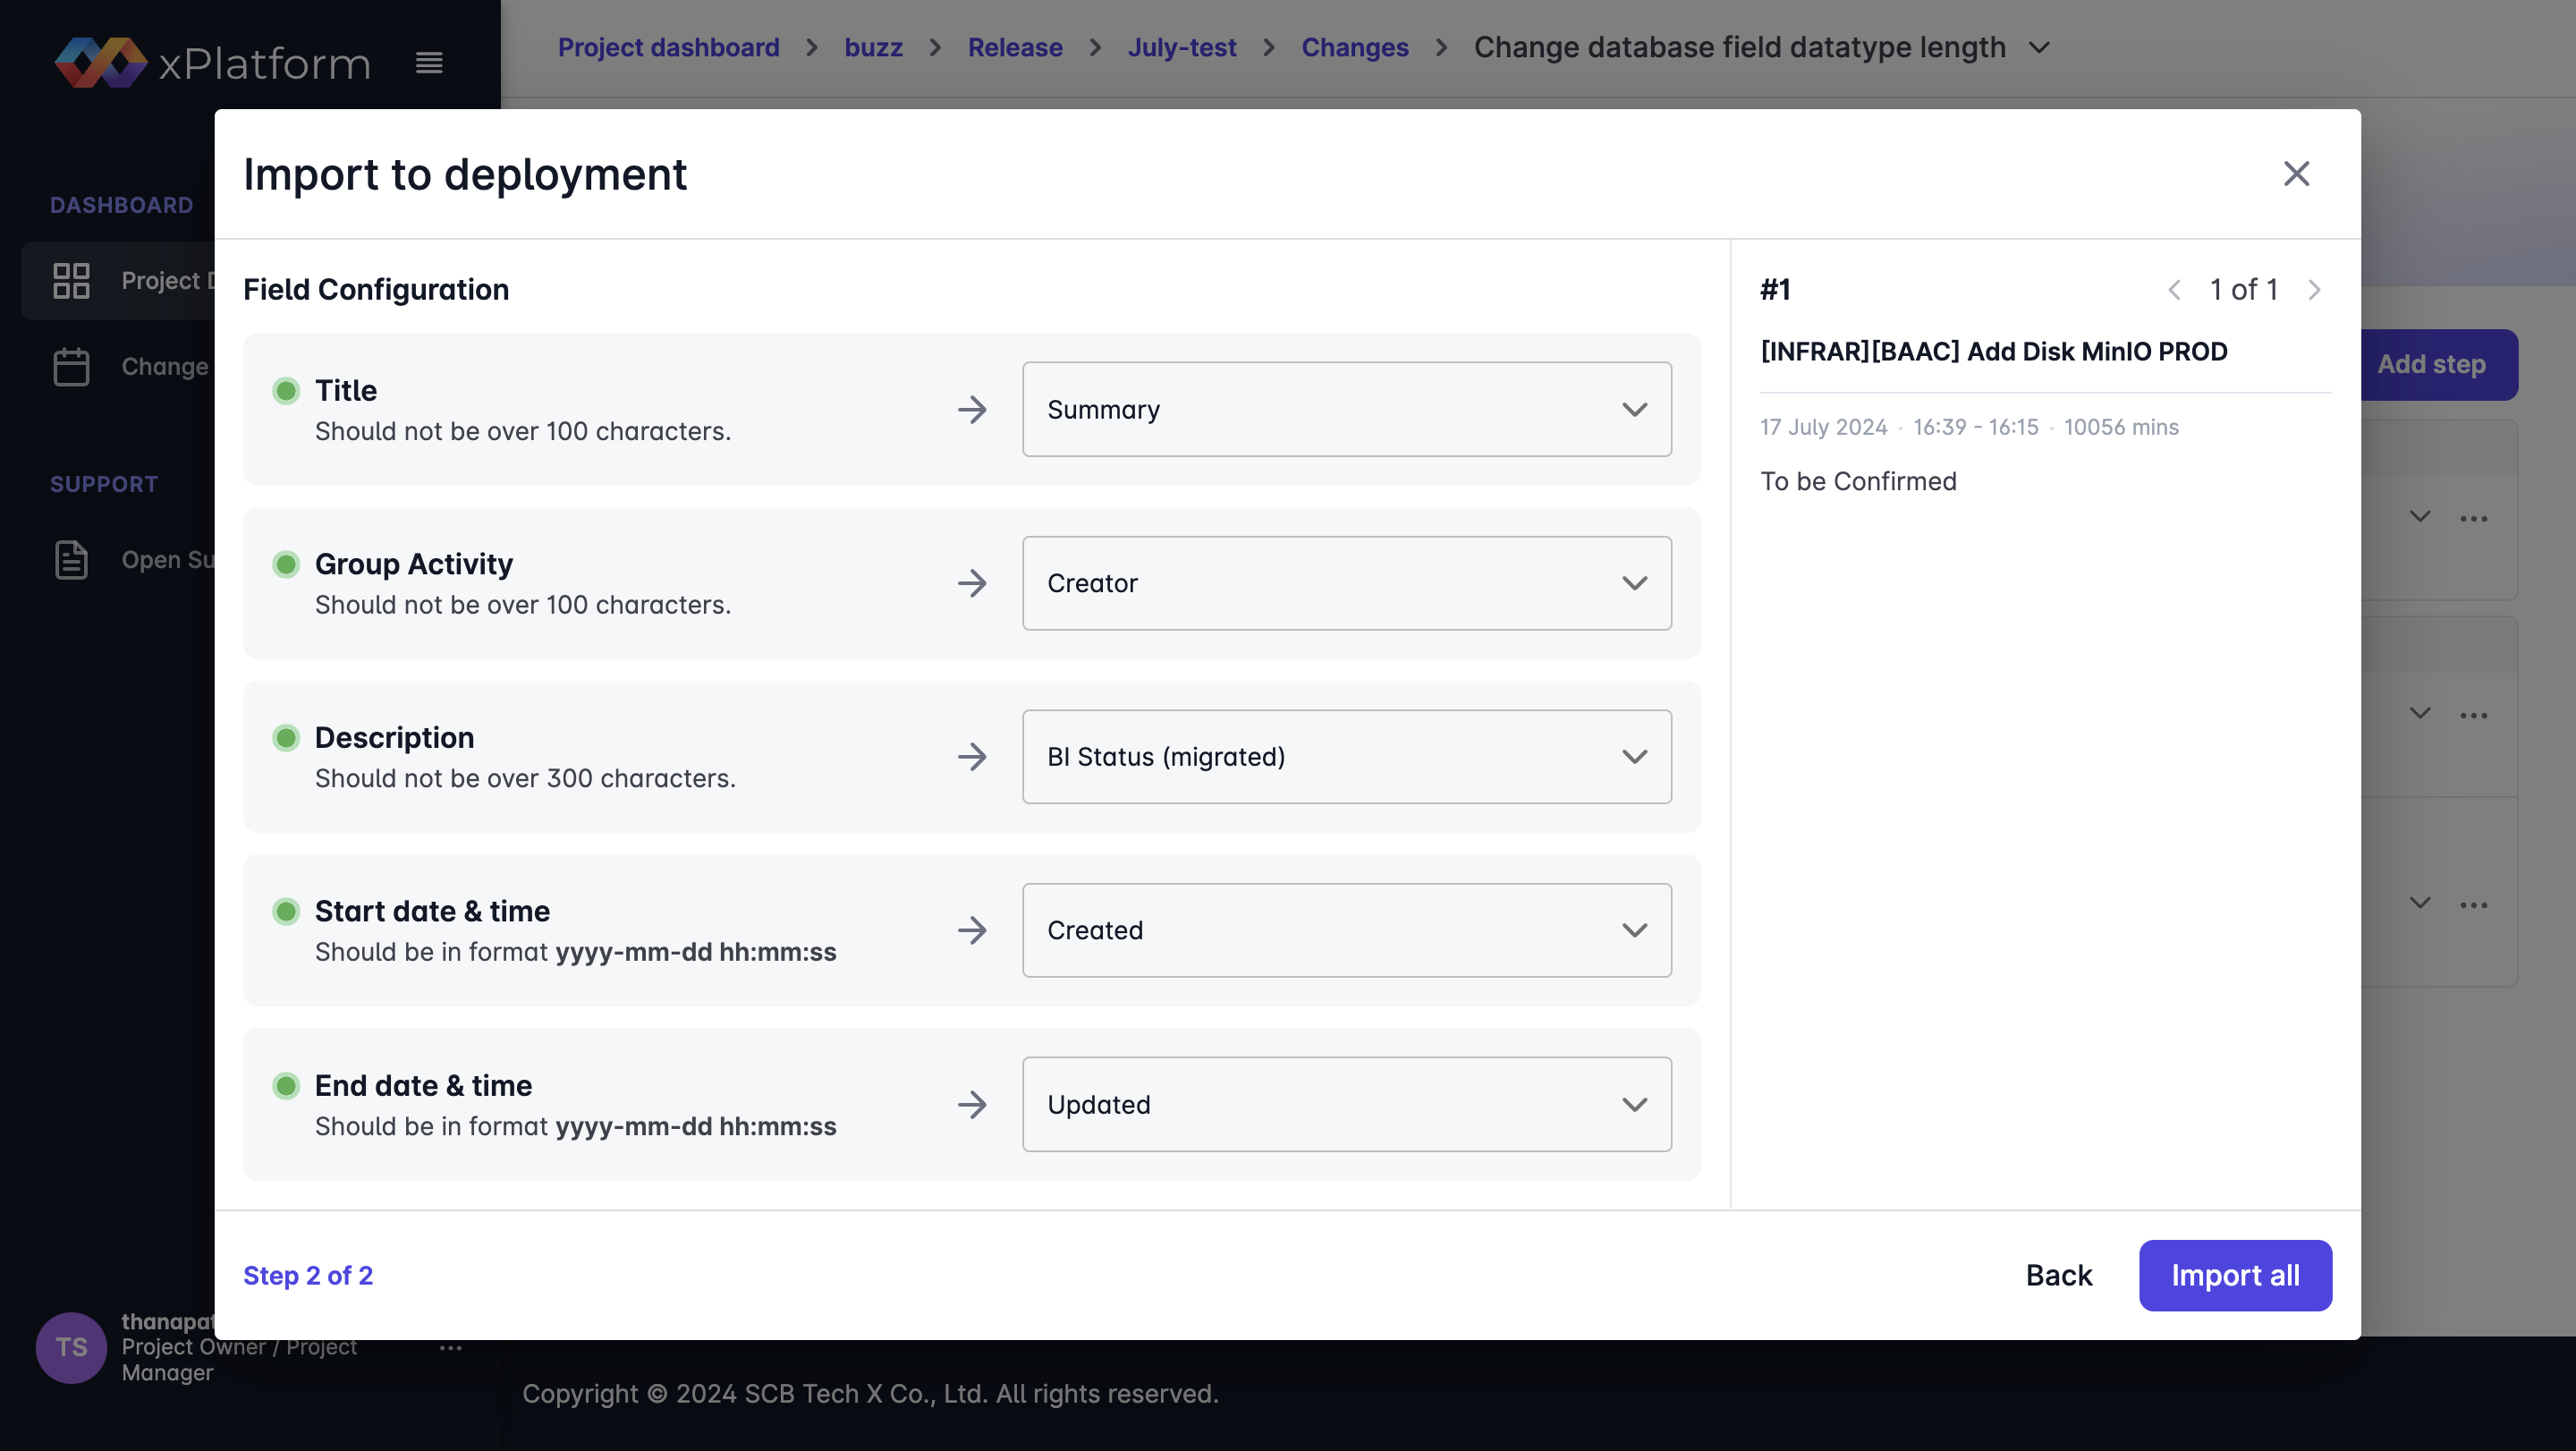
\includegraphics[width=\linewidth]{resources/pages/change-runbook/import-jira/27.png}
\end{center}

\begin{figure}[H]
    \begin{center}
        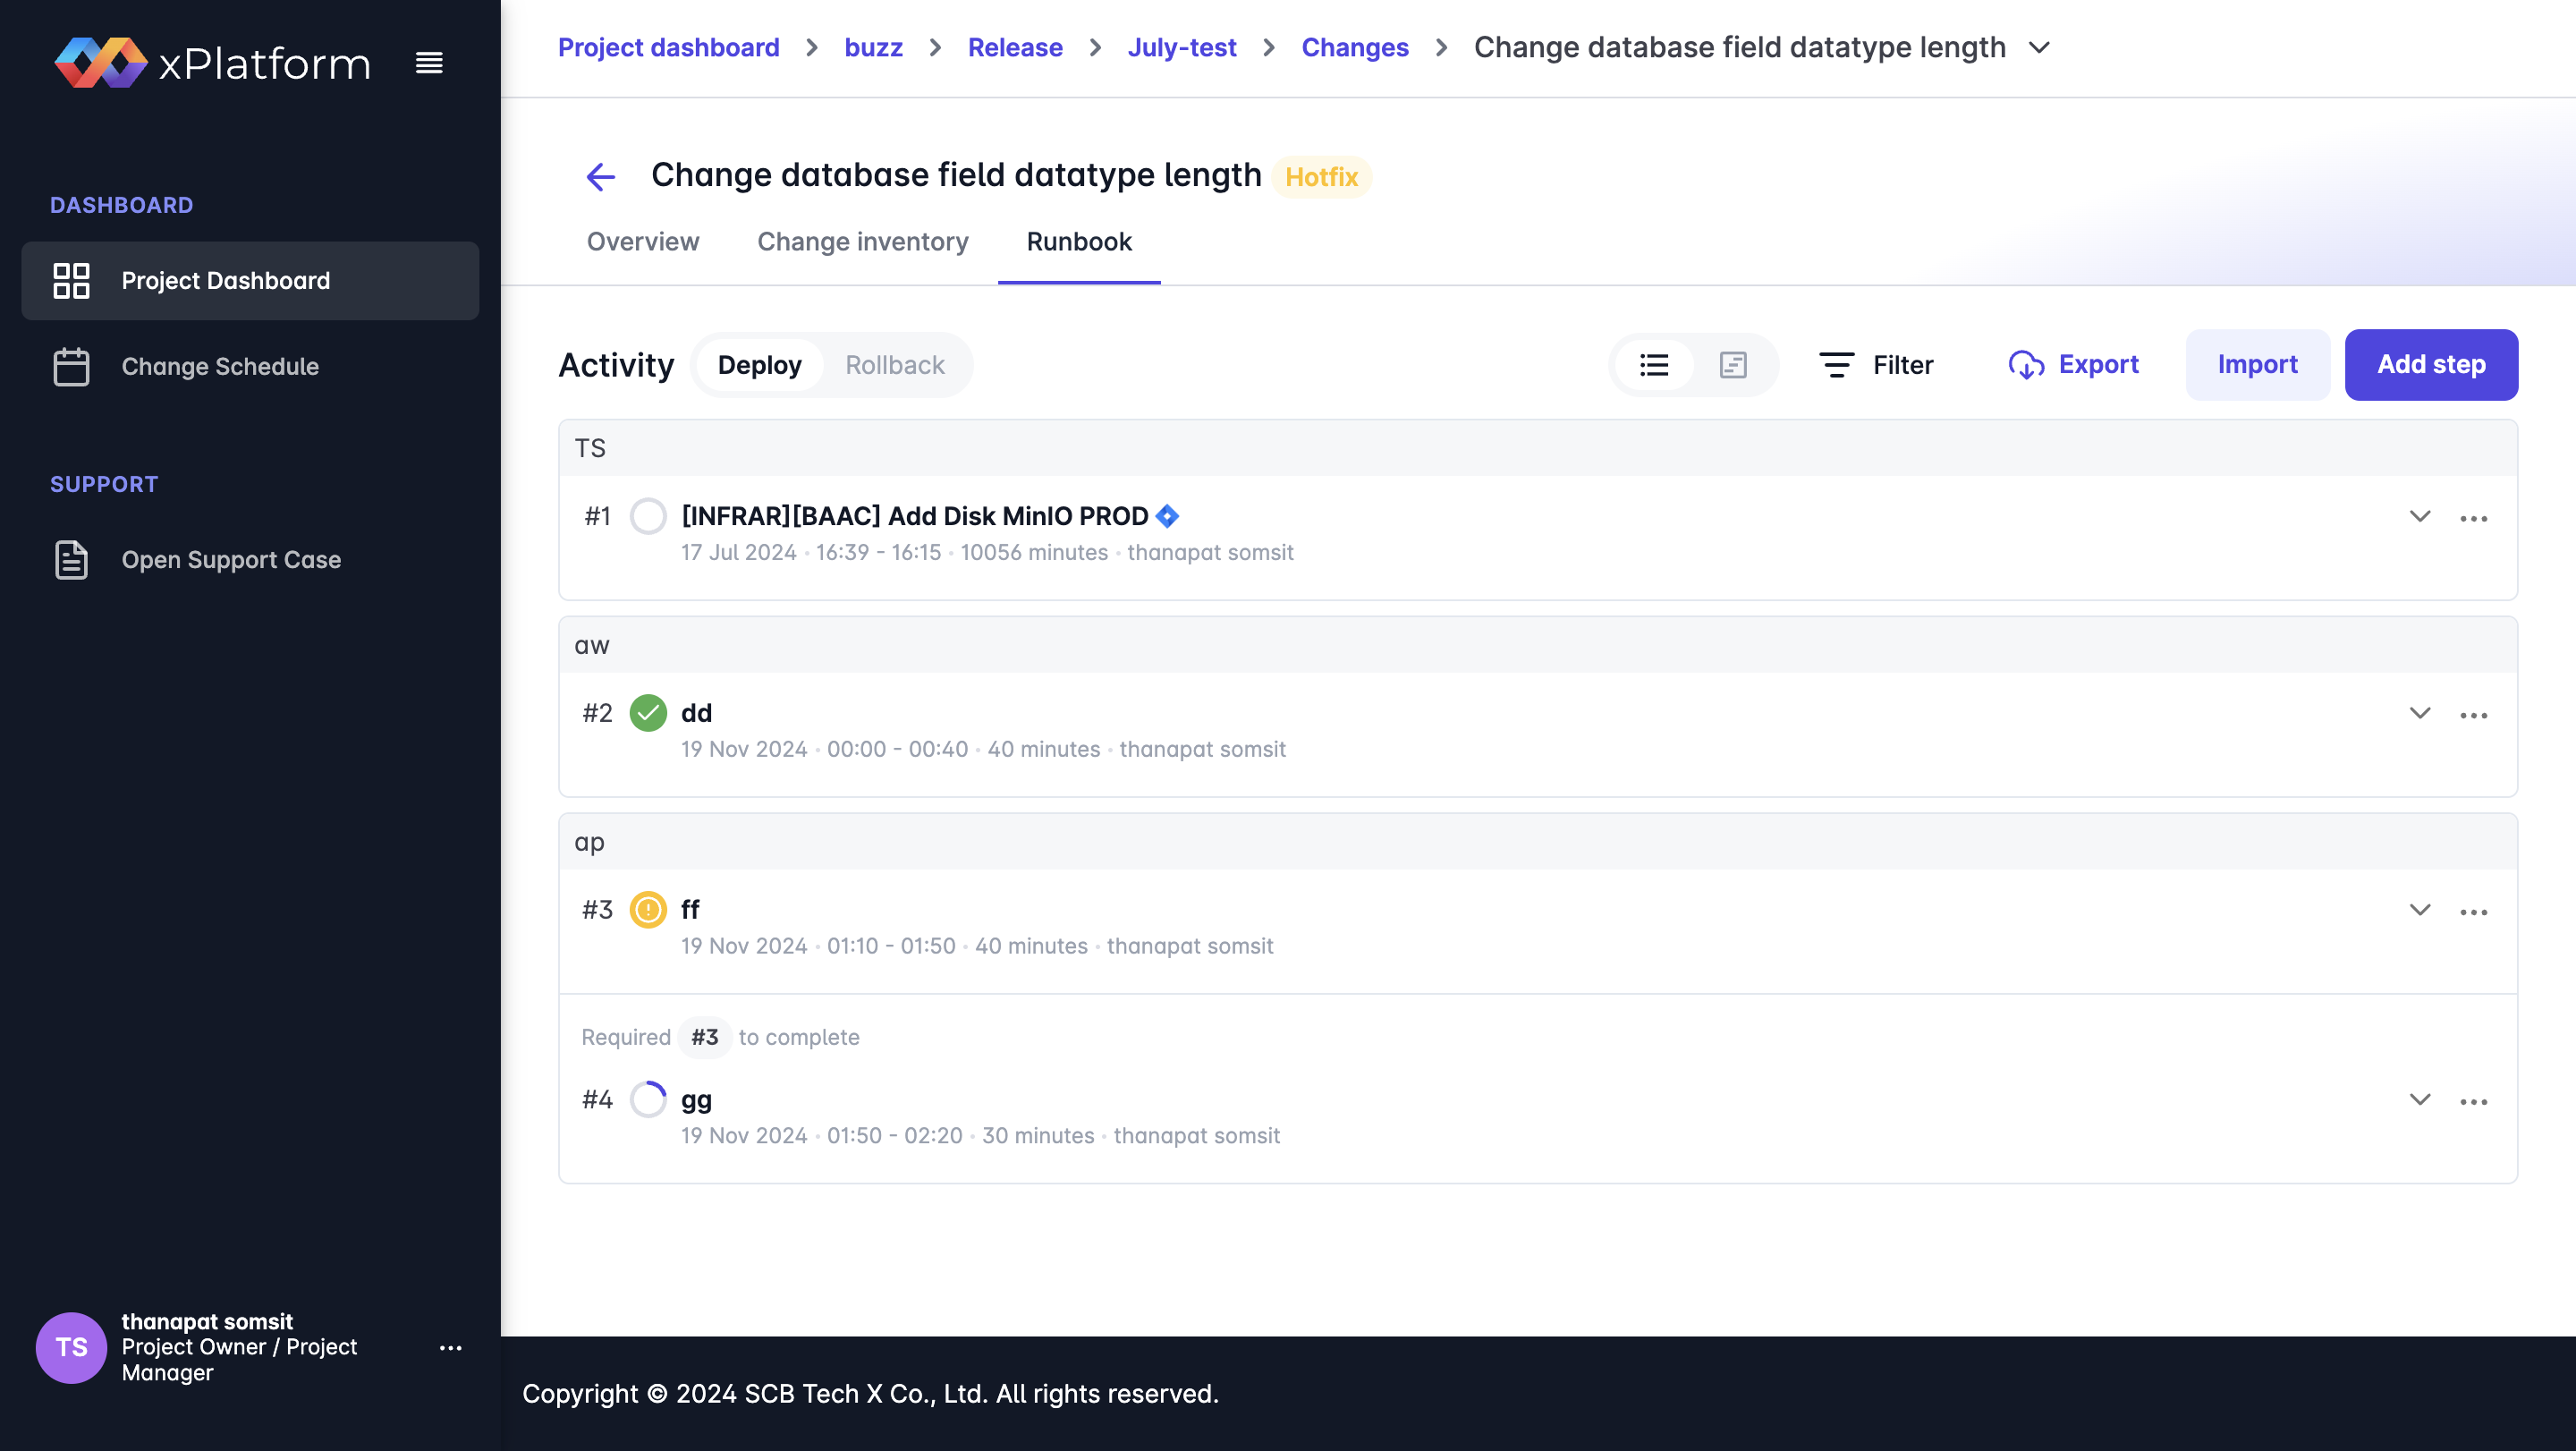
\includegraphics[width=\linewidth]{resources/pages/change-runbook/import-jira/28.png}
    \end{center}
    \caption[การดึงข้อมูลจาก Jira]{การดึงข้อมูลจาก Jira}
  \label{fig:import-jira}
\end{figure}

\newpage
\subsection{การดึงข้อมูลจาก CSV}
\begin{center}
    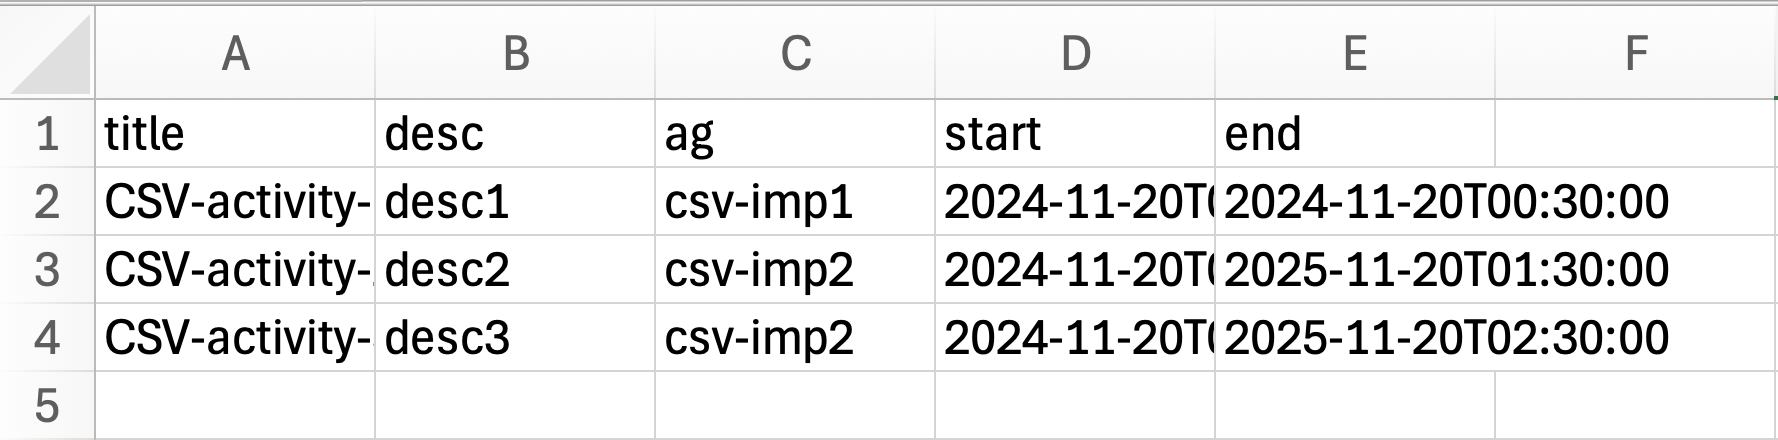
\includegraphics[width=\linewidth]{resources/pages/change-runbook/import-csv/29.png}

    \vspace{1in}

    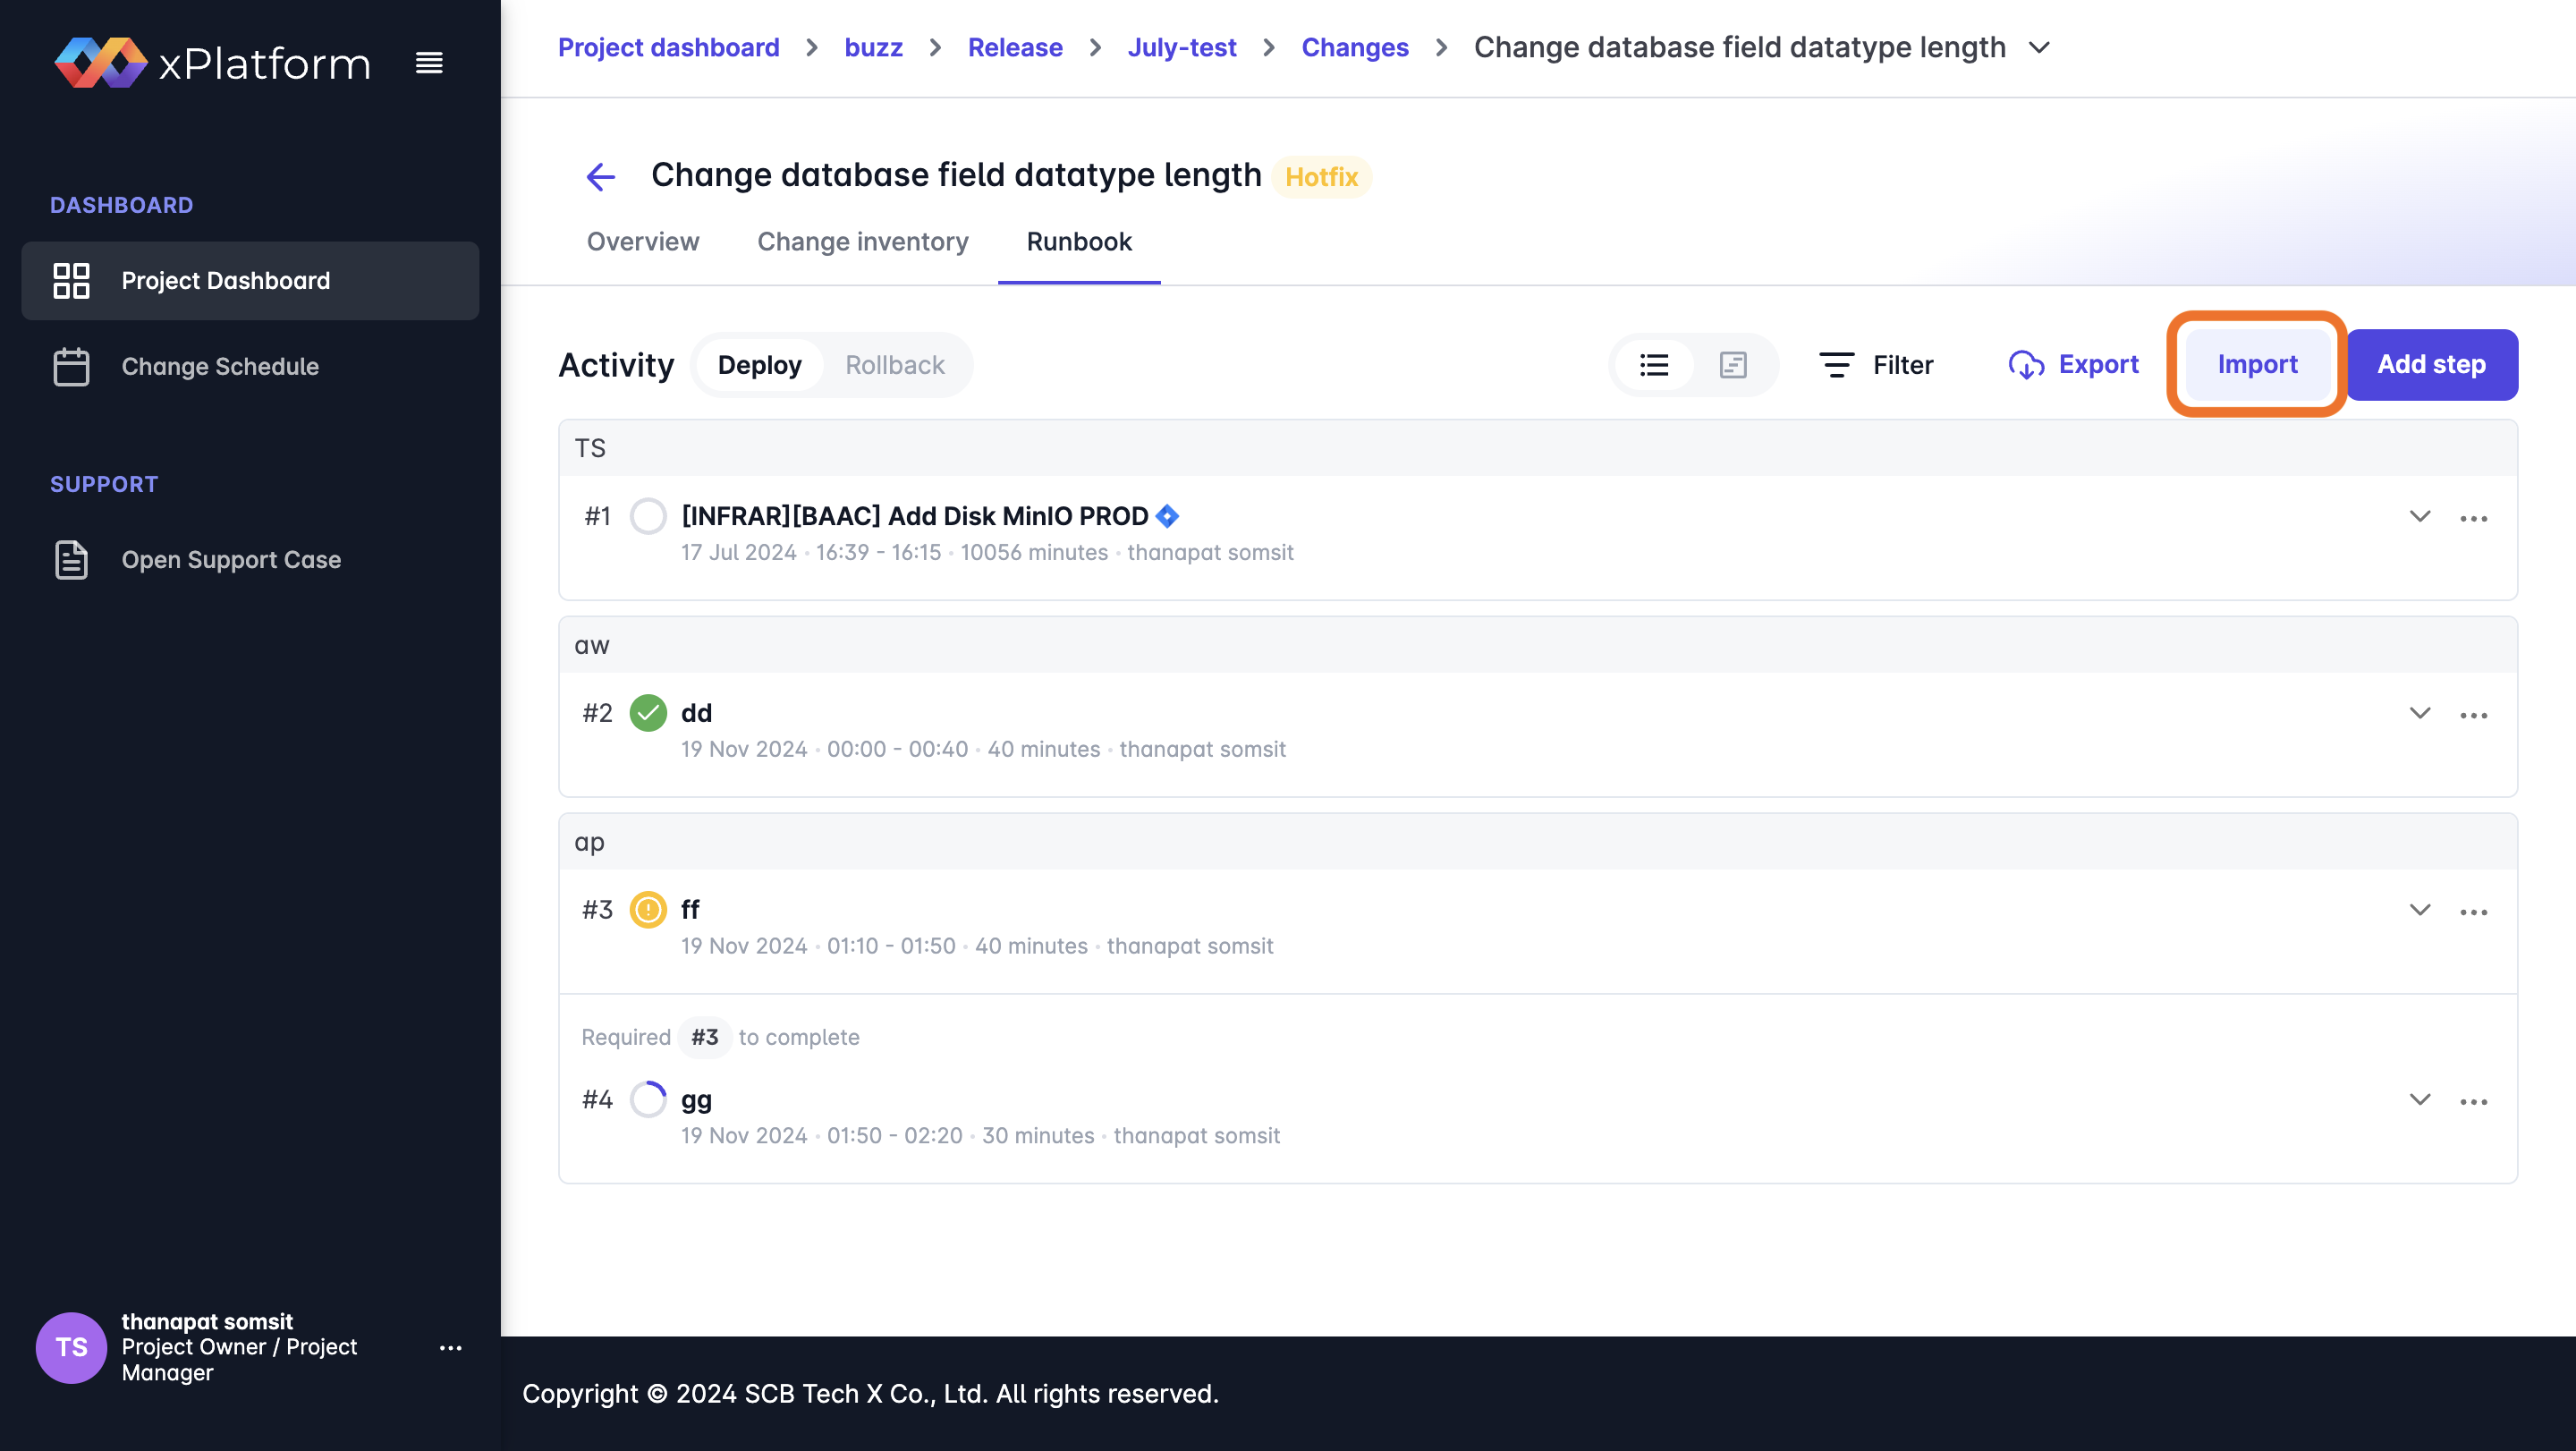
\includegraphics[width=\linewidth]{resources/pages/change-runbook/import-csv/30.png}
\end{center}
\begin{center}
    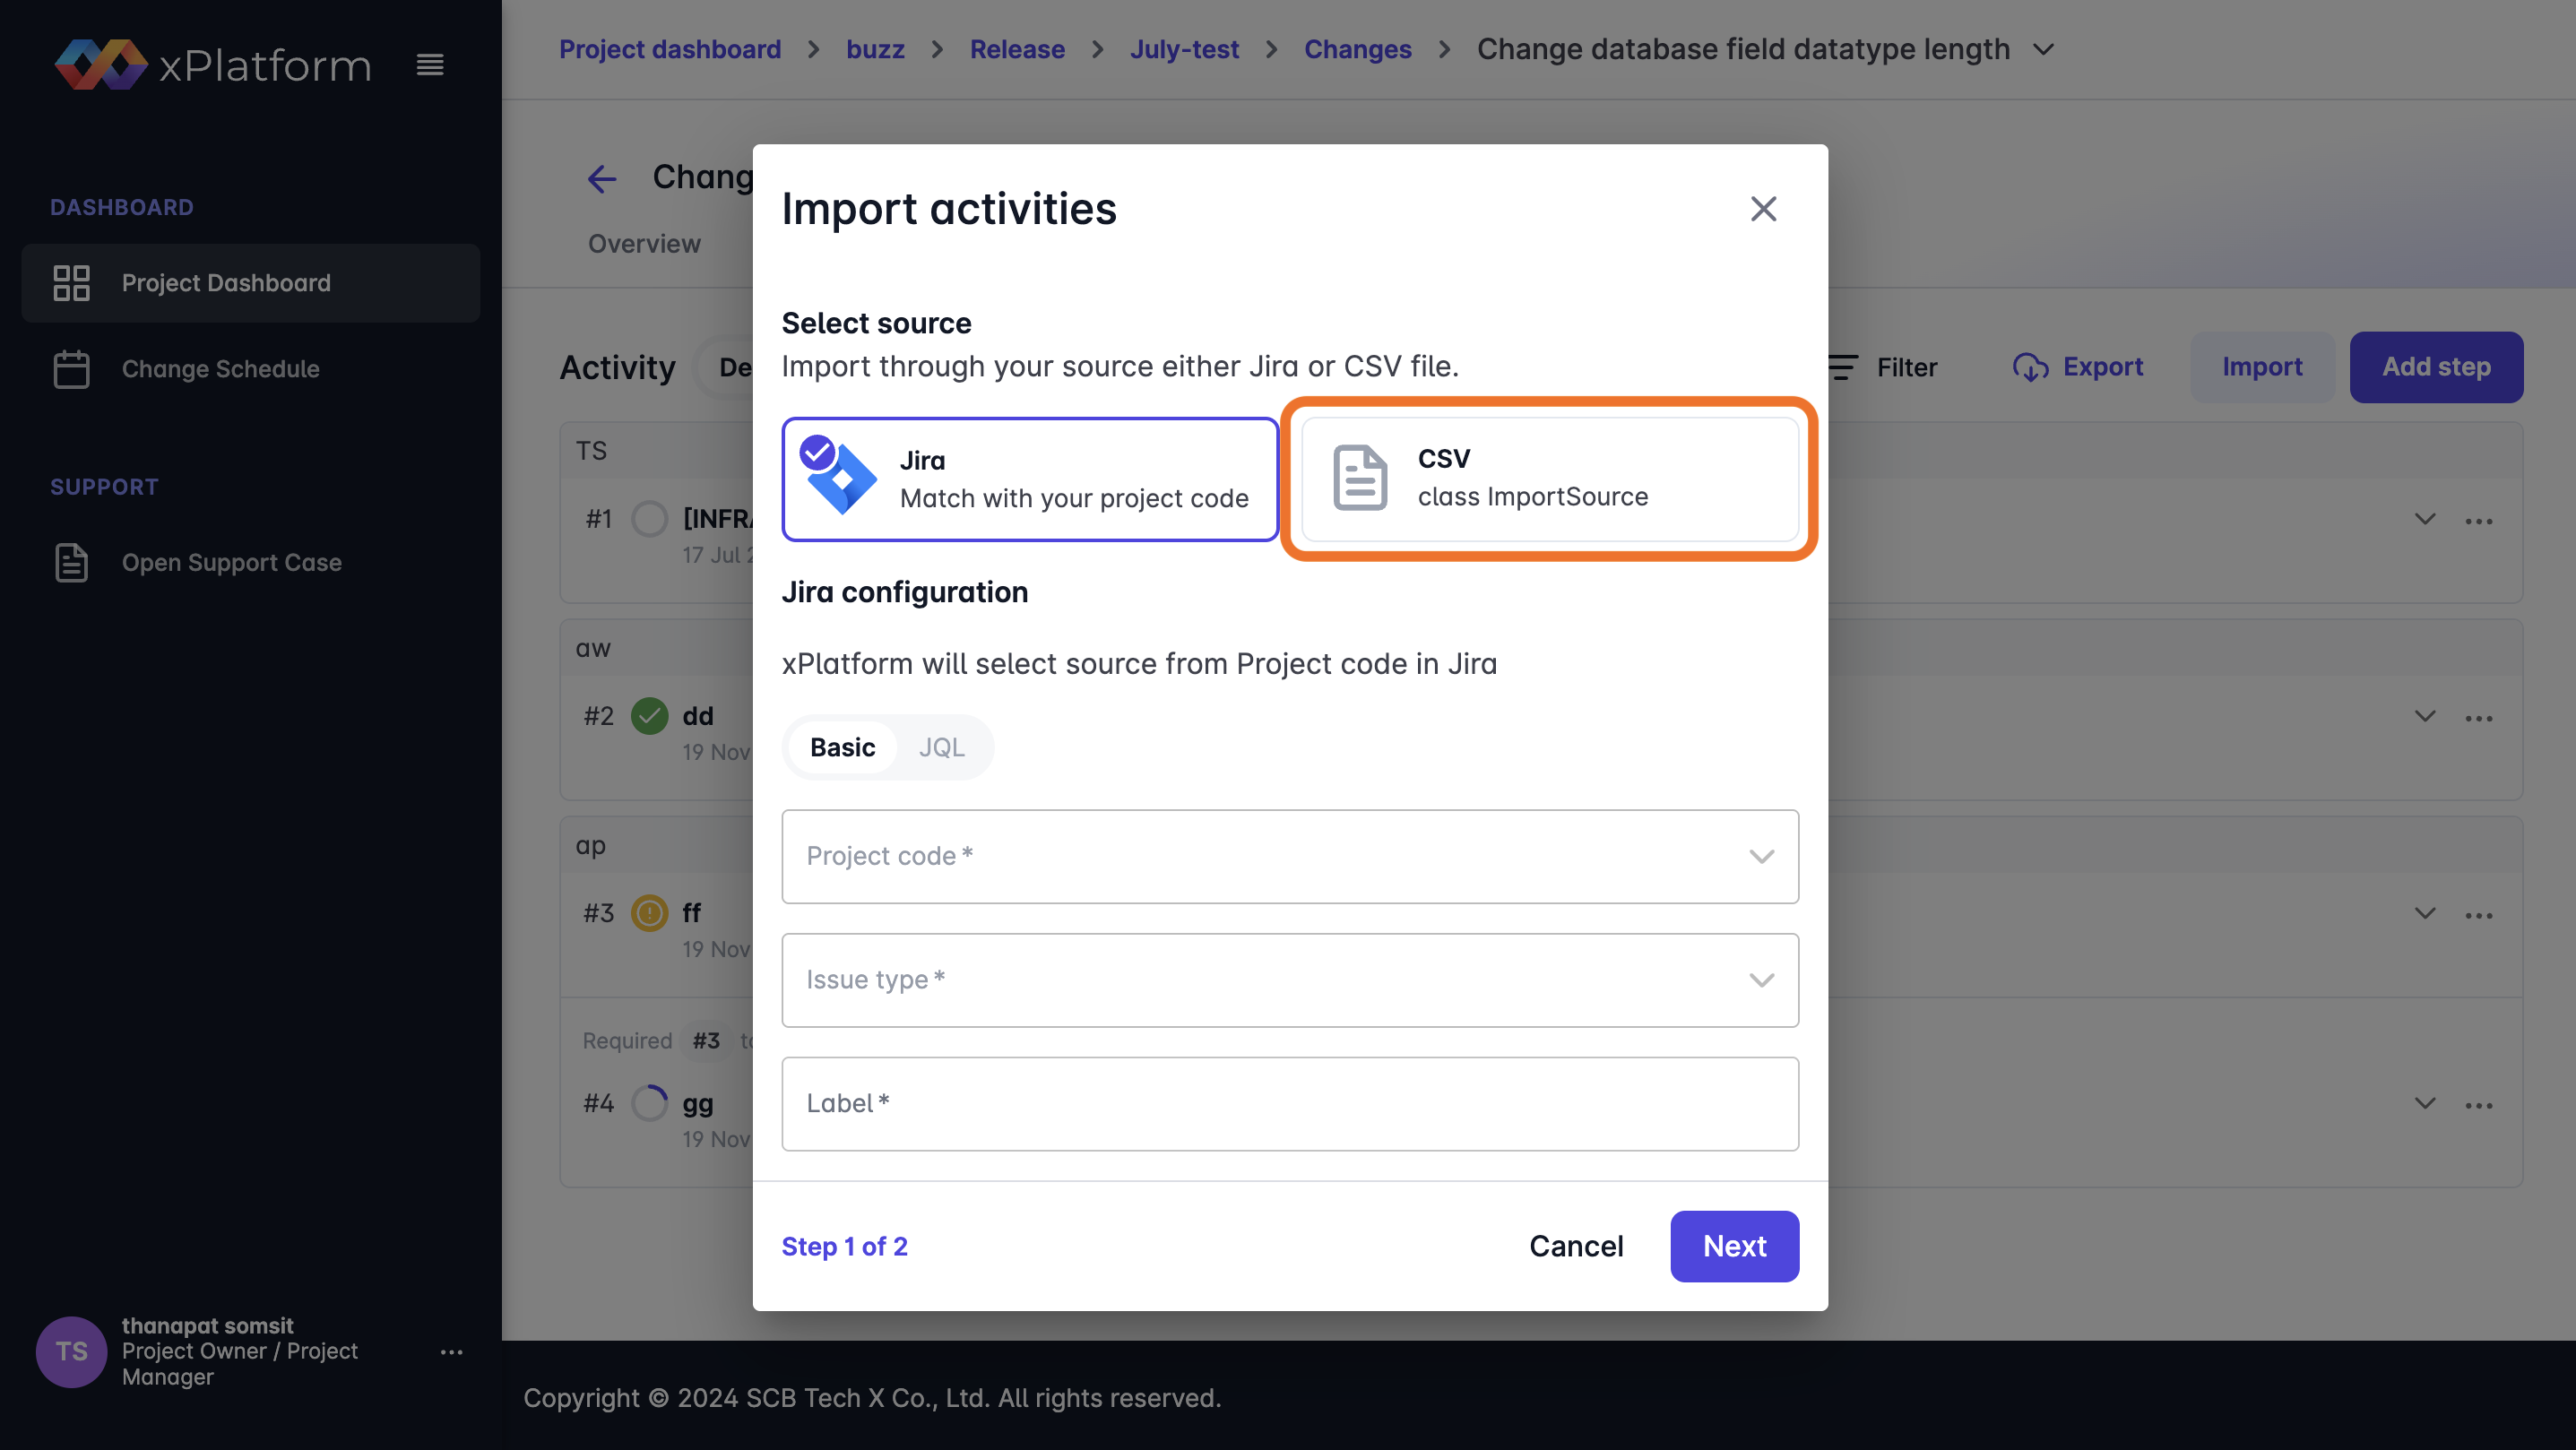
\includegraphics[width=\linewidth]{resources/pages/change-runbook/import-csv/31.png}

    \vspace{1in}

    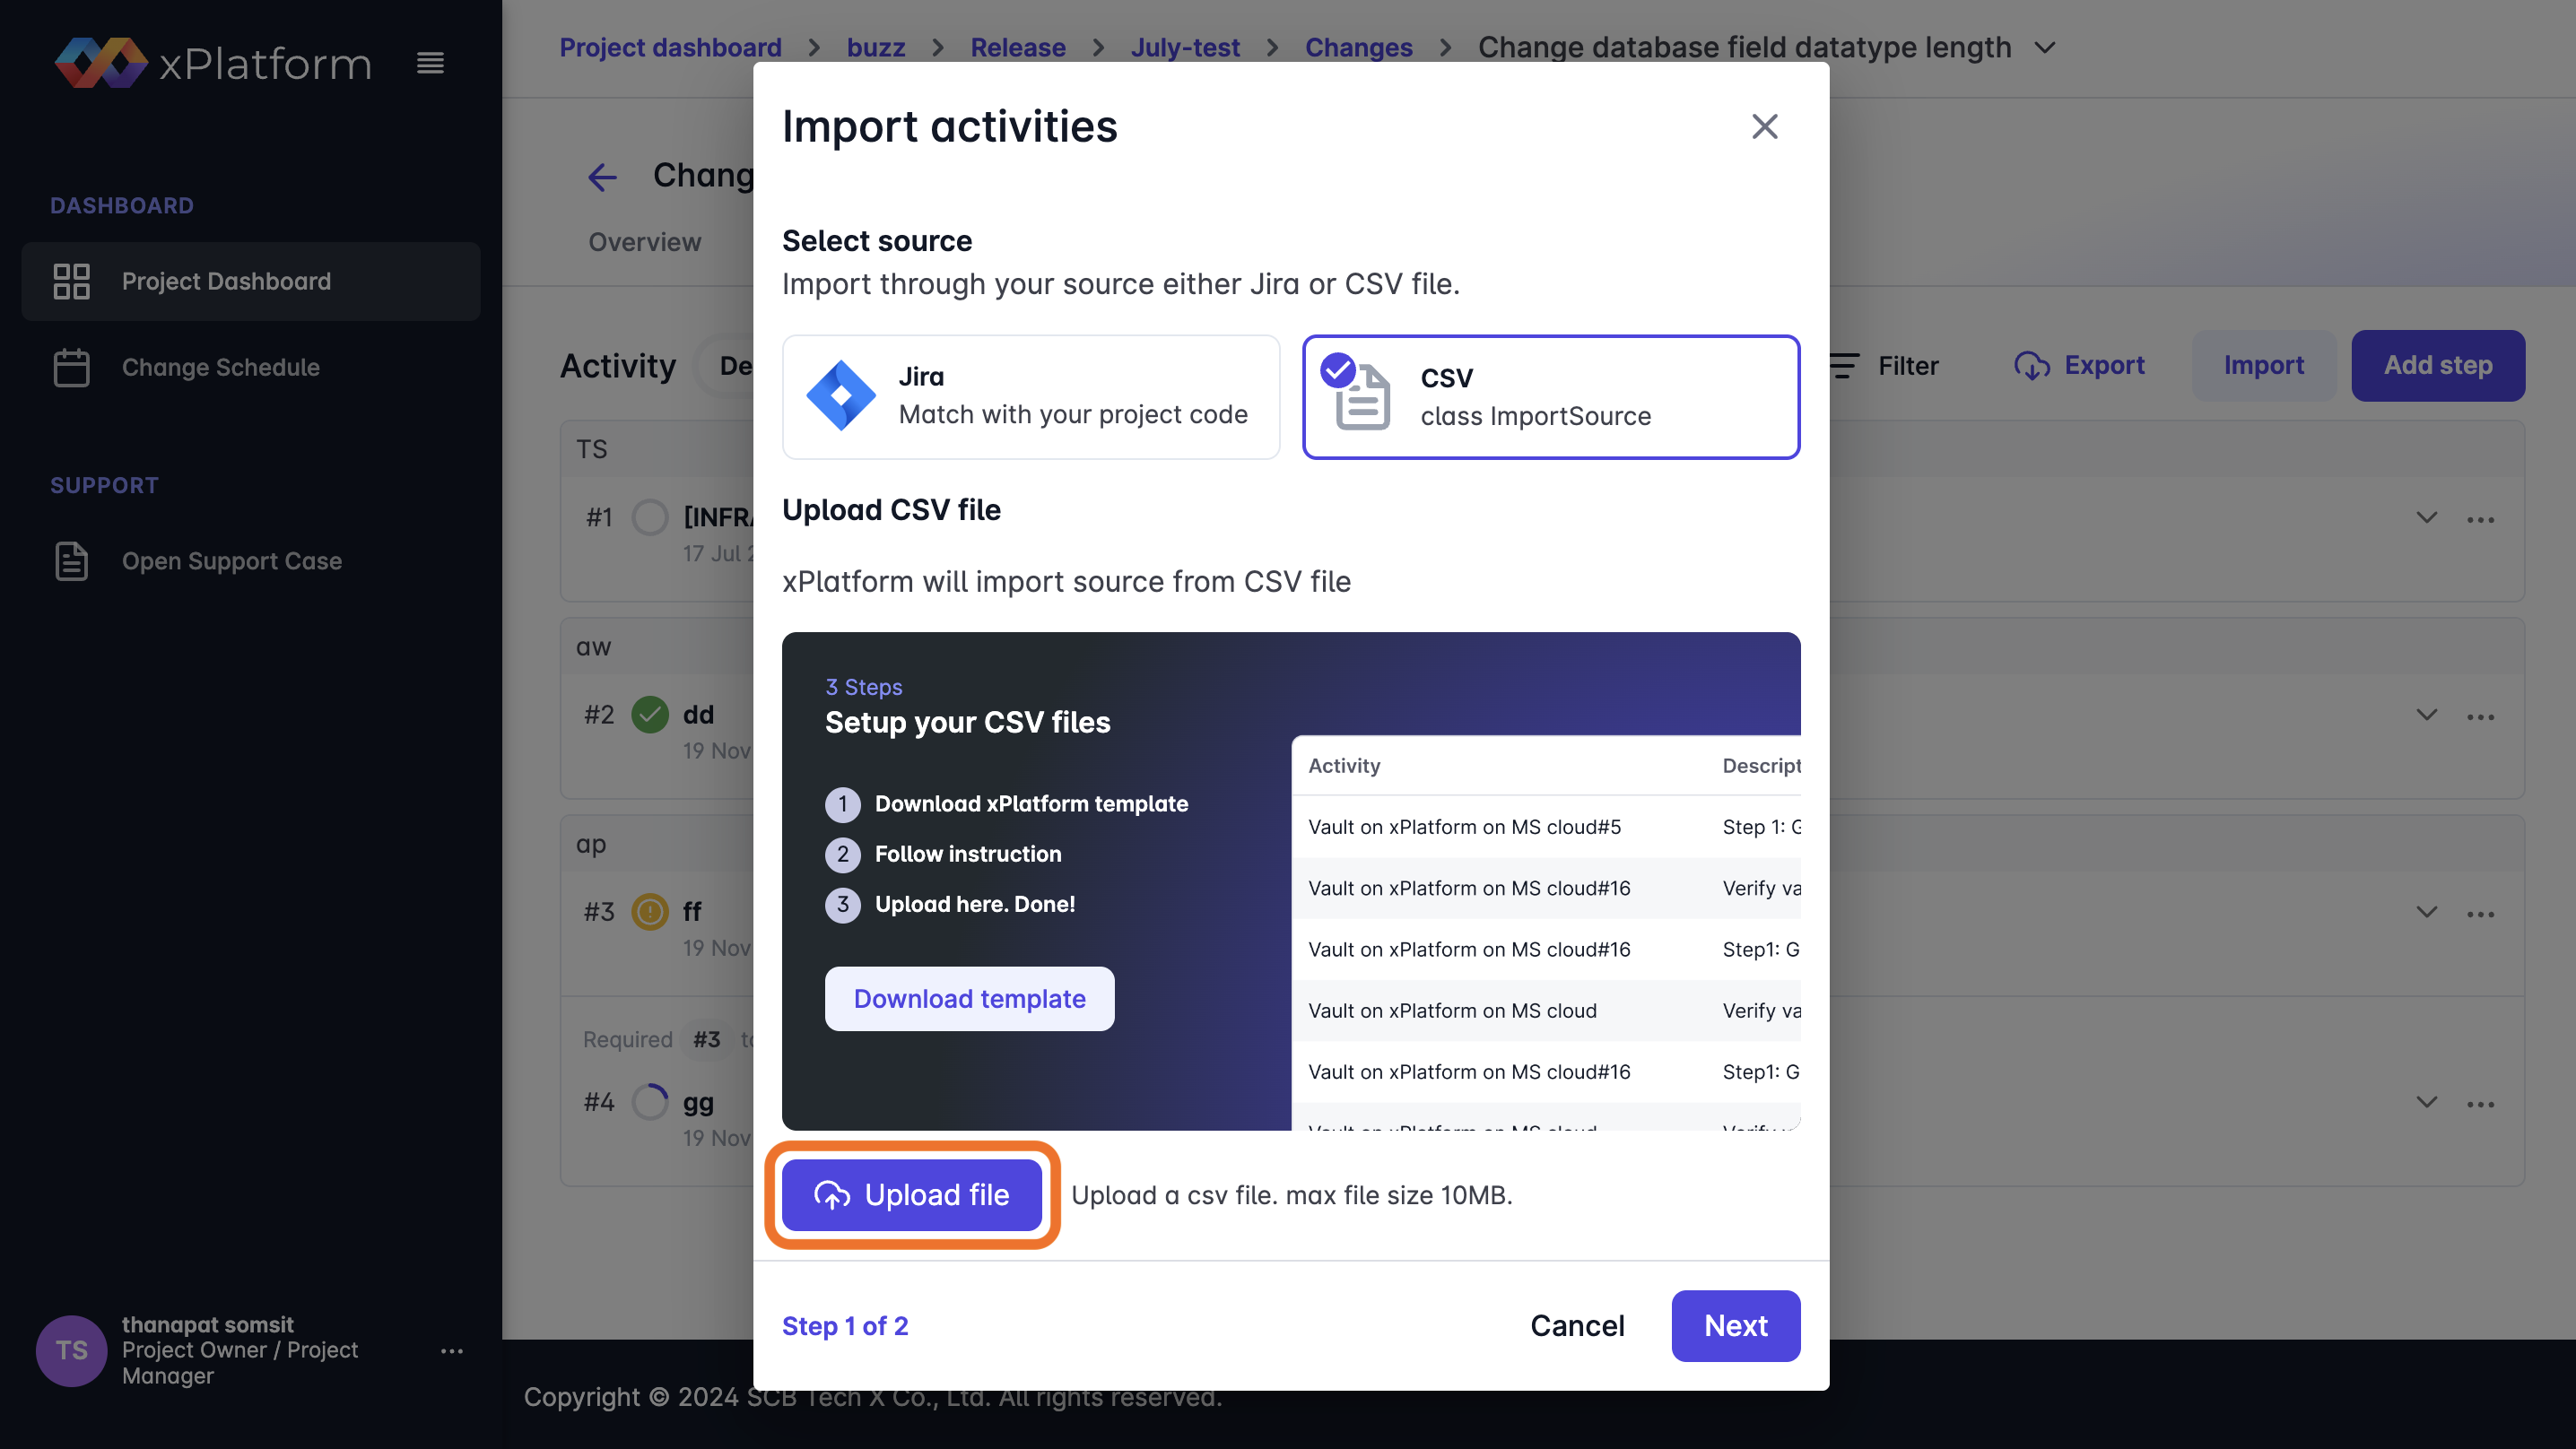
\includegraphics[width=\linewidth]{resources/pages/change-runbook/import-csv/32.png}
\end{center}
\begin{center}
    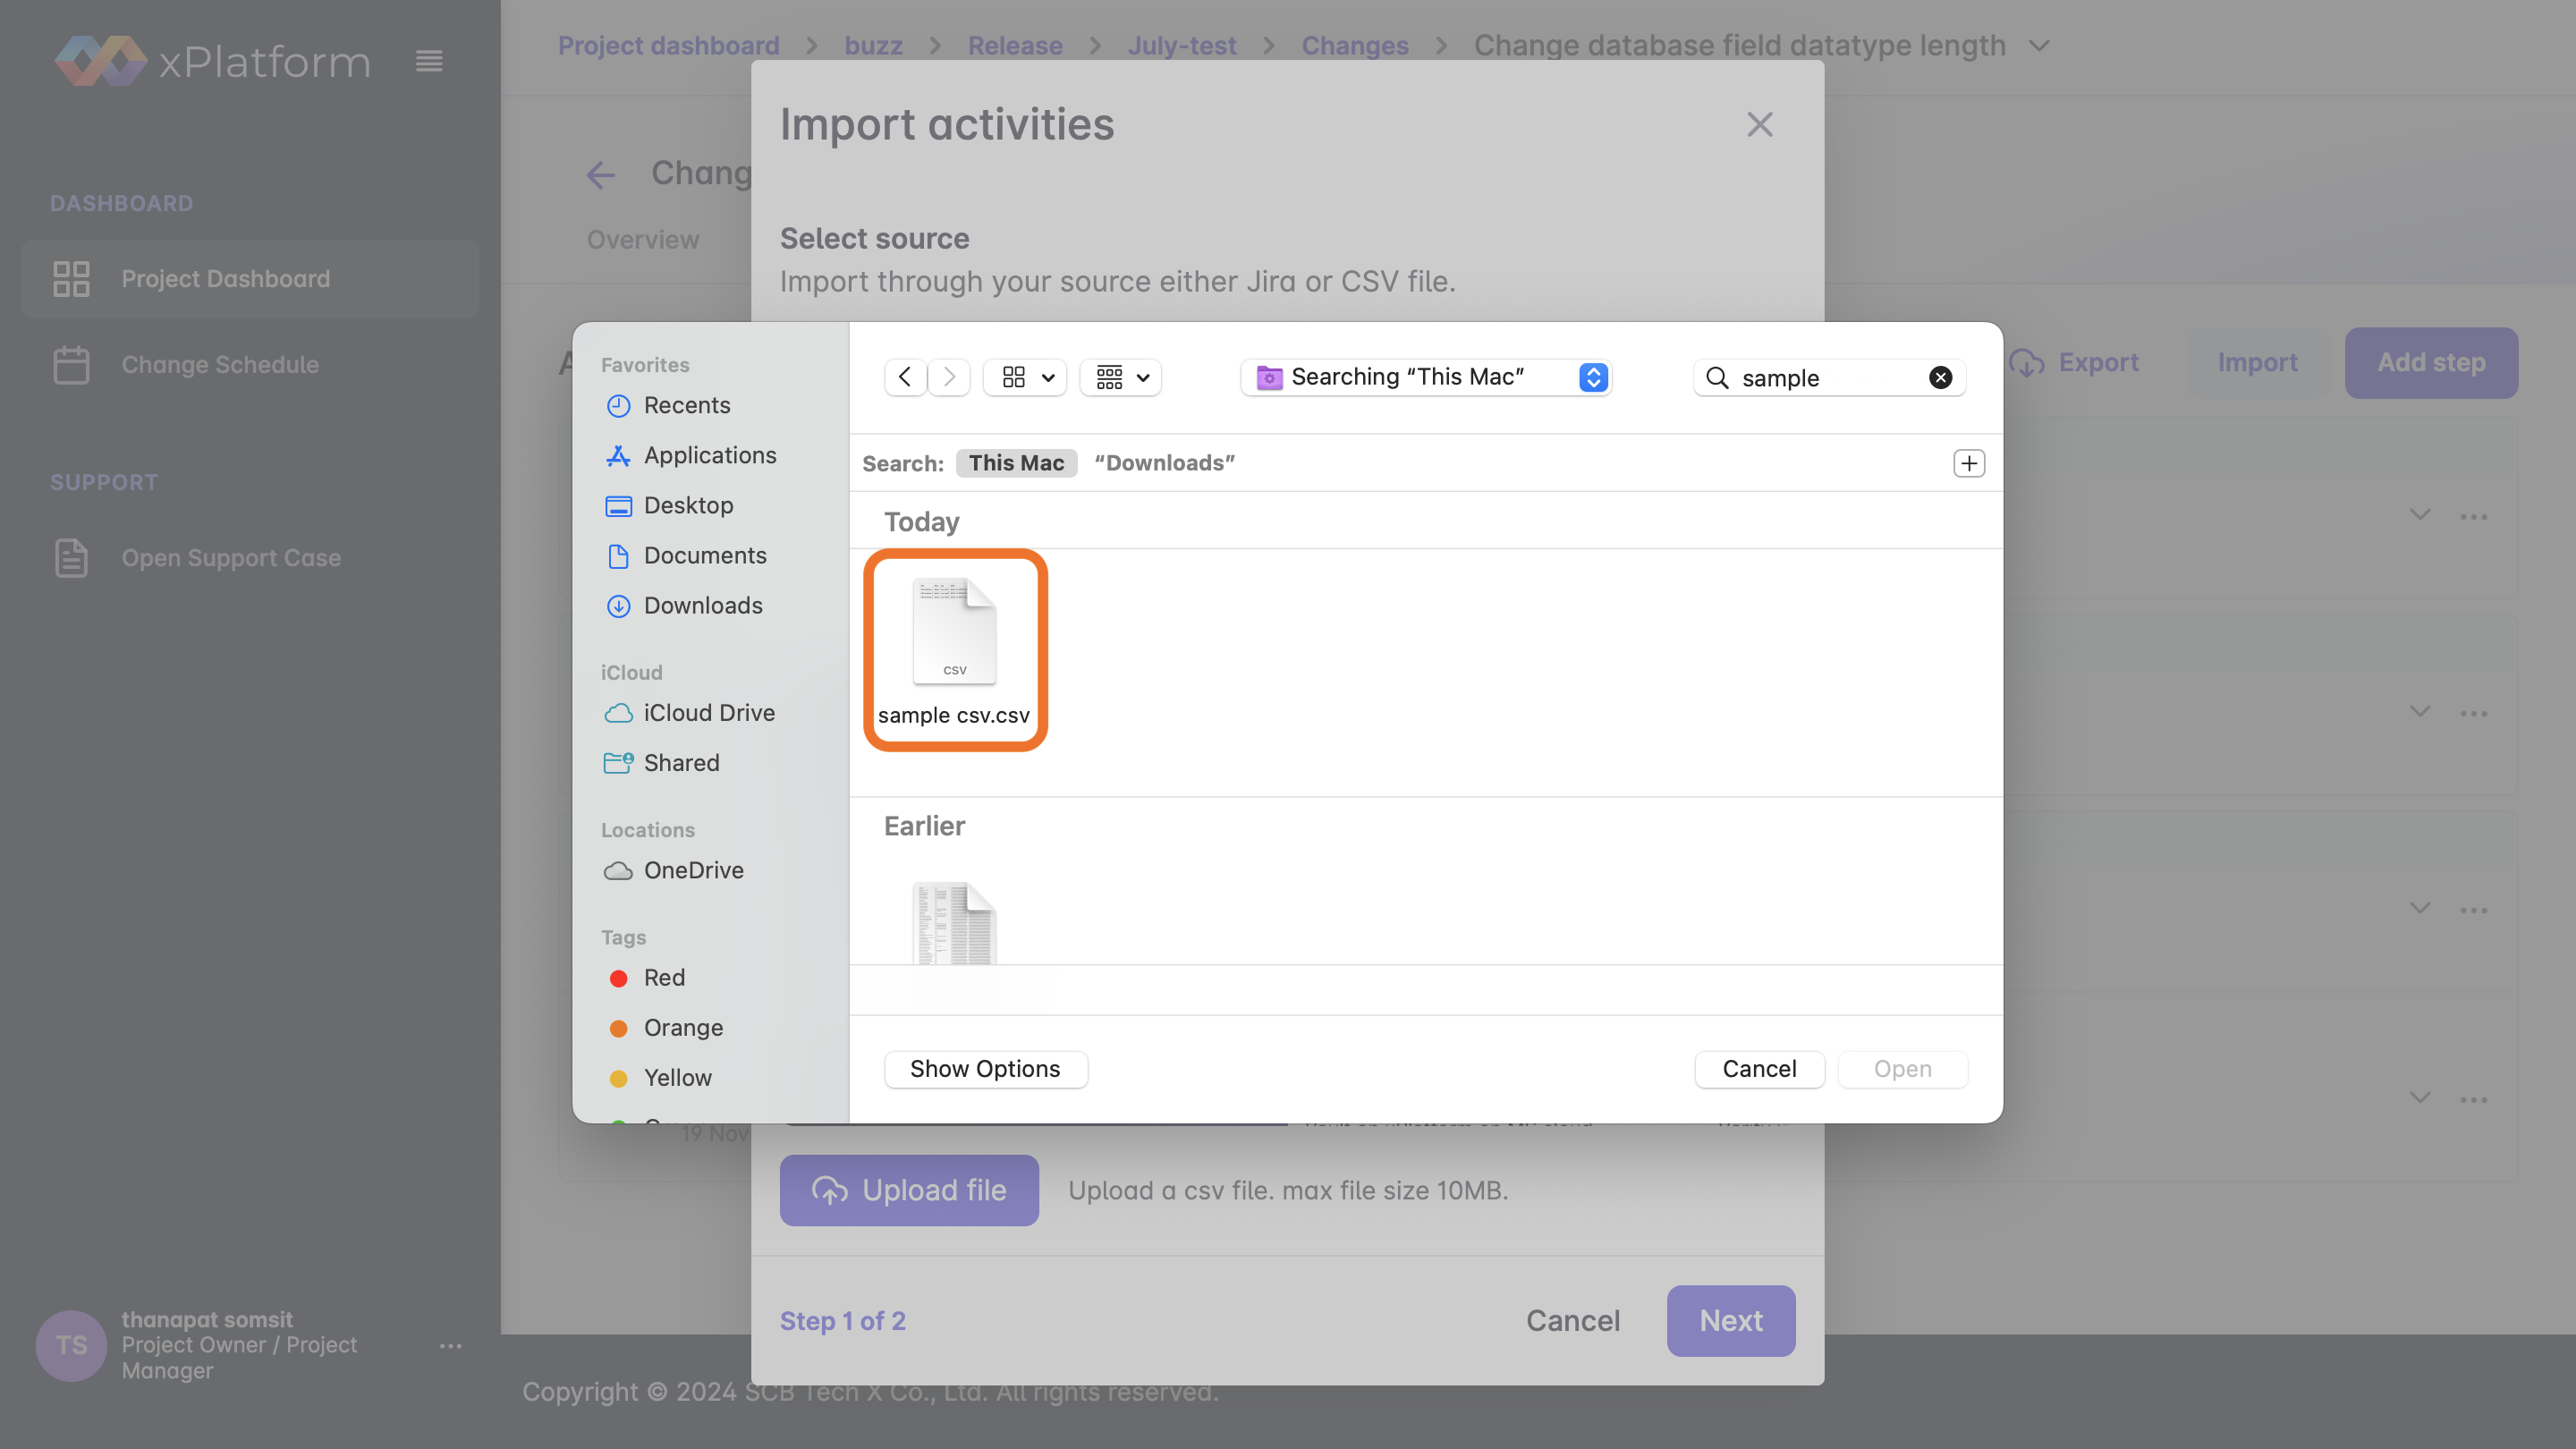
\includegraphics[width=\linewidth]{resources/pages/change-runbook/import-csv/33.png}

    \vspace{1in}

    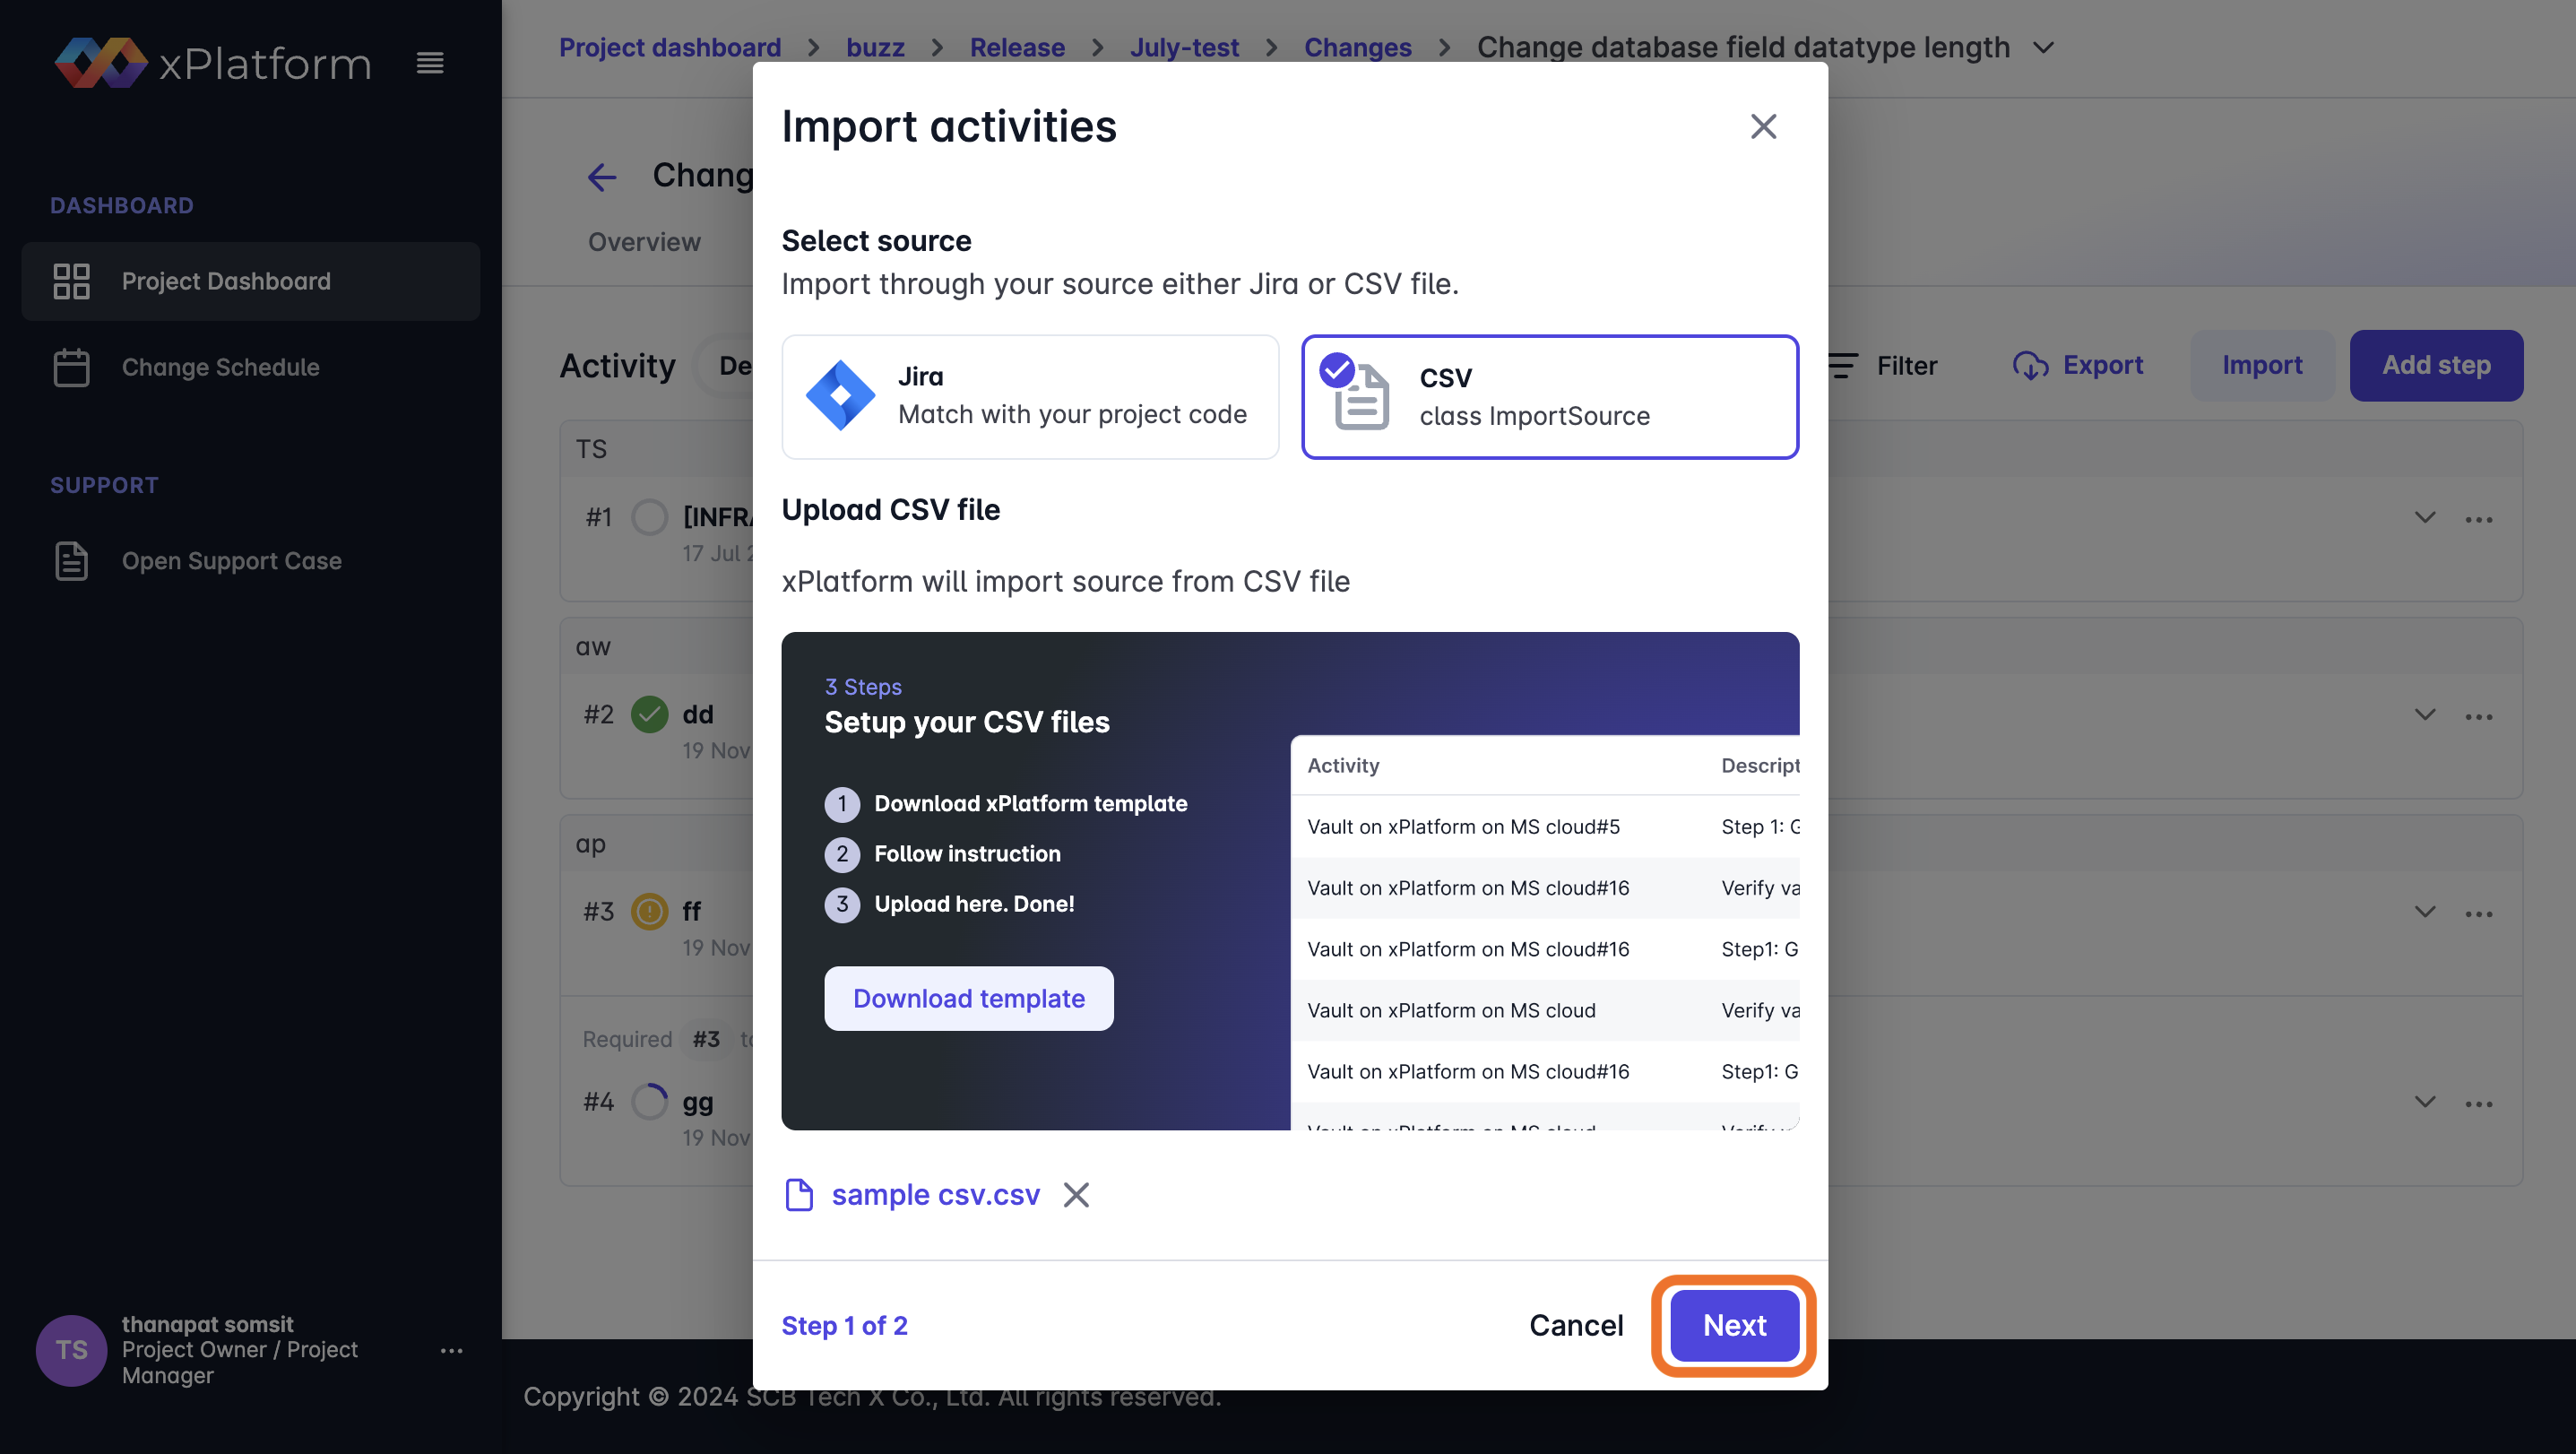
\includegraphics[width=\linewidth]{resources/pages/change-runbook/import-csv/34.png}
\end{center}
\begin{center}
    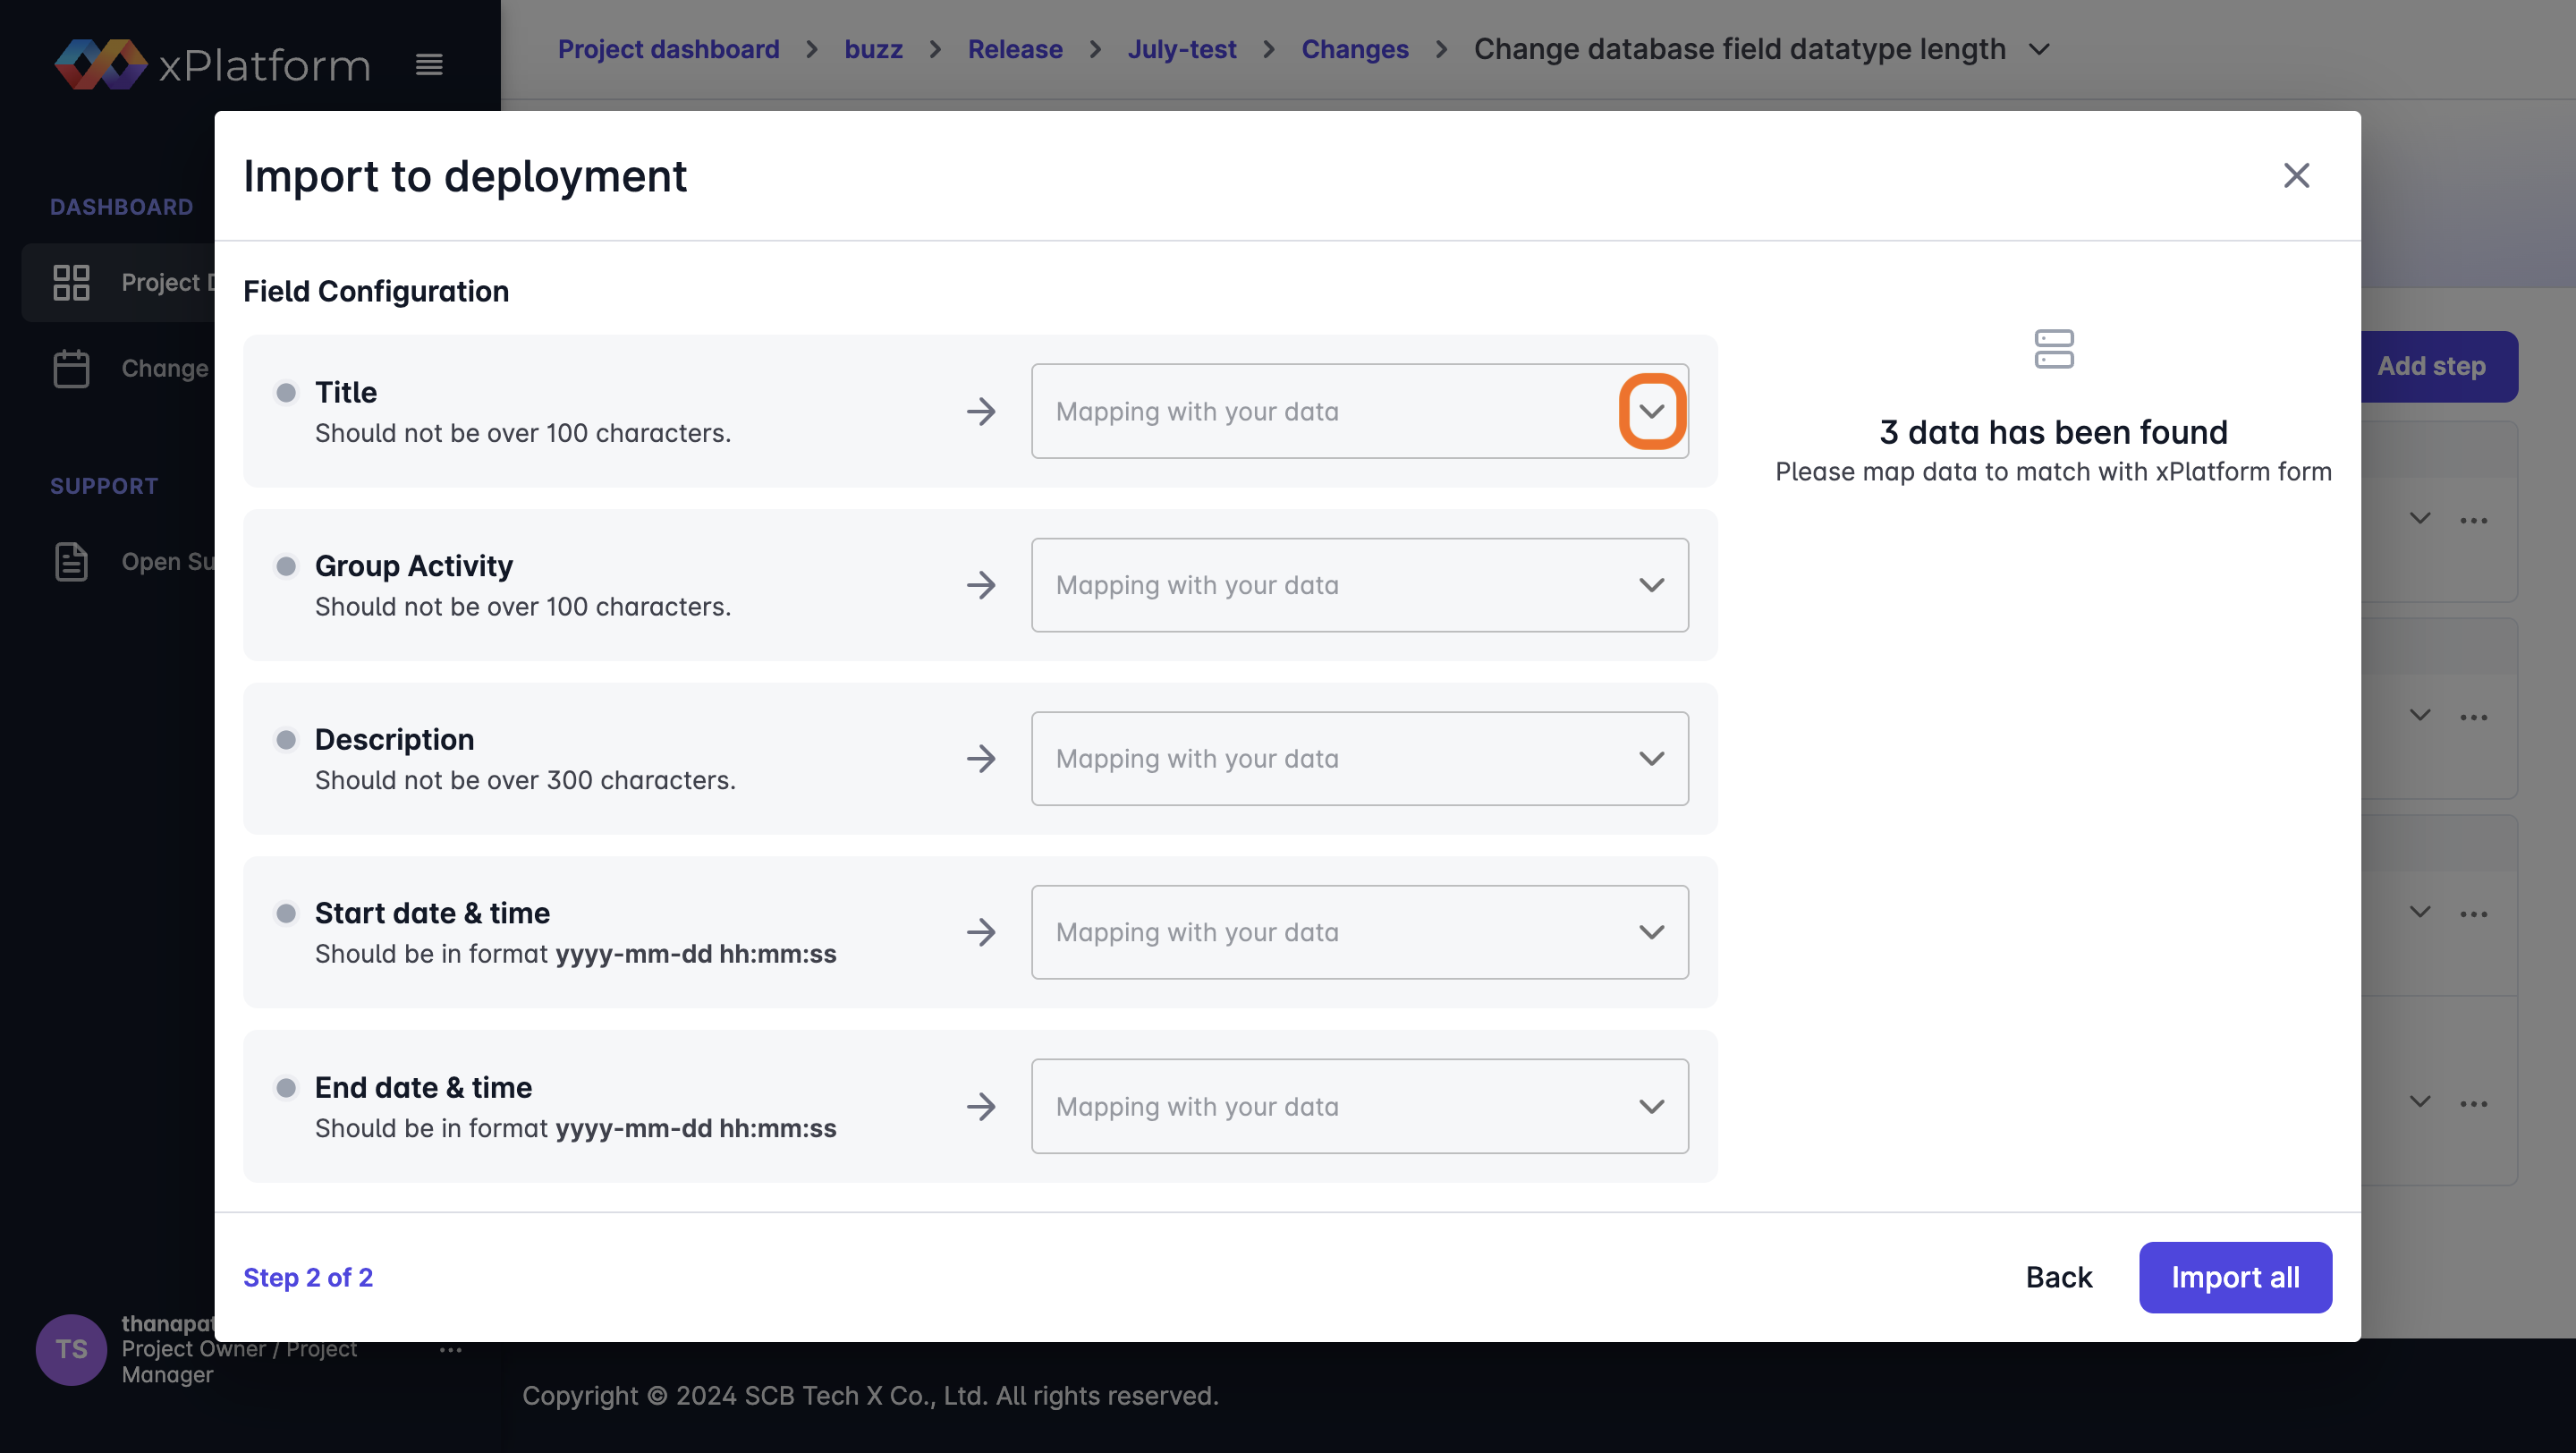
\includegraphics[width=\linewidth]{resources/pages/change-runbook/import-csv/35.png}

    \vspace{1in}

    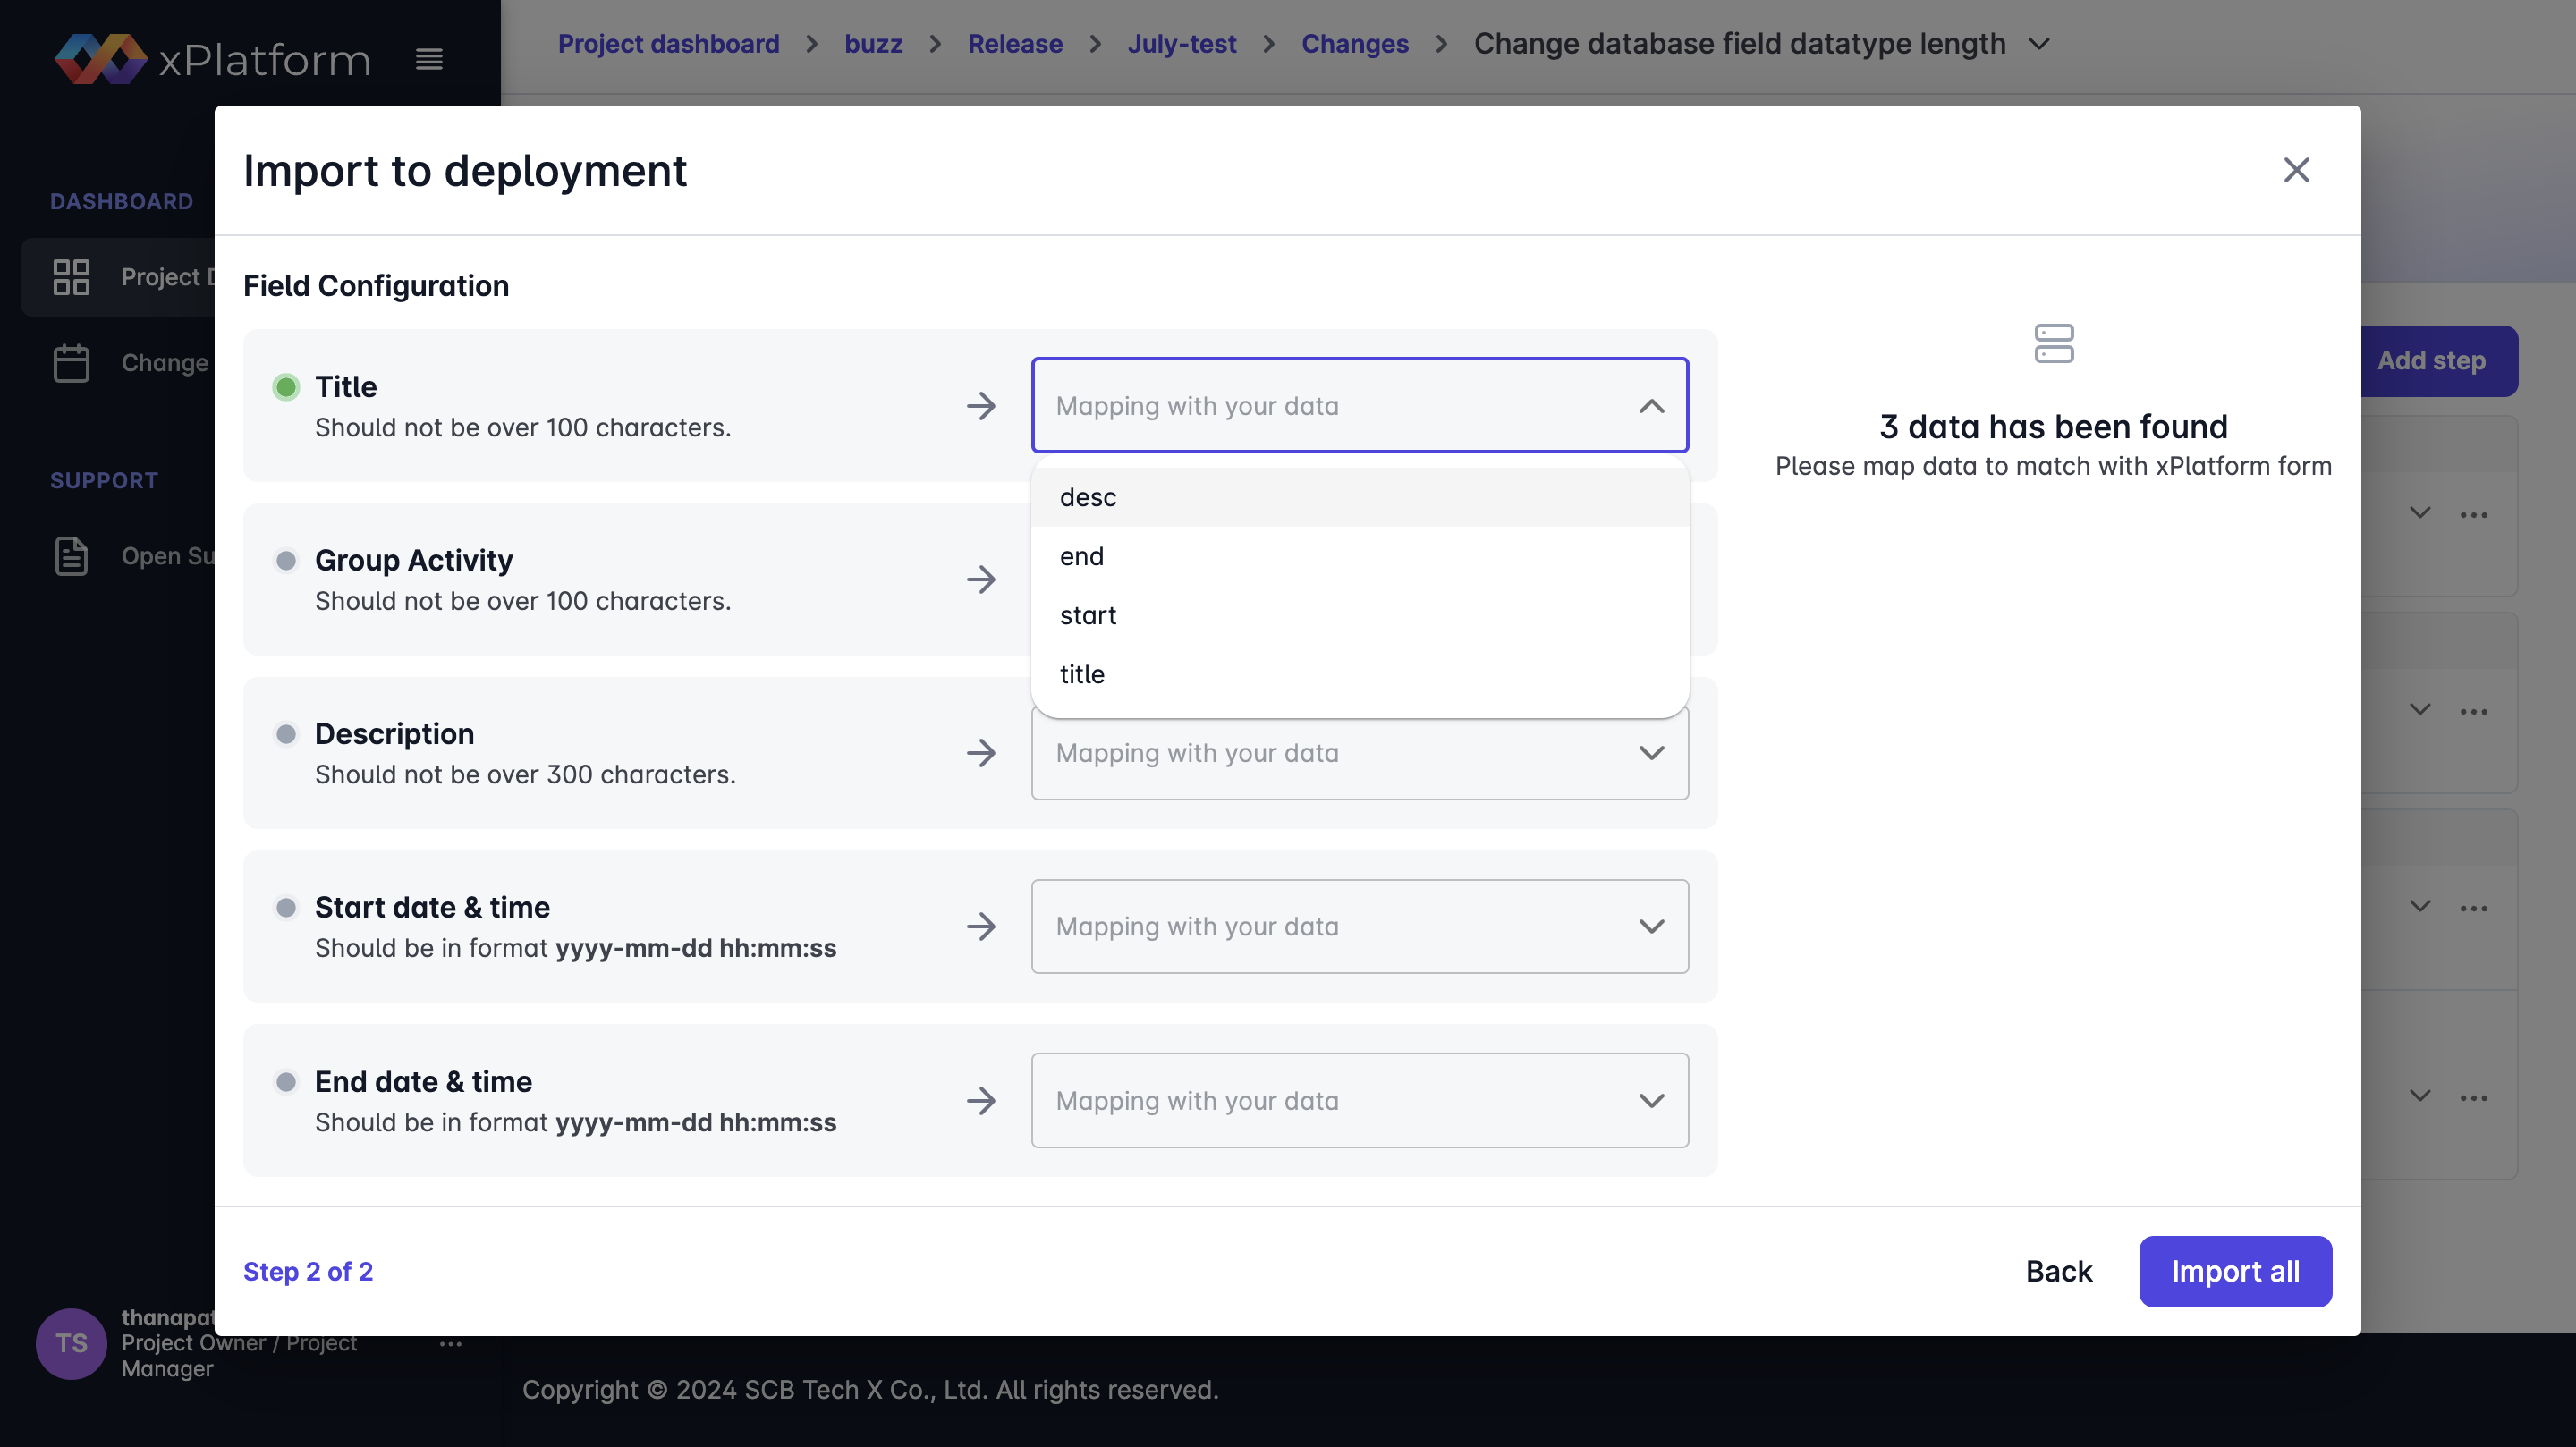
\includegraphics[width=\linewidth]{resources/pages/change-runbook/import-csv/36.png}
\end{center}

\begin{figure}[H]
    \begin{center}
        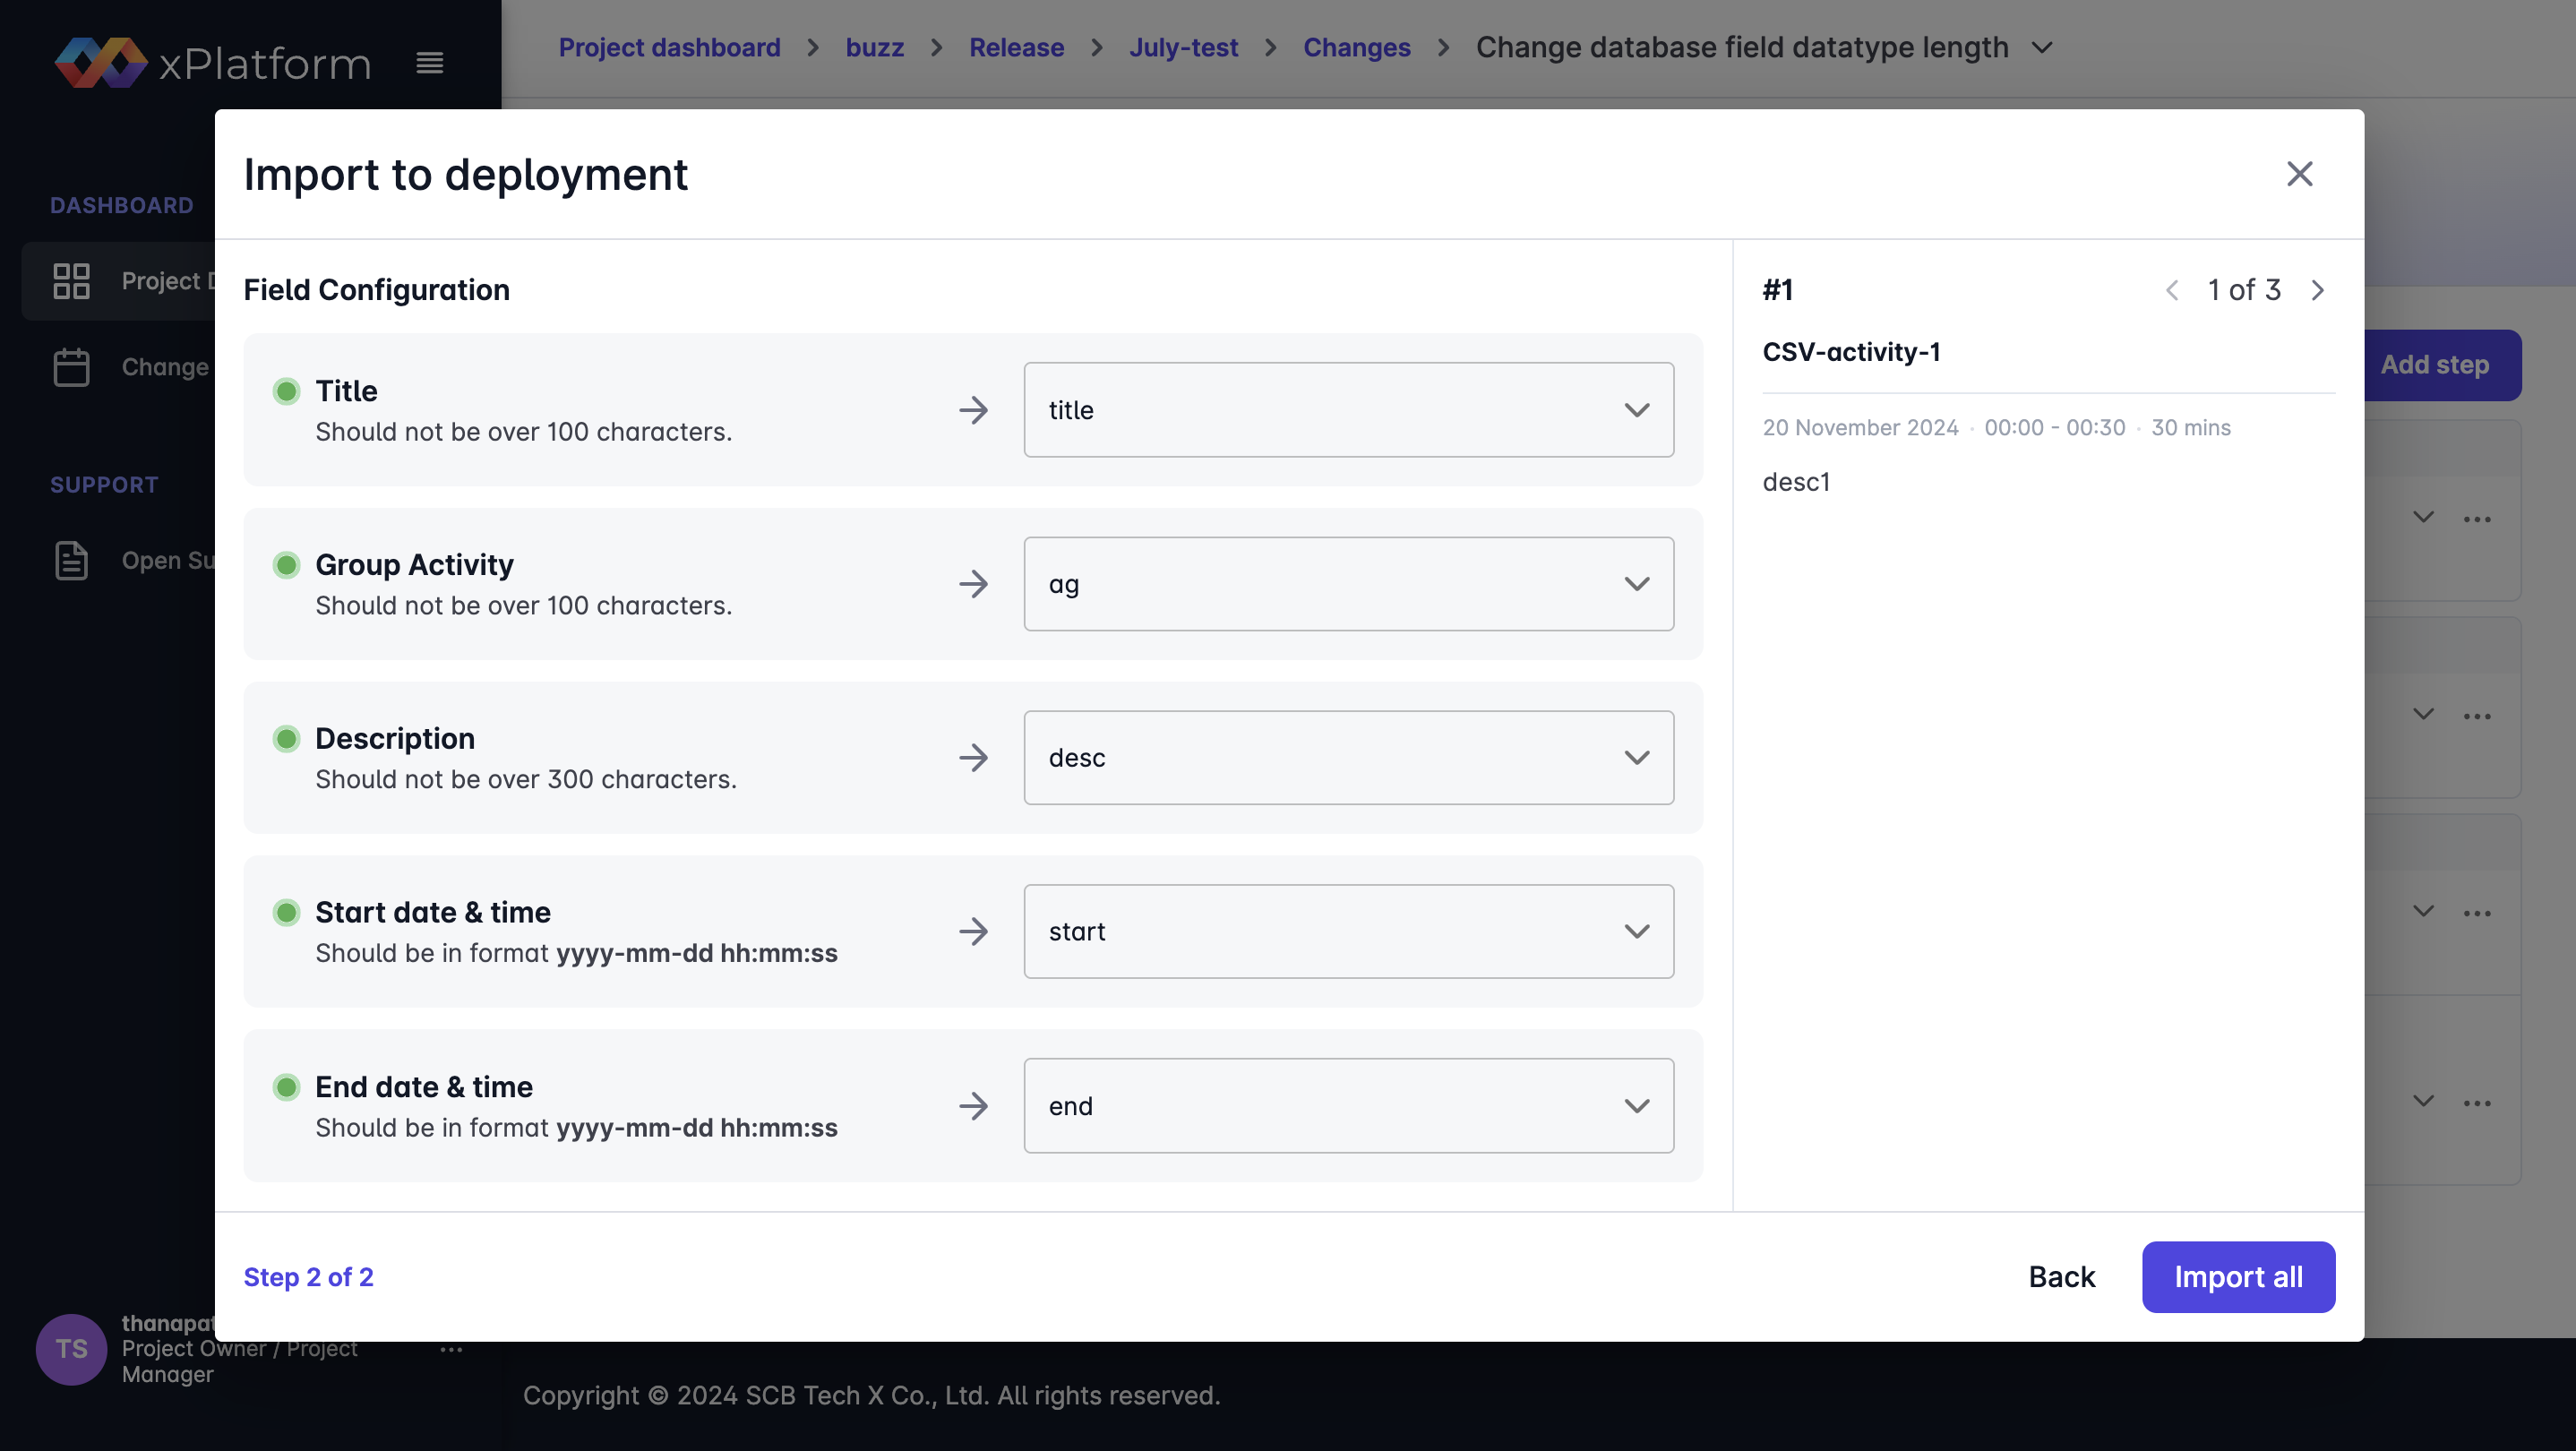
\includegraphics[width=\linewidth]{resources/pages/change-runbook/import-csv/37.png}
    
        \vspace{1in}
    
        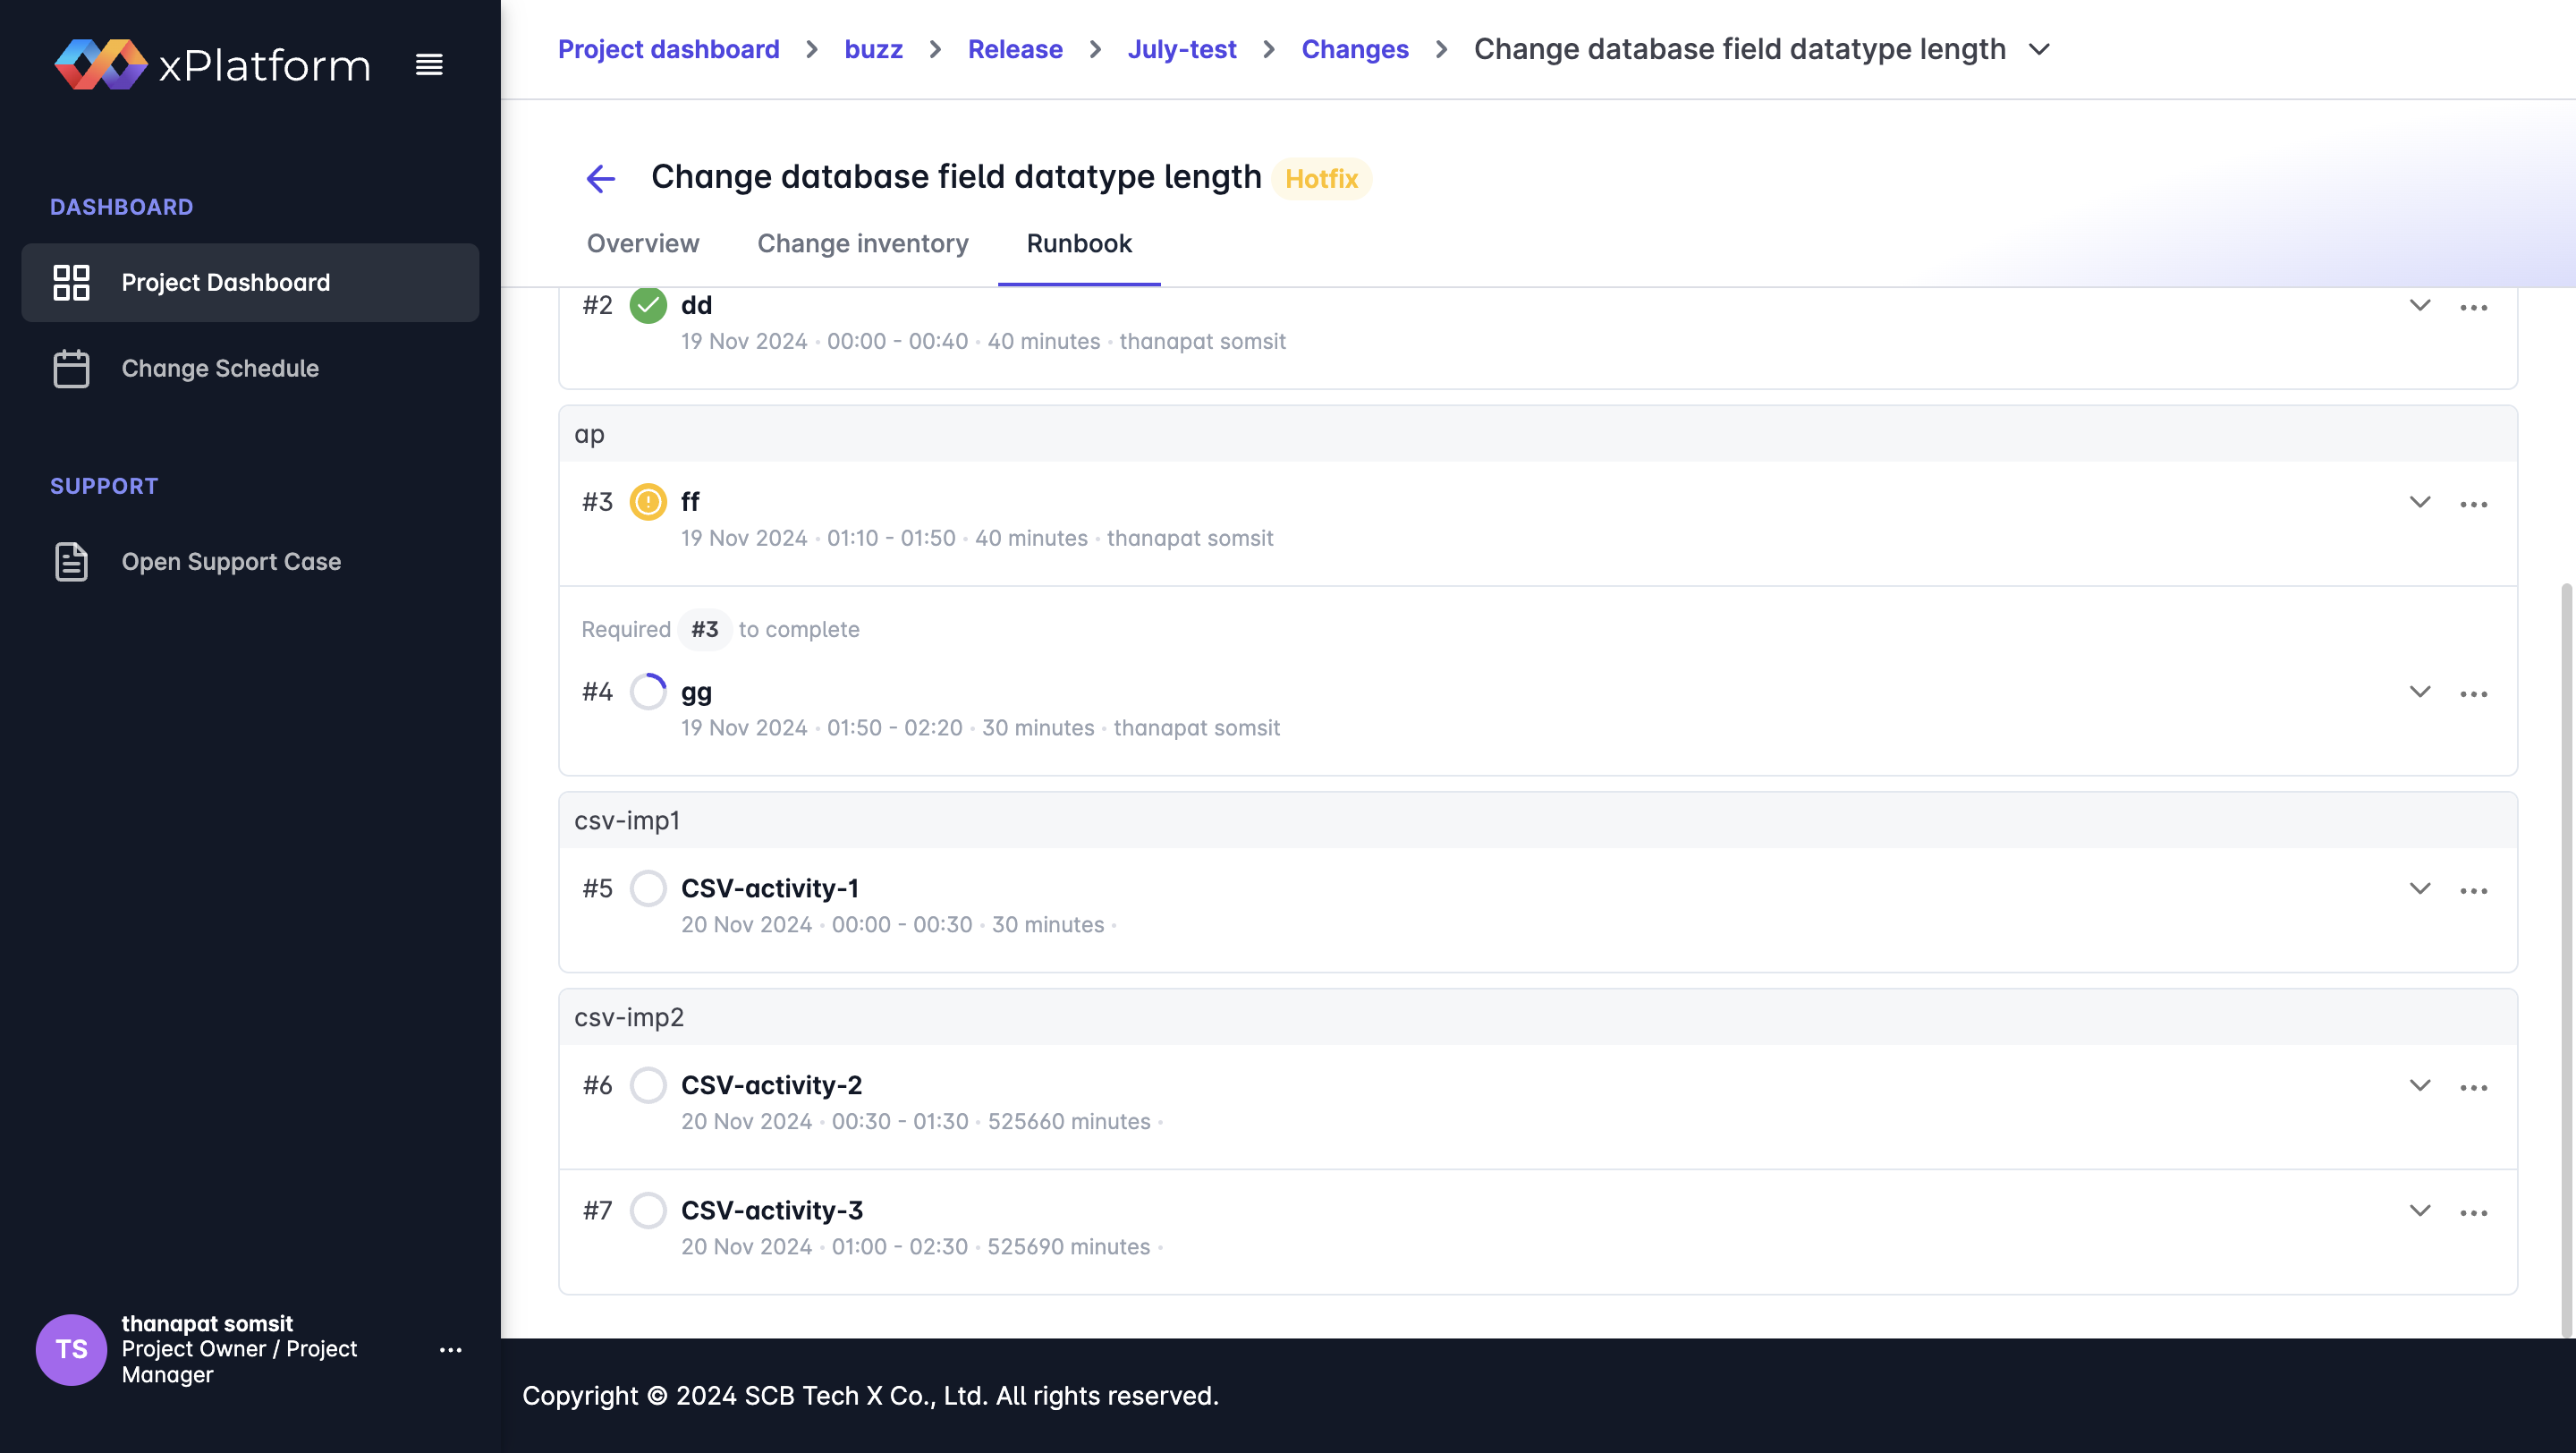
\includegraphics[width=\linewidth]{resources/pages/change-runbook/import-csv/38.png}
    \end{center}
    \caption[การดึงข้อมูลจาก CSV]{การดึงข้อมูลจาก CSV}
  \label{fig:import-csv}
\end{figure}

\newpage
\subsection{การดูข้อมูล Change Runbook ด้วย Gantt Chart}
\begin{figure}[H]
    \begin{center}
        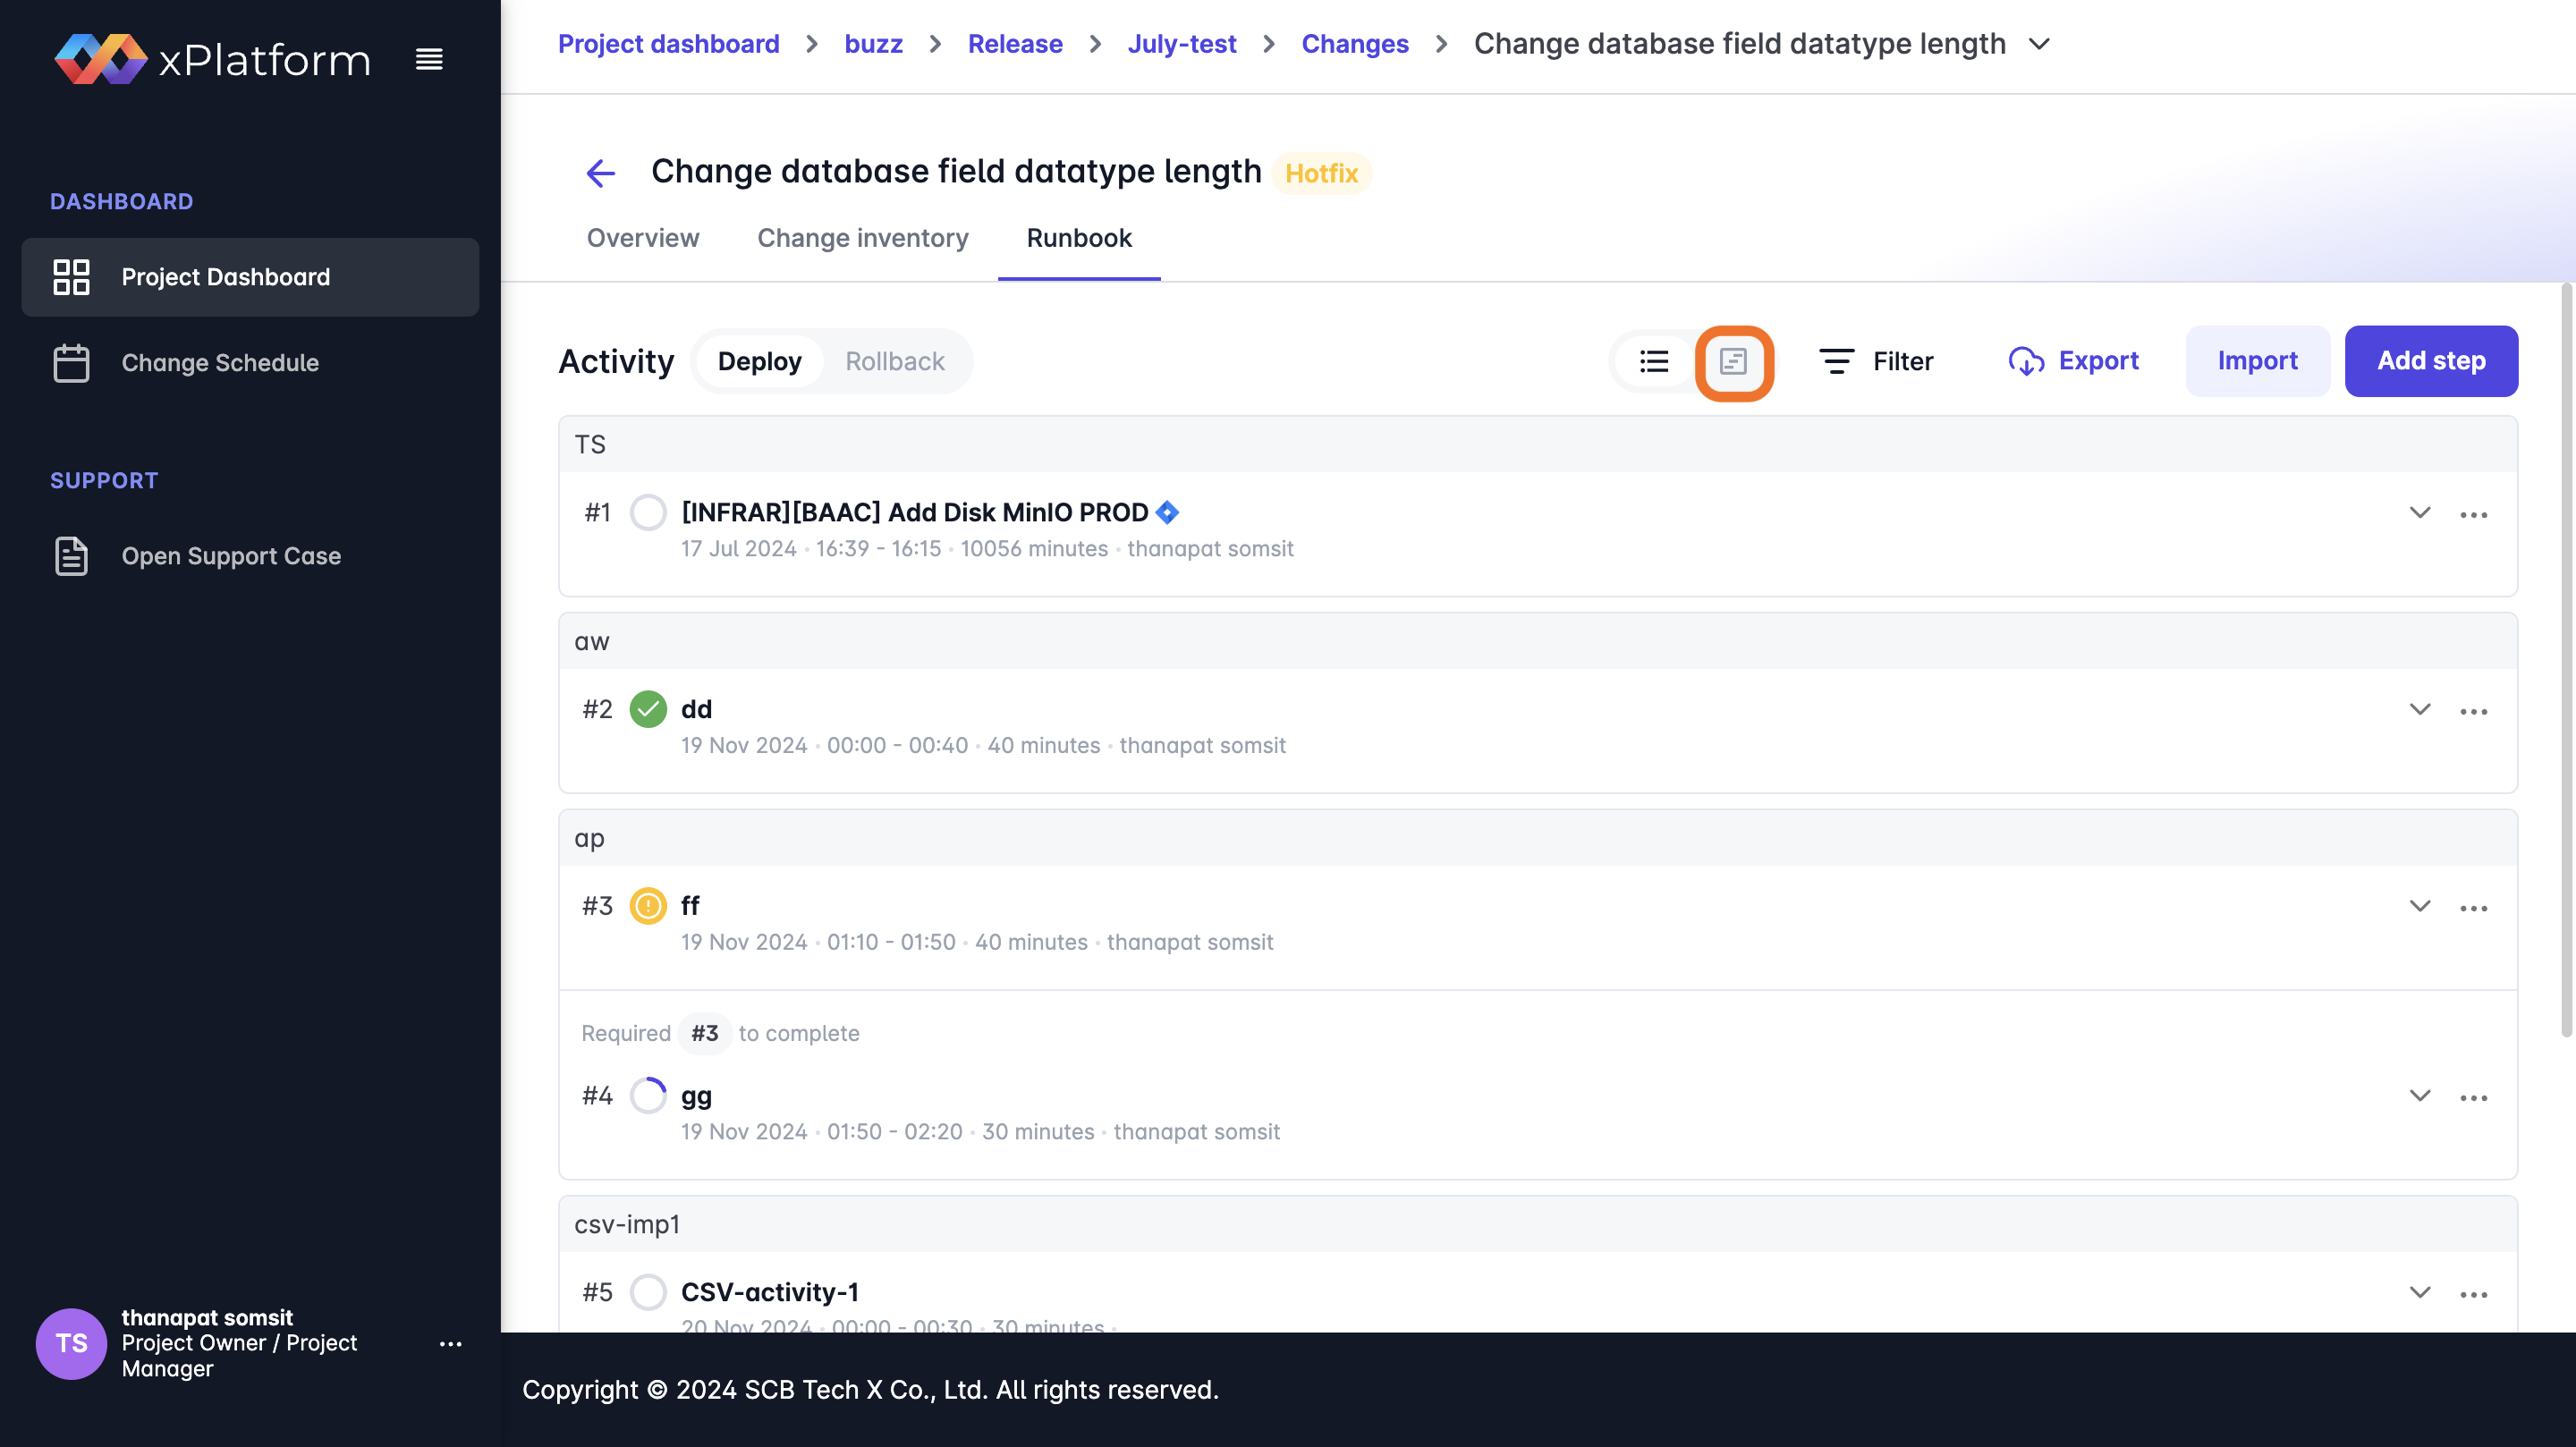
\includegraphics[width=\linewidth]{resources/pages/change-runbook/gantt-chart/39.png}
    
        \vspace{1in}
    
        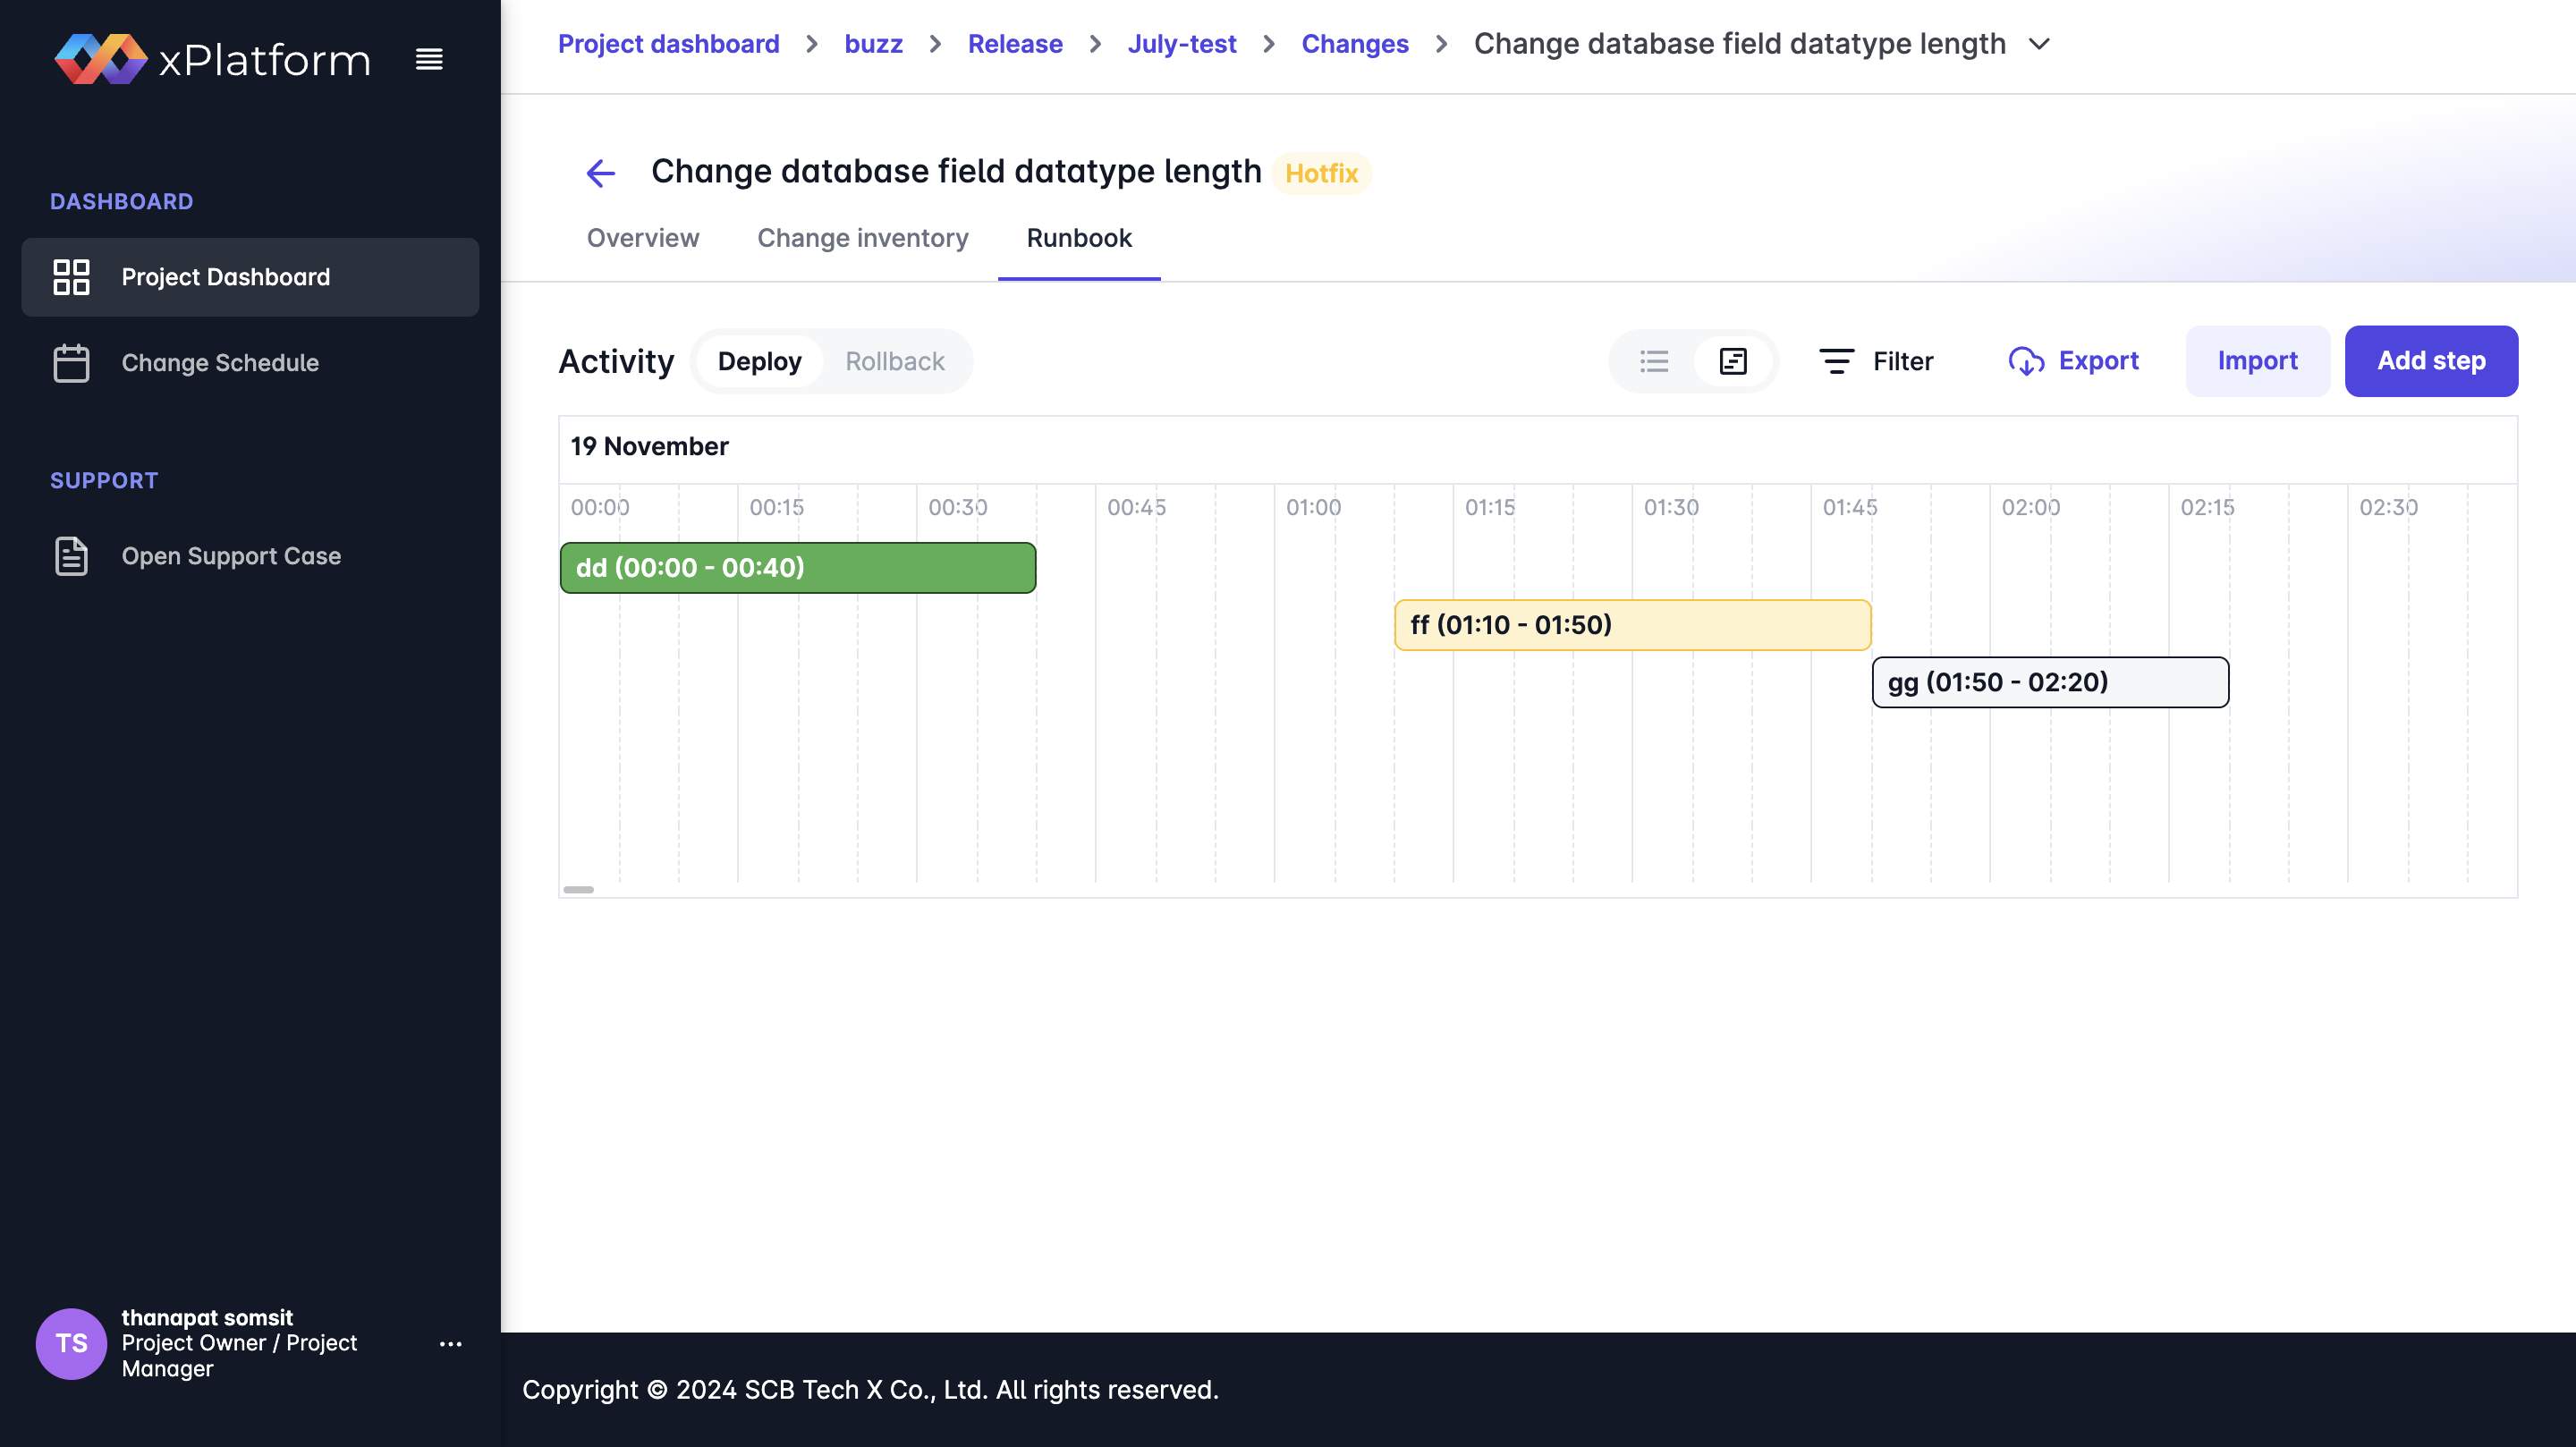
\includegraphics[width=\linewidth]{resources/pages/change-runbook/gantt-chart/40.png}
    \end{center}
    \caption[Change Runbook ด้วย Gantt Chart]{Change Runbook ด้วย Gantt Chart}
  \label{fig:gantt-chart}
\end{figure}

\newpage
\subsection{การส่งออกไฟล์ Excel}
\begin{figure}[H]
    \begin{center}
        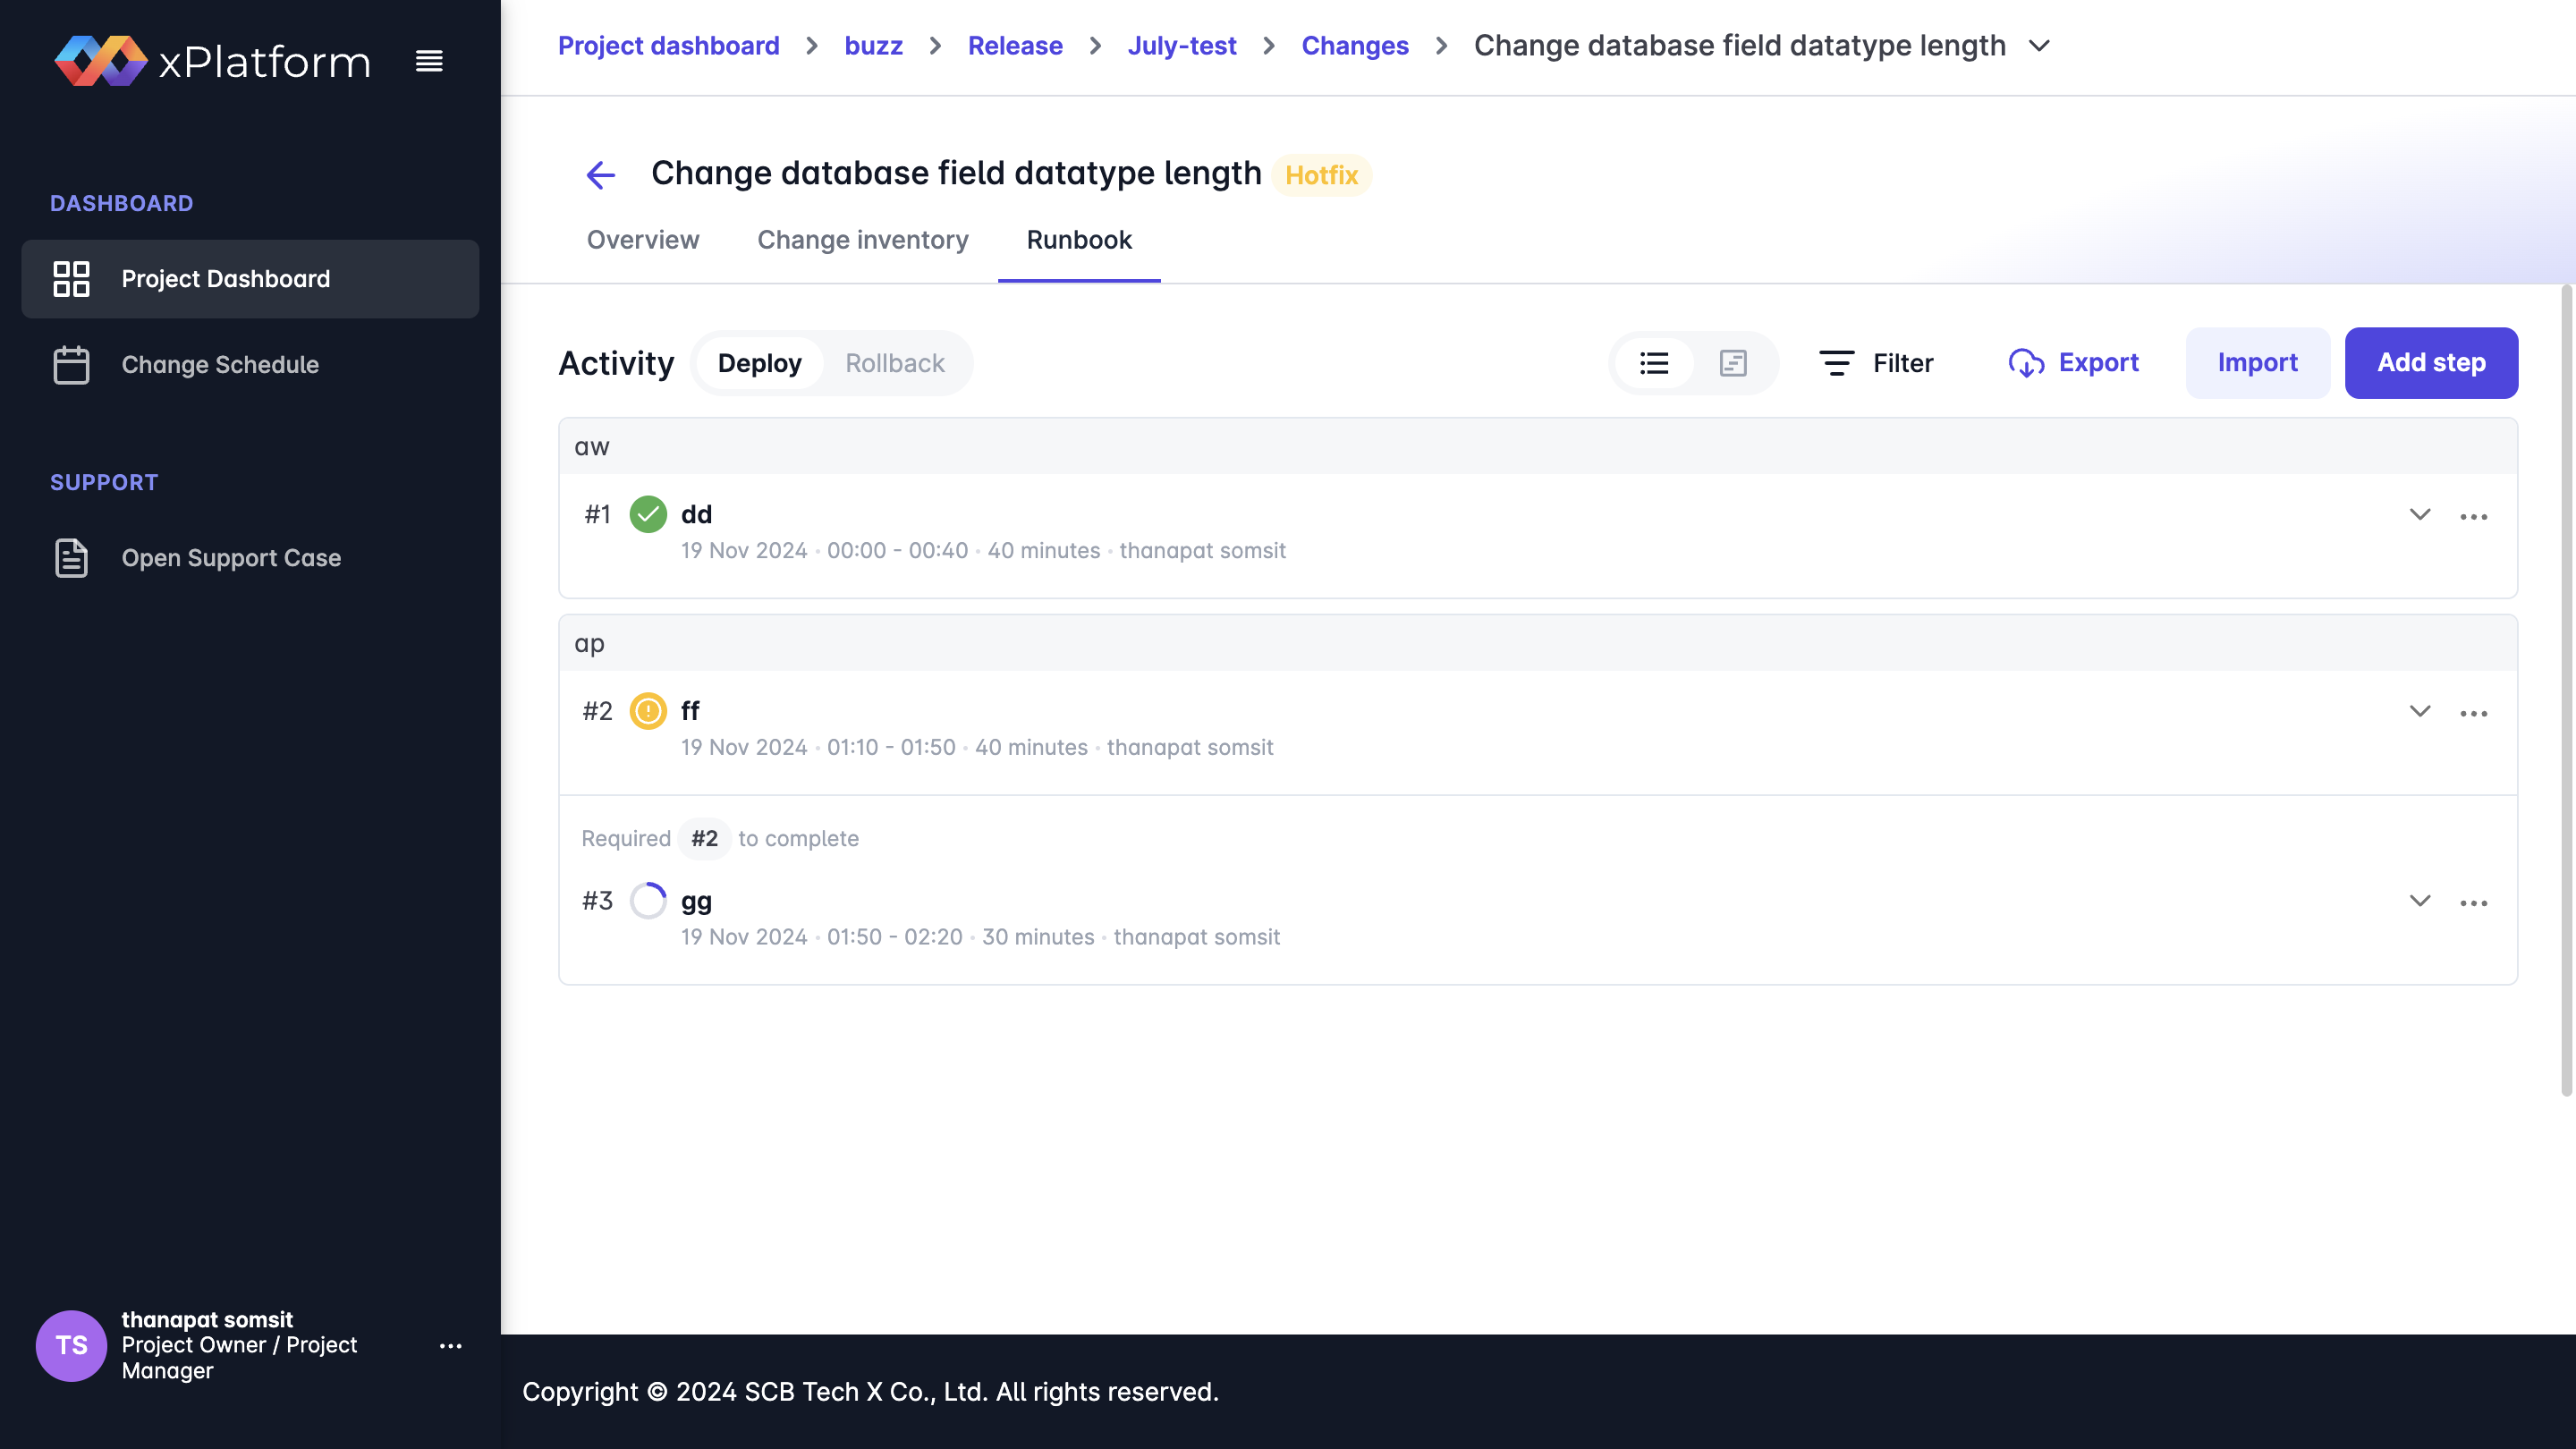
\includegraphics[width=\linewidth]{resources/pages/change-runbook/export-activity/20.png}
    
        \vspace{1in}
    
        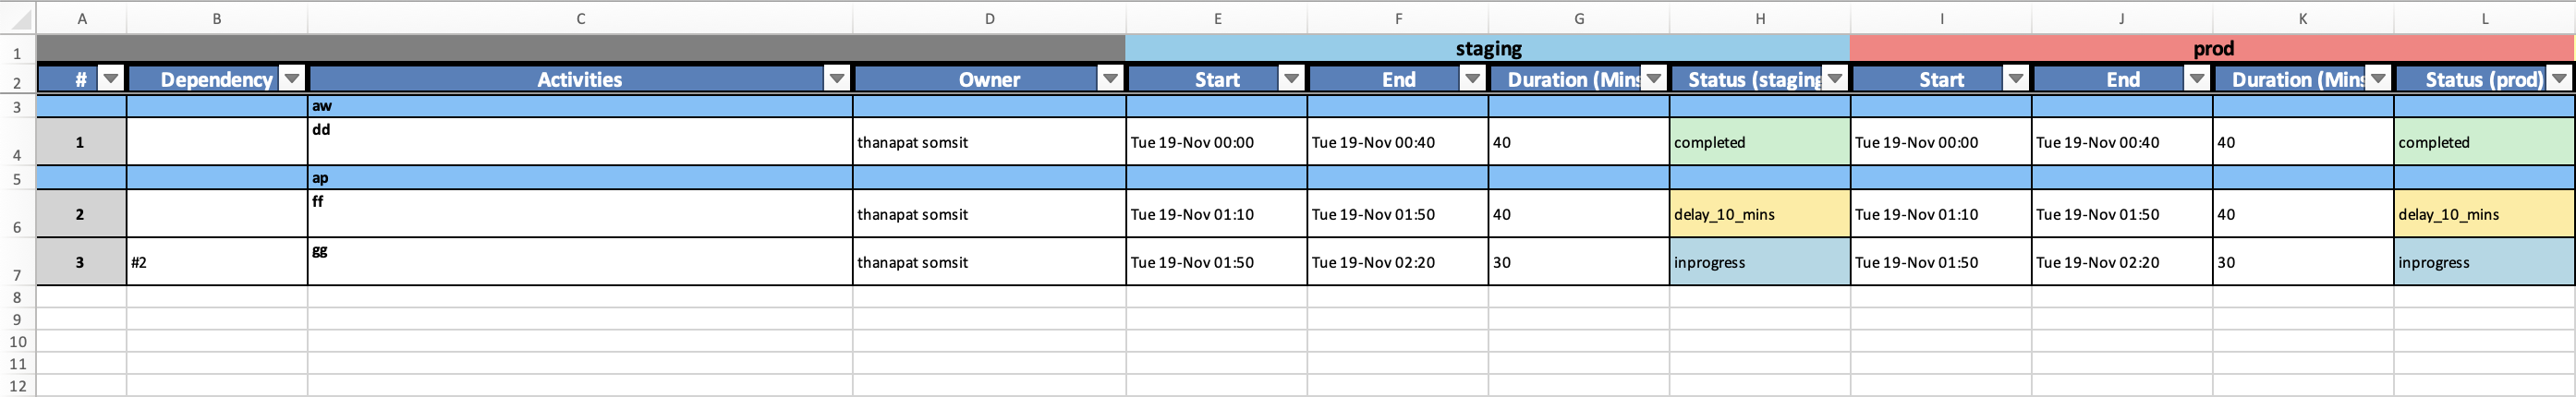
\includegraphics[width=\linewidth]{resources/pages/change-runbook/export-activity/21.png}
    \end{center}
    \caption[การส่งออกไฟล์ Excel]{การส่งออกไฟล์ Excel}
  \label{fig:excel-export}
\end{figure}

\newpage
\section{การใช้งานฟีเจอร์ Custom Library}
\subsection{การสร้าง Custom Library Repostory}
\begin{center}
    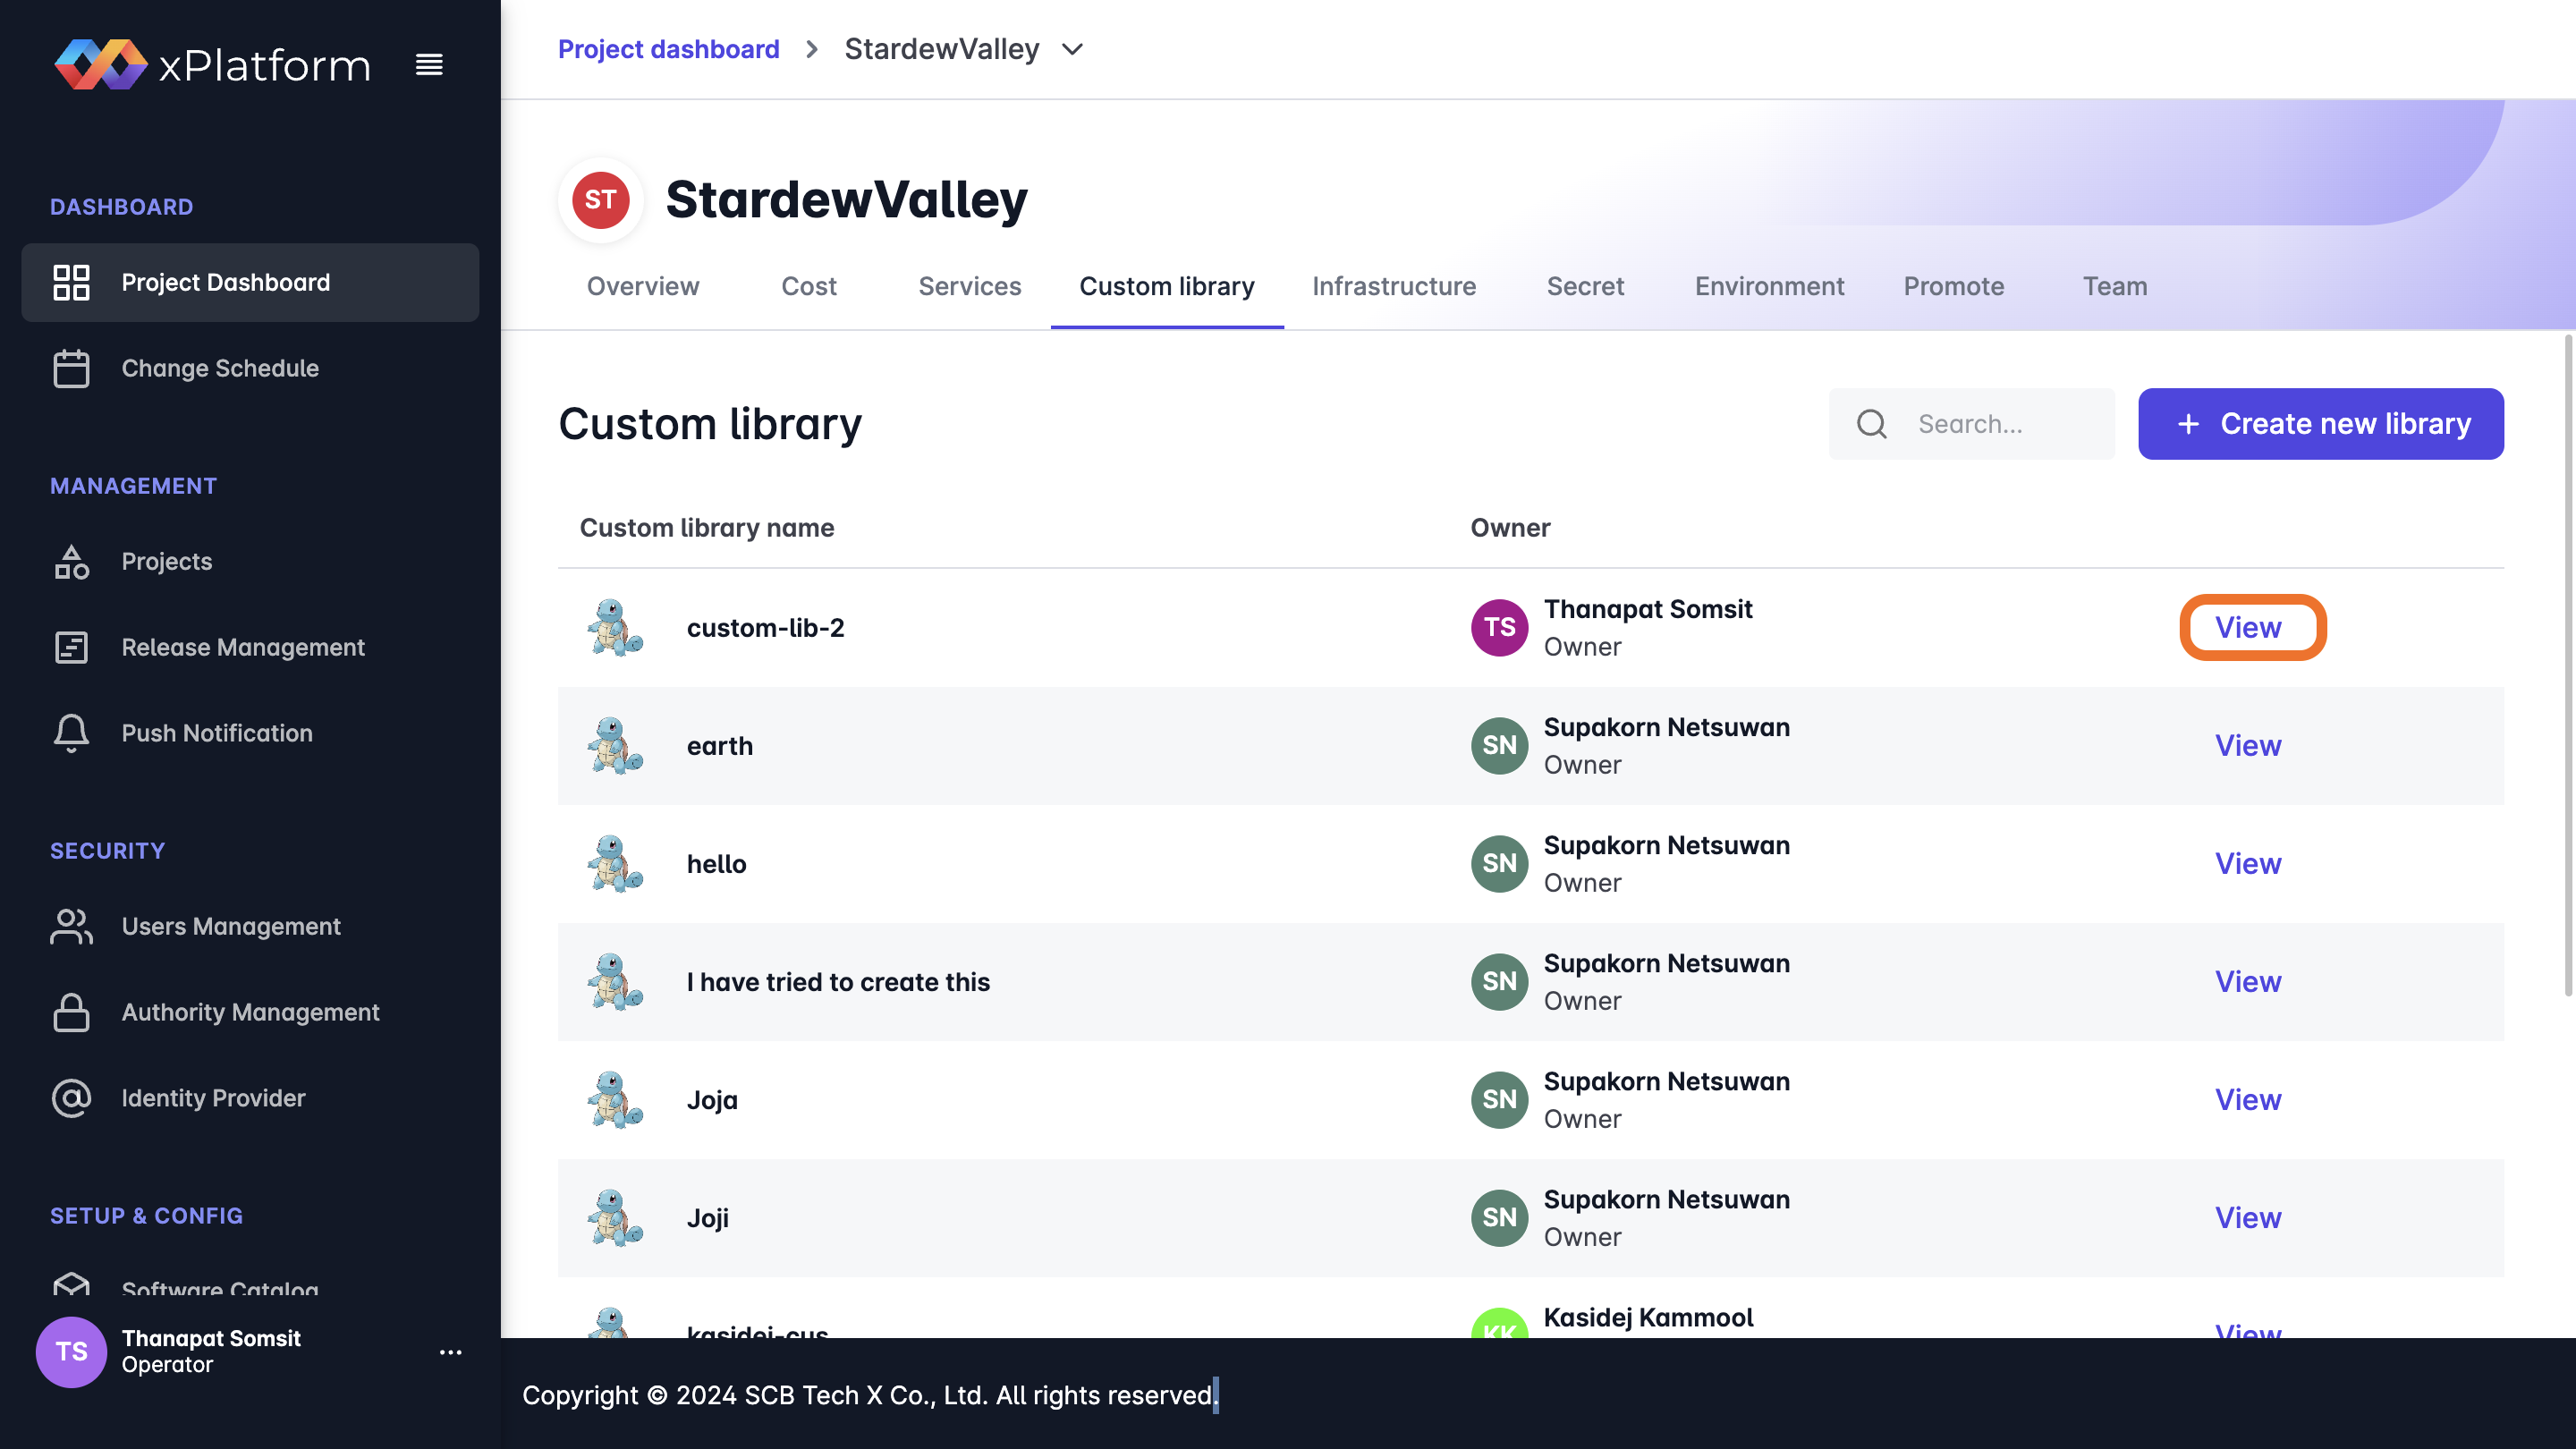
\includegraphics[width=\linewidth]{resources/pages/custom-library/create-library/1.png}

    \vspace{1in}

    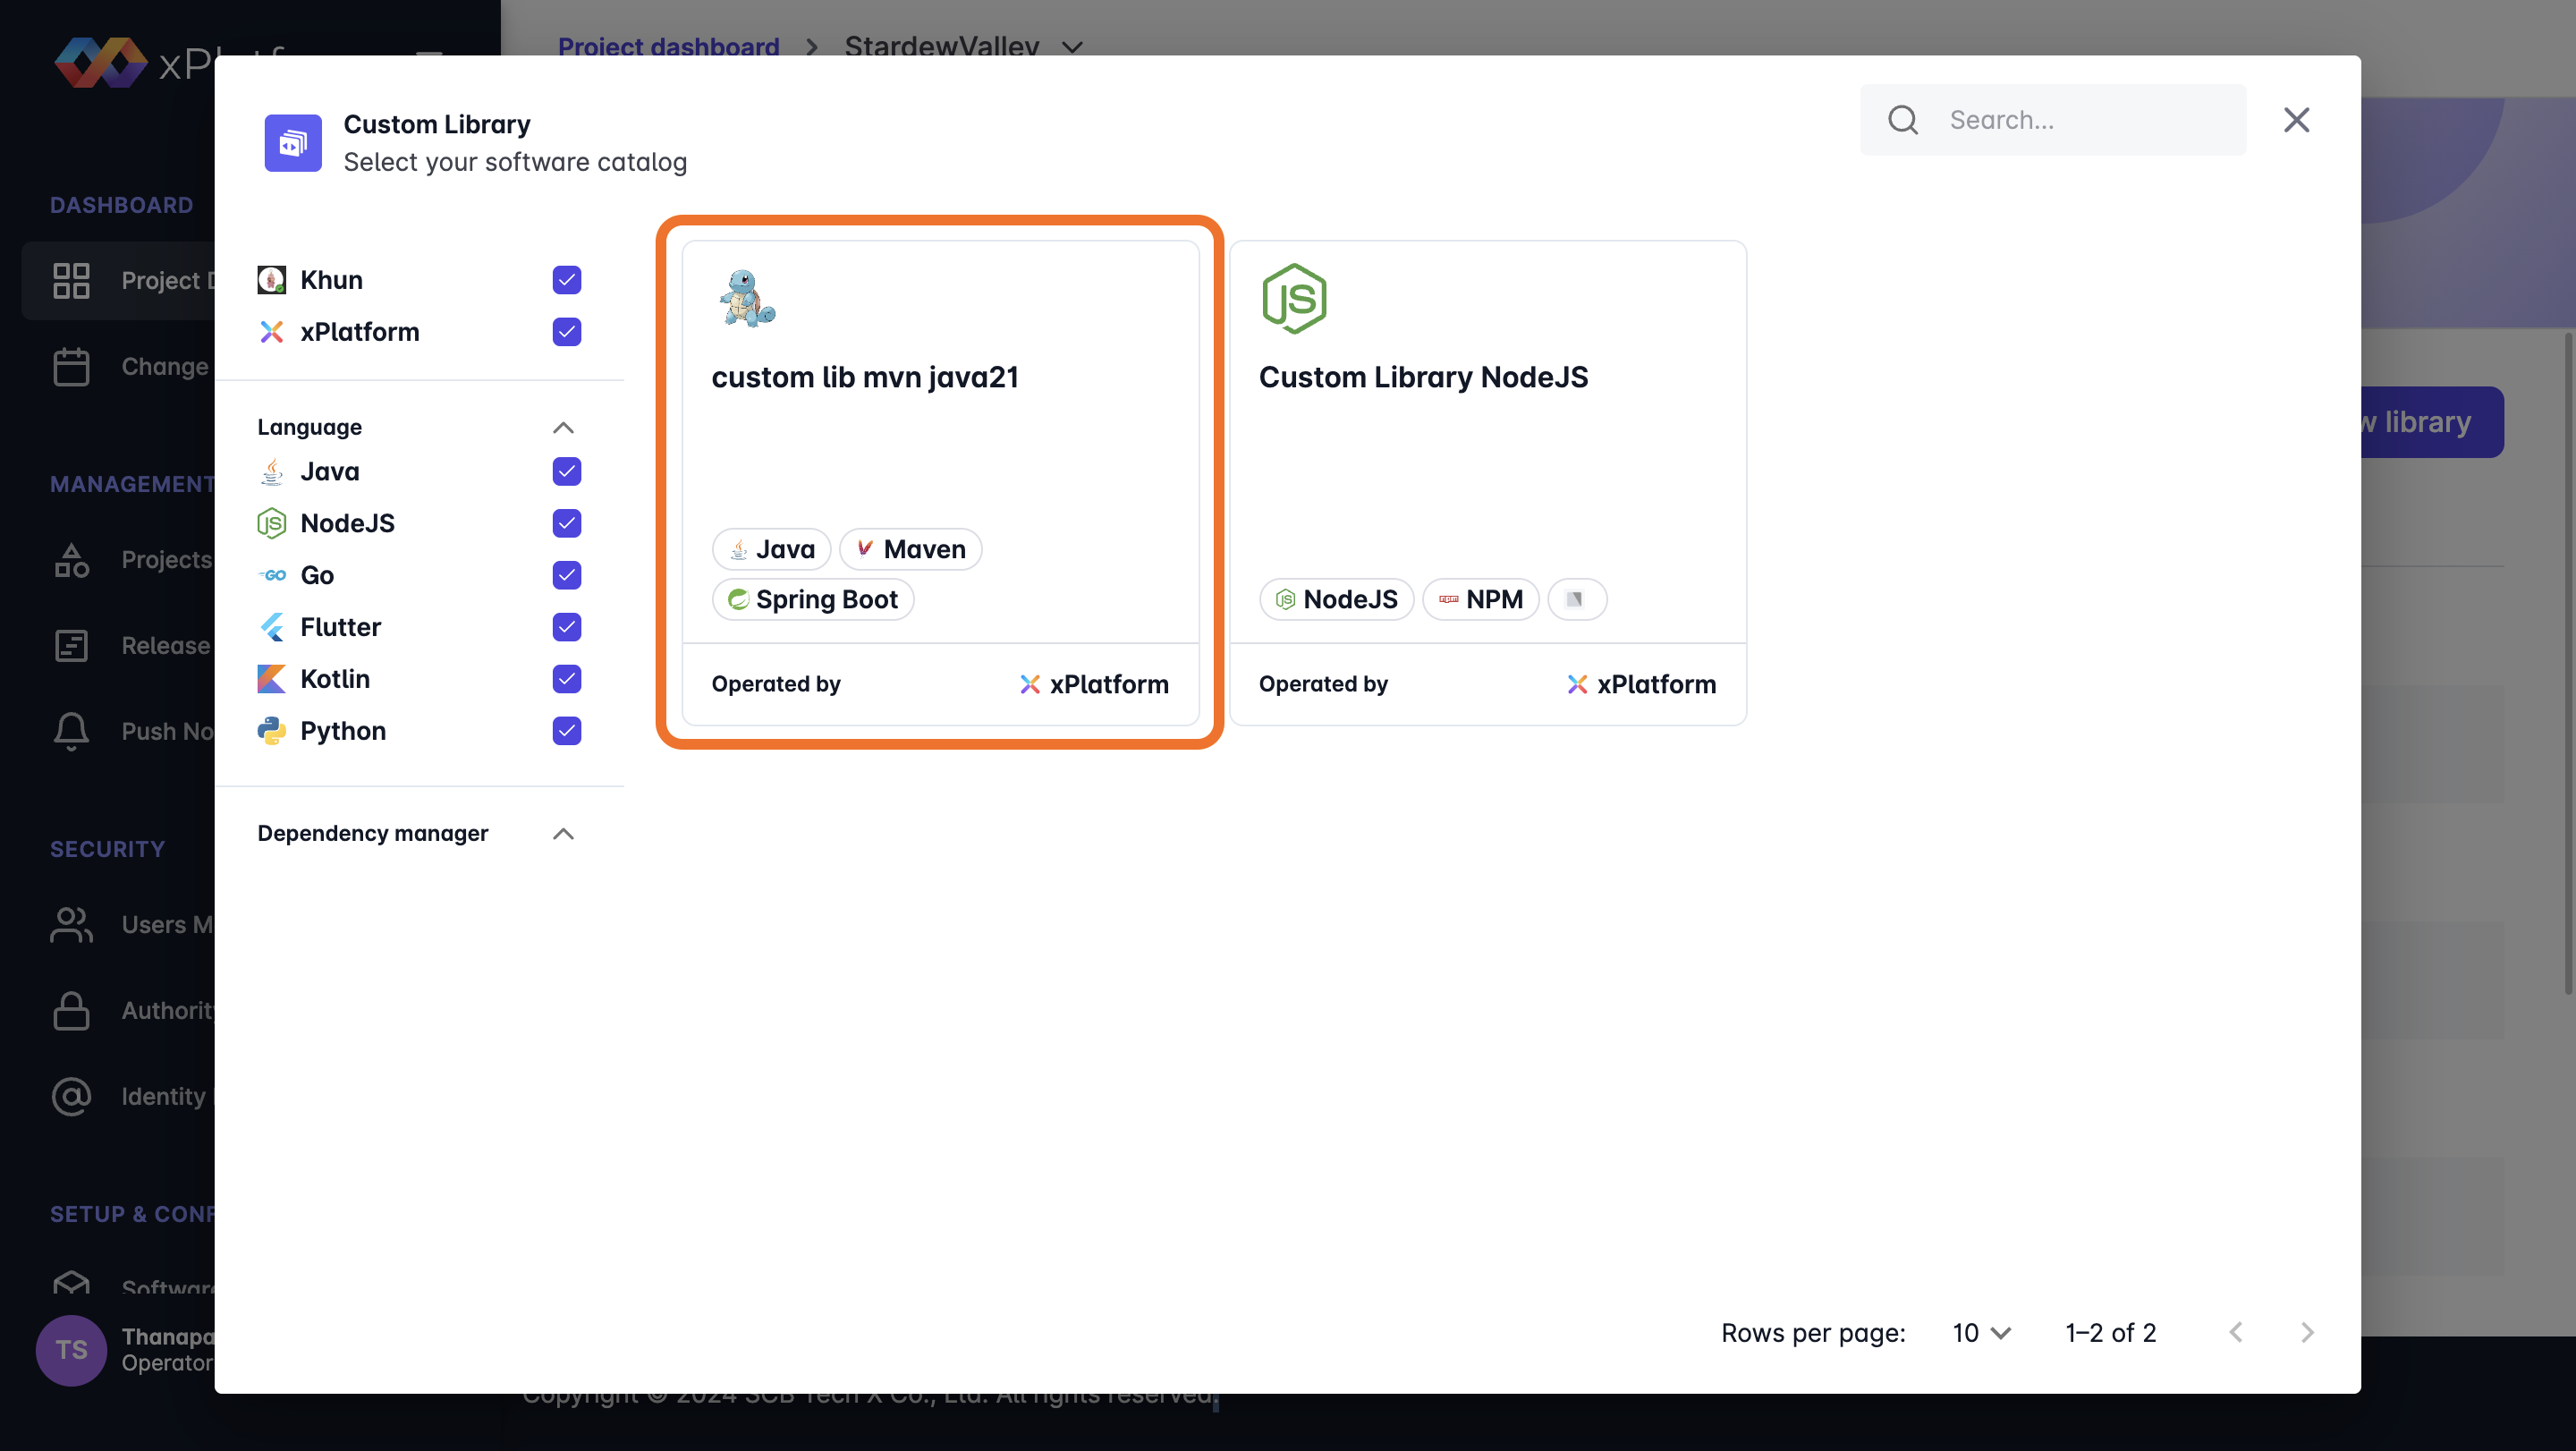
\includegraphics[width=\linewidth]{resources/pages/custom-library/create-library/2.png}
\end{center}
\begin{center}
    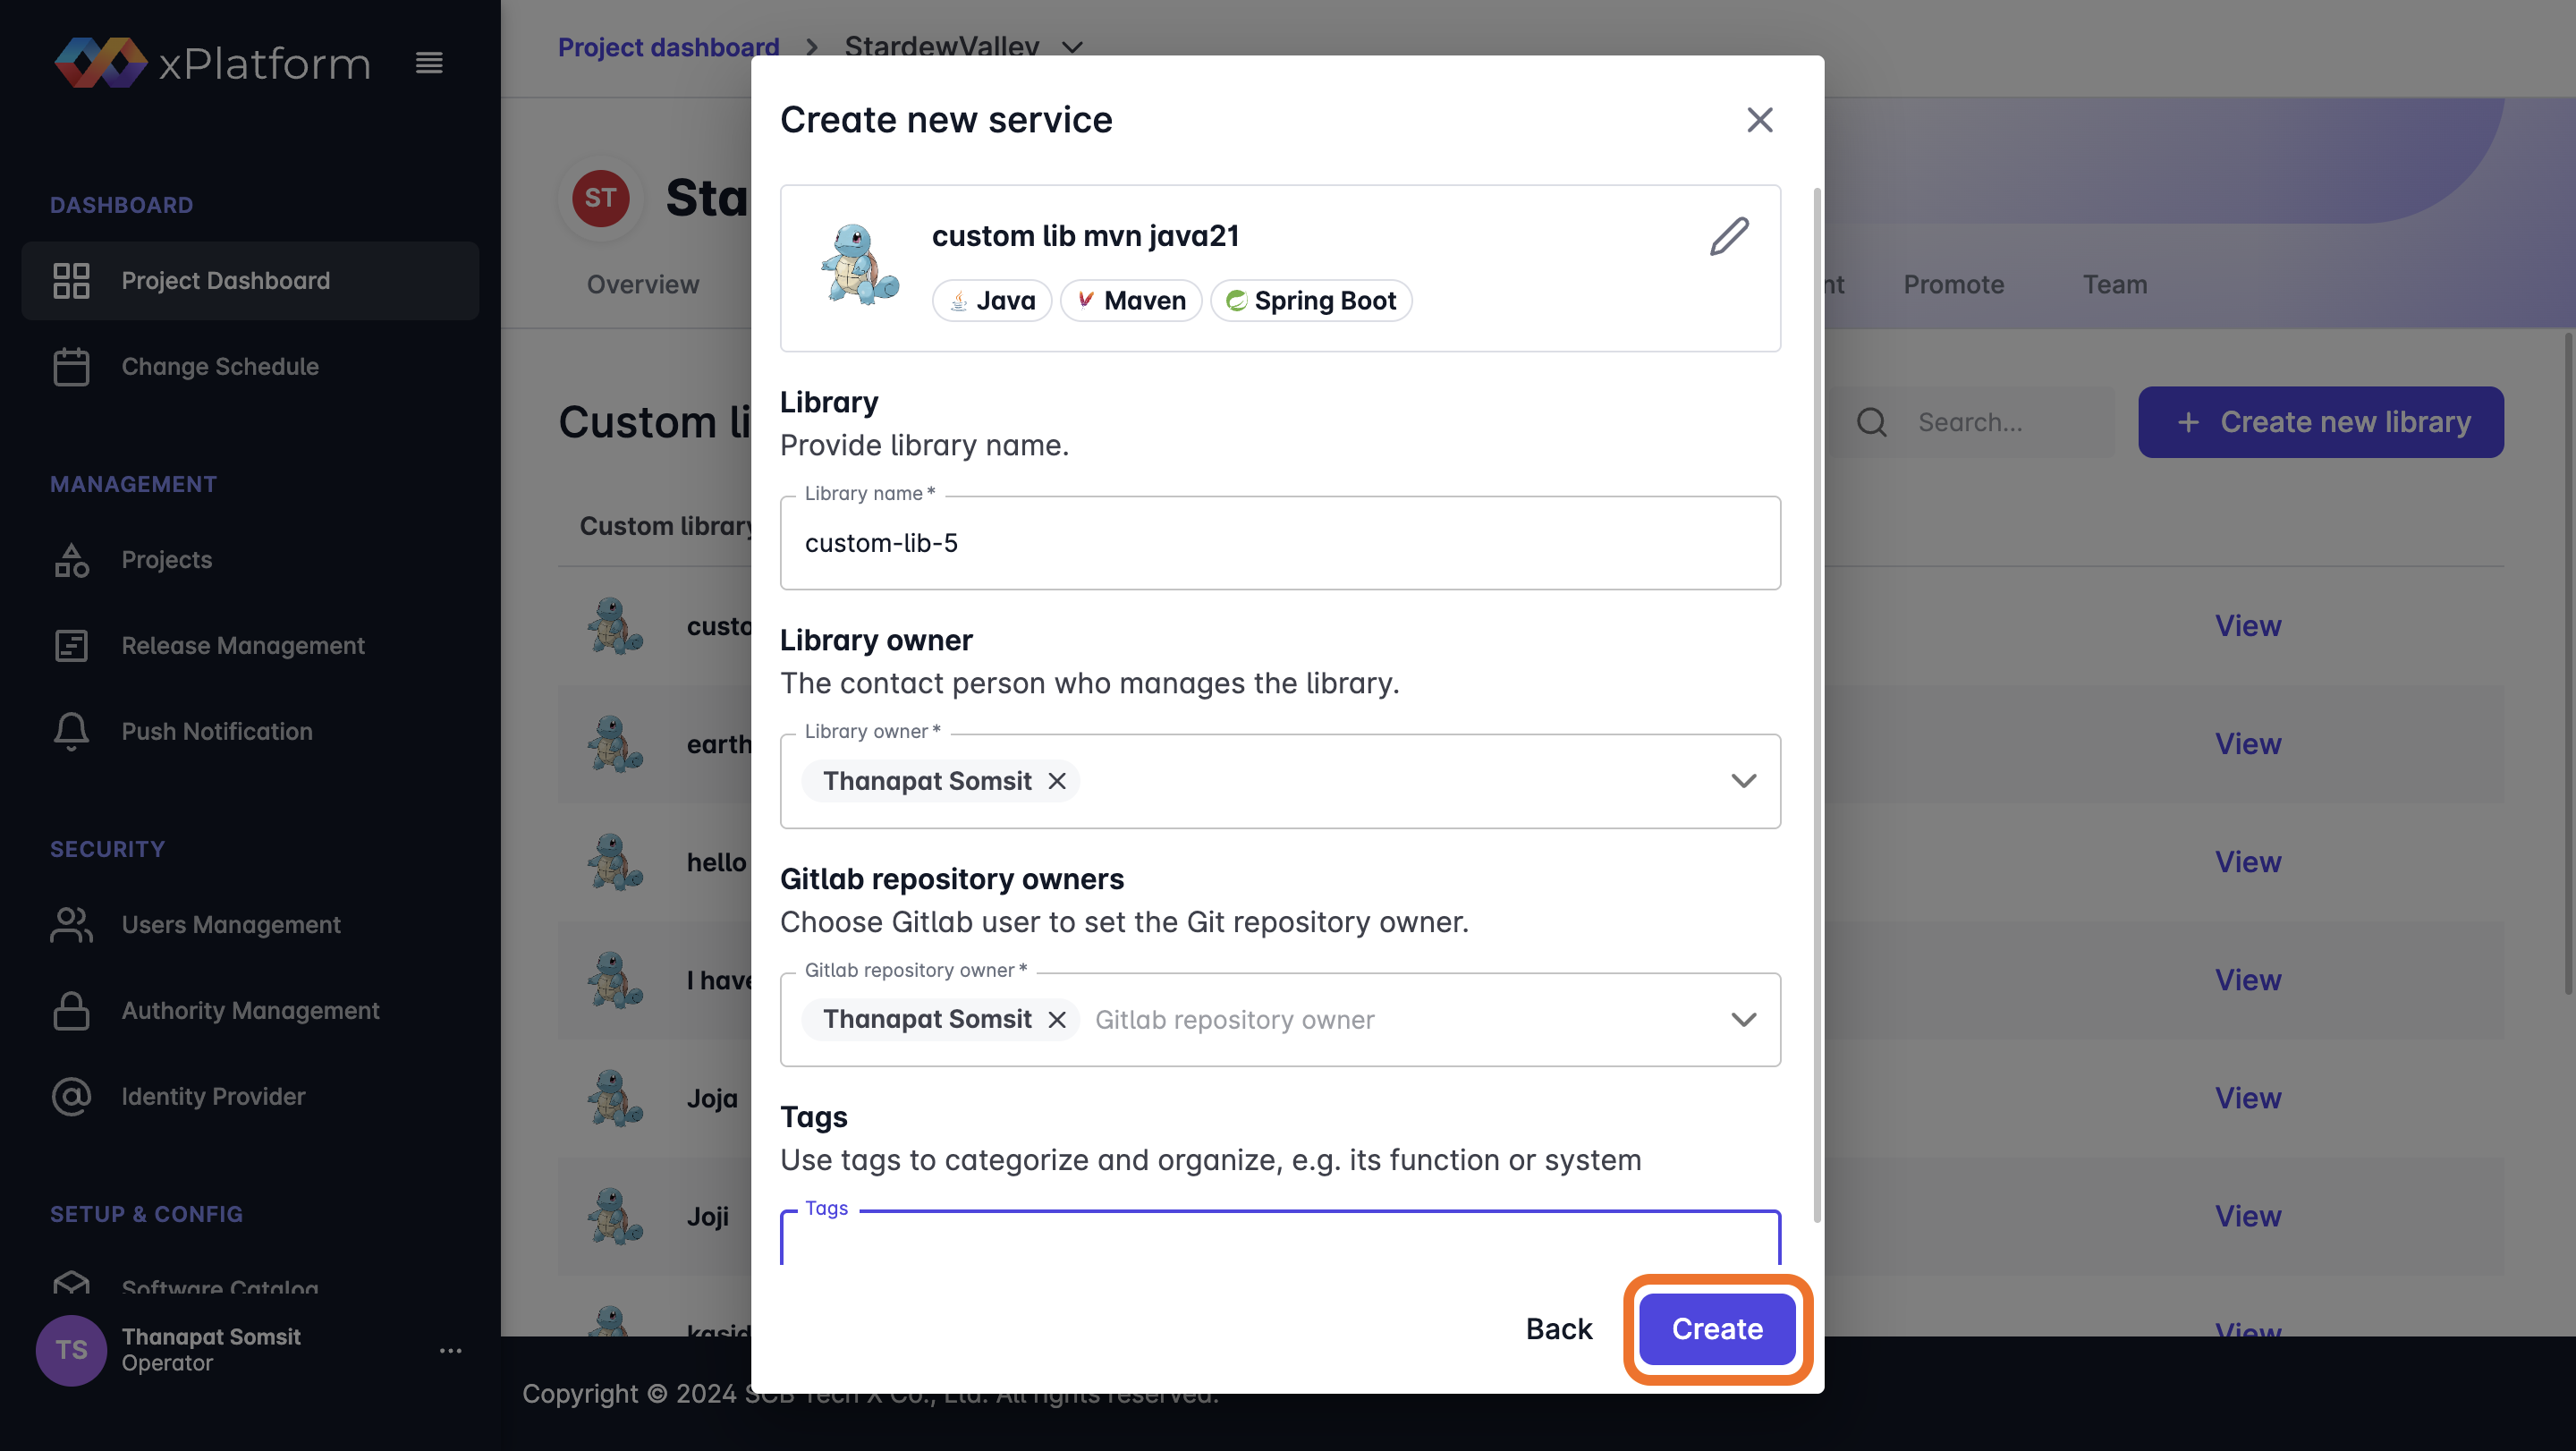
\includegraphics[width=\linewidth]{resources/pages/custom-library/create-library/3.png}

    \vspace{1in}

    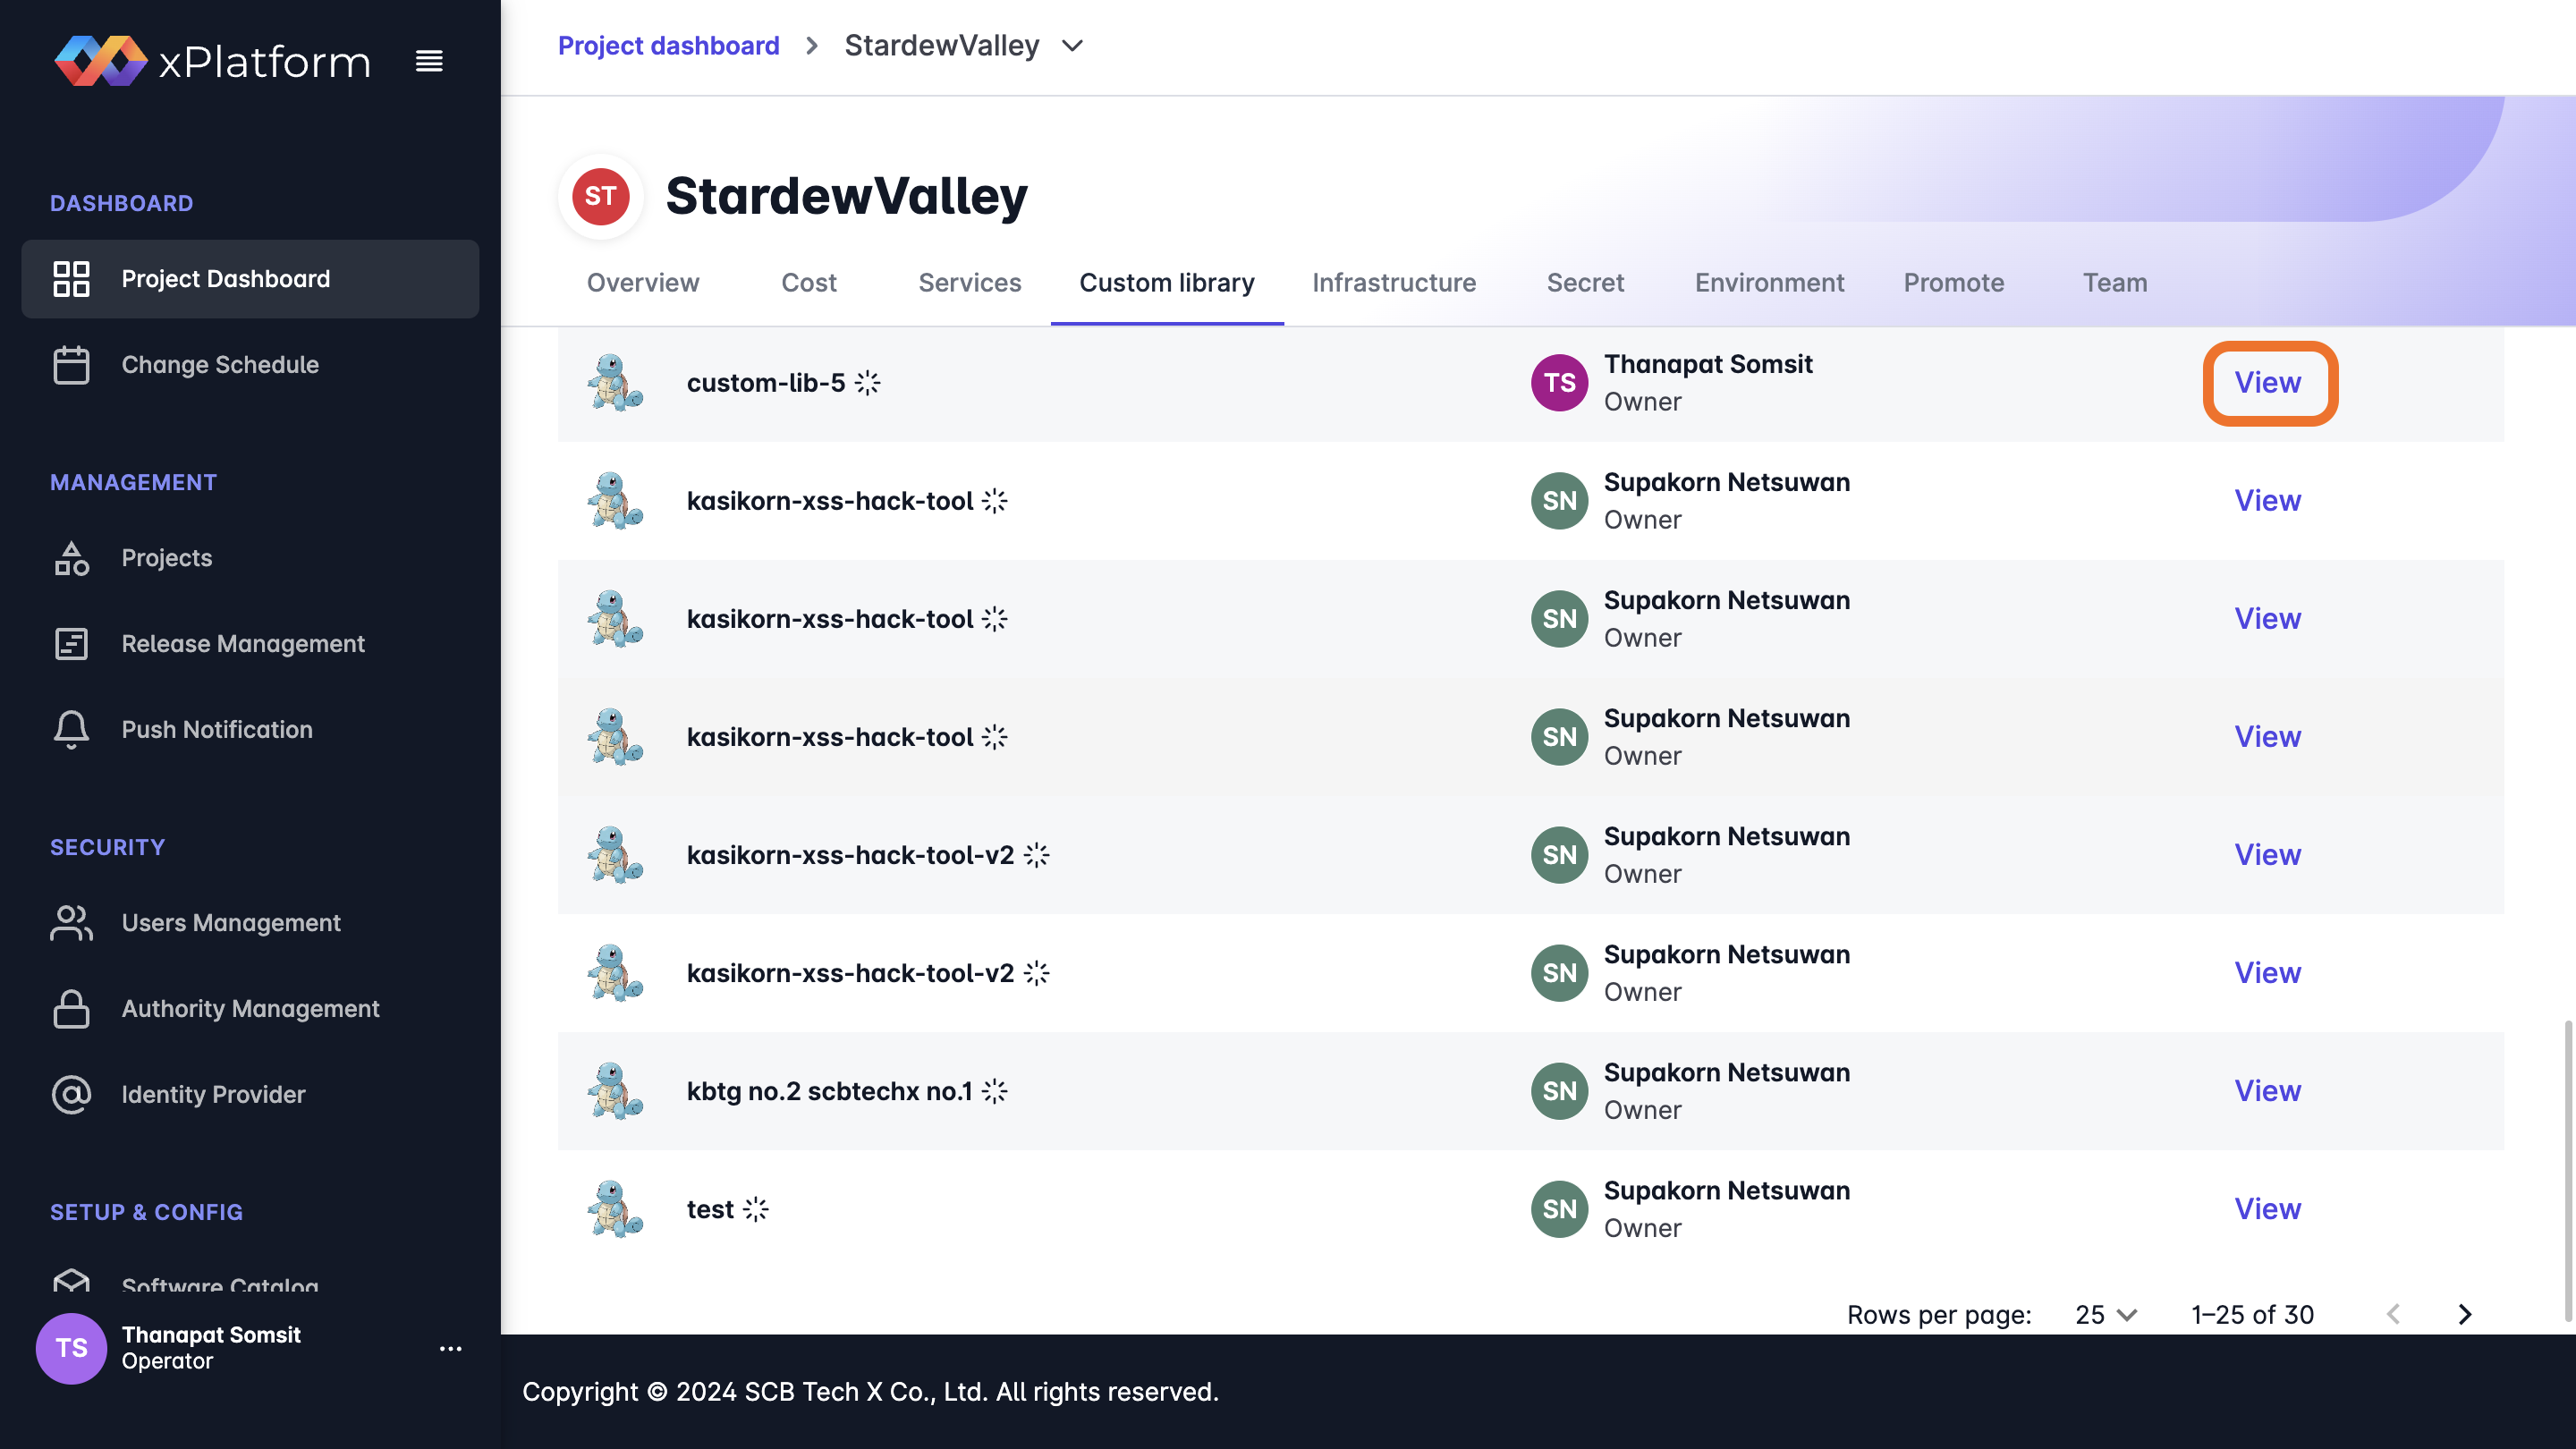
\includegraphics[width=\linewidth]{resources/pages/custom-library/create-library/4.png}
\end{center}

\begin{figure}[H]
    \begin{center}
        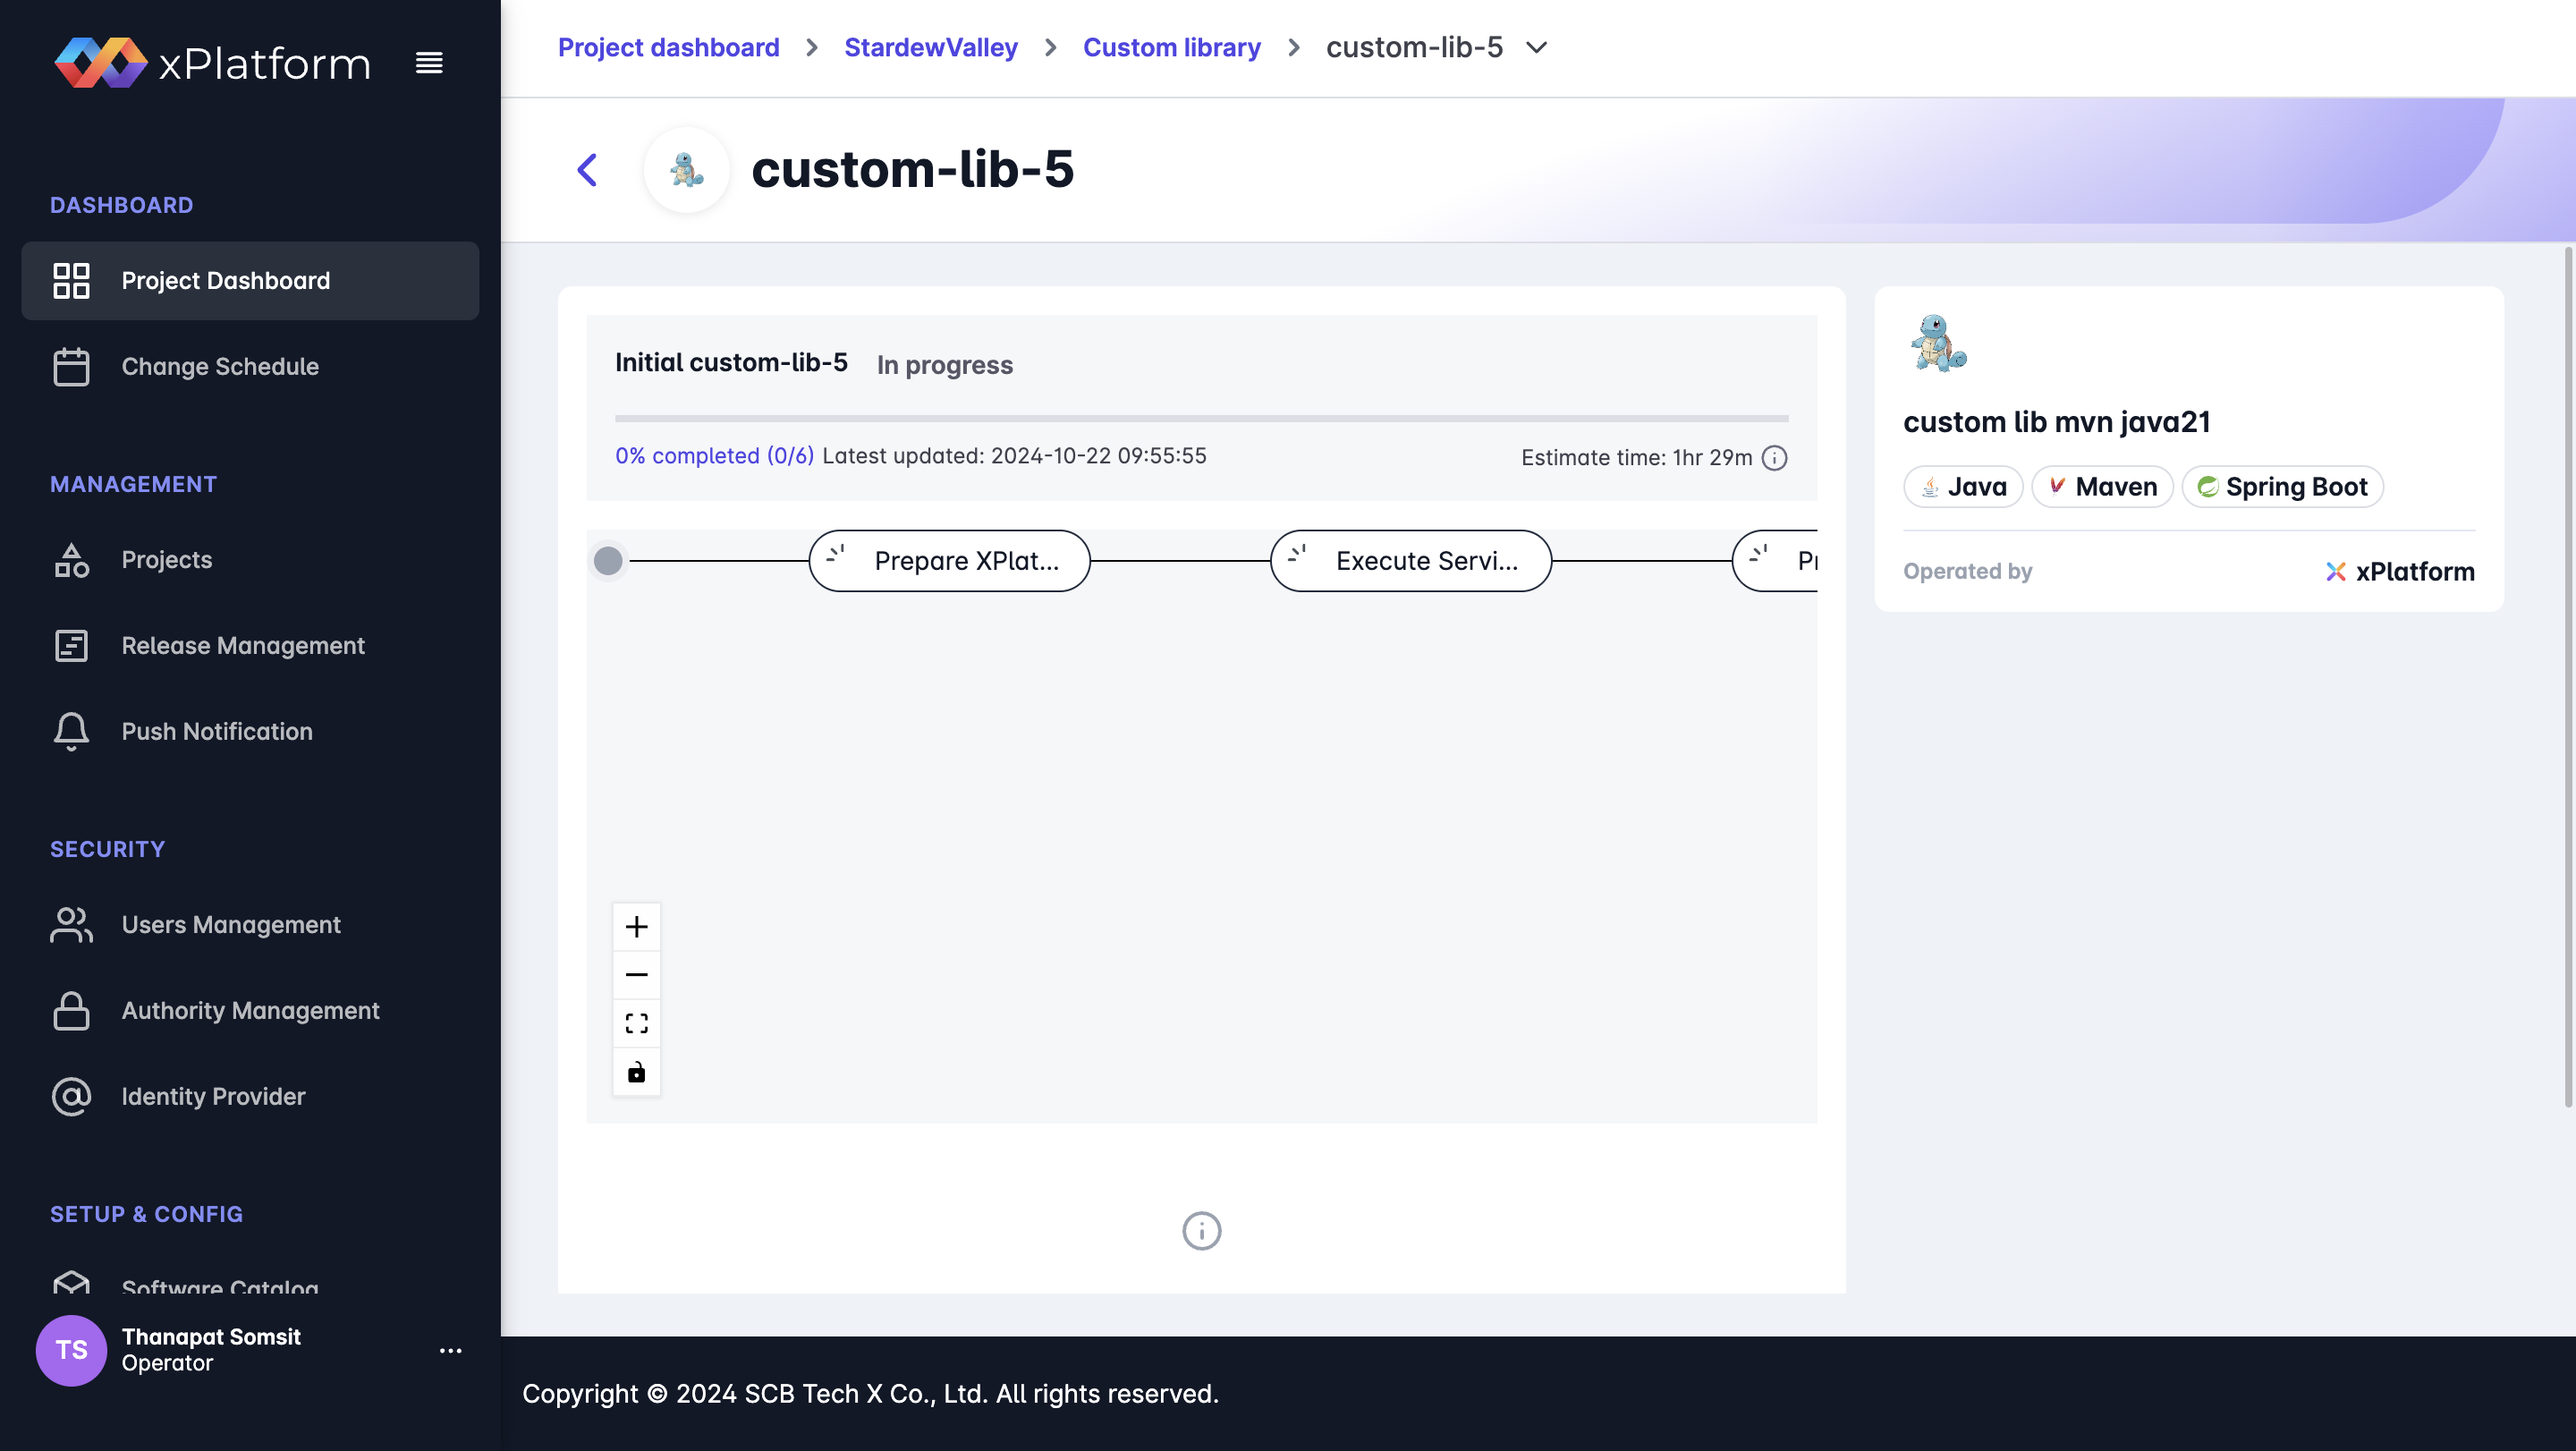
\includegraphics[width=\linewidth]{resources/pages/custom-library/create-library/5.png}
    
        \vspace{1in}
    
        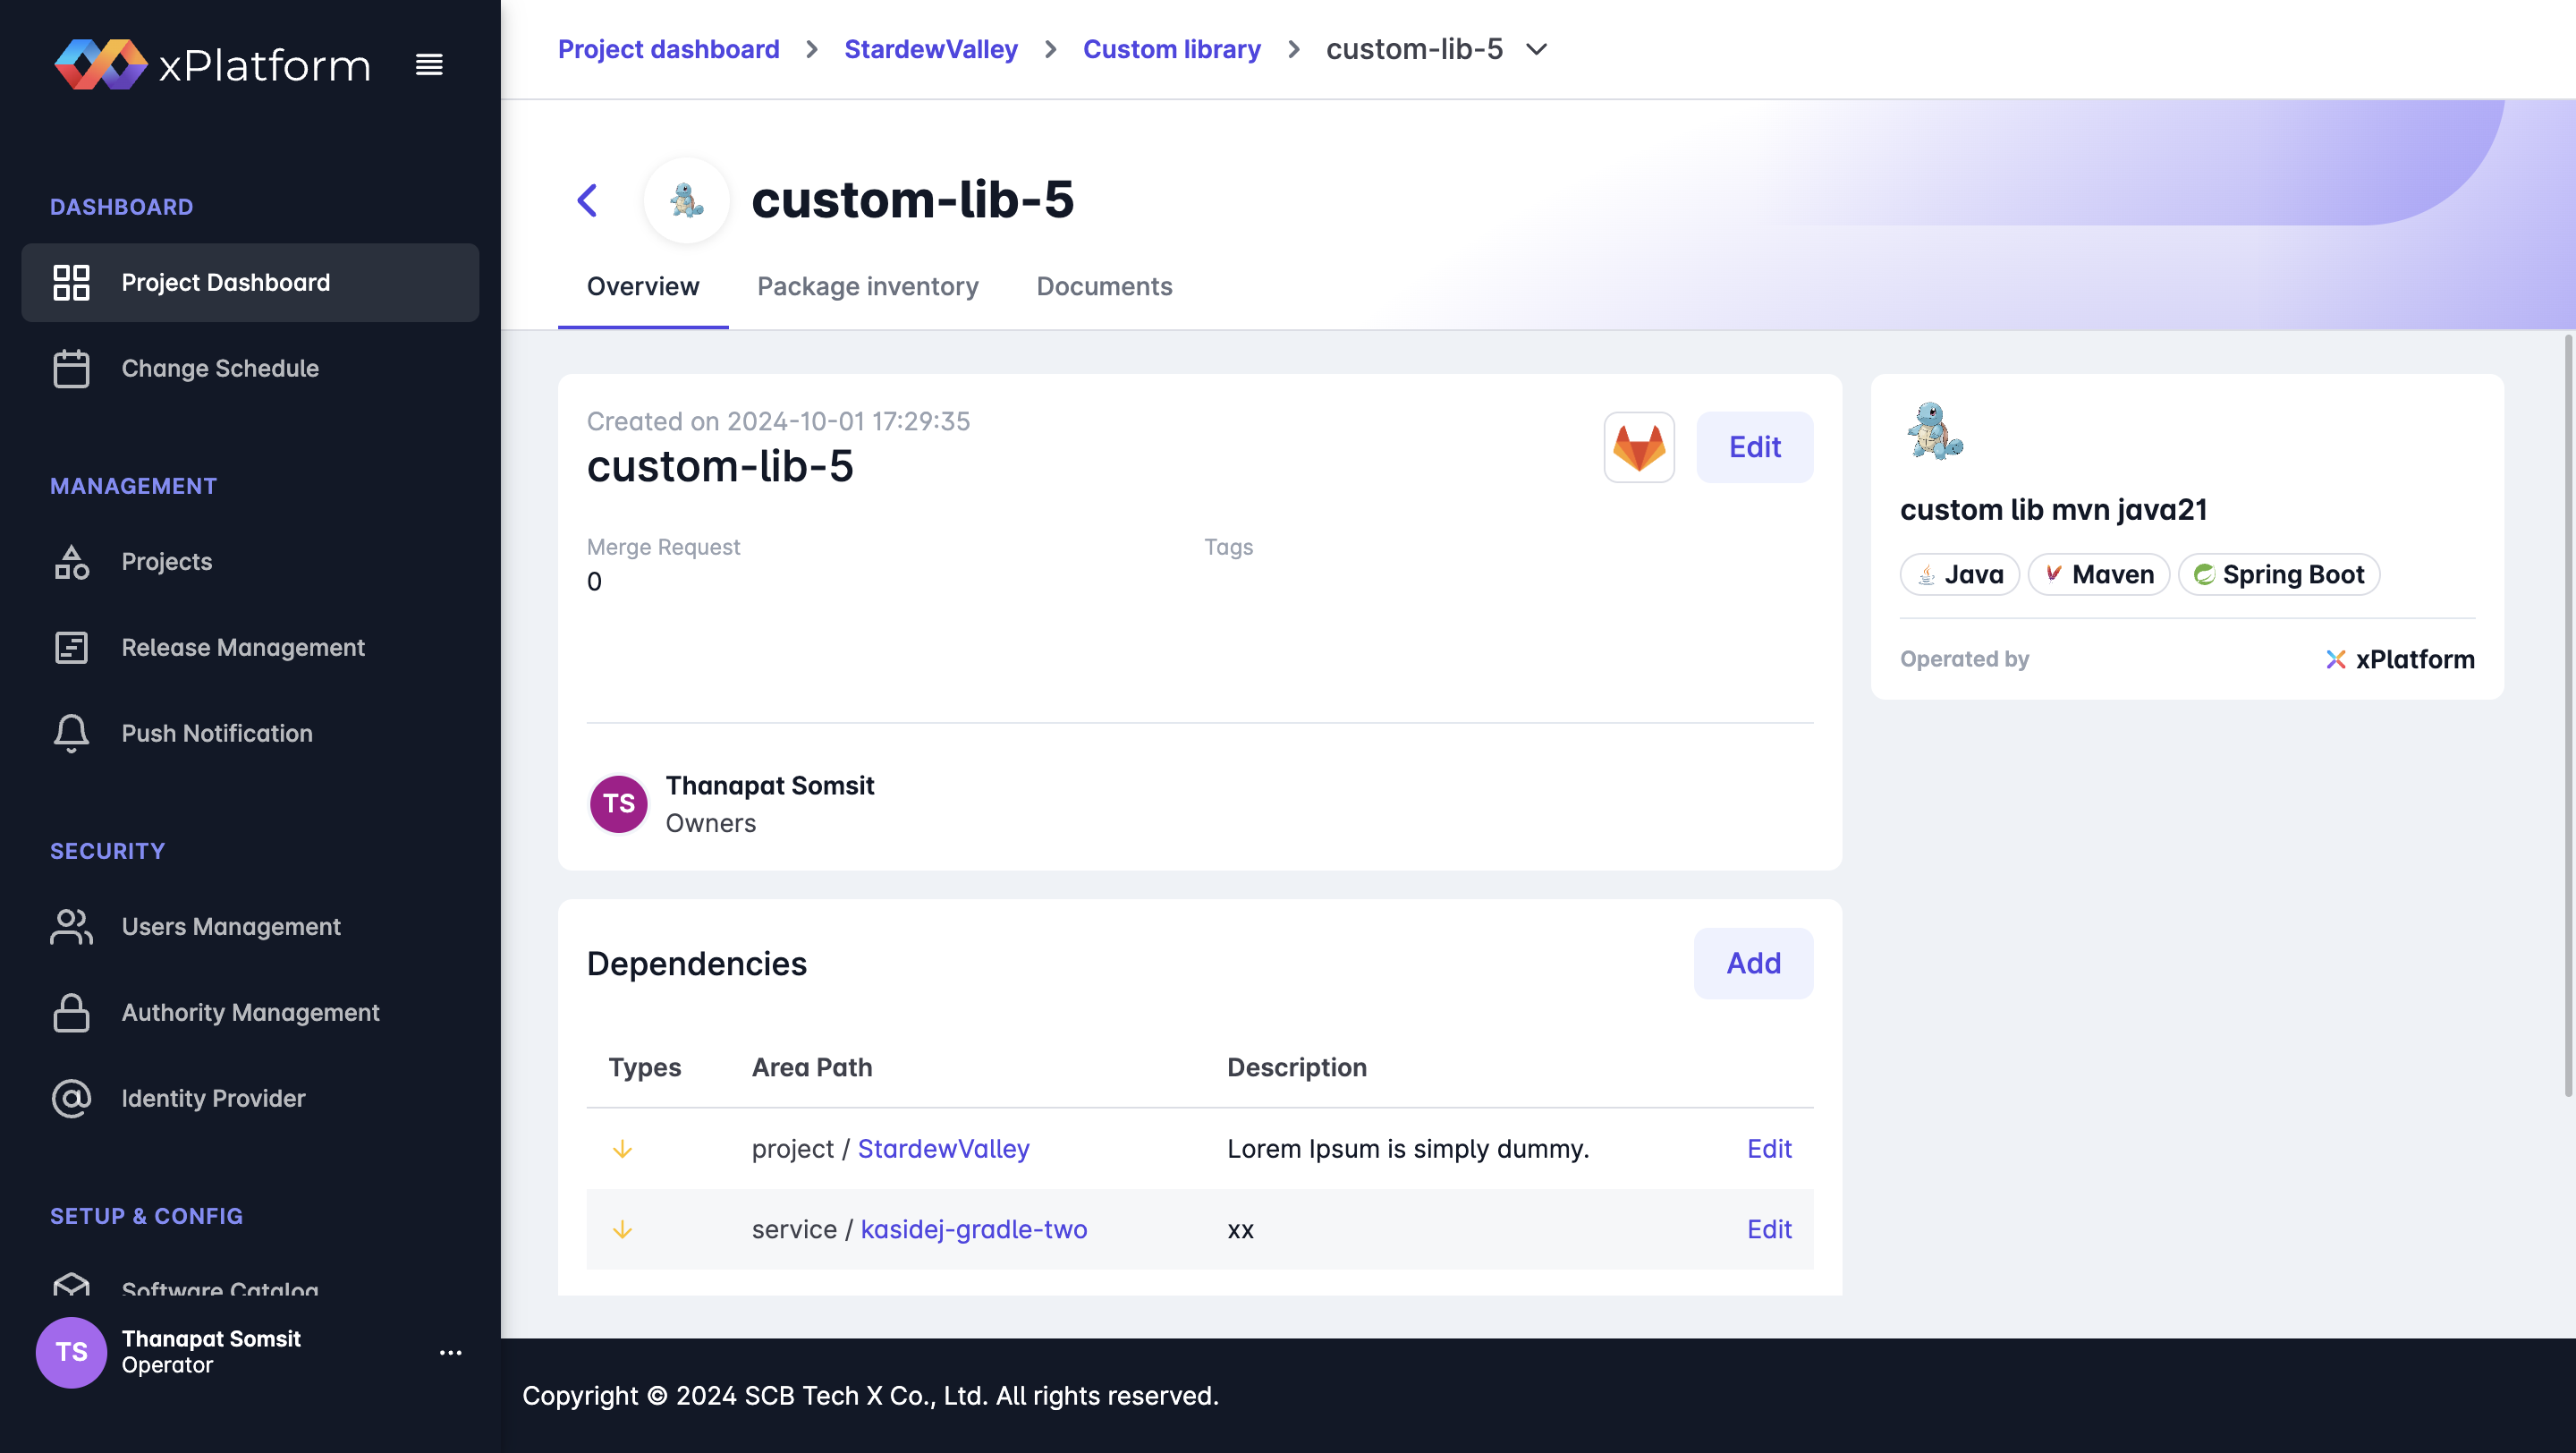
\includegraphics[width=\linewidth]{resources/pages/custom-library/create-library/6.png}
    \end{center}
    \caption[การสร้าง Custom Library]{การสร้าง Custom Library}
  \label{fig:create-library}
\end{figure}

\newpage
\subsection{การอัพเดตเวอร์ชัน Custom Library}
\begin{center}
    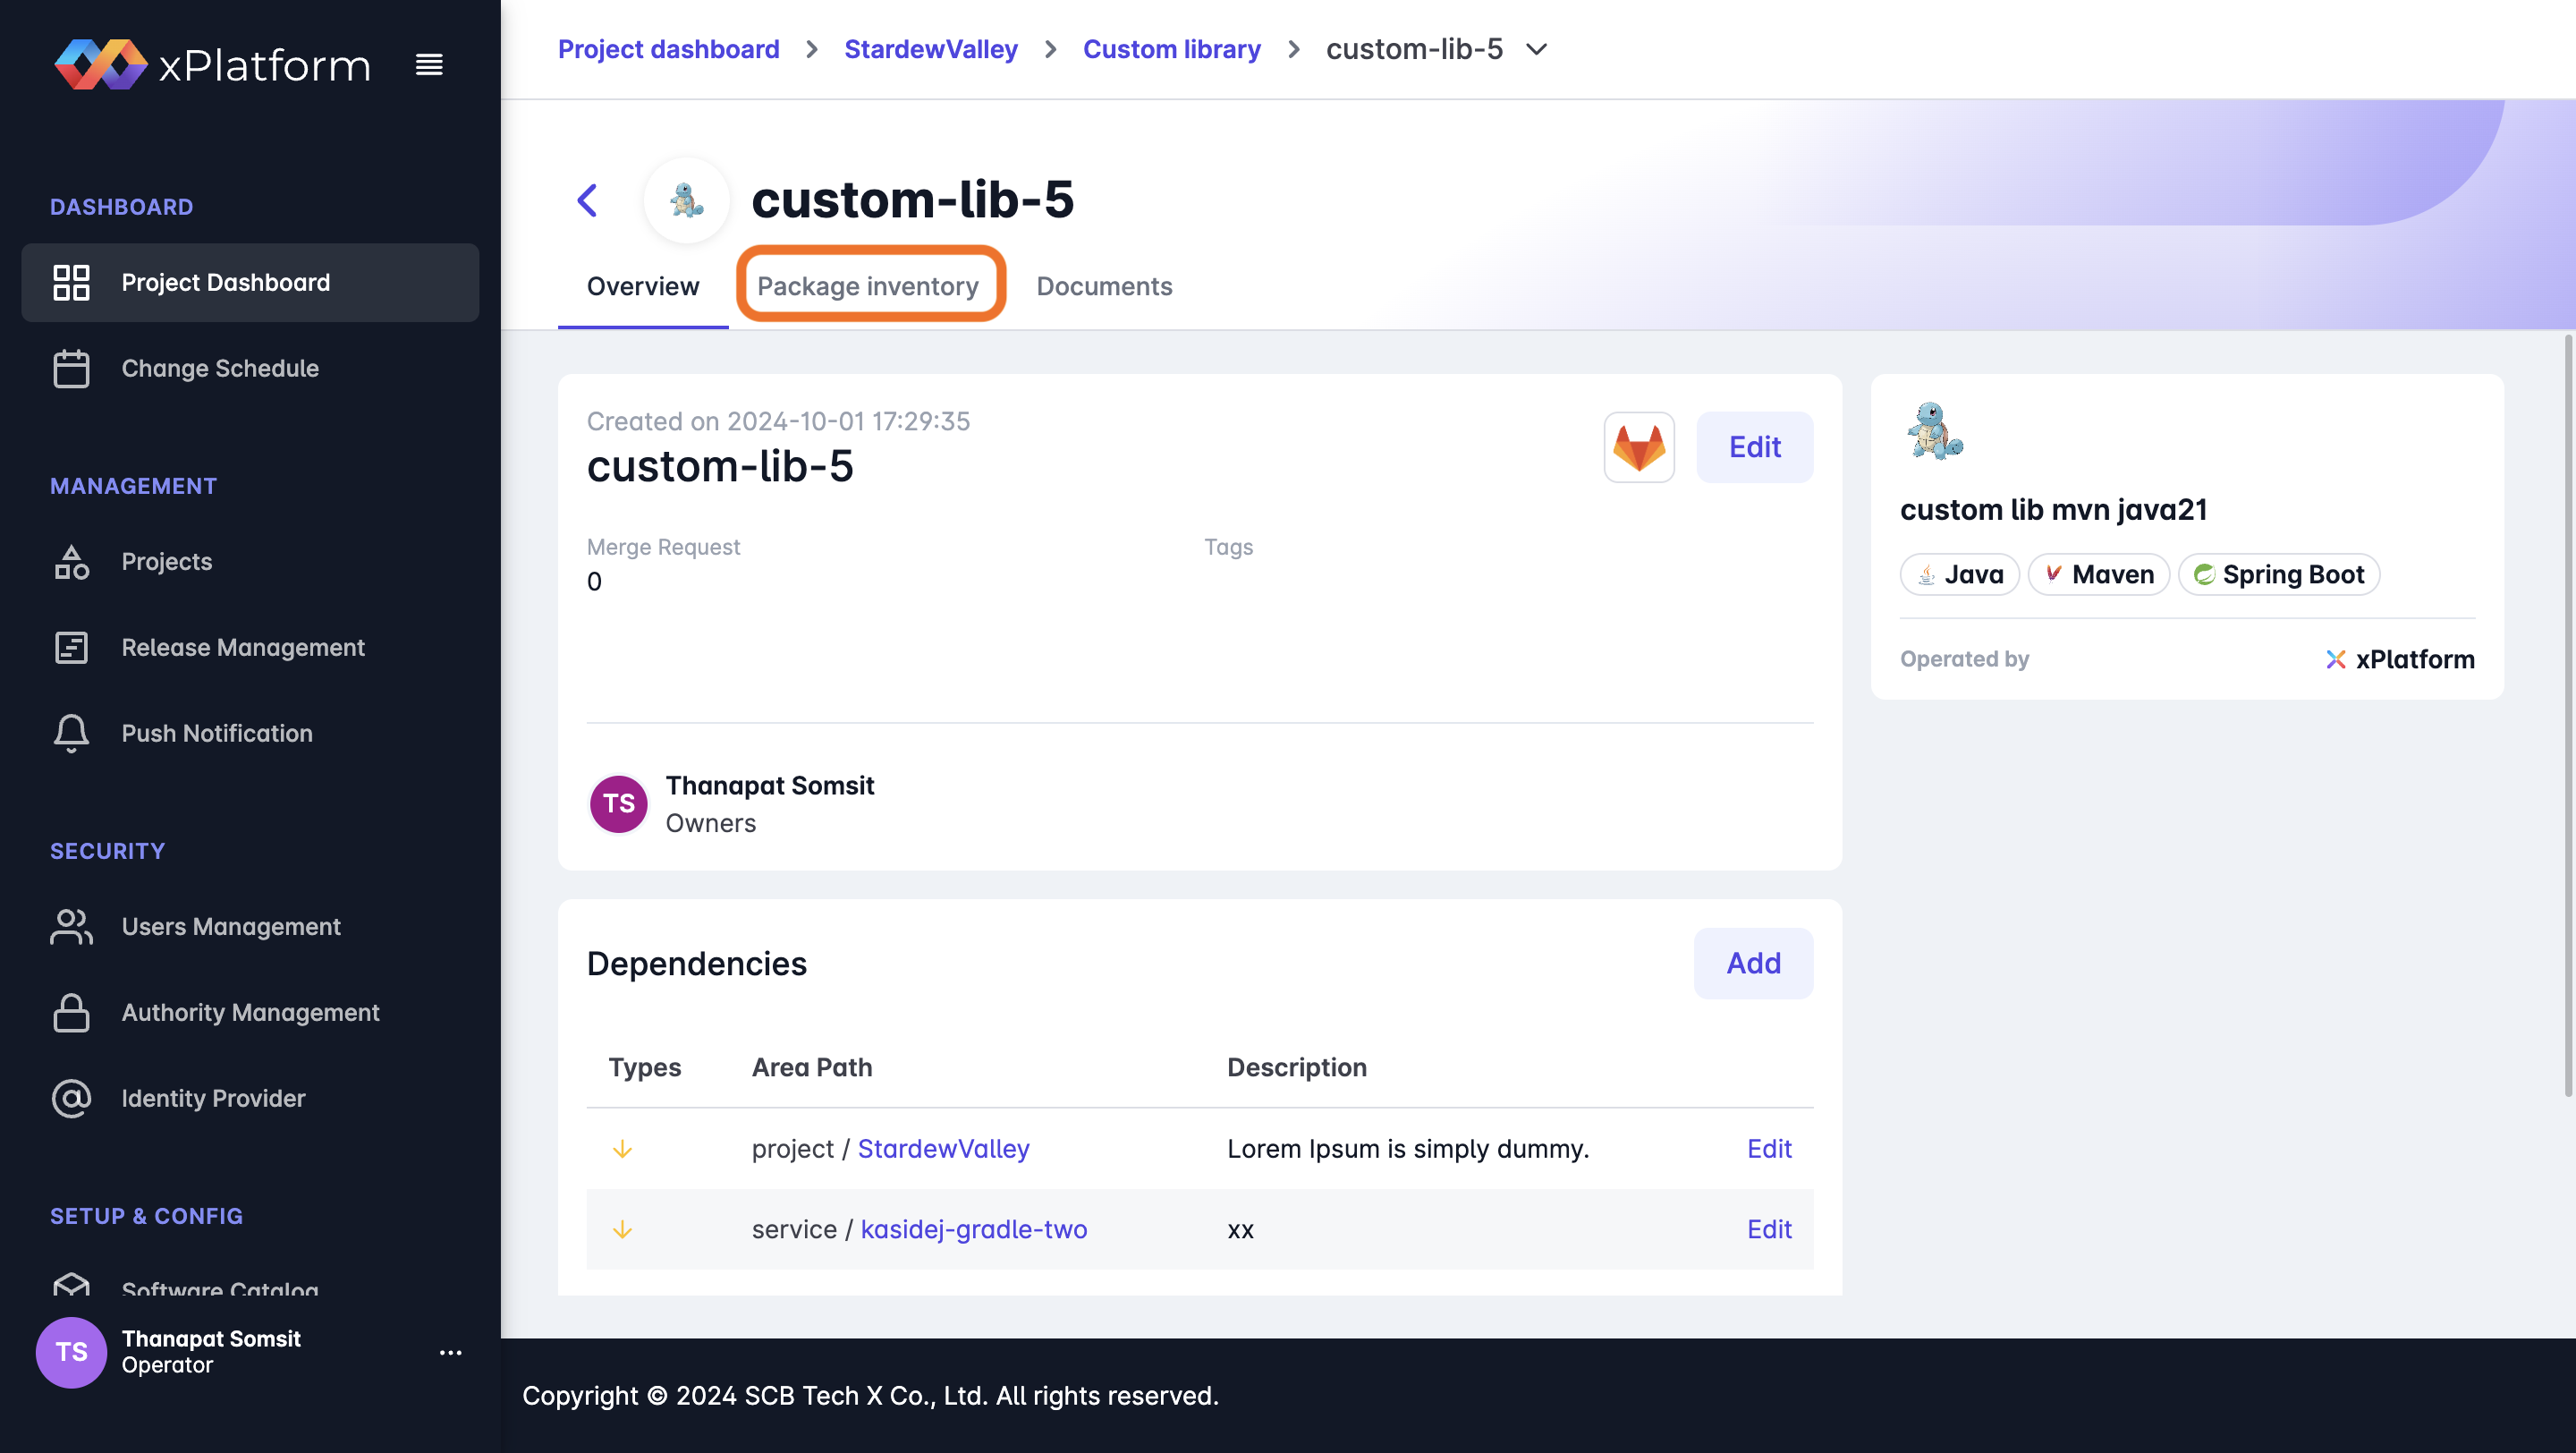
\includegraphics[width=\linewidth]{resources/pages/custom-library/update-library/6.png}

    \vspace{1in}

    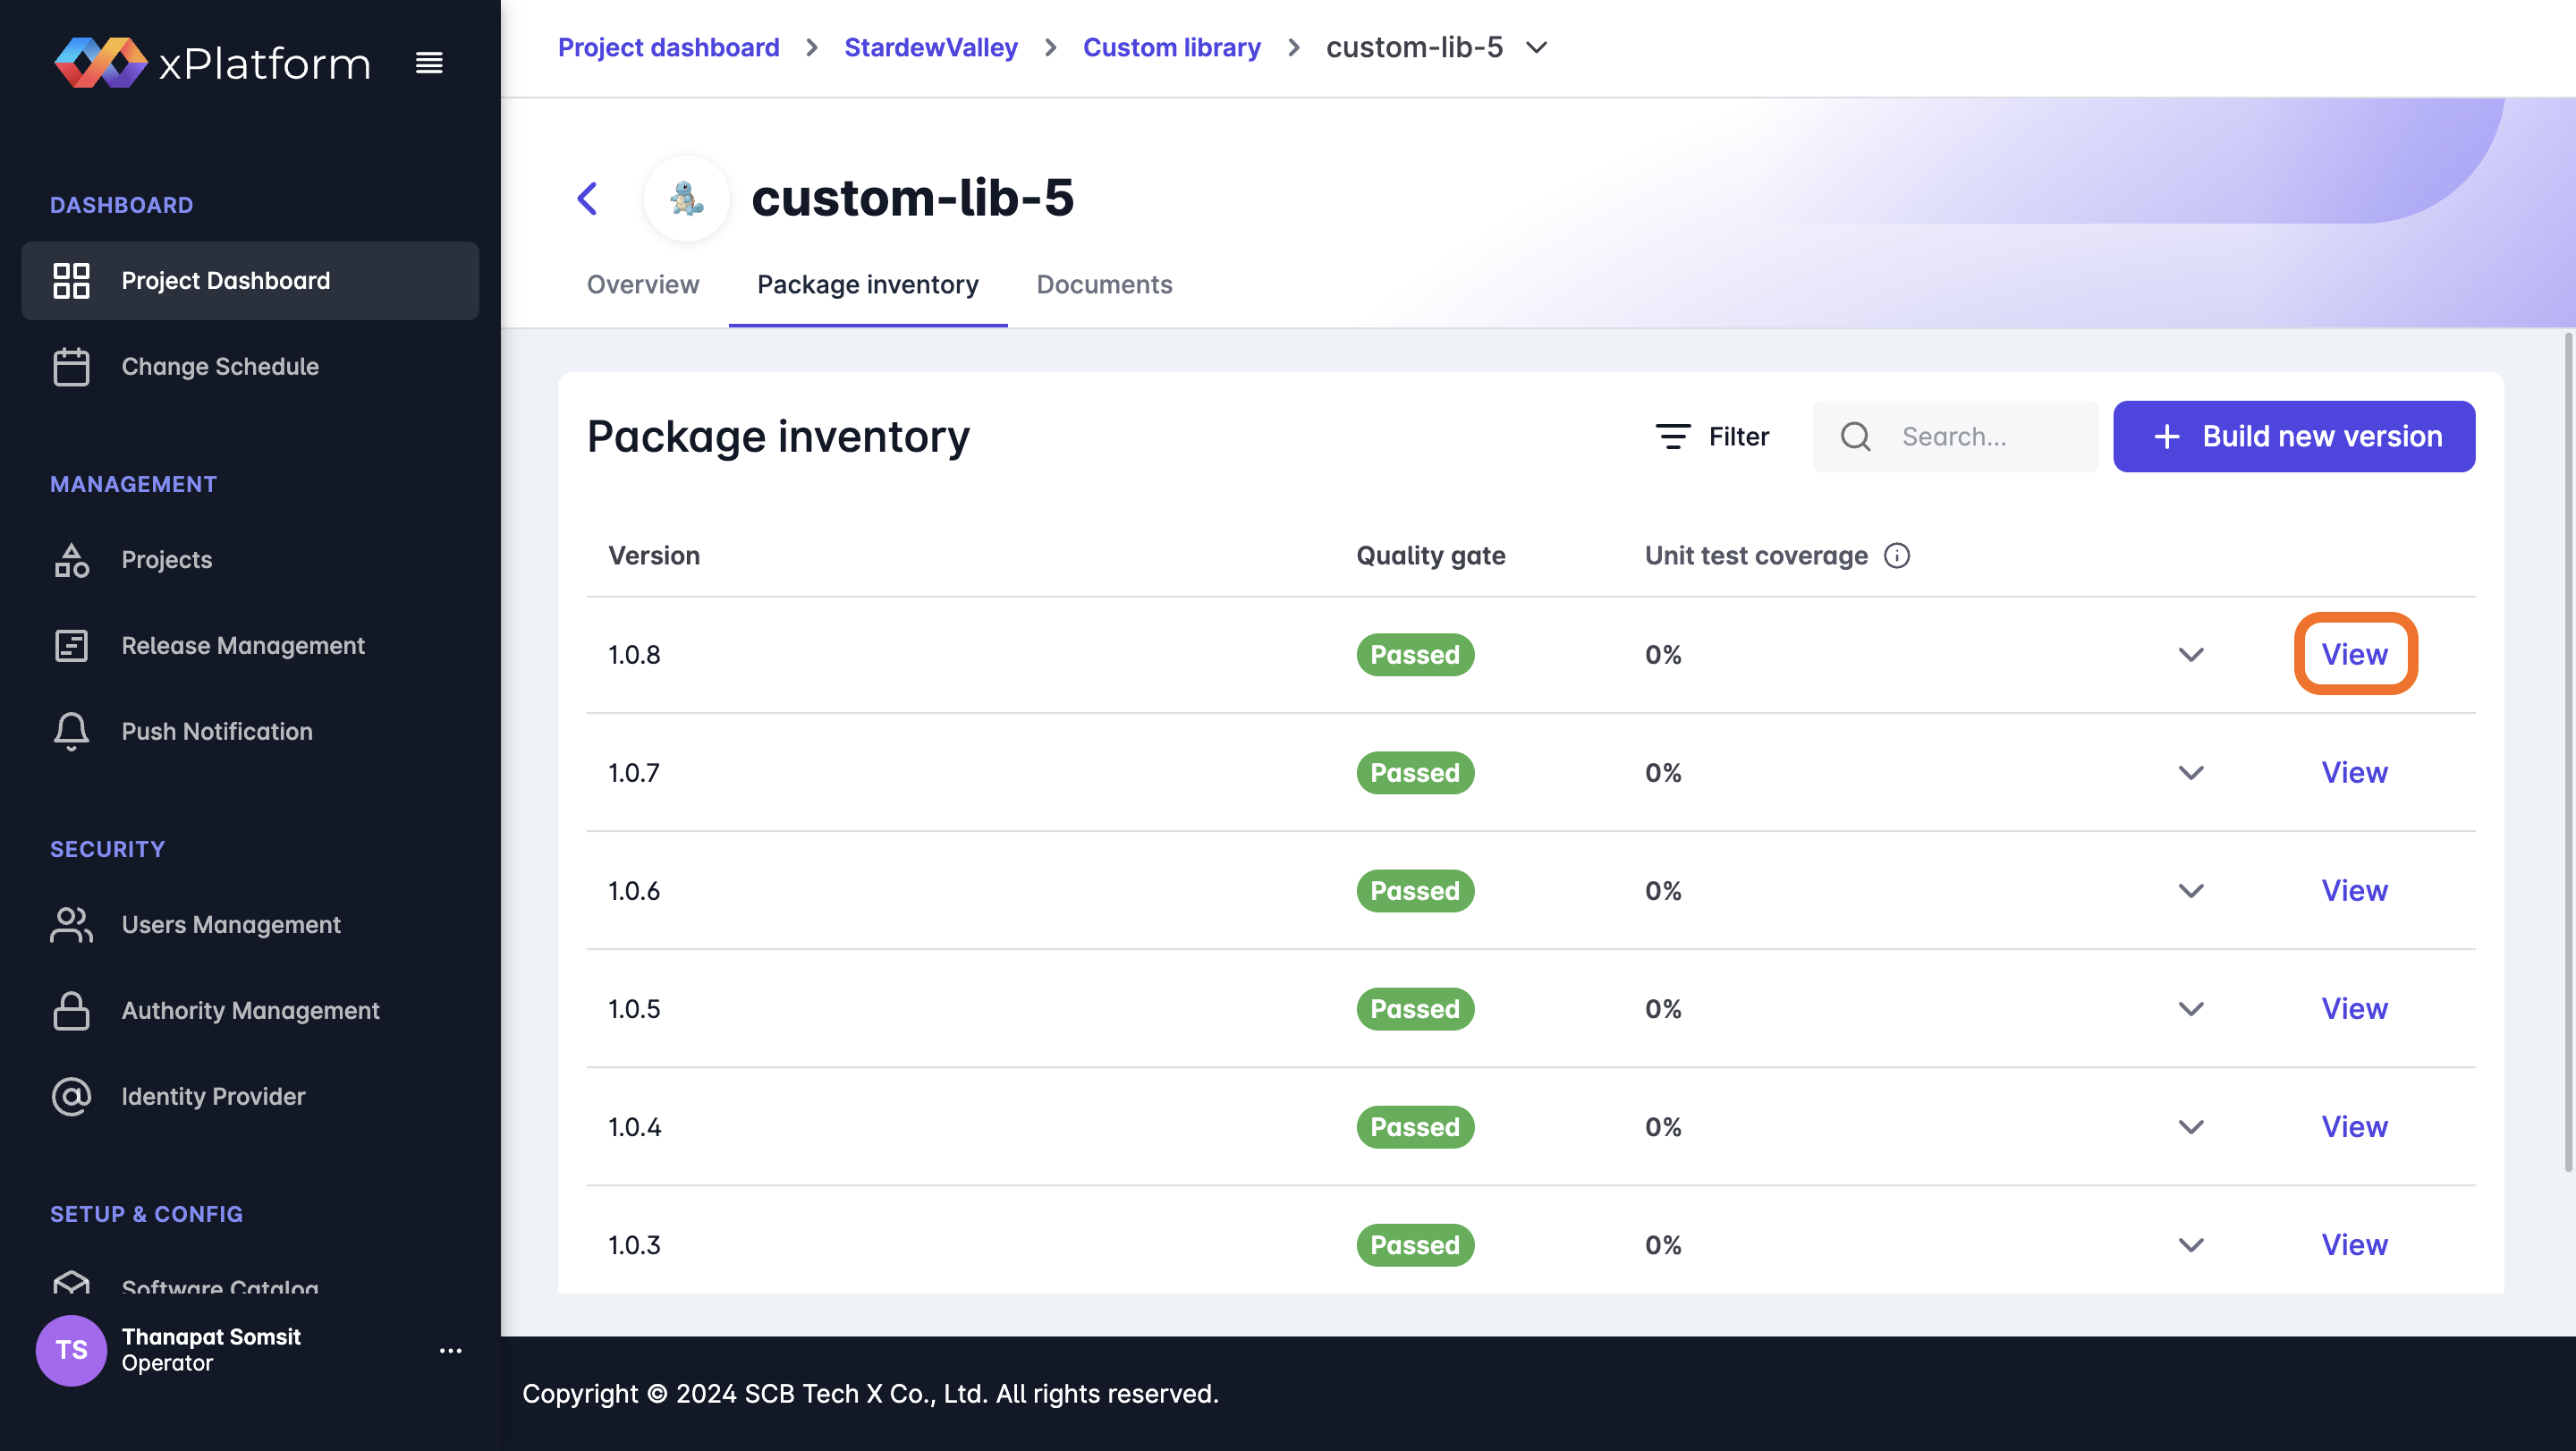
\includegraphics[width=\linewidth]{resources/pages/custom-library/update-library/7.png}
\end{center}

\begin{figure}[H]
    \begin{center}
        \includegraphics[width=\linewidth]{resources/pages/custom-library/update-library/8.png}
    
        \vspace{1in}
    
        \includegraphics[width=\linewidth]{resources/pages/custom-library/update-library/9.png}
    \end{center}
    \caption[การอัพเดตเวอร์ชัน Custom Library]{การอัพเดตเวอร์ชัน Custom Library}
  \label{fig:update-library}
\end{figure}


\newpage
\section{การใช้งานฟีเจอร์ Documentation}
\begin{center}
    \includegraphics[width=\linewidth]{resources/pages/documentation/1.png}

    \vspace{1in}

    \includegraphics[width=\linewidth]{resources/pages/documentation/2.png}
\end{center}

\begin{figure}[H]
    \begin{center}
        \includegraphics[width=\linewidth]{resources/pages/documentation/3.png}
    \end{center}
    \caption[การใช้งานฟีเจอร์ Documentation]{การใช้งานฟีเจอร์ Documentation}
  \label{fig:documentation}
\end{figure}

%% Display glossary (optional) -- need glossary option.
% \ifglossary\glossarypage\fi

%% Display index (optional) -- need idx option.
% \ifindex\indexpage\fi

% \begin{biosketch}
% \begin{center}
%   \includegraphics[width=1.5in]{mugshot.jpg}
% \end{center}
% Your biosketch goes here. Make sure it sits inside
% the \texttt{biosketch} environment.
% \end{biosketch}
\fi % \ifproject
\end{document}
